\documentclass[10pt,oneside]{article}
\usepackage[paperwidth=396.000bp,paperheight=594.000bp,top=42bp,bottom=34bp,left=52bp,right=52bp]{geometry}
\usepackage{fontspec}
\usepackage[russian,english]{babel}
\usepackage{amsmath}
\usepackage{microtype}
\usepackage{enumitem}
\usepackage{graphicx}
\usepackage{xcolor}
\usepackage[colorlinks=true,linkcolor=blue!55!black,urlcolor=blue!55!black]{hyperref}
\IfFontExistsTF{STIX Two Text}{\setmainfont{STIX Two Text}}{\IfFontExistsTF{PT Serif}{\setmainfont{PT Serif}}{\setmainfont{Times New Roman}}}
\setlength{\parindent}{1.15em}
\setlength{\parskip}{0pt}
\setlength{\emergencystretch}{2em}
\linespread{1.01}
\pagestyle{plain}
\newcommand{\TipsRunning}[1]{\par\vspace{2bp}{\centering\footnotesize #1\par}\vspace{2bp}}
\newcommand{\TipsSubsection}[1]{\par\vspace{6bp}{\normalsize\bfseries #1\par}\vspace{2bp}}
\newcommand{\TipsCaption}[1]{\par\vspace{4bp}{\footnotesize\bfseries #1\par}\vspace{2bp}}
\begin{document}
\begin{titlepage}
\centering
\vspace*{88bp}
{\fontsize{23}{27}\selectfont Советы Фейнмана по физике\par}
\vspace{16bp}
{\large Русская сборка, перевод gemini-3.5-flash-low\par}
\vfill
{\small Built from the local 2013 PDF text layer\par}
\end{titlepage}
\phantomsection
\pdfbookmark[1]{Contents}{tips-toc}
\tableofcontents
\clearpage
\phantomsection
\section*{Содержание}
\addcontentsline{toc}{section}{Содержание}
\pdfbookmark[1]{Содержание}{tips-sec-0-содержание}
\label{tips-sec-0-содержание}
\markboth{Содержание}{Содержание}
Содержание Предисловие ко второму изданию, vii Предисловие, ix Введение, xi Благодарности, xv Об истории создания «Фейнмановских лекций по физике», Воспоминания Мэтью Сэндса 1 Интервью с Ричардом Фейнманом 15 Интервью с Робертом Лейтоном 23 Интервью с Рохусом Фогтом 29 1 Вводные темы --- обзорная лекция A 35 2 Законы и интуиция --- обзорная лекция B 61 3 Задачи и их решения --- обзорная лекция C 91 4 Динамические эффекты и их применения 115 5 Избранные задачи 155 Источники иллюстраций, 179 Предметный указатель, 181\par

\clearpage
\phantomsection
\section*{Предисловие ко второму изданию}
\addcontentsline{toc}{section}{Предисловие ко второму изданию}
\pdfbookmark[1]{Предисловие ко второму изданию}{tips-sec-1-предисловие-ко-второму-изданию}
\label{tips-sec-1-предисловие-ко-второму-изданию}
\markboth{Предисловие ко второму изданию}{Предисловие ко второму изданию}
Предисловие ко второму изданию За шесть лет, прошедших с момента первой публикации книги Feynman’s Tips on Physics (Addison-Wesley, 2006), интерес к этому дополнению к The Feynman Lectures on Physics не ослабевал, о чем свидетельствует постоянно растущее число посетителей сайта The Feynman Lectures (www.feynmanlectures.info), созданного в связи с этим проектом: поступили тысячи запросов, во многих из которых сообщалось о предполагаемых опечатках в The Feynman Lectures, а во многих содержались вопросы и замечания по физическим задачам. Поэтому мы с большим удовольствием и гордостью представляем это второе издание Feynman’s Tips on Physics, выпущенное издательством Basic Books в рамках объединения печатных, аудио- и фотоправ, относящихся к The Feynman Lectures on Physics --- прав, которые на протяжении многих лет принадлежали различным издателям. В ознаменование этого счастливого события The Feynman Lectures on Physics (New Millennium Edition) теперь впервые печатается с макета LaTeX, что позволяет гораздо быстрее исправлять опечатки и в скором времени выпустить электронные издания «Лекций». Кроме того, это новое издание Feynman’s Tips on Physics выпускается в мягкой обложке по значительно сниженной цене по сравнению с оригиналом в твердом переплете и дополнено тремя содержательными интервью о «Лекциях»: • с Ричардом Фейнманом в 1966 году, вскоре после того, как завершилось его ключевое участие в проекте, • с Робертом Лейтоном в 1986 году, о лекторском даре Фейнмана --- и о трудностях перевода с «фейнмановского» языка на английский, и • с Рохусом Фогтом в 2009 году, о сообществе профессоров, совместно преподававших курс The Feynman Lectures в Калтехе. Всем, кто присылал по электронной почте или публиковал вопросы и замечания по поводу The Feynman Lectures on Physics и Feynman’s Tips on Physics, мы хотим выразить нашу искреннюю благодарность; ваш вклад и поддержка во многом помогли улучшить эти книги и будут оценены будущими поколениями читателей. Перед теми, кто писал с просьбой добавить больше задач, мы извиняемся за то, что они не смогли войти в это издание. Тем не менее, ваша поддержка вдохновила на создание новой обширной (готовой к публикации в ближайшее время) книги Exercises for The Feynman Lectures on Physics. Майкл А. Готтлиб Ральф Лейтон Ноябрь 2012\par

\clearpage
\phantomsection
\section*{Предисловие}
\addcontentsline{toc}{section}{Предисловие}
\pdfbookmark[1]{Предисловие}{tips-sec-2-предисловие}
\label{tips-sec-2-предисловие}
\markboth{Предисловие}{Предисловие}
Предисловие На одиноком пограничном посту высоко в Гималаях Рамасвами Баласубраманьян разглядывал в бинокль солдат Народно-освободительной армии Китая, дислоцированных в Тибете, --- которые, в свою очередь, рассматривали его в свои прицелы. Напряженность в отношениях между Индией и Китаем оставалась высокой в течение нескольких лет после 1962 года, когда между двумя странами произошла перестрелка на спорном участке границы. Солдаты НОАК, зная, что за ними наблюдают, дразнили Баласубраманьяна и его товарищей, индийских солдат, вызывающе размахивая высоко в воздухе своими карманными ярко-красными экземплярами «Цитат председателя Мао», более известных на Западе как «Маленькая красная книга Мао». Баласубраманьяну, бывшему тогда призывником и в свободное время изучавшему физику, эти насмешки вскоре надоели. Поэтому в один прекрасный день он пришел на свой наблюдательный пункт, подготовив достойный ответ. Как только солдаты НОАК снова начали размахивать в воздухе «Маленькой красной книгой Мао», он и двое других индийских солдат подняли и высоко держали три больших ярко-красных тома «Фейнмановских лекций по физике».\par

Однажды я получил письмо от господина Баласубраманьяна. Оно было одним из сотен писем, полученных мною за эти годы, в которых описывается глубокое влияние, которое Ричард Фейнман оказал на жизнь людей. Описав инцидент с «красными книгами» на китайско-индийской границе, он написал: «И вот, двадцать лет спустя, чьи красные книги все еще читают?»\par

И действительно. Сегодня, более чем через сорок лет после того, как они были прочитаны, «Фейнмановские лекции по физике» все еще читают --- и они по-прежнему вдохновляют людей, --- подозреваю, даже в Тибете.\par

Особый случай: несколько лет назад на одной вечеринке я встретил Майкла Готтлиба. Хозяин дома демонстрировал на экране компьютера гармонические обертоны живого тувинского горлового пения --- событие из тех, что делают жизнь в Сан-Франциско столь увлекательной. Готтлиб изучал математику и очень интересовался физикой, поэтому я посоветовал ему прочитать «Фейнмановские лекции по физике» --- и примерно через год он посвятил шесть месяцев своей жизни тому, чтобы очень внимательно прочитать эти «Лекции» от начала до конца. Как описывает Готтлиб в своем введении, это в конечном счете привело к появлению книги, которую вы сейчас читаете, а также к новому «Окончательному изданию» (Definitive Edition) «Фейнмановских лекций по физике».\par

x • ПРЕДИСЛОВИЕ\par

Поэтому мне приятно, что люди, интересующиеся физикой во всем мире, теперь могут изучать --- благодаря добавлению этого дополнительного тома --- более точное и полное издание «Фейнмановских лекций по физике», монументального труда, который будет продолжать обучать и вдохновлять студентов на протяжении грядущих десятилетий, будь то в центре Манхэттена или высоко в Гималаях.\par

Ральф Лейтон 11 мая 2005 г.\par

\clearpage
\phantomsection
\section*{Введение}
\addcontentsline{toc}{section}{Введение}
\pdfbookmark[1]{Введение}{tips-sec-3-введение}
\label{tips-sec-3-введение}
\markboth{Введение}{Введение}
1 Наша марка представлена во вкладыше к компакт-диску Back TUVA Future с участием мастера тувинского горлового пения Ондара и эпизодическим участием Ричарда Фейнмана (Warner Bros. 9 47131-2), выпущенному в 1999 году. 2 Feynman Lectures on Computation, автор Ричард Ф. Фейнман, под редакцией Энтони Дж. Г. Хея и Робина У. Аллена, 1996, Addison-Wesley, ISBN 0-201-48991-0.\par

Введение\par

Впервые я услышал о Ричарде Фейнмане и Ральфе Лейтоне в 1986 году благодаря их занимательной книге Surely You’re Joking, Mr. Feynman! Тринадцать лет спустя я встретил Ральфа на вечеринке. Мы подружились и в течение следующего года вместе работали над дизайном сувенирной марки в честь Фейнмана.1 Всё это время Ральф давал мне читать книги Фейнмана или книги о нём, включая (поскольку я программист) Feynman Lectures on Computation.2 Обсуждение квантовомеханических вычислений в этой увлекательной книге заинтриговало меня, но, не изучая ранее квантовую механику, я с трудом следил за ходом рассуждений. Ральф порекомендовал мне прочитать The Feynman Lectures on Physics Volume III: Quantum Mechanics, к чему я и приступил. Однако главы 1 и 2 третьего тома представляют собой перепечатку глав 37 и 38 первого тома, поэтому я обнаружил, что постоянно возвращаюсь к ссылкам в первом томе, вместо того чтобы продвигаться по третьему. В итоге я решил прочитать все «Фейнмановские лекции» от начала до конца --- я был полон решимости выучить квантовую механику! Однако со временем эта цель отошла на второй план, и я всё больше\par

Ричард Фейнман, около 1962 г.\par

x i i • В В Е Д Е Н И Е\par

погружался в удивительный мир Фейнмана. Радость познания физики --- просто ради самого удовольствия --- стала моим главным приоритетом. Я совершенно увлёкся! Примерно на середине первого тома я сделал перерыв в программировании и провёл шесть месяцев в сельской местности Коста-Рики, полностью посвятив себя изучению «Лекций».\par

Каждый день после полудня я разбирал новую лекцию и решал физические задачи, а по утрам повторял и вычитывал вчерашнюю лекцию. Я переписывался с Ральфом по электронной почте, и он воодушевил меня фиксировать все ошибки, которые попадались мне в первом томе. Это было не слишком обременительно, так как в этом томе ошибок оказалось совсем немного. Однако по мере продвижения по второму и третьему томам я с огорчением обнаруживал всё больше и больше опечаток. В конечном итоге я собрал в общей сложности более 170 ошибок в «Лекциях». Мы с Ральфом были удивлены: как можно было так долго не замечать столько ошибок? Мы решили выяснить, что можно сделать, чтобы исправить их в следующем издании.\par

Затем я обратил внимание на несколько интригующих фраз в предисловии Фейнмана:\par

«Причина, по которой здесь нет лекций о том, как решать задачи, заключается в том, что для этого существовали семинары. Хотя на первом курсе я действительно прочитал три лекции о методах решения задач, они сюда не вошли. Кроме того, была лекция об инерциальной навигации, которая, безусловно, должна следовать за лекцией о вращающихся системах, но, к сожалению, была опущена».\par

Это навело на мысль восстановить утерянные лекции и, если они окажутся интересными, предложить их Калтеху и Addison-Wesley для включения в более полное и исправленное издание «Лекций». Но сначала мне нужно было найти эти недостающие лекции, а я всё ещё находился в Коста-Рике! С помощью дедуктивной логики и небольшого расследования Ральфу удалось обнаружить конспекты лекций, которые ранее были спрятаны где-то между кабинетом его отца и архивами Калтеха. Ральф также раздобыл магнитофонные записи утерянных лекций, а занимаясь исследованием опечаток в архивах после своего возвращения в Калифорнию, я случайно обнаружил фотографии классной доски (которые долгое время считались утерянными) в коробке с различными негативами. Наследники Фейнмана великодушно дали нам разрешение на использование этих материалов, и, получив полезные критические замечания от Мэтта Сандса, единственного ныне живущего участника трио Фейнман–Лейтон–Сандс, мы с Ральфом реконструировали Обзор Б в качестве образца и представили его вместе со списком опечаток в Калтех и Addison-Wesley.\par

Издательство Addison-Wesley с энтузиазмом приняло наши идеи, но Калтех поначалу отнёсся к ним скептически. Тогда Ральф обратился к Кипу Торну, профессору теоретической физики имени Ричарда Фейнмана в Калтехе, которому в конце концов удалось достичь взаимопонимания между всеми участниками и который великодушно вызвался курировать нашу работу. Поскольку Калтех\par

\TipsRunning{В В Е Д Е Н И Е • x i i i}

3 Учебный год в Калтехе делится на три триместра: первый длится с конца сентября по начало декабря, второй --- с начала января по начало марта, а третий --- с конца марта по начало июня.\par

не хотел вносить изменения в существующие тома «Лекций» по историческим соображениям, Ральф предложил выпустить недостающие лекции отдельной книгой. Так появился этот дополнительный том. Он публикуется параллельно с новым Definitive Edition «Фейнмановских лекций по физике», в котором исправлены найденные мною ошибки, а также неточности, обнаруженные другими читателями.\par

Воспоминания Мэтта Сандса\par

В стремлении восстановить эти четыре лекции у нас с Ральфом возникало множество вопросов. Нам очень повезло получить ответы от профессора Мэтта Сандса --- человека, чьей идеей и было приступить к масштабному проекту по созданию «Фейнмановских лекций по физике». Мы удивились тому, что история их создания не была широко известна, и, понимая, что этот проект даёт возможность восполнить этот пробел, профессор Сандс любезно согласился написать воспоминания об истории возникновения «Фейнмановских лекций» для включения в это дополнение.\par

Четыре лекции\par

От Мэтта Сандса мы узнали, что в декабре 1961 года, под конец первого триместра3 курса физики для первокурсников, который Фейнман читал в Калтехе, было решено, что было бы несправедливо давать студентам новый материал всего за несколько дней до выпускного экзамена. Поэтому за неделю до контрольной работы Фейнман прочитал три необязательные обзорные лекции, в которых не вводилось нового материала. Эти обзорные лекции предназначались для студентов, испытывающих трудности в учёбе, и в них особое внимание уделялось методам понимания и решения физических задач. Некоторые из примеров задач имели историческое значение, включая открытие атомного ядра Резерфордом и определение массы пи-мезона. С присущей ему проницательностью Фейнман также разобрал решение задачи совсем другого рода, не менее важной по крайней мере для половины студентов его первого курса: эмоциональной проблемы осознания того, что ты оказался ниже среднего уровня.\par

Четвёртая лекция, «Динамические эффекты и их применение», была прочитана в начале второго триместра на первом курсе, вскоре после возвращения студентов с зимних каникул. Первоначально она должна была стать лекцией 21, и замысел её состоял в том, чтобы дать студентам отдохнуть от сложного теоретического обсуждения\par

x i v • В В Е Д Е Н И Е вращений, представленных в главах с 18 по 20, и показать студентам некоторые интересные приложения и явления, возникающие при вращении, «просто ради развлечения». Большая часть лекции была посвящена обсуждению технологии, которая была относительно новой в 1962 году: практической инерциальной навигации. В оставшейся части лекции обсуждались природные явления, возникающие при вращении, а также содержалась подсказка о том, почему Фейнман назвал исключение этой лекции из «Фейнмановских лекций по физике» «досадным».\par

После лекции Закончив лекцию, Фейнман часто оставлял микрофон включенным. Это предоставило нам уникальную возможность стать свидетелями того, как Фейнман общался со своими студентами. Приведенный здесь пример, записанный после лекции «Динамические эффекты и их применения», особенно примечателен обсуждением зарождающегося в 1962 году перехода в вычислениях реального времени от аналоговых методов к цифровым.\par

Упражнения В ходе этого проекта Ральф восстановил контакт с близким другом и коллегой своего отца Рохусом Фогтом, который любезно дал разрешение на переиздание упражнений и решений из сборника Exercises in Introductory Physics, созданного им и Робертом Лейтоном специально для «Лекций» еще в 1960-х годах. Из-за ограниченного объема книги я выбрал упражнения только к главам с 1 по 20 тома I (материал, пройденный до «Динамических эффектов и их применений»), предпочтя задачи, которые, говоря словами Роберта Лейтона, «численно или аналитически просты, но при этом глубоки и показательны по своему содержанию».\par

Сайт Читателям предлагается посетить сайт www.feynmanlectures.info для получения дополнительной информации об этом томе и «Фейнмановских лекциях по физике».\par

Майк Готтлиб Плайя-Тамариндо, Коста-Рика mg@feynmanlectures.info Майкл А. Готтлиб\par

\clearpage
\phantomsection
\section*{Благодарности}
\addcontentsline{toc}{section}{Благодарности}
\pdfbookmark[1]{Благодарности}{tips-sec-4-благодарности}
\label{tips-sec-4-благодарности}
\markboth{Благодарности}{Благодарности}
Благодарности Мы хотим выразить нашу искреннюю благодарность всем, кто сделал возможным появление этой книги, особенно: Томасу Томбрелло, руководителю отделения физики, математики и астрономии, за одобрение этого проекта от имени Калтеха; Карлу Фейнману и Мишель Фейнман, наследникам Ричарда Фейнмана, за разрешение опубликовать в этой книге лекции их отца; Мардж Л. Лейтон, за разрешение опубликовать отрывок из «Устной истории» (Oral History) Роберта Б. Лейтона, а также задачи из «Exercises in Introductory Physics»; Мэттью Сандзу, за его мудрость, знания, конструктивные замечания и предложения по рукописи --- а также за его проливающие свет мемуары; Рохусу Э. Фогту, за остроумные задачи и ответы в «Exercises in Introductory Physics», за интервью, которое он нам дал, и за разрешение использовать их в этом томе; Майклу Хартлу, за его тщательную вычитку рукописи и за его кропотливую работу над списком опечаток в «The Feynman Lectures on Physics»; Джону Ниру, за прилежное документирование лекций Фейнмана в Hughes Aircraft Corporation и за то, что он поделился этими записями с нами; Хелен Так, секретарю Фейнмана на протяжении многих лет, за ее поддержку и ободрение; Адаму Кокрану, за его непревзойденное умение ориентироваться в болоте запутанных книжных контрактов и личных отношений, чтобы найти новый дом для этой книги, а также для «The Feynman Lectures on Physics»; и Кипу Торну, за его благородство и неустанную работу по завоеванию доверия и поддержки всех участников, а также за руководство нашей работой.\par

\clearpage
\phantomsection
\section*{О происхождении «Фейнмановских лекций по физике»: мемуары Мэтью Сэндса}
\addcontentsline{toc}{section}{О происхождении «Фейнмановских лекций по физике»: мемуары Мэтью Сэндса}
\pdfbookmark[1]{О происхождении «Фейнмановских лекций по физике»: мемуары Мэтью Сэндса}{tips-sec-5-о-происхождении-фейнмановских-лекций-по-физике-мемуары-мэтью-сэндса}
\label{tips-sec-5-о-происхождении-фейнмановских-лекций-по-физике-мемуары-мэтью-сэндса}
\markboth{О происхождении «Фейнмановских лекций по физике»: мемуары Мэтью Сэндса}{О происхождении «Фейнмановских лекций по физике»: мемуары Мэтью Сэндса}
К истории создания «Фейнмановских лекций по физике» ВОСПОМИНАНИЯ МЭТТЬЮ СЭНДСА\par

Реформа образования в 1950-х годах Когда в 1953 году я впервые стал штатным преподавателем Калтеха, меня попросили вести несколько курсов для аспирантов. Я был весьма разочарован учебной программой аспирантуры. В течение первого года им читали курсы только по классической физике --- механике и электричеству с магнетизмом. (И даже курс электричества и магнетизма охватывал лишь статику, в нём вообще не было теории излучения.) Мне казалось позорным, что эти талантливые студенты не знакомились с идеями современной физики (многие из которых существовали уже от 20 до 50 или более лет) вплоть до второго или третьего года обучения в аспирантуре. Поэтому я начал кампанию за реформу этой программы. Я знал Ричарда Фейнмана ещё со времён нашей работы в Лос-Аламосе, и мы оба перешли в Калтех несколько лет назад. Я попросил Фейнмана присоединиться к этой кампании, мы набросали контуры новой программы и в конце концов убедили физический факультет принять её. Программа первого года состояла из курса электродинамики и электронной теории (его читал я), вводного курса квантовой механики (его читал Фейнман) и, насколько я помню, курса математических методов, который читал Роберт Уокер. Думаю, что новая программа оказалась весьма успешной.\par

Примерно в то же время Джеррольд Захариас из МТИ под впечатлением от появления Спутника начал продвигать программу по обновлению преподавания физики в средних школах США. Одним из результатов стало создание программы PSSC (Physical Science Study Committee), разработка множества новых материалов и идей, а также некоторые дискуссии.\par

Когда программа PSSC близилась к завершению, Захариас и его коллеги (среди которых, как мне кажется, были Фрэнсис Фридман и Филип Моррисон) решили, что пришло время взяться также и за пересмотр университетского курса физики. Они организовали пару крупных встреч преподавателей физики, итогом которых стало создание Комиссии по физике в колледжах (Commission on College Physics) --- национального комитета, состоящего из дюжины университетских преподавателей физики, который\par

2 • ВОСПОМИНАНИЯ МЭТТЬЮ СЭНДСА 1Упражнения в главе 5 настоящего тома включают более десятка задач из собрания Фостера Стронга, которые были с разрешения воспроизведены в Exercises in Introductory Physics Роберта Б. Лейтона и Рокуса Э. Вогта. поддерживался Национальным научным фондом и перед которым стояла задача стимулировать общенациональные инициативы по модернизации преподавания физики в колледжах и университетах. Захариас пригласил меня на те первые встречи, а позже я работал в этой Комиссии, со временем став её председателем.\par

Программа Калтеха Эта деятельность побудила меня задуматься о том, что можно сделать с программой обучения студентов младших курсов в Калтехе, которой я уже давно был довольно недоволен. Вводный курс физики основывался на книге Милликена, Роллера и Уотсона --- прекрасном учебнике, написанном, если не ошибаюсь, в 1930-х годах, который, несмотря на последующую переработку Роллером, содержал очень мало современной физики или не содержал её вовсе. Кроме того, курс преподавался без лекций, поэтому возможностей для введения нового материала было немного. Сильной стороной курса был сборник сложных «задач», составленный Фостером Стронгом1, которые использовались для еженедельных домашних заданий, и два еженедельных семинара, на которых студенты обсуждали эти задачи.\par

Как и другие преподаватели физики, каждый год я назначался куратором для нескольких студентов, специализирующихся по физике. Общаясь со студентами, я часто с огорчением замечал, что к третьему курсу они теряли интерес к продолжению занятий физикой --- по всей видимости, отчасти из-за того, что они изучали физику уже два года, но так и не познакомились ни с какими идеями современной науки. Поэтому я решил не ждать, пока созреет национальная программа, а попытаться сделать что-то в самом Калтехе. В частности, мне хотелось, чтобы некоторые разделы «современной» физики --- атомы, ядра, кванты и теория относительности --- вошли в вводный курс. После обсуждения с несколькими коллегами --- прежде всего с Томасом Лауритсеном и Фейнманом --- я предложил Роберту Бейчеру, тогдашнему заведующему кафедрой физики, начать программу реформирования вводного курса. Его первая реакция была не слишком обнадеживающей. По сути, он сказал: «Я повсюду говорю, что у нас прекрасная программа, которой я горжусь. Наши семинарские занятия ведут наши ведущие профессора. Зачем нам что-то менять?» Я настаивал, меня поддержали еще несколько коллег, так что Бейчер уступил, принял эту идею и вскоре получил грант от Фонда Форда (если я правильно помню, чуть больше миллиона долларов). Грант предназначался для покрытия расходов на разработку нового оборудования для вводного\par

ВОСПОМИНАНИЯ МЭТТЬЮ СЭНДСА • 3 2Principles of Modern Physics, Роберт Б. Лейтон, 1959, McGraw-Hill, номер карточки Каталога Библиотеки Конгресса 58-8847. лабораторий и для разработки нового содержания курса --- в частности, для привлечения временных преподавателей к выполнению обычных обязанностей тех, кто посвящал свое время проекту.\par

Когда грант был получен, Бэчер назначил небольшую рабочую группу для руководства программой: Роберта Лейтона в качестве председателя, Виктора Неера и меня. Лейтон уже давно участвовал в программе для старших курсов --- основой которой была его книга Principles of Modern Physics2, --- а Неер был известен как блестящий приборист. В то время я был раздосадован тем, что Бэчер не предложил мне возглавить эту группу. Я предполагал, что отчасти это могло быть связано с тем, что я и так был довольно сильно занят руководством Синхротронной лабораторией, но мне всегда казалось, что он также опасался моей излишней «радикальности» и хотел уравновесить проект консерватизмом Лейтона.\par

Комитет с самого начала согласился, что Неер сосредоточится на разработке новых лабораторных работ, по поводу которых у него было множество идей, а мы должны работать над подготовкой лекционного курса в следующем году, полагая, что лекции станут наилучшим инструментом для разработки нового содержания курса. Мы с Лейтоном должны были составить программу лекций. Мы начали с того, что независимо друг от друга составляли планы курса, но встречались каждую неделю, чтобы сравнить наши результаты и попытаться прийти к общему знаменателю.\par

Тупик и озарение\par

Вскоре стало ясно, что найти общий язык будет непросто. Мне подход Лейтона казался в основном перепевом содержания курсов физики, бывших в моде последние 60 лет. Лейтон же считал, что я продвигаю непрактичные идеи --- что первокурсники еще не готовы к «современному» содержанию, которое я хотел ввести. К счастью, моя решимость подкреплялась частыми беседами с Фейнманом. Фейнман уже тогда был широко известен как потрясающий лектор и умел особенно доходчиво объяснять идеи современной физики широкой аудитории. Возвращаясь домой из института, я часто заезжал к нему домой, чтобы поделиться своими мыслями и узнать его мнение; он часто подсказывал, что можно сделать, и в целом поддерживал меня.\par

После нескольких месяцев этих усилий я начал падать духом: я не понимал, как мы с Лейтоном вообще сможем договориться о программе. Наши концепции курса казались совершенно несовместимыми. И вот\par

4 • ВОСПОМИНАНИЯ МЭТТЬЮ СЭНДСА в один прекрасный день меня осенило: почему бы не попросить Фейнмана прочитать лекции по этому курсу? Мы могли бы дать ему наброски как Лейтона, так и мои, и предоставить ему самому решать, что делать. Я сразу же предложил эту идею Фейнману в таком духе: «Слушай, Дик, ты потратил сорок лет своей жизни на то, чтобы понять физический мир. Вот тебе возможность собрать всё это воедино и представить новому поколению учёных. Почему бы тебе не прочитать курс лекций первокурсникам в следующем году?» Он не сразу проявил энтузиазм, но в течение следующих нескольких недель мы продолжали обсуждать эту идею, и вскоре он увлекся замыслом. Он стал говорить, что, может быть, мы могли бы сделать то или это. Или что вот это подошло бы сюда, и всё в таком роде. После нескольких недель таких обсуждений он спросил меня: «А бывало ли когда-нибудь, чтобы великий физик читал курс лекций первокурсникам?» Я ответил, что, насколько мне известно, такого никогда не было. На это он сказал: «Я сделаю это».\par

Фейнман будет читать лекции\par

На следующем заседании нашего комитета я с большим энтузиазмом изложил своё предложение --- и был крайне разочарован прохладной реакцией Лейтона. «Это плохая идея. Фейнман никогда не преподавал студентам младших курсов. Он не знает, как разговаривать с первокурсниками и что они способны усвоить». Но положение спас Неер. Его глаза загорелись от восторга, и он сказал: «Это было бы здорово. Дик знает столько физики и умеет сделать её интересной. Было бы просто фантастически, если бы он действительно взялся за это». Лейтона удалось убедить, и, согласившись, он поддержал эту идею от всей души.\par

Несколько дней спустя я столкнулся со следующим препятствием. Я изложил эту идею Бэчеру. Он отнёсся к ней без особого восторга. Он считал, что Фейнман слишком важен для аспирантуры и его нельзя отвлекать. Кто будет читать квантовую электродинамику? Кто будет работать с аспирантами-теоретиками? И вообще, сможет ли он опуститься до уровня первокурсников? На этом этапе я провел некоторую работу с ведущими сотрудниками физического факультета, которые замолвили перед Бэчером словечко в поддержку этой идеи. И наконец, я использовал аргумент, столь близкий сердцу университетских кругов: если Фейнман действительно хочет это сделать, неужели вы хотите запретить ему? Решение было принято.\par

За шесть месяцев до первой лекции мы с Лейтоном рассказали Фейнману о наших соображениях. Он начал интенсивно работать над развитием собственных идей. По крайней мере раз в неделю я заходил к нему домой, и мы обсуждали то, о чём он размышлял. Иногда он спрашивал, считаю ли я тот или иной подход доступным для студентов, или думаю ли я, что то или это\par

...последовательность материала будет «работать» лучше всего. Я могу упомянуть конкретный пример. Фейнман работал над тем, как представить идеи интерференции и дифракции волн, и испытывал трудности с поиском подходящего математического подхода --- одновременно простого и мощного. Ему не удавалось найти такой подход без использования комплексных чисел. Он спросил меня, думаю ли я, что первокурсники справятся с алгеброй комплексных чисел. Я напомнил ему, что студентов, принятых в Калтех, отбирали в первую очередь по их продемонстрированным способностям в математике, и что я уверен в том, что у них не возникнет проблем с комплексной алгеброй, если дать им краткое введение в эту тему. Его двадцать вторая лекция содержит прекрасное введение в алгебру комплексных величин, которое он затем смог использовать во многих последующих лекциях для описания колеблющихся систем, для задач физической оптики и так далее.\par

В самом начале возникла небольшая проблема. У Фейнмана было давнее обязательство отсутствовать в Калтехе в течение третьей недели осеннего семестра, так что он должен был пропустить две лекции. Мы согласились, что эта проблема легко решается. В эти дни его заменю я. Однако, чтобы не нарушать непрерывность его изложения, я прочитал бы эти две лекции по некоторым вспомогательным темам, которые могли бы быть полезны студентам, но не были связаны с его основной линией развития. Это объясняет, почему главы 5 и 6 тома I стоят несколько особняком.\par

Однако по большей части Фейнман работал один над составлением подробного плана того, что он будет делать в течение всего года, прорабатывая детали в достаточной степени, чтобы быть уверенным в отсутствии непредвиденных трудностей. Он напряженно работал до конца того учебного года и к сентябрю (уже 1961 года) был готов начать свой первый год лекций.\par

Новый курс физики\par

Первоначально предполагалось, что лекции, прочитанные Фейнманом, станут отправной точкой для развития пересмотренной программы двухгодичного вводного курса --- обязательного для всех поступающих студентов Калтеха. Думали, что в последующие годы другие преподаватели возьмут на себя ответственность за каждый из этих двух лет, создав со временем полноценный «курс» --- с учебником, домашними заданиями, лабораторными работами и так далее. Однако для первых лет чтения лекций необходимо было разработать иной формат. Никаких учебных материалов не существовало, и их приходилось создавать по ходу дела. Были запланированы две часовые лекции --- в 11 часов утра по вторникам и четвергам, а также каждую неделю студенты распределялись на часовые семинары, которые проводил преподаватель или аспирант. Также каждую неделю проводилась трехчасовая лабораторная работа под руководством Нехера.\par

Во время лекций Фейнман носил микрофон, висевший у него на шее и подключенный к магнитофону в другой комнате. Содержимое классных досок периодически фотографировалось. Обе эти службы обеспечивались Томом Харви, техническим ассистентом, заведующим лекционным залом. Харви также помогал Фейнману готовить редкие демонстрационные опыты для лекций. Записанные лекции перепечатывались в довольно разборчивом виде машинисткой Джули Курсио.\par

В тот первый год Лейтон взял на себя ответственность за то, чтобы стенограммы редактировались для ясности и как можно быстрее, дабы студенты получали напечатанные конспекты лекций для изучения вскоре после их прочтения. Сначала думали, что эту работу можно выполнить, поручив каждую лекцию одному из аспирантов, которые вели семинары и лабораторные работы. Однако это себя не оправдало, так как у аспирантов уходило на это слишком много времени, а полученный результат отражал скорее идеи аспиранта, нежели Фейнмана. Лейтон быстро изменил порядок, взяв большую часть работы на себя и привлекая различных преподавателей (с физического и инженерного факультетов) для редактирования одной или нескольких лекций. В соответствии с этим планом в течение первого года я также отредактировал несколько лекций.\par

На второй год курса были внесены некоторые изменения. Лейтон взял на себя ответственность за студентов первого курса --- он читал лекции и в целом руководил курсом. К счастью, теперь у студентов с самого начала имелись расшифрованные конспекты лекций Фейнмана за прошлый год. Я стал отвечать за детали курса второго года, лекции на котором теперь читал Фейнман. На меня также легла обязанность своевременно готовить отредактированные стенограммы. Из-за характера материала второго года я пришел к выводу, что наиболее целесообразно взять эту задачу на себя.\par

Я также присутствовал почти на всех лекциях --- как и в первый год --- и взял себе одну из групп семинарских занятий, чтобы видеть, как студенты усваивают курс. После каждой лекции Фейнман, Джерри Нойгебауэр и я (иногда с одним или двумя другими коллегами) обычно отправлялись обедать в студенческую столовую, где обсуждали, какие домашние задания по теме лекции лучше дать студентам. У Фейнмана обычно уже было в голове несколько идей для этих задач, а другие рождались в ходе дискус...\par

ВОСПОМИНАНИЯ МЭТЬЮ СЭНДСА • 7 ...куссии. Нойгебауэр отвечал за сбор этих упражнений и еженедельную подготовку «заданий».\par

Какими были лекции\par

Присутствовать на лекциях было огромным удовольствием. Фейнман появлялся минут за пять до назначенного начала лекции. Он доставал из нагрудного кармана рубашки один-два маленьких клочка бумаги --- примерно 5 на 9 дюймов, --- разворачивал их и разглаживал в центре демонстрационного стола в передней части лекционной аудитории. Это были его заметки к лекции, хотя он редко в них заглядывал. (На фотографии, приведенной в начале главы 19 тома II, Фейнман запечатлен во время одной из своих лекций стоящим за демонстрационным столом, на котором видны два листка заметок.) Как только звенел звонок, возвещающий о начале официального занятия, он начинал лекцию. Каждая лекция представляла собой тщательно продуманную драматическую постановку, которую он, очевидно, детально планировал --- обычно с введением, развитием темы, кульминацией и развязкой. И его чувство времени было поразительным. Лишь в очень редких случаях он заканчивал лекцию более чем на долю минуты раньше или позже конца часа. Даже использование классных досок в передней части аудитории казасело тщательно отрепетированным. Он начинал в верхнем левом углу первой доски слева, а к концу лекции как раз полностью заполнял вторую доску с правого края.\par

Но самым большим удовольствием было, конечно же, наблюдать за развитием оригинальной последовательности идей, излагаемых с ясностью и изяществом.\par

Решение о создании книги\par

Хотя изначально мы не предполагали, что стенограммы лекций станут книгой, эта идея всерьез обсуждалась примерно в середине второго года чтения лекций --- весной 1963 года. Эта мысль была вызвана отчасти запросами физиков из других учебных заведений о возможности предоставления им стенограмм, а отчасти предложениями нескольких книжных редакторов --- до которых, разумеется, дошли слухи о читаемом курсе и которые, возможно, видели копии стенограмм, --- о том, что нам следует подумать о книге и что они хотели бы ее опубликовать.\par

После некоторого обсуждения мы решили, что при определенных усилиях стенограммы можно превратить в книгу, поэтому мы попросили заинтересованных издателей\par

8 • ВОСПОМИНАНИЯ МЭТЬЮ СЭНДСА представить нам свои предложения по этому поводу. Наиболее привлекательное предложение поступило от представителей издательства Addison-Wesley Publishing Company (A-W), которые предложили предоставить нам книги в твердом переплете к началу занятий в сентябре 1963 года --- всего через шесть месяцев после принятия решения о публикации. Кроме того, учитывая, что мы не требовали выплаты авторских гонораров, они предложили выпустить книги по довольно низкой цене.\par

Столь быстрый график публикации был возможен благодаря тому, что издательство располагало всеми необходимыми собственными возможностями и штатом сотрудников для редактирования, набора и офсетной печати. И благодаря использованию нового (по тем временам) формата, состоящего из одной широкой колонки текста и очень широкого поля с одной стороны, они могли разместить рисунки и другие вспомогательные материалы. Такой формат означал, что материалы, которые обычно были бы гранками, можно было использовать непосредственно для окончательной верстки страниц, без необходимости заново набирать текст для размещения рисунков и тому подобного.\par

Предложение A-W одержало верх. Я взял на себя задачу внесения необходимых исправлений и примечаний в стенограммы лекций и в целом работы с издательством --- чтения корректуры набранного материала и так далее. (Лейтон в это время был сильно занят преподаванием курса для первокурсников по второму кругу.) Я редактировал стенограмму каждой лекции с точки зрения ясности и точности, затем отдавал ее Фейнману на окончательную проверку и, как только накапливалось несколько готовых лекций, отправлял их в A-W.\par

Я довольно быстро отправил первые несколько лекций и вскоре получил обратно гранки для корректуры. Это была катастрофа! Редактор в A-W подверг текст значительной переработке, превратив разговорный стиль стенограмм в традиционный, академический стиль учебника --- заменяя «вы» на «некто» и тому подобное. Опасаясь возможного конфликта по этому поводу, я позвонил редактору. После того как я объяснил, что мы считаем неформальный, разговорный стиль неотъемлемой частью лекций и предпочитаем личные местоимения безличным, она все поняла и в дальнейшем проделала отличную работу, по большей части оставляя всё как есть. (После этого работать с ней было одно удовольствие, и мне жаль, что я не помню ее имени.)\par

Следующий камень преткновения оказался более серьезным: выбор названия для книги. Я помню, как однажды пришел к Фейнману в его кабинет, чтобы обсудить этот вопрос. Я предложил выбрать простое название вроде «Physics» или «Physics One», а авторами указать Фейнмана, Лейтона и Сэндса. Предложенное название ему не особенно понравилось, а реакция на предлагаемый состав авторов была довольно бурной: «С какой стати там должны быть ваши имена? Вы ведь выполняли лишь работу стенографиста!» Я не согласился, указав, что без усилий Лейтона и моих собственных лекции никогда бы не превратились в\par

ВОСПОМИНАНИЯ МЭТТЬЮ СЭНДЗА • 9 книге. Разногласия разрешились не сразу. Через несколько дней я вернулся к этому обсуждению, и вместе мы пришли к компромиссу: «“Фейнмановские лекции по физике” Фейнмана, Лейтона и Сэндза».\par

Предисловие Фейнмана\par

После завершения второго года лекций --- примерно в начале июня 1963 года --- я сидел у себя в кабинете и выставлял оценки за выпускные экзамены, когда зашел Фейнман, чтобы попрощаться перед отъездом из города (кажется, в Бразилию). Он спросил, как студенты справились с экзаменом. Я ответил, что, по-моему, довольно хорошо. Он спросил, какой средний балл, и я назвал его --- насколько помню, что-то около 65 процентов. Он отреагировал так: «О, это ужасно, они должны были справиться лучше. Я потерпел неудачу». Я попытался разубедить его в этом, указывая на то, что средний балл весьма условен и зависит от многих факторов, таких как сложность предложенных задач, используемая система оценки и тому подобное, и что мы обычно старались сделать средний балл достаточно низким, чтобы получить некоторый разброс оценок для построения разумного «распределения» при выставлении буквенных оценок. (К слову, сегодня я бы не одобрил такой подход.) Я сказал, что, на мой взгляд, многие студенты явно вынесли очень многое из этих занятий. Но его это не убедило.\par

Тогда я сказал ему, что подготовка «Лекций» к публикации идет полным ходом, и спросил, не хочет ли он написать какое-нибудь предисловие. Идея его заинтересовала, но у него не хватало времени. Я предложил включить диктофон, стоявший у меня на столе, чтобы он мог продиктовать свое предисловие. И вот, все еще переживая из-за низкого среднего балла на выпускном экзамене студентов второго курса, он надиктовал первый набросок «Предисловия Фейнмана», которое вы найдете в начале каждого тома «Лекций». В нем он говорит: «Мне кажется, я не очень хорошо справился со своей задачей перед студентами». Я часто сожалел о том, что устроил запись предисловия именно таким образом, поскольку не считаю это суждение достаточно обдуманным. И я боюсь, что многие преподаватели использовали его как оправдание для того, чтобы не пробовать заниматься по «Лекциям» со своими студентами.\par

Второй и третий тома\par

История публикации второго года лекций немного отличается от первого. Во-первых, когда второй год подошел к концу (это было примерно в июне 1963 года), было решено разделить конспекты лекций на две части, чтобы составить два отдельных тома: «Электричество и магнетизм» и «Квантовая\par

1 0 • ВОСПОМИНАНИЯ МЭТТЬЮ СЭНДЗА физика». Во-вторых, считалось, что конспекты лекций по квантовой физике можно значительно улучшить за счет некоторых дополнений и довольно существенной переработки. С этой целью Фейнман предложил в конце следующего года прочесть ряд дополнительных лекций по квантовой физике, которые можно было бы объединить с первоначальным курсом для составления третьего тома печатного издания лекций.\par

Возникло и дополнительное осложнение. Примерно за год до этого федеральное правительство одобрило строительство в Стэнфордском университете двухмильного линейного ускорителя для получения электронов с энергией 20 ГэВ для исследований в области физики элементарных частиц. Это должен был быть самый крупный и дорогой ускоритель из когда-либо построенных, с энергиями и интенсивностями электронов, во много раз превышающими показатели любой существующей установки --- захватывающий проект. Больше года В. К. Х. Панофский, назначенный директором недавно созданной лаборатории --- Стэнфордского центра линейного ускорителя --- пытался убедить меня присоединиться к нему в качестве заместителя директора, чтобы помочь в строительстве нового ускорителя. Весной того года он меня уговорил, и я согласился переехать в Стэнфорд в начале июля. Однако я был обязан довести «Лекции» до конца, поэтому часть соглашения состояла в том, что я заберу эту работу с собой. Оказавшись в Стэнфорде, я обнаружил, что мои новые обязанности требуют больше сил, чем я ожидал, так что мне приходилось работать над «Лекциями» почти каждый вечер, чтобы двигаться вперед в нужном темпе. Мне удалось завершить окончательное редактирование второго тома к марту 1964 года. К счастью, неоценимую помощь мне оказывала моя новая и очень способная секретарь Патриция Пройсс.\par

К маю того года Фейнман прочитал дополнительные лекции по квантовой физике, и мы начали работу над третьим томом. Поскольку требовалась серьезная перестройка структуры и переработка материала, я несколько раз ездил в Пасадину для длительных консультаций с Фейнманом. Все трудности были легко преодолены, и материалы для третьего тома были подготовлены к декабрю.\par

Реакция студентов\par

Общаясь со студентами на своих семинарских занятиях, я мог составить довольно четкое представление о том, как они реагировали на лекции. Полагаю, многие, если не большинство из них, понимали, что им выпала редкая возможность. Я также видел, что они часто увлекались захватывающими идеями и многому учились в физике. Разумеется, это относилось не ко всем студентам. Не стоит забывать, что этот курс был обязательным для всех первокурсников, хотя менее половины из них планировали специализироваться по физике, так что многие остальные, по сути, составляли подневольную аудиторию. Кроме того, выявились некоторые недостатки курса. В качестве при...\par

М Е М У А Р Ы  М Э Т Т Ь Ю  С Э Н Д С А • 1 1 мер, студентам часто было трудно отделить ключевые идеи лекций от некоторого второстепенного материала, введенного для иллюстрации практического применения.\par

Это особенно расстраивало их при подготовке к экзаменам.\par

В специальном предисловии к Юбилейному изданию «Фейнмановских лекций по физике» Дэвид Гудстейн и Джерри Нойгебауэр написали, что « .\par

.\par

.\par

по мере продолжения курса посещаемость со стороны зарегистрированных студентов начала угрожающе падать». Я не знаю, откуда они взяли эту информацию.\par

И мне интересно, какие у них есть доказательства того, что: «Многие студенты страшились занятий .\par

.\par

.\par

» Гудстейна в то время не было в Калтехе.\par

Нойгебауэр был частью команды, работавшей над курсом, и иногда в шутку говорил, что в лекционном зале не осталось студентов бакалавриата --- только аспиранты.\par

Возможно, это наложило отпечаток на его воспоминания.\par

Я сидел в конце зала на большинстве лекций, и мои воспоминания --- конечно, притупившиеся с годами --- говорят о том, что, возможно, процентов 20 или около того студентов не утруждали себя посещением.\par

Такое количество не было бы необычным для большой лекционной аудитории, и я не помню, чтобы кто-то был «встревожен». И хотя, возможно, были студенты в моей семинарской группе, которые страшились занятий, большинство были вовлечены и увлечены лекциями --- хотя некоторые из них, весьма вероятно, страшились домашних заданий.\par

Я хотел бы привести три иллюстрации того влияния, которое лек- ции оказали на студентов в те первые два года.\par

Первый случай относится ко времени, когда читался этот курс, и хотя это было более 40 лет назад, он произвел на меня такое впечатление, что я помню его отчетливо.\par

Это было в самом начале второго года, и по чистой случайности в расписании моя семинарская группа впервые собралась как раз перед первой лекцией Фейнмана в том году.\par

Поскольку лекции для обсуждения у нас еще не было, а домашнее задание еще не было задано, было неясно, о чем говорить.\par

Я начал занятие с того, что попросил студентов поделиться своими впечатлениями о лекциях предыдущего года, которые закончились примерно три месяца назад.\par

После нескольких ответов один студент сказал, что его заинтересовало обсуждение структуры глаза пчелы и того, как она была оптимизирована за счет баланса между эффектами геометрической оптики и Второй пример содержится в письме, полученном мной в 1997 году --- примерно через 34 года после чтения лекций --- от студента Билла Саттертуэйта, ограничениями, обусловленными волновой природой света (см. «Фейнмановские лекции по физике» (FLP), том\par

I, раздел 36-4).\par

Я спросил, сможет ли он восстановить эти рассуждения.\par

Он подошел к доске и почти без подсказок с моей стороны смог воспроизвести основные элементы этого доказательства.\par

И это спустя примерно шесть месяцев после лекции и без какого-либо повторения.\par

1 2 • В О С П О М И Н А Н И Я  М Э Т Т Ь Ю  С Э Н Д С А который посещал лекции, а также мою семинарскую группу.\par

Письмо пришло совершенно неожиданно, поводом для него стала его встреча с моим старым другом в MIT.\par

Он писал: «Этим письмом я хочу выразить благодарность вам и всем остальным за фейнмановскую физику.\par

.\par

.\par

.\par

Д-р\par

В предисловии Фейнмана говорится, что он не считает, что принес студентам много пользы.\par

.\par

.\par

.\par

Я не согласен.\par

Я и мои друзья всегда получали от них удовольствие и понимали, каким уникальным и прекрасным опытом они были.\par

И мы многому научились.\par

Что касается объек- тивных доказательств нашего отношения, я не помню, чтобы какая-либо другая регулярная лекция за время моей учебы в Калтехе сопровождалась аплодисментами, а моя память подсказывает, что в конце лекций д-ра\par

Фейнмана это происходило довольно часто.\par

.\par

.\par

.\par

» Последний пример относится к событиям нескольконедельной давности.\par

Мне довелось чи- тать автобиографический очерк, написанный Дугласом Ошеровым, который был удостоен Нобелевской премии по физике за 1996 год (совместно с Дэвидом Ли и Робертом Ричардсоном) за открытие сверхтекучести гелия-3.\par

Ошеров писал: «Это было хорошее время для учебы в Калтехе, так как Фейнман вел свой знаменитый курс лекций для сту- дентов младших курсов.\par

Этот двухгодичный цикл лекций стал чрезвычайно важной частью моего образования.\par

Хотя я не могу сказать, что всё понял, я думаю, что это внесло наибольший вклад в развитие моей физической интуиции». Послесловие Мой довольно резкий уход из Калтеха сразу после второго года лекций означал, что у меня не было возможности наблюдать за последу- ющим развитием вводного курса физики.\par

Поэтому я мало что знаю об эффективности опубликованных лекций для последующих студентов.\par

Всегда было ясно, что сами по себе «Лекции» не могут служить учебником.\par

В них отсутствует слишком много привычных атрибутов учебника: краткие обзоры глав, разобранные иллюстративные примеры, упражнения для домашней работы и так далее.\par

Их должны были предоставить усердные преподаватели, и некоторые из них были подготовлены Лейтоном и Рохусом Фогтом, которые взяли на себя ответственность за курс после 1963 года.\par

Одно время я предполагал, что они могут быть изданы в виде дополнительного тома, но это так и не осуществилось.\par

Во время своих поездок, связанных с Комиссией по физике в колледжах, я часто встречался с преподавателями физики в различных университетах.\par

Я слышал, что большинство преподавателей не считали «Лекции» подходящими для использования на своих занятиях --- хотя я также слышал от некоторых, что они использовали ту или иную книгу в классах повышенного уровня («honors») или в качестве дополнения к обычному учебнику.\par

(Должен сказать, что у меня часто складывалось впечатление, что некоторые преподаватели были\par

ВОСПОМИНАНИЯ МЭТТЬЮ СЭНДСА • 1 3 ...опасались браться за «Лекции» из-за страха, что студенты будут задавать вопросы, на которые они не смогут ответить.) Чаще всего мне приходилось слышать, что аспиранты находят «Лекции» прекрасным источником для повторения материала перед квалификационными экзаменами.\par

Похоже, за рубежом «Лекции» оказали даже большее влияние, чем в Соединенных Штатах. Издатель позаботился о переводе «Лекций» на множество языков --- насколько я помню, на двенадцать. И когда я ездил за границу на конференции по физике высоких энергий, меня часто спрашивали, не тот ли я самый Сэндс из «красных книг». К тому же я нередко слышал, что «Лекции» используются в вводных курсах физики.\par

Еще одним прискорбным последствием моего ухода из Калтеха стало то, что я больше не мог поддерживать тесное общение с Фейнманом и его женой Гвинет. Нас связывали теплые коллегиальные отношения еще со времен Лос-Аламоса, а в середине 1950-х годов я присутствовал на их свадьбе. В те редкие случаи после 1963 года, когда я бывал в Пасадене, я останавливался у них, а если приезжал с семьей, мы всегда проводили вечер вместе. Во время нашей последней встречи он рассказал нам о своей недавней операции по поводу рака, который вскоре после этого унес его жизнь.\par

Мне доставляет огромное удовольствие то, что сейчас, спустя примерно сорок лет после того, как они были прочитаны, «Фейнмановские лекции по физике» все еще печатаются, покупаются, читаются и, смею думать, ценятся по достоинству.\par

Санта-Круз, Калифорния 2 декабря 2004 г.\par

\clearpage
\phantomsection
\section*{Интервью с Ричардом Фейнманом}
\addcontentsline{toc}{section}{Интервью с Ричардом Фейнманом}
\pdfbookmark[1]{Интервью с Ричардом Фейнманом}{tips-sec-6-интервью-с-ричардом-фейнманом}
\label{tips-sec-6-интервью-с-ричардом-фейнманом}
\markboth{Интервью с Ричардом Фейнманом}{Интервью с Ричардом Фейнманом}
Интервью с Ричардом Фейнманом Из интервью с Ричардом Фейнманом, проведенного Чарльзом Вейнером в Альтадене, штат Калифорния, 4 марта 1966 года, любезно предоставлено Библиотекой и архивом Нильса Бора Американского инсти- тута физики, Колледж-Парк, штат Мэриленд, США. Фейнман: The Feynman Lectures on Physics. Хотите поговорить об этом? Вейнер: Думаю, это уместно, поскольку в тот период это была очень важная работа. Фейнман: Да. Интересно, сейчас, когда я думаю об этом: раз уж это было главным делом в тот период, а я жаловался, что не занимаюсь никакими исследованиями --- я действительно сумасшедший! Сейчас мне указывают на то, что с моей стороны глупо чувствовать себя так, будто я ничего не делал в те годы, ведь эта штука [The Feynman Lectures on Physics] --- это нечто значительное. Но я всё равно этого не чувствую, потому что в молодости ты посвящаешь себя какому-то идеалу --- тому, что собираешься совершать открытия в физике, --- и если занимаешься чем-то другим, тебе трудно объяснить себе, почему это должно приносить удовлетворение; ведь я просто вел занятия.\par

В общем, история этих лекций такова. Какая-то группа, в которую я не входил, обсуждала необходимость переделать курс физики, потому что многие способные студенты, изучавшие физику, жаловались, что после года или двух учебы все, чем они занимались, --- это бузиновые шарики и наклонные плоскости. В школе они так много слышали о теории относительности, странных частицах и чудесах мира, а здесь они не увидели бы ничего из этих чудес, пока не стали бы аспирантами. Это было очень тяжело, и они пытались перестроить курс физики. В итоге они разработали какую-то программу курса, и встал вопрос: кто будет его вести? Не знаю, как они договаривались между собой, но в конце концов ко мне пришел Сэндс и уговорил меня прочитать этот курс.\par

Впрочем, программу я выбросил. Понимаете, я, конечно, решил вести его по-своему. Но общую идею того, что требовалось сделать, я уловил.\par

1 6 • И Н Т Е Р В Ь Ю  С  Р И Ч А Р Д О М  Ф Е Й Н М А Н О М\par

Они хотели, чтобы я читал лекции первокурсникам. Они хотели перестроить курс. Раньше в нем не было общих лекций, которые читал бы ведущий преподаватель, а были отдельные группы, в которых преподавали аспиранты. Единственное, ради чего они тогда собирались вместе, --- это своего рода факультативная культурно-просветительская лекция, не связанная напрямую с курсом, раз в неделю по пятницам или, может быть, раз в две недели по пятницам.\par

Вейнер: Возможно, что-то историческое?\par

Фейнман: Ну, вещи бывали разные. Меня часто приглашали туда выступить, и я рассказывал о теории относительности. Это не входило в их курс. Иногда люди говорили о чем-то, что непосредственно относилось к их курсу, но все это не было скоординировано.\par

Теперь они собирались создать новую лабораторию. Они собирались состряпать новый практикум и придумывали новые эксперименты для него. Они собирались перестроить его так, чтобы ведущий профессор читал как минимум две лекции в неделю, плюс проводились бы семинарские занятия под руководством аспирантов. И вот, не прочитаю ли я эти лекции, понимаете? На эту перестройку у них были деньги от Фонда Форда. В те дни на изменение мира крутилось много денег.\par

И я сказал: «Ладно». Я принял этот вызов на один год и попытался составить курс, требующий чтения двух лекций в неделю.\par

Вейнер: Разве вам не пришлось бросить всю остальную работу, все остальное преподавание?\par

Фейнман: На самом деле пришлось. Мне самому верится с трудом, но жена говорит, что я работал практически день и ночь, по шестнадцать часов в сутки, постоянно. Я все время торчал здесь, беспокоясь об этих... работая над этими лекциями, потому что мне нужно было не только подготовить материал, но и выстроить саму лекцию так, чтобы она получилась хорошей, если вы понимаете, о чем я.\par

У меня была идея --- я сформулировал для себя своего рода принцип, ряд принципов. Первый состоял в том, что я не буду учить их ничему такому, что потом придется переучивать из-за того, что оно неверно, если только сразу не укажу на эту неверность. Например, если законы Ньютона являются лишь приближенными и не работают в квантовой механике и теории относительности, я начинаю с того, что говорю об этом, чтобы они понимали, где находятся. Другими словами, всегда должна быть какая-то карта. На самом деле я даже думал составить некую большую карту вещей с их взаимосвязями, чтобы мы видели, где находимся. Мне казалось, что одна из проблем всех курсов физики заключалась в том, что там просто говорили: вы учите вот это, учите вот то, а когда дойдете до конца, то поймете связ...\par

И Н Т Е Р В Ь Ю  С  Р И Ч А Р Д О М  Ф Е Й Н М А Н О М • 1 7 ...связей. Но ведь нет никакой карты, «путеводителя для растерянных», понимаете? Поэтому я хотел составить карту. Но оказалось, что это невыполнимая задача. В общем, я так и не составил этой карты.\par

Другое дело --- мне хотелось, чтобы в курсе было достаточно материала, над которым мог бы поломать голову способный студент, и в то же время чтобы его понимал и средний парень. Поэтому я попытался кое-что изобрести.\par

Позвольте мне перечислить эти принципы. Первый заключался в том, что я никогда не вводил ничего не совсем точного без объяснения того, что это не так и что именно изменится в следующий раз. (Кроме того, я просматривал учебники и начал замечать их огромные недостатки: например, в одной и той же книге сначала дается закон F = ma, а чуть позже --- что сила трения равна произведению коэффициента трения на силу нормальной реакции... как будто они одного калибра и одинаковой значимости. По качеству они совершенно разные, и, знаете, этому не уделяется никакого внимания.) Вот в этом и состоял первый принцип.\par

Второй принцип состоял в следующем: должно быть четко разграничено то, что студент должен понять на основе уже сказанного, и то, что понять из этого он еще не может. В учебниках я часто сталкивался с тем, что там вдруг давали, скажем, формулу частоты для цепи переменного тока. Это считалось более сложным материалом. Вывести ее на данном этапе они не могли, но при этом не говорили: «На этом уровне вы не сможете понять эту формулу, исходя из предыдущих рассуждений, но это дополнительный факт». Иными словами, что вводится извне, а что должно вытекать из предыдущего? Даже если это и могло следовать из предыдущего, но вы не приводите доказательства, об этом нужно сказать. Я всегда говорю: «Это возможный вывод, который делается примерно так-то, но мы не пытались вывести его отсюда». Или: «Это независимая идея, пришедшая из другой области, понимаете, и вы не можете ее вывести, так что не беспокойтесь».\par

Несколько таких простых принципов. Затем возникла задача: сделать лекции доступными для среднего студента и в то же время дать пищу для размышлений сильному. И тогда, планируя эти лекции, я придумал одну штуку. Я хотел поставить перед аудиторией куб с разноцветными гранями, чтобы, когда рассказывалось что-то чисто ради интереса, для более сильных студентов, чтобы увлечь их, но не являющееся обязательной частью курса, куб поворачивался бы одной цветной гранью. Понимаете? Когда шло что-то настолько фундаментальное, что это абсолютно необходимо понять для всей физики в целом и каждый должен приложить все усилия, чтобы в этом разобраться, --- поворачивать другой гранью и так далее. Цветная грань указывала бы на важность и место различных тем. Дело в том, что я беспокоился, как бы все студенты не принялись зубрить всю эту ерунду, а если они начнут это делать, то у меня не останется материала для сильных студентов.\par

1 8 • И Н Т Е Р В Ь Ю  С  Р И Ч А Р Д О М  Ф Е Й Н М А Н О М Так не получится. Просто невозможно давать материал для сильных студентов, не рискуя запутать самых слабых или менее подготовленных.\par

Так что у меня возникла эта идея с кубом. Но я отказался от нее как от дешевого трюка и вместо этого на каждой лекции писал на доске конспекты (которые не сохранились) ключевых моментов, которые необходимо было понять. Все остальное, чего не было в конспекте, давалось просто ради интереса. Но их больше не существует*.\par

Наконец, посмотрим --- пока я говорил, мне пришло в голову кое-что еще. Не знаю.\par

Итак, затем я начал читать лекции. И в самом начале первое, что я хотел сделать, --- это собрать всех студентов вместе. На многих лекциях люди в самом начале не понимают логики. А настоящая логика начала состоит в том, чтобы подтянуть всех этих вчерашних школьников примерно к одному уровню. Например, я говорил о том, что все вокруг состоит из атомов, --- не потому, что я думал, будто они этого не знают, а потому, что хотел, чтобы те, кто этого не знает, узнали. Я не могу сказать об этом прямо, понимаете, поэтому я преподношу это так, чтобы те, кто уже знает, увлеклись новым взглядом на вещи, а те, кто не знает, могли просто усвоить это на нужном мне уровне. И так далее. Так что первые несколько лекций служат для того, чтобы объединить всех вместе.\par

Кроме того, эти лекции, особенно начальные, я уже читал в других местах, так что у меня было время подготовить последующие, понимаете. И наконец --- о, еще один принцип, очень важный принцип: я хотел, чтобы каждая лекция была самостоятельной и законченной. Я не считал хорошей идеей прочитать лекцию и сказать: «Ну что ж, время вышло; мы продолжим это обсуждение в следующий раз» или «В прошлый раз мы остановились на том, что разбирали то-то и то-то. Теперь давайте продолжим».\par

Вместо этого я хотел представить себе, что каждая лекция --- это своего рода отдельный шедевр лекторского искусства, понимаете, в котором есть начало, введение и финал с некоторой долей драматизма. Таковыми и были все лекции, за редким исключением. Было одно или два места, где мне не удалось это сделать, где я объединил две лекции или что-то в этом роде, но это был еще один принцип. Я просто рассказываю вам о тех ориентирах, которыми руководствовался при создании этого курса.\par

И последнее: мой главный интерес --- это физика и систематизация материала. Я обожаю систематизировать материал и думать о том, как одно сочетается с другим, * Конспекты лекций Фейнмана сохранились на фотографиях классной доски, хранящихся в архивах Калтеха; они будут опубликованы в расширенных электронных изданиях «Фейнмановских лекций по физике». См. http://www.basic feynman.com / enhanced.html.\par

И Н Т Е Р В Ь Ю  С  Р И Ч А Р Д О М  Ф Е Й Н М А Н О М • 1 9 и найти новый взгляд на вещи, понять, как это можно объяснить, и так далее. И я не из тех преподавателей, которых студент интересует как личность. То есть меня не заботит, женат ли этот парень, пытается ли он получить степень и все подобные сложности. Я старался изо всех сил учить студента более или менее как абстрактного студента с воображаемыми свойствами --- смешанными, смешанными, существовало множество различных типов абстрактных студентов, --- но не конкретных людей. Предмет всегда находится в центре моего внимания --- именно предмет, не студент, а предмет. Итак, вы хотите знать мое отношение к ним [лекциям]. Что еще я могу о них сказать? Все они опубликованы. Но я пытаюсь объяснить вам свое личное отношение к ним и то, что, по моему мнению, я пытался сделать. Weiner: Чувствовали ли вы какую-то обратную связь во время работы? Feynman: Нет. Абсолютно никакой, потому что у меня не было возможности узнать, что происходит. Ведь я не вел семинаров и не отвечал на вопросы в конце лекций. Все вопросы должны были задаваться на семинарах. Так что обратная связь была нулевой, за исключением того, что на некоторых экзаменах люди составляли задачи. Им давали задачи, и они пытались написать ответы в определенные экзаменационные недели, понимаете. И эти ответы были настолько ужасными --- с моей точки зрения, настолько нулевыми, --- что я действительно в каком-то смысле чувствовал себя разочарованным на протяжении всей программы. Не настолько разочарованным, чтобы бросить и не продолжать в том же духе, но с постоянным ощущением, что это не работает, что все бесполезно --- но неважно, я все равно это сделаю. В конце концов, черт возьми, это единственный известный мне способ делать это. Но он не работает. Weiner: А как насчет людей, которые непосредственно проводили семинары? Feynman: Люди, находившиеся в непосредственном контакте, говорили мне, что я недооцениваю студентов и что все не так плохо, как мне кажется. Но я никогда им не верил и до сих пор не верю. Weiner: Не кажется ли вам, что эффективность такого способа изложения трудно измерить с помощью традиционного экзамена? Feynman: Конечно, трудно. Но давайте просто предположим, что вы чего-то добиваетесь. Но что еще делать? Вы ведь спросили о моей реакции. Может, это и трудно, но я ожидал, что они будут справляться с простыми\par

2 0 • И Н Т Е Р В Ь Ю  С  Р И Ч А Р Д О М  Ф Е Й Н М А Н О М вопросами лучше, чем у них получалось. Иными словами, человек, который не мог сделать то, чего они, судя по всему, сделать не могли, определенно не понимал, о чем я говорю. Вот как я к этому относился. Weiner: Как долго вы этим занимались? Три года? Feynman: Я занимался этим год, а потом они начали уговаривать меня взяться за второй курс. И я сказал: «Я бы предпочел прочитать первый курс еще раз. На этот раз я хочу составить задачи к материалу и сделать кое-какие улучшения, но главным образом --- составить задачи к материалу, чтобы он действительно чему-то учил». И улучшить то, что мне не нравилось. Then они меня уговорили, и я рад, что они это сделали --- по крайней мере, в каком-то смысле. Они сказали: «Слушай, никто никогда больше этого не сделает. Нам нужен этот второй год». Мне не хотелось браться за второй курс, потому что мне казалось, что у меня нет отличных идей по поводу того, как его преподнести. Я чувствовал, что у меня нет хорошей идеи о том, как читать лекции по электродинамике. Но, понимаете, во всех этих вызовах, которые возникали раньше по поводу лекций, мне бросали вызов объяснить теорию относительности, бросали вызов объяснить квантовую механику, объяснить связь математики с физикой, сохранение энергии. Я ответил на каждый вызов. Но был один вызов, которого никто не бросал, который я поставил перед собой сам, потому что не знал, как это сделать. Мне это до сих пор не удавалось. Сейчас мне кажется, что я знаю, как это сделать. Я еще не сделал этого, но когда-нибудь сделаю. А именно: как бы вы объяснили уравнения Максвелла? Как бы вы объяснили законы электричества и магнетизма неспециалисту, почти неспециалисту, очень умному человеку, за часовую лекцию? Как это сделать? Я так и не решил эту задачу. Хорошо, дайте мне два часа лекции. Но это должно быть как-то сделано за часовую лекцию --- или за два часа. Как бы то ни было, теперь я придумал гораздо более качественный способ изложения электродинамики, гораздо более оригинальный и мощный, чем тот, что изложен в книге. Но в то время у меня не было нового способа, и я жаловался, что мне нечего добавить от себя лично. Но они сказали: «Все равно делай», и уговорили меня, так что я согласился. Когда я планировал курс, предполагалось, что я буду преподавать электродинамику, а затем предмет, который объединил бы все различные области физики с использованием одних и тех же уравнений --- подобно тому, как уравнение диффузии используется для диффузии, для температуры и для множества других вещей, или волновое уравнение --- для звука, для света и так далее. Иными словами, вторая половина должна была представлять собой нечто вроде математических методов физики, но с большим количеством физических примеров, так что я преподаю физику одновременно с мате-\par

И Н Т Е Р В Ь Ю  С  Р И Ч А Р Д О М  Ф Е Й Н М А Н О М • 2 1 матике. Я бы преподавал преобразование Фурье, дифференциальные уравнения и тому подобное. Но всё это выглядело бы иначе. Всё было бы организовано не так, как обычно. Курс строился бы по темам, суть в том, что одни и те же уравнения работают во многих совершенно разных областях. И как только вы сталкиваетесь с каким-то уравнением, вы должны показать все области, из которых оно возникает, а не просто рассуждать о самом уравнении. Вот этим я и собирался заняться. Но тут у меня появилась другая возможность. А что если попробовать читать квантовую механику второкурсникам? Никто не верил, что это возможно, --- это было бы просто чудом. И у меня был совершенно безумный, перевернутый с ног на голову способ изложения квантовой механики, абсолютно наизнанку, при котором все сложные, продвинутые вещи шли бы вначале, а всё элементарное, в традиционном понимании, --- в самом конце. И я рассказал об этом ребятам, а они продолжали меня обрабатывать. Они твердили, что я обязан это сделать, что математический курс, о котором я говорил, кто-нибудь когда-нибудь и так прочитает, но вот эта вещь будет совершенно уникальной, к тому же они знали, что на второй год меня не хватит. Я должен сделать это уникальное дело, понимаете --- даже если это убьет ребят, они не смогут это усвоить, и ничего хорошего не выйдет. На самом деле я не знаю, как обстоят дела, стоило оно того или нет. Но стоило попробовать. И я попробовал. Так получился третий том по квантовой механике. Но тома 2 и 3 на самом деле охватывали один учебный год, точно так же как и том 1. Вайнер: Получается, вы отдали этому два полных года. Фейнман: Верно. Ну, один --- это '61–62, а следующий --- '62–63. Вайнер: И с тех пор, конечно, как вы упоминали вчера, ваше отношение к этому улучшилось... Фейнман: В какой-то степени. Вайнер: Из-за того, что их используют за пределами Калтеха. Фейнман: Ну, я этого пока не чувствую, но люди указывают мне на то, что следовало бы. И, возможно, я постепенно начинаю это понимать. Но с самого начала я настаивал на том, что обучаю конкретно эту группу студентов, и это всё, что я мог сделать. Я постоянно твердил: «Нельзя жить после смерти. Вы учите этих студентов, этим всё и ограничится, и передать это кому-то другому не получится». Думаю, в целом это правда. Когда я слушаю лекции, которые читают другие люди на основе этих книг, я вижу массу недостатков, ошибок, слабых мест и искажений. И это правда --- нельзя жить после смерти. Но ведь должны же быть\par

2 2 • И Н Т Е Р В Ь Ю  С  Р И Ч А Р Д О М  Ф Е Й Н М А Н О М люди, которые не слушают лекции какого-то профессора, а просто сидят, читают книгу и думают самостоятельно. Они ведь должны что-то из неё вынести. И если я сохраню надежду, что для них это представляет какую-то ценность, возможно, мне станет легче от всей этой затеи. Я думаю, что применительно к тем конкретным студентам, на которых я действительно ориентировался --- что и было моей открыто заявленной целью (меня не заботили книги или что-либо еще, меня заботили только студенты), --- результат и близко не стоил затраченных усилий.\emph{ } Два десятилетия спустя, говоря о The Feynman Lectures on Physics, Фейнман сказал: «Там есть много всякого материала, более фундаментальные физические точки зрения, и, по-видимому, они полезны. Теперь я должен признать, что не могу отрицать, что они действительно представляют собой вклад в мир физики». --- из J. Mehra, The Beat of a Different Drum (1994)\par

\clearpage
\phantomsection
\section*{Интервью с Робертом Лейтоном}
\addcontentsline{toc}{section}{Интервью с Робертом Лейтоном}
\pdfbookmark[1]{Интервью с Робертом Лейтоном}{tips-sec-7-интервью-с-робертом-лейтоном}
\label{tips-sec-7-интервью-с-робертом-лейтоном}
\markboth{Интервью с Робертом Лейтоном}{Интервью с Робертом Лейтоном}
Интервью с Робертом Лейтоном Из устного интервью Роберта Лейтона Хайди Аспатурян в Пасадине, Калифорния, 8 октября 1986 года, предоставлено Архивом Калтеха, Калифорнийский технологический институт, Пасадина, Калифорния, США. Лейтон: Фейнмановский курс был важен, и я сыграл в нем свою роль, занимаясь редактированием и переводом с «фейнмановского» на английский. Это было интересное и захватывающее время. В начале 1960-х годов, когда мы с [Джерри] Нойгебауэром обсуждали инфракрасную астрономию и когда я начал интересоваться проектом «Маринер», появились The Feynman Lectures. Это стало результатом проекта --- в котором я принимал непосредственное участие --- по переработке курса физики для первокурсников. У меня были кое-какие идеи на этот счет, и у других членов комитета по физике для первокурсников тоже были свои соображения. Но на полпути к принятию решения Мэтт Сандс сказал: «Слушайте, а ведь нам действительно стоит попросить Дика Фейнмана прочитать эти лекции и записать их на магнитофон». Сандс тогда был профессором физики в Калтехе. Он был очень деятельным малым. В молодости он участвовал в Лос-Аламосском проекте, так что знал Фейнмана достаточно хорошо, чтобы просто пойти и поговорить с ним. Но Фейнман сопротивлялся. Аспатурян: Что же было такого в лекциях Фейнмана, что делало его столь очевидным кандидатом для этого дела? Лейтон: У Фейнмана есть удивительное свойство: когда он что-то объясняет, всё кажется предельно ясным и понятным --- вы видите, как одно сочетается с другим, и уходите в прекрасном расположении духа, думая: «Ну, там, конечно, осталось много неясных деталей, в которых хочется разобраться, но, боже мой, до чего же это было здорово!» А часа через два, как говорят о китайской еде, всё чувство насыщения проходит, и вы снова голодны. И уже не можете в точности вспомнить, что же там происходило. Я сам был тому свидетелем. В конце пятидесятых годов в аудитории 201 Ист-Бридж Фейнман читал лекцию для широкой публики об основных идеях специальной теории относительности Эйнштейна --- аудитория, конечно, была забита до отказа. В своей характерной манере он свел предмет к простейшим вещам, к выражению 1 – v2/c2: «всё, что вам нужно усвоить, --- это вот этот квадратный корень из 1 – v2/c2».\par

2 4 • И Н Т Е Р В Ь Ю  С  Р О Б Е Р Т О М  Л Е Й Т О Н О М После лекции на выходе я услышал, как одна молодая дама говорила своему спутнику: «Я мало что поняла из его слов, но боже, как это было интересно!» У Фейнмана был такой дар. Аспатурян: Звучит так, будто он читал виртуальные лекции --- в том же смысле, в каком существуют виртуальные частицы. Лейтон: [Смеется] Что ж, верно. Да, вывод вещи в реальность лишь на ограниченное время с последующим её погружением обратно в море! Аспатурян: Идея заключалась в том, чтобы извлечь его из вакуума насовсем. Лейтон: Да. Мэтт Сандс пошел к Фейнману, Фейнман упирался, но в конце концов согласился. Вот так и появились The Feynman Lectures. Лейтон: В своем преподавании Фейнман пытался уложить курс физики для студентов младших курсов в двухгодичную программу, которая на деле растянулась на три года, поскольку за первые два года он так толком и не добрался до квантовой механики --- хотя и разбирал отдельные фрагменты то тут, то там. Он начал прямо с атомов --- не стал откладывать атомы в сторону, оставляя их химикам и обучая первокурсников лишь блокам и нитям! Он ткнул первокурсников носом в тот факт, что физика --- это и есть свойства атомов. В рамках такого структурирования он пытался сделать каждую лекцию независимой, самостоятельной темой. Конечно, это возможно лишь до определенной степени, поскольку вам необходимо опираться на некоторый уровень математических знаний, на определенные навыки применения математики в физике и тому подобные вещи. Как бы то ни было, поначалу мысль привлечь к этому Фейнмана казалась великолепной. На самом деле оказалось, что этот курс принес больше пользы зрелым физикам, нежели первокурсникам. Курс Фейнмана был слишком сложным и насыщенным для большинства наших первокурсников: примерно для 20 процентов это было идеальным решением, просто великолепно; для остальных 60 процентов --- нет. Их реакция была скорее такой: «Чего именно они от нас хотят, чтобы мы во всем этом усвоили?» В тот первый год я отвечал за лабораторию и координацию курса. Также я руководил расшифровкой лекций и их переводом в письменную форму. В предисловии к книге я объясняю, что мы рассчитывали сделать редактирование работой для аспиранта --- расставить точки над «i», исправить мелкие недочеты да заменить пару слов здесь и там, которые стенографист мог неправильно расслышать или понять. Аспатурян: Как вышло, что задачу курировать редактирование поручили именно вам?\par

ИНТЕРВЬЮ С РОБЕРТОМ ЛЕЙТОНОМ • 25 Лейтон: Я был председателем группы по реорганизации курса. Не стоит поручать Фейнману вести весь курс в одиночку; он должен читать лекции, а это отнимает у него всё время. К тому же требовалось подготовить лабораторные работы к лекциям, а новый материал настолько отличался от прежнего, что для лаборатории первокурсников понадобились совершенно другие эксперименты. Лабораторной частью руководил доктор [Х. Виктор] Нехер, который сейчас уже на пенсии. Я же был координатором. Лекции записывались на магнитофон; Фейнман пользовался беспроводным петличным микрофоном, и мы наняли девушку для расшифровки записей. Она была просто счастлива слушать этот материал и печатать его. Работала она отлично. Но прошло шесть или восемь лекций, а на выходе не получалось ничего пригодного для использования. Расшифровка была дословной, а в данном случае дословность --- это плохо, потому что Фейнман никогда не говорит что-то один раз: он повторяет это как минимум два с половиной, если не три с половиной или четыре раза, и каждый раз формулирует по-разному. Затем он переходит к следующей теме на пару минут, но при этом продолжает думать о том, нельзя ли было лучше объяснить предыдущую, и снова возвращается к ней. В результате получалось нечто слабо структурированное, умеренно хаотичное. В итоге мне лично пришлось заниматься редактированием первого тома. Это была работа на полный день; невозможно было успешно представить этот материал, не уделяя ему самого пристального внимания. Есть один конкретный пассаж, который я наверняка смог бы найти, если бы заглянул в книгу Фейнмана. Мне бы хотелось, чтобы вы увидели, в каком виде он изначально вышел от Фейнмана. [Смех] Речь там шла о физике до Ньютона и физике после Ньютона. Мысль Фейнмана заключалась в том, что до этого мир представлял собой сплошную неразбериху из тьмы и суеверий, а после стал светлым, упорядоченным и понятным. Это было абсолютно верно, но он пытался выразить это так, что мысль никак не складывалась. В одном его предложении вообще не было глагола! [Смех] Аспатурян: Насколько хорошо вы знали Фейнмана, когда начинали? Лейтон: О, примерно так же хорошо, как знаю его сегодня. Полагаю, у нас с ним есть общая черта --- некоторая социальная неловкость: я не могу запомнить имена людей, если не буду изучать их очень внимательно и довольно долго. Если я хочу зафиксировать чье-то имя у себя в голове, чтобы потом вспомнить, мне нужно сделать это прямо в тот же момент. Но беда в том, что меня знакомят с кем-то прямо посреди разговора, беседа продолжается, и то, кем является этот человек, просто вылетает у меня из головы. Это один из таких недостатков; у Фейнмана он тоже был. Кажется, в МТИ он как минимум один семестр жил в одной комнате с человеком, который позже работал в Калтехе, и не мог вспомнить его имя! [Смех] Аспатурян: Каково было работать с ним над The Lectures?\par

26 • ИНТЕРВЬЮ С РОБЕРТОМ ЛЕЙТОНОМ Лейтон: То, что изначально получалось в расшифровке, представляло собой абсолютно сырой «фейнмановский язык», который приходилось грубо редактировать прямо на исходных листах. После того как я приводил материал каждой лекции в вид, который, как мне казалось, был готов для перепечатки на чистовик, его отправляли обратно той девушке, чтобы она подготовила вариант, который можно было показать Фейнману. Он время от времени просматривал текст, но обычно никак не комментировал его --- то есть был вполне им доволен. Другое дело, что лекция начиналась в одиннадцать часов, а после неё был обед. Мы вместе шли обедать, и если он был недоволен тем, как получилось то или иное объяснение, возникали вопросы или замечания вроде: «Что мы можем сделать, чтобы улучшить это?» Появлялись идеи, мы разговаривали. На лекциях присутствовали и другие люди --- профессора и ассистенты --- и у нас складывалось своего рода гибкое обеденное время, которое частично посвящалось как раз обсуждению этой лекции. Это не планировалось намеренно, но давало возможность почерпнуть кое-какие идеи. Аспатурян: Изначально это задумывалось в основном на благо студентов Калтеха? Лейтон: О, да. Аспатурян: Но затем это вышло за эти рамки, не так ли? Лейтон: Ну, ни один преподаватель физики, читающий курс для первокурсников, не мог устоять перед тем, чтобы приобрести экземпляр The Feynman Lectures, независимо от того, использовал он его на своих занятиях или нет. Этот проект финансировался за счет гранта Форда, и я не знаю, какой в итоге оказалась сумма авторских отчислений. Соглашение было таким, что институт обязался направлять все роялти, которые могли принести эти тексты, на поддержку аналогичной деятельности в Калтехе. Никто из участников подготовки самих лекций не получал никаких авторских отчислений. Это были учебные обязанности, поэтому проект не рассматривался как защищенная авторским правом рукопись. И это к лучшему. В то время Фейнман говорил: «Мы узнаем, хорошо ли расходятся книги, по тому, насколько вырастут наши зарплаты в ближайшие четыре или пять лет». [Смех] И он оказался прав. Наши зарплаты сильно выросли --- его, по понятным причинам, а у многих из нас, полагаю, просто потому, что мы оказались рядом. Аспатурян: Ваш сын Ральф принял участие в чем-то подобном.\emph{ Как это произошло? Это стало семейной привилегией? } Ральф Лейтон был литературным секретарем Фейнмана при подготовке двух сборников воспоминаний --- Surely You’re Joking, Mr. Feynman! (Norton, 1985) и What Do You Care What Other People Think? (Norton, 1988), которые в 2005 году были объединены в один том Classic Feynman.\par

И Н Т Е Р В Ь Ю   С   Р О Б Е Р Т О М   Л Е Й Т О Н О М • 2 7 Лейтон: Я не очень хорошо помню, в каком порядке всё происходило, но мы с женой устраивали званые обеды, и Фейнман, должно быть, бывал на одном или нескольких из них. Мой сын Ральф в то время учился в старших классах школы и увлекался игрой на барабанах. Он дружил с одной очень музыкальной семьей, где и дети, и родители играли на самых разных инструментах --- благодаря этому у нас дома собиралась ещё одна компания гостей. В один из таких дней Фейнман услышал, как Ральф со своими друзьями барабанят на другом конце дома, и, конечно же, заглянул к ним --- вообще, с ребятами ему всегда было комфортнее. Он представился, и они пригласили его поиграть вместе. Так начались довольно регулярные совместные репетиции Фейнмана, Ральфа и ещё пары заглядывавших к ним приятелей.\par

Мне самому было любопытно, насколько хорошо Фейнман играет на барабанах, поэтому как-то раз я спросил Ральфа: «Ну и какой из Фейнмана барабанщик?» Тот ответил: «Ну, ритм он схватывает неплохо, и руки у него быстрые, но иногда ему трудно начать --- однако для старика он очень даже хорош». [Смех] Я сообщил Ральфу, что он только что оценил способности человека, который, возможно, на тот момент знал об устройстве всего во Вселенной больше, чем кто-либо другой на Земле. [Смех]\par

Так или иначе, другие музыкальные друзья Ральфа постепенно разъехались по разным колледжам, но Фейнман и Ральф продолжали барабанить вдвоем. Если вы проводили с Фейнманом достаточно времени, то неизбежно выслушивали все эти удивительные истории в совершенно случайном порядке. Несомненно, при пересказе они обрастали деталями, но все они абсолютно реальны. У него словно был бездонный котел, откуда он время от времени выуживал то одну, то другую историю. То есть какая-то тема в разговоре напоминала ему о том-то и том-то. Если вам доводилось оказываться рядом с ним при похожих обстоятельствах, вы могли услышать ту же самую историю --- например, о том, как Фейнман в детстве чинил радиоприемники или как он общался с генералами в Лос-Аламосе. А Фейнман ведь может продолжать бесконечно: одно напоминает ему другое --- это просто поразительно. Совершенно невероятный человек.\par

Аспатурян: То есть там скопился целый неисчерпаемый кладезь историй.\par

Лейтон: Или, как сказали бы некоторые, непростительный! [Смех]\par

Во время их совместных барабанных сессий Ральф записывал эти истории на магнитофон. Затем он их расшифровывал --- сначала на пишущей машинке, а потом на моем компьютере. Фейнман был только за, в этом не было никакого тайного умысла. Просто Ральф как-то сказал: «Эти истории такие замечательные, но они утекают сквозь пальцы, как драгоценные камни, --- можно я буду записывать их на пленку?»\par

Затем на каком-то этапе я сказал Ральфу: «А что если ты покажешь расшифровки мне? Я бы просто хотел освежить память». И я прочитал большую их часть. Время от времени мне попадались неверно расслышанные слова.\par

Аспатурян: Большинство из них были вам знакомы?\par

2 8 • И Н Т Е Р В Ь Ю   С   Р О Б Е Р Т О М   Л Е Й Т О Н О М Лейтон: О да. Новыми для меня оказались лишь около 20 процентов. Думаю, мы с Ральфом, никогда не обсуждая это и занимаясь совершенно разными проектами, поняли про Дика одну и ту же вещь: а именно, его речь нужно редактировать по минимуму. Нужно оставлять её как можно ближе к оригиналу, сохраняя все его речевые особенности --- хотя, конечно, без повторов. Работая над лекциями по физике, я считал совершенно необходимым сокращать повторяющийся материал, сводя его к одной удачной формулировке, и на этом останавливаться. У Ральфа в этом отношении большой талант. Однако та конкретная работа была его первым опытом написания чего-либо для печати, поэтому он получил несколько ценных уроков редактирования от Эда Хатчингса [редактора журнала Engineering and Science].\par

Аспатурян: Планируется ли продолжение?\par

Лейтон: Ну, историй осталось ещё много. К тому же вышла книга QED [QED: The Strange Theory of Light and Matter Ричарда Фейнмана (Princeton, 1985)], которая получила довольно хорошие отзывы. И, полагаю, Ральф до сих пор не выключает магнитофон.\par

Аспатурян: В этой книге [Surely You’re Joking, Mr. Feynman!] было несколько вещей, которые, как мне показалось, выставляли Фейнмана не в самом лучшем свете. Не обсуждался ли вопрос о том, чтобы убрать что-то из этого?\par

Лейтон: Нет. В этом весь он.\par

\clearpage
\phantomsection
\section*{Интервью с Рохусом Фогтом}
\addcontentsline{toc}{section}{Интервью с Рохусом Фогтом}
\pdfbookmark[1]{Интервью с Рохусом Фогтом}{tips-sec-8-интервью-с-рохусом-фогтом}
\label{tips-sec-8-интервью-с-рохусом-фогтом}
\markboth{Интервью с Рохусом Фогтом}{Интервью с Рохусом Фогтом}
Интервью с Рохусом Фогтом Материал для этого раздела был записан Ральфом Лейтоном 15 мая 2009 года в Калифорнийском технологическом институте. Лейтон и Майкл Гот- тлиб беседовали с Рохусом Э. (Робби) Фогтом о Калтехе начала 1960-х годов и о том, каково это было --- преподавать физику по Фейнману. (Восклицательные знаки обычно указывают на то, что Фогт смеялся, когда говорил это.) Leighton: Я бы хотел спросить вас о вашей роли в «Фейнмановских лекциях по физике». Верните нас, если можно, в те дни. Vogt: Я пришел в Калтех в 1962 году, а курс для первокурсников читался в 61-м --- так что я появился в первый год, когда фейнмановский курс для первокурсников нужно было переложить на язык, доступный простым смертным, и это была та еще задача! Когда Калтех нанимал меня, я сказал Карлу Ан- дерсону, заведующему кафедрой физики: «Мне нужно завершить важную работу в Чикаго, я не могу вырваться до середины октября». Он ответил: «Без проблем, кто-нибудь подменит тебя на занятиях до середины октября, но как только ты появишься --- сразу преподаешь!» Это очень отличалось от того, как всё устроено сегодня. Помню, мы с женой Мишлин приехали в Пасадену в субботу днем, а в понедельник утром я уже стоял в аудитории --- и понятия не имел, что делаю! Это был второй год существования курса. Фейнман читал лекции для второкурсников, а твой отец [Роберт Лейтон] взял на себя лекции для первокурсников. Лейтон читал лекции очень хорошо, и работать в этой ко- манде было сплошным удовольствием --- к тому же было здорово проверить, сможем ли мы, простые смертные, преподавать по Фейнману, в чем многие сомневались! Под руководством Боба Лейтона я был ассистентом преподава- теля (TA) и вел две семинарские группы --- обычную и группу для отлич- ников. В группе для отличников было здорово; в обычной --- не так здорово, потому что там были биологи, которые не хотели учить физику! И тем не менее, всё получилось. С ними было сложнее, чем с отличниками --- от- личников учить было гораздо проще: они всё делали сами, я им был не нужен. Leighton: Забавно, как легко возомнить себя хорошим преподавателем, когда у тебя хорошие студенты!\par

3 0 • И Н Т Е Р В Ь Ю  С  Р О Х У С О М  Ф О Г Т О М Vogt: Именно так. В то время существовал TQFR --- отчет с отзывами о качестве преподавания (Teaching Quality Feedback Report) --- на всех преподавателей, который составлялся постоянно, и я прочитал свой соб- ственный. Там было написано: «Он отлично справляется, но, конечно, с таким хорошим учебником, как фейнмановский, с этим справился бы кто угодно!» Так что в то время они считали его хорошим учебником. В последующие годы в Калтехе говорили, что «Фейнмановские лекции» на самом деле не подходят в качестве учебника --- но поразительно, как много людей читают их параллельно с тем, что им задают, а это значит, что «Лекции» не пропали. Но в Калтехе они по-прежнему должны оставаться основным учебником, и точка! Это было нелегко, ведь ни у кого из нас не было обаяния и харизмы Фейнмана --- подделать это невозможно. Но на второй год, когда я читал лекции первокурсникам (вслед за Бобом Лейтоном), я всегда давал такое задание: прочитайте следующую главу у Фейнмана, а затем я научу вас, что с ней делать. Это работало, потому что я не повторял Фейнмана как попугай. На самом деле я говорил им: «Мне нет смысла пытаться по- вторять Библию как попугай --- она твердо стоит на собственных ногах, --- но я могу объяснить вам, как с ней работать». Я давал им примеры, применения, дополнения и иногда интерпретации --- потому что Фейнман порой поднимался на весьма высокий уровень, --- и это, кажется, работало. Вас может позабавить то, как я принял «Фейнмановские лекции» на второй год работы в Калтехе. Как-то раз, в начале октября, мы случайно встретились с Бобом Лейтоном, и он ни с того ни с сего говорит: «Робби, я хочу, чтобы ты взял этот курс». «Что случилось, Боб?» --- с тревогой спросил я. Он отвечает: «Мне нужен творческий отпуск, я решил поехать на Китт- Пик в Аризоне и решил, что ты примешь от меня фейнмановский курс». Так пошел слух, что Боб Лейтон планирует передать «Фейнмановские лекции» мне. Мэтт Сандс, узнав об этом, просто пришел в ярость! Я помню, как мы обсуждали это с Бобом Лейтоном в его кабинете, а снаружи Мэтт Сандс во весь голос орал --- насколько я мог судить, никому конкретно не адресуя свои слова: «Боб Лейтон сошел с ума! Он безумен! Он позволяет этому неопытному, зеленому ассистенту профессора вести фейнмановский курс! Это возмутительно! Я протестую!» Он был действительно вне себя, потому что близко принимал всё к сердцу. Он доверял Бобу Лейтону, но обо мне никогда не слышал. Как бы то ни было, свою первую лекцию по фейнмановскому курсу я прочитал 21 октября 1963 года. Тогда совпало сразу несколько обстоя- тельств: в декабре, во время каникул между триместрами, я должен был лететь на конференцию в Индию, поэтому мне только что сделали при- вивки от желтой лихорадки и брюшного тифа --- причем после прививки от тифа у меня поднялась высокая температура, так что 20 октября меня лихорадило. Вдобавок ко всему, именно в этот день моя жена Мишлин родила нашу первую дочь, Мишель, так что ночь 20 октября я провел в\par

И Н Т Е Р В Ь Ю  С  Р О Х У С О М  Ф О Г Т О М • 3 1 больнице в ожидании событий! Так что я спал всего пару часов, у меня был сильный жар, и в таком состоянии я прочитал свою первую фейнмановскую лекцию --- неплохое начало.\par

Кстати, твоя мама, Элис, совершила совершенно чудесный поступок: она позвонила нам и сказала: «Мне неловко, что Боб навязал тебе этот фейнмановский курс, и я знаю, что вы, ребята, только начинаете вставать на ноги, поэтому я решила оформить вам подписку на службу доставки подгузников --- это хоть как-то вам поможет». И это действительно помогло.\par

Так или иначе, как я уже говорил, мне было очень комфортно преподавать фейнмановскую физику, потому что это были очень способные студенты: дай им шанс, и они сделают из этого что-то путное. Мне кажется, под моим руководством они на самом деле могли сделать больше, чем у Фейнмана, потому что в дополнение к Фейнману они получили человека, который показывал им практическое применение его идей.\par

Как вы, возможно, знаете, больше половины ассистентов (TA) были профессорами, когда лекции читал Фейнман. Но даже когда лектором был я, семинары вели несколько профессоров --- одним из моих ассистентов был Томми Лауритсен. Томми очень помогал. Он приходил на каждую лекцию и говорил мне, хороша ли она или что в ней можно улучшить. Работа ассистентом считалась необходимой подготовкой к чтению «Фейнмановских лекций»; после того как я два года читал эти лекции, Томми сменил меня --- он стал следующим лектором фейнмановского курса.\par

Когда я вел семинары под руководством Боба Лейтона, я очень хорошо освоил фейнмановский курс. В противном случае, если бы я пришел неподготовленным, без такой базы, я не смог бы хорошо делать свою работу. Будучи ассистентом, я понял, что нужно студентам --- что с ними работает, а что нет; даже когда я уже читал лекции, я всегда параллельно вел семинарскую группу, потому что хотел знать, как идут дела у студентов и что я могу делать лучше. Когда вы находитесь в небольшой группе из десяти-двадцати студентов, вы получаете отличную обратную связь, тогда как у лектора обратной связи мало, потому что студенты слишком заняты конспектированием и прослушиванием. Иногда задерживаешься ненадолго после занятий, но это совсем не то. Но когда вы даете им домашние задания и обсуждаете их с ними, вы выясняете, способны ли студенты действительно заниматься физикой.\par

У меня был свой взгляд на домашние задания, который противоречит тому, что делают сейчас, --- то есть когда решения распечатывают и раздают студентам в день сдачи работы или используют прошлогодние распечатки, потому что задачи часто повторяются. Я категорически против этого. Здесь дело в психологии: когда вы застреваете и абсолютно не знаете, что делать дальше, вы, естественно, хотите заглянуть в решение, чтобы преодолеть это препятствие. Но очень скоро вы начинаете заглядывать в решения все раньше и раньше. И поэтому я предельно ясно изложил свои принципы студентам. Я\par

3 2 • И Н Т Е Р В Ь Ю  С  Р О Х У С О М  Ф О Г Т О М сказал им: «Я хочу, чтобы сначала вы попытались сделать домашнее задание самостоятельно. Но если вы потратили двадцать минут на задачу, которую я вам задал, и все еще не знаете, как ее решить, идите и поговорите с другими. Не переживайте из-за этого. Иногда до человека просто не доходит; возможно, вы упустили какую-то важную деталь. Стоит кому-то подсказать, как вы понимаете, что делать. Однако, как только вы разобрались в задаче, вернитесь к себе в комнату и напишите решение самостоятельно --- не списывайте чужое решение». Был и третий этап: я сказал: «Если вы всей группой не можете решить задачу через полчаса, звоните мне». Я позабыл о том, когда именно студенты делают домашнее задание --- так что мне звонили в два или три часа ночи: «Мы застряли! Мы бьемся уже целый час и никуда не продвинулись!»\par

Готтлиб: Я бы задал им другую задачу: «В какое самое позднее время, по вашему мнению, прилично звонить профессору?» [Смех]\par

Фогт: Вообще-то я был благодарен им за то, что они пытались ее решить. И когда ты молод, нет ничего страшного в том, чтобы проснуться в три часа ночи, поговорить пятнадцать минут со студентами и снова лечь спать --- особенно когда в соседней комнате все равно плачет ребенок! По крайней мере, я знал, что делать с проблемами студентов; а вот что делать с плачем ребенка, я понятия не имел!\par

Возвращаясь к твоему первому вопросу, Ральф, о моей роли в фейнмановском курсе: я видел себя аколитом, который был толкователем, посредником между Фейнманом и студентами. Другая моя роль заключалась в том, чтобы вместе с Бобом Лейтоном придумывать упражнения. Он оказывал на меня огромное влияние: в том смысле, что просто заставлял меня делать это! Когда мы составляли задачи уровней A, B и C, он часто говорил: «Нам нужно еще парочку задач типа A или еще парочку типа B». Обычно у нас было предостаточно задач типа C, самых сложных! Он всегда знал, чего не хватает. Иногда он сам предлагал задачу, но очень часто говорил: «Робби, иди придумай еще пару задач --- я знаю, ты справишься». Таков был его стиль: he felt everybody was competent enough to do things; они просто нуждались в мотивации. Он не думал, что навязывает мне это; он просто считал, что помогает мне поступать правильно!\par

Как-то раз, годы спустя, я «сжульничал» и использовал чужую задачу. Есть важная статья одного из моих кумиров, Вэла Телегди, о вычислении g-фактора электрона. Она была опубликована в Nuovo Cimento (итальянском физическом журнале) и занимала, насколько я помню, страниц шестьдесят пять, по большей части забитых математикой, которая была выше моего понимания. Я пролистал эту проклятую статью и сказал себе: «Какая же это мука --- продираться сквозь нее!». Однако я вспомнил лекции Фейнмана по квантовой механике для второго курса и понял, что ту же самую задачу можно решить с помощью физики из «Фейнмановских лекций». Поэтому я дал своим третьекурсникам такое домашнее задание: «Вычислите g-фактор электрона».\par

И Н Т Е Р В Ь Ю  С  Р О Х У С О М  Ф О Г Т • 3 3 Более половины группы справилось с этим. Вообще-то это было некоторым лукавством, поскольку стиль квантовой механики, который Фейнман преподавал на втором курсе, нельзя использовать для всего подряд, но он отлично применим к определенным физическим задачам вроде этой. Вы представить себе не можете, как гордились студенты: всего на полутора страницах они смогли изложить физический результат, который у Телегди занял шестьдесят пять страниц и кучу математики! И поэтому они считали квантовую механику Фейнмана очень элегантной, какой она и является. *** Еще одна вещь, которая мне вспоминается, если вернуться к моим ранним годам, когда мы преподавали курс Фейнмана: каждую неделю по средам от шести до десяти физиков вместе обедали (мы приносили еду с собой или ходили в мексиканский ресторан «Михарес» в Пасадине), среди них были Боб Лейтон, Герри Нейгебауэр, Томми Лауритсен и другие. Собираясь за этими обедами, мы говорили о преподавании: что получалось, что нет, что можно сделать лучше. Взаимная поддержка была столь велика, что помогала расти как преподавателю, ведь у тебя была вся эта помощь --- к тому же во второй половине дня по пятницам у Лауритсенов многие из нас расслаблялись в конце недели за бокалом мартини. Мы говорили в основном о студентах и преподавании. О научных исследованиях мы беседовали в другое время, поскольку каждый из нас занимался своей областью и у нас были разные мнения о том, насколько увлекательно то, что делает коллега --- каждый из нас, конечно, считал свои собственные исследования самыми увлекательными, --- но когда дело доходило до преподавания, нам было интересно, что делают другие, потому что мы могли у них чему-то научиться. Никто нас к этому не принуждал; это происходило само собой в атмосфере Калтеха начала 1960-х годов. Насколько я понимаю, именно так и возник курс Фейнмана --- у Лауритсенов за выпивкой. Они обсуждали, как улучшить учебный процесс, и Мэтту Сэндсу пришла в голову идея привлечь к этому делу Фейнмана. Именно на таких встречах я понял, каким благодарным и теплым местом может быть университет --- благодаря студентам: они связывают преподавателей друг с другом. Мы собирались вместе из-за студентов, а не из-за наших исследований. Конечно, мы общались и индивидуально --- Томми часто заходил ко мне в лабораторию и говорил: «Ну-ка расскажи, чем занимаешься», и давал хорошие советы, но обычно это происходило с глазу на глаз. Эта работа со студентами была коллегиальным делом. Когда я читал свои лекции в Большой аудитории 201 здания Ист-Бридж, на заднем ряду обычно сидели три-четыре профессора --- не потому, что они мне не доверяли или шпионили за мной, а потому, что им было любопытно, как я это делаю и чему тут можно научиться. Даже Карл Андерсон, руководитель отделения, приходил на каждую вторую мою лекцию, и я получал отзывы от всех. В этом и заключался фейнмановский\par

3 4 • И Н Т Е Р В Ь Ю  С  Р О Х У С О М  Ф О Г Т дух: видите ли, когда Фейнман читал этот курс, на задних рядах всегда сидело полно профессоров. Они были просто очарованы. И в результате у них вошло в привычку приходить на лекции даже обычного человека --- такого скучного, как я, --- просто потому, что это стало традицией. Это важно. И именно об этом я сожалею: сегодня я этого духа не вижу. И последнее: в те дни я сам отвечал за свои лекции. Я лично задавал все домашние задания, составлял все контрольные работы, составлял все выпускные экзамены --- сам, никто другой за меня этого не делал. Да я бы никого и не стал просить, поскольку считал, что мне виднее, о чем спрашивать! Вдобавок к этому я вел продвинутую группу, а также руководил практикумом для первокурсников --- в те времена это была нормальная учебная нагрузка. Сегодня, я думаю, она составляет четверть от прежней. Большинство профессоров сейчас ведут один курс в течение двух триместров в год. Но надо быть справедливым: я понимаю, что сегодня то, что делали мы тогда, было бы уже невозможно, потому что в наши дни профессорам приходится тратить слишком много времени на поиск финансирования для своих исследований и на их защиту --- но это уже совсем другая история.\par

\clearpage
\phantomsection
\section*{1. Предварительные сведения: обзорная лекция A}
\addcontentsline{toc}{section}{1. Предварительные сведения: обзорная лекция A}
\pdfbookmark[1]{1. Предварительные сведения: обзорная лекция A}{tips-sec-9-1-предварительные-сведения-обзорная-лекция-a}
\label{tips-sec-9-1-предварительные-сведения-обзорная-лекция-a}
\markboth{1. Предварительные сведения: обзорная лекция A}{1. Предварительные сведения: обзорная лекция A}
1 Подготовительные сведения В С П О М О Г А Т Е Л Ь Н А Я  Л Е К Ц И Я  А 1-1 Введение во вспомогательные лекции1 Эти три необязательные лекции будут скучными: в них повторяется тот же материал, что мы уже проходили, без какого-либо добавления нового. Поэтому я весьма удивлен, видя здесь так много людей. Честно говоря, я скорее надеялся, что вас будет меньше и эти лекции не понадобятся. Смысл этой передышки в том, чтобы дать вам время подумать о разных вещах, повозиться с тем, о чем вы услышали. Это, несомненно, самый эффективный способ изучения физики: приходить и слушать какое-то повторение --- идея не лучшая; гораздо лучше составить такое повторение для себя самого. Поэтому я бы посоветовал вам --- если только вы не зашли слишком далеко в своем непонимании, не запутались и не сбились с толку окончательно, --- забыть об этих лекциях, заняться самостоятельными поисками и попытаться выяснить, что вам интересно, не идя по какой-то одной наезженной колее. Вы усвоите материал бесконечно лучше, легче и полнее, если сами выберете интересную для вас задачу, с которой захотите повозиться, --- какую-нибудь вещь, о которой вы услышали, но не поняли, или хотите проанализировать глубже, или проделать с ней какой-нибудь фокус; это самый лучший способ чему-то научиться. Лекции, которые мы читали до сих пор, представляют собой новый курс и были разработаны для решения проблемы, существование которой мы предполагали: никто не знает, как нужно учить физике или вообще образовывать людей, --- это факт, и если вам не нравится, как это делается, это вполне естественно. Невозможно учить этому удовлетворительно: на протяжении сотен лет и даже дольше люди пытались понять, как нужно учить, и никто этого так и не понял. Так что если этот новый курс вас не удовлетворяет, в этом нет ничего уникального. В Калтехе мы постоянно меняем курсы в надежде улучшить их, и в этом году мы снова изменили курс физики. В прошлом одна из жалоб заключалась в том, что более успевающим студентам весь предмет механики кажется скучным: они обнаруживали, что просто тянут лямку, решая задачи, штудируя конспекты и сдавая экзамены, при этом времени подумать о чем-либо не оставалось; в этом не было никакого азарта, не описывалась связь механики с современной физикой или чем-то подоб-\par

3 6 • Г Л А В А  1 ным. И поэтому данный цикл лекций был задуман так, чтобы в какой-то мере исправить это положение, помочь этим ребятам и сделать предмет более интересным, по возможности связав его со всей остальной Вселенной. С другой стороны, у такого подхода есть тот недостаток, что он сбивает с толку многих людей, поскольку они не знают, что именно они должны выучить --- вернее, материала так много, что они не могут усвоить его весь, и им не хватает сообразительности, чтобы понять, что именно им интересно, и обращать внимание только на это. Поэтому я обращаюсь к тем людям, для которых лекции оказались крайне запутанными, надоедливыми и раздражающими в том смысле, что они не знают, что учить, и чувствуют себя в какой-то степени потерянными. Остальным, кто не чувствует себя столь потерянным, здесь делать нечего, так что я предоставляю вам возможность выйти... 2 Я вижу, ни у кого не хватает смелости. Что ж, тогда, надо полагать, я потерпел полное фиаско, раз уж запутал абсолютно всех! (А может быть, вы пришли сюда просто ради развлечения.) 1-2 Калтех с точки зрения отстающих Итак, представьте себе, что кто-то из вас пришел ко мне в кабинет и сказал: «Фейнман, я прослушал все лекции, сдал этот промежуточный экзамен, пытаюсь решать задачи, но у меня ничего не получается. Похоже, я плетусь в самом хвосте группы и ума не приложу, что делать». Что бы я вам ответил? Первое, на что я указал бы, это следующее: поступление в Калтех в некотором отношении дает преимущества, а в некотором --- имеет свои недостатки. О некоторых преимуществах вы, вероятно, когда-то знали, но теперь забыли; они связаны с тем, что у института отличная репутация, и эта репутация вполне заслуженна. Здесь довольно хорошие курсы. (Не знаю насчет конкретно этого курса физики; у меня, конечно, есть свое мнение на этот счет.) Выпускники Калтеха, устраиваясь в промышленность или уходя в научные исследования и так далее, всегда говорят, что получили здесь очень хорошее образование, и когда они сравнивают себя с выпускниками других вузов (хотя многие другие вузы тоже очень хороши), они никогда не чувствуют себя отстающими или что-то упустившими; они всегда ощущают, что учились в лучшем из всех институтов. Так что это плюс. Но есть и определенный минус: из-за столь высокой репутации Калтеха практически каждый, кто был первым или вторым в своей школе 1 1Никто не вышел.\par

это справедливо и для здешнего курса. Существует множество средних школ, и все самые лучшие мужчины³ подают документы. И вот мы попытались разработать систему отбора со всевозможными тестами, чтобы получить лучших из лучших. И вас, ребята, очень тщательно отобрали из всех этих школ, чтобы вы пришли сюда. Но мы все еще работаем над этим, потому что обнаружили очень серьезную проблему: как бы тщательно мы ни отбирали людей, как бы терпеливо ни проводили анализ, когда они попадают сюда, что-то происходит: всегда оказывается, что примерно половина из них ниже среднего!\par

Конечно, вы смеетесь над этим, потому что это самоочевидно для разумного ума, но не для эмоционального --- эмоциональный ум не может над этим смеяться. Когда в школе вы все время были первым или вторым (или, возможно, даже третьим) по естественным наукам, и когда вы знаете, что каждый, кто был ниже среднего на уроках естествознания там, откуда вы пришли, --- круглый идиот, а теперь вы вдруг обнаруживаете, что находитесь ниже среднего --- а половина из вас именно там и находится, --- это страшный удар, потому что вы воображаете, будто это означает, что вы относительно так же глупы, как те ребята в школе. В этом огромный недостаток Калтеха: этот психологический удар переносится очень тяжело. Конечно, я не психолог; я все это лишь воображаю. Я, конечно, не знаю, как оно на самом деле!\par

Вопрос в том, что делать, если вы обнаружили, что находитесь ниже среднего. Есть две возможности. Во-первых, вы можете обнаружить, что это настолько трудно и досадно, что вам приходится уйти --- это эмоциональная проблема. Вы можете применить к ней свой разумный ум и указать себе на то, что я только что вам указал: половина ребят в этом месте окажется ниже среднего, даже притом что все они лучшие, так что это ничего не значит. Видите ли, если вы сможете вытерпеть эту нелепость, это странное чувство, в течение четырех лет, то вы снова выйдете в мир и обнаружите, что мир остался точно таким же, каким был раньше, --- что когда вы, например, устроитесь куда-нибудь на работу, то обнаружите, что снова стали Человеком Номер Один, и получите огромное удовольствие от того, что будете экспертом, к которому все на этом конкретном заводе прибегают всякий раз, когда не могут сообразить, как перевести дюймы в сантиметры! Это правда: люди, которые идут в промышленность или в небольшой колледж, не имеющий отличной репутации в физике, даже если они были в последней трети, последней пятой, последней десятой части класса, --- если только они не пытаются загонять себя (и я объясню это через минуту), то обнаружат, что пользуются огромным спросом, что то, чему они здесь научились, очень полезно, и они вернулись туда, где были раньше: счастливые, Номер Один.\par

²В 1961 году в Калтех принимали только мужчин. 2\par

3 8 • Г Л А В А  1 рассматривалось в этих лекциях, или какой-либо подобной ерунды.\par

\TipsSubsection{1-3 Математика для физики}

Итак, этот парень приходит ко мне в кабинет и просит меня попытаться разложить по полочкам все, чему я его учил, и это лучшее, что я могу сделать. Задача состоит в том, чтобы попытаться объяснить то, чему учили. Итак, я начинаю обзор.\par

школе, и я все еще чертовски умен. Нам в стране нужны ученые, и я буду ученым, и когда я закончу этот институт, со мной все будет в порядке, черт возьми! И я буду хорошим ученым!» --- тогда это окажется правдой: вы будете хорошим ученым. Вопрос лишь в том, сможете ли вы выдерживать эти странные чувства в течение этих четырех лет, вопреки разумным доводам. Если вы обнаружите, что\par

постоянно находясь в самом низу первоклассной группы, потому что они сами выбрали эту группу. Это проблема, и решать её вам --- всё зависит от вашего характера. (Помните, я разговариваю с парнем, который пришел ко мне в кабинет из-за того, что попал в нижнюю десятую часть; я не говорю с остальными ребятами, которые счастливы, потому что оказались в верхней десятой части --- их все равно меньшинство!)\par

Итак, если вы сможете выдержать этот психологический удар --- если вы сможете сказать себе: «Я в нижней трети класса, но треть ребят находится в нижней\par

С другой стороны, вы можете совершить ошибку: некоторые люди могут дойти до того, что станут настаивать на том, что они должны стать Номером Один, и вопреки всему хотят пойти в аспирантуру и стать лучшими кандидатами наук в лучшем университете, даже если они начинают здесь с самого низа класса. Что ж, они, скорее всего, будут разочарованы и сделают себя несчастными на всю оставшуюся жизнь\par

трети класса, потому что так оно и должно быть! Я был лучшим в средней\par

что вопросы на экзамене будут касаться только материала\par

П О Д Г О Т О В И Т Е Л Ь Н Ы Й  М А Т Е Р И А Л • 3 9 Я бы сказал этому парню: «Первое, что ты должен выучить, --- это математика. И сюда входит прежде всего математический анализ. А в анализе --- дифференцирование». Математика, конечно, предмет красивый, в ней полно всяких тонкостей, но мы пытаемся выяснить, каков тот минимум, который нам необходимо усвоить для целей физики. Поэтому наше отношение к математике здесь будет несколько «непочтительным», исключительно ради эффективности; я вовсе не пытаюсь упразднить математику. Нам нужно научиться дифференцировать так же легко, как мы знаем, сколько будет 3 и 5 или сколько будет 5 умножить на 7, потому что подобная работа встречается настолько часто, что лучше бы она не вызывала у вас затруднений. Когда вы записываете какое-то выражение, вы должны быть способны сразу же продифференцировать его, даже не задумываясь и не совершая ошибок. Вы обнаружите, что эта операция требуется постоянно --- не только в физике, но и во всех науках. Поэтому дифференцирование --- это как арифметика, которую нужно было выучить перед тем, как переходить к алгебре. Кстати, то же самое относится и к алгебре: алгебры здесь много. Мы предполагаем, что вы умеете решать алгебраические задачи сквозь сон, стоя на голове и без единой ошибки. Мы знаем, что это не так, поэтому вам следует практиковаться и в алгебре: выпишите себе кучу выражений, тренируйтесь на них и не делайте ошибок. Ошибки в алгебре, дифференцировании и интегрировании --- это просто чепуха; они лишь мешают физике и мешают вашему уму, когда вы пытаетесь что-то анализировать. Вы должны уметь проводить вычисления как можно быстрее и с минимумом ошибок. А для этого не требуется ничего, кроме механической тренировки --- это единственный способ. Это все равно что выучить таблицу умножения, как в начальной школе: на доске выписывали кучу чисел, а вы отвечали: «Это умножить на то, это на то» и так далее --- раз! раз! раз! 1-4 Дифференцирование Точно так же вы должны освоить дифференцирование. Заведите карточку и выпишите на нее несколько выражений следующего общего вида: например, (1.1) 1t 1 7t 22 1/3 "1 1 5t 11 1 2t2 3 4t 2 1 2t 3 1 1 6t\par

4 0 • Г Л А В А  1 и так далее. Выпишите, скажем, дюжину таких выражений. Затем время от времени просто доставайте карточку из кармана, кладите палец на выражение и называйте производную. Иными словами, вы должны сразу видеть: Раз! Раз! (1.2) Раз! Видите? Так что первое, что нужно сделать, --- это заучить, как берутся производные, назубок. Это необходимая тренировка. Теперь о дифференцировании более сложных выражений. Производная суммы берется легко: это просто сумма производных каждого отдельного слагаемого. На данном этапе нашего курса физики нет необходимости знать, как дифференцировать выражения сложнее тех, что приведены выше, или их суммы, так что в духе этого обзора мне не следовало бы говорить вам больше. Но существует формула для дифференцирования сложных выражений, которую в курсе математического анализа обычно не дают в том виде, в каком я собираюсь ее вам представить, и она оказывается очень полезной. Позже вы ее не узнаете, потому что никто вам о ней не расскажет, но уметь это делать полезно. Предположим, я хочу продифференцировать следующее: (1.3) Теперь вопрос в том, как сделать это быстро. Вот как это делается быстро. (Это всего лишь правила; это тот уровень, до которого я упростил математику, потому что мы работаем с ребятами, которые едва удерживаются.) Смотрите! Вы снова выписываете это выражение и после каждого слагаемого ставите скобку: (1.4) 1 "1 1 2t t 1 "1 1 t 2 \# £ 611 1 2t 22 1t 3 2 t2 2 "t 1 5t 214t2 3/2 \# c 611 1 2t 22 1t 3 2 t2 2 "t 1 5t 214t2 3/2 1 "1 1 2t t 1 "1 1 t 2 . d ndt 11 1 2t2 3 5 611 1 2t2 2 d ndt 14t 2 1 2t 32 5 8t 1 6t 2 d ndt 11 1 6t2 5 6\par

П О Д Г О Т О В И Т Е Л Ь Н Ы Й  М А Т Е Р И А Л • 4 1 Затем вы запишете кое-что внутри скобок, так что, когда всё будет готово, вы получите производную исходного выражения. (Вот почему вы выписываете выражение заново, на случай если не хотите его потерять.) Теперь вы смотрите на каждый член, рисуете черту --- дробную черту --- и записываете этот член в знаменатель: Первый член --- это , который идет в знаменатель. Показатель степени этого члена ставится перед ним (это первая степень, 1), а производная члена (согласно нашей тренировочной игре), идет в числитель. Это один член: (1.5) (А как же 6? Забудьте о ней! Любое число впереди ничего не меняет: при желании вы могли бы начать так: «6 идет в знаменатель; ее степень, 1, ставится впереди; а ее производная, 0, идет в числитель».) Следующий член: идет в знаменатель; степень, идет вперед; производная, идет в числитель. Следующий член, идет в знаменатель; степень, (обратный квадратный корень --- это отрицательная степень одна вторая), идет вперед; производная, идет в числитель. Следующий член, идет в знаменатель; его степень, идет вперед; его производная, 4, идет в числитель. Закрываем скобку. Это одно слагаемое: (1.6) Следующее слагаемое, первый член: степень равна Объект, степень которого мы берем, --- это , его производная равна 2. Степень следующего члена, равна (Как видите, это обратная величина.) Этот член идет в знаменатель, а его производная (это единственная относительно сложная часть) состоит из двух частей, так как это сумма: Закрываем скобку: 1 1 1 2 2t "1 1 t 2 . 21. t 1 "1 1 t 2, 1 1 2t; 11/2. 1 "1 1 2t t 1 "1 1 t 2 \# £ 611 1 2t 22 1t 3 2 t2 2 "t 1 5t 214t2 3/2 \# c1 4t 1 1 2t 2 1 2 3t 2–1 t 3 2 t 2 1 2 1 1 10t t 1 5t 2 2 3 2 4 4td 23/2, 4t, 1 1 10t, 21/2 t 1 5t 2, 3t 2 2 1, 12, t 3 2 t 1 "1 1 2t t 1 "1 1 t 2 \# £ 611 1 2t 22 1t 3 2 t2 2 "t 1 5t 214t2 3/2 \# c1 4t 1 1 2t 2 4t, 1 1 2t 2;\par

4 2 • Г Л А В А  1\par

1 ---------------- [ 1/2 * 2/(1+2t) + (1 + t/\textbackslash{}sqrt\{1+t\textasciicircum{}2\})/(t+\textbackslash{}sqrt\{1+t\textasciicircum{}2\}) ] \textbackslash{}sqrt\{1+2t\}(t + \textbackslash{}sqrt\{1+t\textasciicircum{}2\})\par

\textbackslash{}sqrt\{1+2t\}(t\textasciicircum{}3-t\textasciicircum{}2)\textasciicircum{}2   [ 1   2      2(3t\textasciicircum{}2-2t)   1   1+10t     3   8t  ] ---------------------- \emph{ [ - } ------ + ----------- - - \emph{ ------- - - } --- ] \textbackslash{}sqrt[3]\{t+5t\textasciicircum{}2\}(4t\textasciicircum{}2)\textasciicircum{}\{3/2\}   [ 2   1+2t     t\textasciicircum{}3-t\textasciicircum{}2     3   t+5t\textasciicircum{}2    2   4t\textasciicircum{}2 ]\par

(1.7) Это производная исходного выражения. Как видите, усвоив этот прием, вы сможете продифференцировать всё что угодно --- за исключением синусов, косинусов, логарифмов и так далее, но правила для них выучить легко, они очень просты. И тогда вы сможете использовать этот метод, даже если члены выражения содержат тангенсы и всё остальное.\par

Когда я записывал это выражение, я заметил, что вы испугались его сложности, но теперь, думаю, вы понимаете, насколько это действительно мощный метод дифференцирования --- ведь он дает ответ мгновенно, без всяких задержек, каким бы сложным ни было выражение.\par

Идея здесь в том, что производная функции по t равна\par

f = k \emph{ u\textasciicircum{}a } v\textasciicircum{}b * w\textasciicircum{}c ...\par

(1.8)\par

df/dt = f * [ a (du/dt)/u + b (dv/dt)/v + c (dw/dt)/w + ... ]\par

(где k и a, b, c . . . --- константы).\par

Впрочем, я сомневаюсь, что в нашем курсе физики встретятся столь сложные задачи, так что у нас вряд ли появится возможность применить этот метод.\par

В любом случае, именно так дифференцирую я сам, и теперь я делаю это довольно хорошо, так-то.\par

\TipsSubsection{1-5 Интегрирование}

Теперь обратный процесс --- интегрирование. Вам следует точно так же научиться интегрировать как можно быстрее. Интегрирование дается не так легко, как дифференцирование, но вы должны уметь интегрировать простые выражения в уме. Не обязательно уметь интегрировать любое выражение; например,\par

\textbackslash{}int (t + 7t\textasciicircum{}2)\textasciicircum{}\{1/3\} dt = ???\par

невозможно легко проинтегрировать, в отличие от остальных приведенных ниже. Поэтому, выбирая выражения для тренировки в интегрировании, следите за тем, чтобы они брались легко:\par

\textbackslash{}int (1 + 6t) dt = t + 3t\textasciicircum{}2 \textbackslash{}int (1 + 2t)\textasciicircum{}3 dt = (1 + 2t)\textasciicircum{}4 / 8 \textbackslash{}int \textbackslash{}sqrt\{1+5t\} dt = 2(1 + 5t)\textasciicircum{}\{3/2\} / 15 \textbackslash{}int 4t / (1 + 2t\textasciicircum{}2)\textasciicircum{}3 dt = -1 / (2(1 + 2t\textasciicircum{}2)\textasciicircum{}2)\par

\TipsRunning{П О Д Г О Т О В И Т Е Л Ь Н Ы Й  К У Р С • 4 3}

(1.9) Мне больше нечего рассказать вам о математическом анализе. Все остальное зависит от вас: вам нужно практиковаться в дифференцировании и интегрировании --- и, конечно же, в алгебре, необходимой для упрощения таких кошмарных выражений, как уравнение (1.7). Практика в алгебре и анализе таким рутинным способом --- это первое, с чего нужно начать.\par

\TipsSubsection{1-6 Векторы}

Другой раздел математики, с которым мы имеем дело как с чисто математическим предметом, --- это векторы. Прежде всего вы должны знать, что такое векторы, и если вы не чувствуете этого интуитивно, то я даже не знаю, что делать: нам пришлось бы побеседовать с глазу на глаз, чтобы я понял, в чем именно ваша трудность, --- иначе объяснить я не смогу. Вектор подобен толчку, имеющему определенное направление, или скорости, имеющей определенное направление, или перемещению, имеющему определенное направление, --- и на листе бумаги он изображается стрелкой, направленной в ту же сторону.\par

Например, силу, действующую на какое-то тело, мы изображаем стрелкой, указывающей направление действия силы, причем длина стрелки служит мерой величины силы в некотором произвольном масштабе --- масштабе, который, однако, должен быть одинаковым для всех сил в данной задаче. Если другая сила вдвое больше, мы изображаем ее стрелкой вдвое большей длины (см. фиг. 1-1).\par

ФИГ. 1-1 Два вектора, изображенные стрелками.\par

4 4 • Г Л А В А  1\par

F\par

Силы приложены здесь\par

F'\par

ФИГ. 1-2 Изображение двух сил, приложенных в одной точке.\par

F F F + F' F' F' F'\par

ФИГ. 1-3 Сложение векторов по «правилу параллелограмма».\par

стрелками F и F'. Когда мы рисуем подобную схему, часто удобно помещать начала («хвосты») стрелок в точку приложения сил, хотя в общем случае положение векторов в пространстве не имеет значения (см. фиг. 1-2).\par

Если мы хотим узнать результирующую силу, или полную силу, которая соответствует сложению векторов, то мы можем построить ее, перенеся начало одного вектора в конец другого. (После переноса это остаются те же самые векторы, поскольку они имеют то же направление и ту же длину.) Тогда F + F' --- это вектор, проведенный от начала F к концу F' (или от начала F' к концу F), как показано на рисунке 1-3. Этот способ сложения векторов иногда называют «правилом параллелограмма».\par

С другой стороны, предположим, что на объект действуют две силы, но нам известна только одна из них, F'; другую же, неизвестную силу, мы назовем X. Тогда, если известно, что полная сила, действующая на объект, равна F, мы имеем F' + X = F.\par

ПОДГОТОВИТЕЛЬНЫЙ КУРС • 4 5\par

F F -F' + F F' -F'\par

ФИГ. 1-4 Вычитание векторов, первый способ.\par

F - F' F' F\par

ФИГ. 1-5 Вычитание векторов, второй способ.\par

И следовательно, X = F - F'. Таким образом, чтобы найти X, вам нужно взять разность двух векторов, и сделать это можно одним из двух способов: можно взять вектор -F', который направлен противоположно вектору F', и прибавить его к F (см. фиг. 1-4).\par

В противном случае F - F' --- это просто вектор, проведенный от конца F' к концу F.\par

Недостаток второго способа заключается в том, что у вас может возникнуть соблазн нарисовать стрелку так, как показано на рисунке 1-5; хотя направление и длина разности верны, точка приложения силы находится не в начале стрелки --- так что будьте осторожны. Если вы сомневаетесь или возникает какая-то путаница, пользуйтесь первым способом (см. фиг. 1-6).\par

4 6 • Г Л А В А  1\par

F F -F' + F F' -F' F - F' F' F\par

Сила приложена здесь, а не здесь.\par

ФИГ. 1-6 Вычитание двух сил, приложенных в одной точке.\par

F x Fx \textbackslash{}theta\par

ФИГ. 1-7 Компонента вектора F в направлении x.\par

которую мы обозначаем через F\_x. Математически F\_x равна величине вектора F (которую я буду записывать как |F|) на косинус угла, который вектор F образует с осью x; это следует из свойств прямоугольного треугольника (см. фиг. 1-7).\par

(1.10) F\_x = |F| \textbackslash{}cos \textbackslash{}theta.\par

Теперь, если при сложении A и B получается C, то проекции, опущенные под прямым углом на заданное направление «x», очевидно, складываются. Таким образом, компоненты суммы векторов равны сумме их компонент, и это справедливо для компонент в любом направлении (см. фиг. 1-8).\par

П О Д Г О Т О В И Т Е Л Ь Н Ы Й   М А Т Е Р И А Л • 4 7 B B C C A A Ax Bx x Bx Cx x Cx Ax Ax Bx Р И С. 1 - 8 Компонента суммы векторов равна сумме соответствующих компонент слагаемых векторов. (1.11) \textbackslash{}mathbf\{A\} + \textbackslash{}mathbf\{B\} = \textbackslash{}mathbf\{C\} \textbackslash{}Rightarrow A\_x + B\_x = C\_x\par

Особенно удобно описание векторов через их компоненты по взаимно перпендикулярным осям x и y (а также z --- ведь наш мир трехмерен; я все время забываю об этом, потому что всегда рисую на доске!). Если у нас есть вектор \textbackslash{}mathbf\{F\} на плоскости \(x\text{-}y\) и мы знаем его компоненту в направлении x, это еще не определяет \textbackslash{}mathbf\{F\} полностью, поскольку на плоскости \(x\text{-}y\) существует множество векторов с той же самой компонентой в направлении x. Но если мы знаем также компоненту вектора \textbackslash{}mathbf\{F\} в направлении y, то вектор \textbackslash{}mathbf\{F\} определен полностью. (См. рис. 1-9.)\par

Компоненты вектора \textbackslash{}mathbf\{F\} вдоль осей x, y и z можно записать в виде \(F_x\), \(F_y\) и \(F_z\); сложение векторов эквивалентно сложению их компонент, поэтому если компоненты другого вектора \textbackslash{}mathbf\{F\}' равны \(F'_x\), \(F'_y\) и \(F'_z\), то вектор \(\mathbf{F} + \mathbf{F}'\) имеет компоненты \(F_x + F'_x\), \(F_y + F'_y\) и \(F_z + F'_z\).\par

F Fx Fy y x Р И С. 1 - 9 Вектор на плоскости x-y полностью определяется двумя компонентами.\par

4 8 • Г Л А В А   1 A B \textbackslash{}theta\par

Это простая часть; теперь перейдем к вещам чуть более трудным. Существует способ перемножения двух векторов с получением скаляра --- числа, которое одинаково в любой системе координат. (На самом деле есть способ получить скаляр из одного вектора, и к этому я еще вернусь.) Видите ли, при изменении координатных осей меняются компоненты --- но угол между векторами и их величины остаются прежними. Если \textbackslash{}mathbf\{A\} и \textbackslash{}mathbf\{B\} --- векторы, а угол между ними равен \(\theta\), я могу взять модуль \textbackslash{}mathbf\{A\}, умножить его на модуль \textbackslash{}mathbf\{B\} и на косинус \(\theta\), и назвать это число \(\mathbf{A} \cdot \mathbf{B}\) («А с точкой B»). (См. рис. 1-10.) Это число, называемое «произведением с точкой» или «скалярным произведением», одинаково во всех системах координат: (1.12) \textbackslash{}mathbf\{A\} \textbackslash{}cdot \textbackslash{}mathbf\{B\} = |\textbackslash{}mathbf\{A\}| |\textbackslash{}mathbf\{B\}| \textbackslash{}cos\textbackslash{}theta\par

Очевидно, что поскольку \(|\mathbf{A}| \cos\theta\) --- это проекция \textbackslash{}mathbf\{A\} на \textbackslash{}mathbf\{B\}, то \(\mathbf{A} \cdot \mathbf{B}\) равно проекции \textbackslash{}mathbf\{A\} на \textbackslash{}mathbf\{B\}, умноженной на модуль \textbackslash{}mathbf\{B\}. Аналогично, поскольку \(|\mathbf{B}| \cos\theta\) --- это проекция \textbackslash{}mathbf\{B\} на \textbackslash{}mathbf\{A\}, то \(\mathbf{A} \cdot \mathbf{B}\) также равно проекции \textbackslash{}mathbf\{B\} на \textbackslash{}mathbf\{A\}, умноженной на модуль \textbackslash{}mathbf\{A\}. Тем не менее, для себя я нахожу, что \(\mathbf{A} \cdot \mathbf{B} = |\mathbf{A}| |\mathbf{B}| \cos\theta\) --- это самый простой способ запомнить, что такое скалярное произведение; тогда я могу сразу же увидеть и другие соотношения. Беда, конечно, в том, что существует так много способов сказать одно и то же, что пытаться запомнить их все нет никакого смысла --- к этому вопросу я вернусь чуть позже и рассмотрю его более подробно.\par

Мы также можем определить \(\mathbf{A} \cdot \mathbf{B}\) через компоненты \textbackslash{}mathbf\{A\} и \textbackslash{}mathbf\{B\} на произвольной системе осей. Если бы я взял три взаимно перпендикулярные оси x, y, z в некоторой произвольной ориентации, то \(\mathbf{A} \cdot \mathbf{B}\) оказалось бы равным (1.13) \textbackslash{}mathbf\{A\} \textbackslash{}cdot \textbackslash{}mathbf\{B\} = A\_x B\_x + A\_y B\_y + A\_z B\_z\par

Не сразу очевидно, как от \(\mathbf{A} \cdot \mathbf{B} = |\mathbf{A}| |\mathbf{B}| \cos\theta\) перейти к \(A_x B_x + A_y B_y + A_z B_z\). Хотя при желании я могу это доказать\(^3\), это занимает у меня слишком много времени, так что я просто помню и то, и другое.\par

Р И С. 1 - 1 0 Скалярное произведение векторов А \ensuremath{\cdot} В одинаково во всех координатных системах.\par

\(^3\) См. The Feynman Lectures on Physics (FLP) Vol. I, Section 11-7.\par

\TipsRunning{П О Д Г О Т О В И Т Е Л Ь Н Ы Й   М А Т Е Р И А Л • 4 9}

\textbackslash{}Delta \textbackslash{}mathbf\{A\} = \textbackslash{}mathbf\{A\}(t') - \textbackslash{}mathbf\{A\}(t) \textbackslash{}Delta t = t' - t \textbackslash{}mathbf\{A\}(t') \textbackslash{}mathbf\{A\}(t) Р И С. 1 - 1 1 Радиус-вектор А и перемещение \textbackslash{}Delta A за интервал времени \textbackslash{}Delta t.\par

Когда мы берем скалярное произведение вектора на самого себя, угол \(\theta\) равен 0, а косинус 0 равен 1, так что \(\mathbf{A} \cdot \mathbf{A} = |\mathbf{A}| |\mathbf{A}| \cos 0 = |\mathbf{A}|^2\). В компонентах это записывается как \(\mathbf{A} \cdot \mathbf{A} = A_x^2 + A_y^2 + A_z^2\). Положительный квадратный корень из этого числа равен модулю вектора.\par

\TipsSubsection{1-7 Дифференцирование векторов}

Теперь мы можем заняться тем, что называется дифференцированием векторов. Производная вектора по времени, разумеется, не имеет смысла, если сам вектор не зависит от времени. Это значит, что мы должны представить себе некий вектор, который постоянно меняется: с течением времени вектор изменяется, и мы хотим найти скорость этого изменения.\par

Например, вектор \textbackslash{}mathbf\{A\}(t) может быть положением в момент времени t некоторого летящего объекта. В следующий момент времени, t', объект переместился из точки \textbackslash{}mathbf\{A\}(t) в точку \textbackslash{}mathbf\{A\}(t'); мы хотели бы вычислить скорость изменения вектора \textbackslash{}mathbf\{A\} в момент времени t. Правило следующее: за интервал времени \(\Delta t = t' - t\) тело переместилось из \textbackslash{}mathbf\{A\}(t) в \textbackslash{}mathbf\{A\}(t'), так что перемещение равно \(\Delta\mathbf{A} = \mathbf{A}(t') - \mathbf{A}(t)\), то есть вектору разности между старым и новым положениями (см. рис. 1-11).\par

Конечно, чем меньше интервал \(\Delta t\), тем ближе \textbackslash{}mathbf\{A\}(t') к \textbackslash{}mathbf\{A\}(t). Если вы разделите \(\Delta\mathbf{A}\) на \(\Delta t\), а затем возьмете предел при стремлении их обоих к нулю --- это и будет производная. В данном случае, когда \textbackslash{}mathbf\{A\} --- это радиус-вектор положения, его производная представляет собой вектор скорости; вектор скорости направлен по касательной к кривой, так как это направление перемещений; его величину нельзя определить, просто глядя на этот рисунок, поскольку она зависит от того, насколько быстро тело движется по кривой. Модуль вектора скорости --- это путевая скорость; он показывает, как далеко перемещается тело в единицу времени. Итак, вот определение вектора скорости: он направлен по касательной к траектории, а его модуль равен скорости движения по траектории (см. рис. 1-12).\par

5 0 • Г Л А В А   1\par

\textbackslash{}mathbf\{v\}(t) \textbackslash{}mathbf\{A\}(t) Р И С. 1 - 1 2 Радиус-вектор А и его производная v в момент времени t. (1.14) \textbackslash{}mathbf\{v\}(t) = \textbackslash{}frac\{d\textbackslash{}mathbf\{A\}\}\{dt\} = \textbackslash{}lim\_\{\textbackslash{}Delta t \textbackslash{}to 0\} \textbackslash{}frac\{\textbackslash{}Delta\textbackslash{}mathbf\{A\}\}\{\textbackslash{}Delta t\}\par

Кстати говоря, довольно опасно изображать на одном рисунке и радиус-вектор положения, и вектор скорости, если только вы не будете крайне осторожны, --- и поскольку у нас возникают некоторые трудности с пониманием этих вещей, я указываю на все возможные ловушки, о которых могу подумать, ведь следующим делом вы, чего доброго, захотите для каких-то целей сложить \textbackslash{}mathbf\{A\} и \textbackslash{}mathbf\{v\}. Это недопустимо, потому что для того, чтобы действительно нарисовать вектор скорости, нужно знать масштаб времени: вектор скорости имеет масштаб, отличный от масштаба радиус-вектора положения; более того, у них разные единицы измерения. В общем случае нельзя складывать положения и скорости --- нельзя складывать их и здесь.\par

Для того чтобы действительно нарисовать изображение любого вектора, мне приходится делать выбор масштаба. Когда мы говорили о силах, мы условились, что столько-то ньютонов будут изображаться одним дюймом (или одним метром, или чем угодно). И здесь мы должны сказать, что столько-то метров в секунду будут изображаться одним дюймом. Кто-то другой мог бы нарисовать рисунок с радиус-векторами положения той же длины, что и у нас, но с вектором скорости в три раза короче нашего --- он просто использовал бы другой масштаб для своего вектора скорости. Не существует единственного способа изобразить длину вектора, поскольку выбор масштаба произволен.\par

Теперь о скорости в компонентах x, y и z: здесь всё очень просто, поскольку, например, скорость изменения x-компоненты положения равна x-компоненте скорости и так далее. Это связано попросту с тем, что производная на самом деле представляет собой разность, а поскольку компоненты вектора разности равны разностям соответствующих компонент, мы имеем (1.15) \textbackslash{}left(\textbackslash{}frac\{\textbackslash{}Delta\textbackslash{}mathbf\{A\}\}\{\textbackslash{}Delta t\}\textbackslash{}right)\_x = \textbackslash{}frac\{\textbackslash{}Delta A\_x\}\{\textbackslash{}Delta t\}, \textbackslash{}quad \textbackslash{}left(\textbackslash{}frac\{\textbackslash{}Delta\textbackslash{}mathbf\{A\}\}\{\textbackslash{}Delta t\}\textbackslash{}right)\_y = \textbackslash{}frac\{\textbackslash{}Delta A\_y\}\{\textbackslash{}Delta t\}, \textbackslash{}quad \textbackslash{}left(\textbackslash{}frac\{\textbackslash{}Delta\textbackslash{}mathbf\{A\}\}\{\textbackslash{}Delta t\}\textbackslash{}right)\_z = \textbackslash{}frac\{\textbackslash{}Delta A\_z\}\{\textbackslash{}Delta t\}\par

ВВОДНЫЕ СВЕДЕНИЯ • 51 и затем, переходя к пределу, мы получаем компоненты производной: (1.16) \[v_x = \frac{dA_x}{dt}, \quad v_y = \frac{dAy}{dt}, \quad v_z = \frac{dAz}{dt}\] Это верно для любого направления: если взять компоненту \textbackslash{}mathbf\{A\}(t) в любом направлении, то компонента вектора скорости в этом направлении будет производной от компоненты \textbackslash{}mathbf\{A\}(t) в том же направлении, но с одной важной оговоркой: это направление не должно меняться со временем. Нельзя сказать: «Я возьму компоненту \textbackslash{}mathbf\{A\} в направлении \textbackslash{}mathbf\{v\}» или что-то в этом роде, потому что вектор \textbackslash{}mathbf\{v\} движется. Равенство производной от компоненты положения компоненте скорости справедливо лишь тогда, когда само направление, в котором берется компонента, фиксировано. Таким образом, уравнения (1.15) и (1.16) верны только для x, y, z и других неподвижных осей; если же во время дифференцирования оси вращаются, формула будет гораздо сложнее.\par

Таковы некоторые особенности и трудности дифференцирования векторов.\par

Разумеется, можно продифференцировать производную вектора, затем продифференцировать её еще раз и так далее. Я назвал производную от \textbackslash{}mathbf\{A\} «скоростью» только потому, что \textbackslash{}mathbf\{A\} определяет положение; если же \textbackslash{}mathbf\{A\} представляет собой что-то другое, то и его производная будет отлична от скорости. Например, если \textbackslash{}mathbf\{A\} --- это импульс, то производная импульса по времени равна силе, следовательно, производная \textbackslash{}mathbf\{A\} будет силой. А если бы \textbackslash{}mathbf\{A\} было скоростью, то производная скорости по времени была бы ускорением, и так далее. То, о чем я вам рассказывал, справедливо для дифференцирования векторов в общем случае, но здесь я привел в качестве примера только положения и скорости.\par

\TipsSubsection{1-8 Криволинейные интегралы}

Наконец, мне осталось рассказать о векторах еще только об одной вещи --- ужасно сложной штуке под названием «криволинейный интеграл»: (1.17) \[\int_a^z \mathbf{F} \cdot d\mathbf{s}\] Рассмотрим в качестве примера случай, когда имеется некоторое векторное поле \textbackslash{}mathbf\{F\}, которое нужно проинтегрировать вдоль кривой S от точки a до точки z. Для того чтобы этот криволинейный интеграл имел какой-то смысл, должен существовать способ определения значения \textbackslash{}mathbf\{F\} в каждой точке кривой S между a и z. Если \textbackslash{}mathbf\{F\} определено как сила, приложенная к телу в точке a, но вы не можете сказать, как меняется эта сила при движении вдоль S (по крайней мере, между a и z), то выражение «интеграл от \textbackslash{}mathbf\{F\} вдоль S от a до z» не имеет смысла. (Я сказал «по крайней мере», потому что вектор \textbackslash{}mathbf\{F\} может быть определен и в любых других точках, но вы обязаны задать его хотя бы на том участке кривой, по которому ведется интегрирование.)\par

52 • ГЛАВА 1\par

РИСУНОК 1-13 Постоянная сила \textbackslash{}mathbf\{F\}, заданная на прямолинейной траектории a–z.\par

Через минуту я дам определение криволинейного интеграла от произвольного векторного поля вдоль произвольной кривой, но сначала давайте рассмотрим случай, когда \textbackslash{}mathbf\{F\} постоянна, а S представляет собой прямолинейный путь от a до z --- вектор перемещения, который я назову \textbackslash{}mathbf\{s\}. (См. рис. 1-13.) Тогда, поскольку \textbackslash{}mathbf\{F\} постоянна, мы можем вынести её за знак интеграла (точно так же, как при обычном интегрировании), и интеграл от d\textbackslash{}mathbf\{s\} от a до z --- это просто \textbackslash{}mathbf\{s\}, так что результатом будет \(\mathbf{F} \cdot \mathbf{s}\). Это криволинейный интеграл для постоянной силы и прямолинейного пути --- простой случай: (1.18) \[\int_a^z \mathbf{F} \cdot d\mathbf{s} = \mathbf{F} \cdot \int_a^z d\mathbf{s} = \mathbf{F} \cdot \mathbf{s}\] (Вспомните, что \(\mathbf{F} \cdot \mathbf{s}\) --- это произведение компоненты силы в направлении перемещения на величину этого перемещения; иными словами, это просто расстояние вдоль прямой, умноженное на компоненту силы в данном направлении. На это можно смотреть и по-другому: это компонента перемещения в направлении силы, умноженная на величину силы; или же произведение величины силы на величину перемещения и на косинус угла между ними. Все эти определения эквивалентны.)\par

В более общем случае криволинейный интеграл определяется следующим образом. Сначала мы разбиваем путь интегрирования, деля кривую S между точками a и z на N равных сегментов: \(\Delta s_1, \Delta s_2, \dots, \Delta s_N\). Тогда интеграл вдоль S равен интегралу вдоль \(\Delta s_1\) плюс интеграл вдоль \(\Delta s_2\), плюс интеграл вдоль \(\Delta s_3\) и так далее. Мы выбираем число N большим, чтобы каждый сегмент \(\Delta s_i\) можно было приближенно представить в виде малого вектора перемещения \(\Delta \mathbf{s}_i\), на котором вектор \textbackslash{}mathbf\{F\} имеет приблизительно постоянное значение \(\mathbf{F}_i\). (См. рис. 1-14.) Тогда, согласно правилу «постоянной силы на прямолинейном пути», вклад сегмента \(\Delta s_i\) в интеграл приблизительно равен \(\mathbf{F}_i \cdot \Delta \mathbf{s}_i\). Таким образом, если просуммировать выражения \(\mathbf{F}_i \cdot \Delta \mathbf{s}_i\) для всех i от 1 до N, мы получим прекрасное приближение для интеграла. Интеграл будет в точности равен этой сумме только в пределе при N, стремящемся к бесконечности: вы делите путь на как можно более мелкие отрезки, затем делаете их еще немного меньше и в результате получаете точное значение интеграла: (1.19) \[\int_a^z \mathbf{F} \cdot d\mathbf{s} = \lim_{N \to \infty} \sum_{i=1}^N \mathbf{F}_i \cdot \Delta \mathbf{s}_i\]\par

ВВОДНЫЕ СВЕДЕНИЯ • 53\par

\(F_1, F_2, F_3, F_i, F_N\) z, a, S \(\Delta s_1, \Delta s_2, \Delta s_3, \Delta s_i, \Delta s_N\)\par

РИСУНОК 1-14 Переменная сила \textbackslash{}mathbf\{F\}, заданная на кривой S.\par

(Этот интеграл, конечно, в общем случае зависит от формы кривой, хотя в физике иногда это и не так.)\par

Что ж, на этом математическая часть, которую вам необходимо знать для занятий физикой (по крайней мере, на данный момент), исчерпана, и эти вещи, особенно математический анализ и основы векторной теории, должны войти у вас в плоть и кровь. Некоторые понятия --- например, криволинейный интеграл --- возможно, пока еще не усвоены до конца, но со временем, по мере их использования, это придет; они пока не настолько жизненно необходимы, и в этом вся трудность. Но то, что вам нужно прочно усвоить прямо сейчас, --- это математический анализ и простые правила нахождения компонент векторов в различных направлениях.\par

\TipsSubsection{1-9 Простой пример}

Я приведу один пример --- совсем простой, --- чтобы показать, как находить компоненты векторов. Предположим, у нас есть некоторый механизм, подобный изображенному на рисунке 1-15: он состоит из двух стержней, соединенных шарниром (наподобие локтевого сустава), на котором закреплен тяжелый груз. Конец одного стержня соединен с полом неподвижным шарниром, а на конце другого стержня имеется подвижная опора, катающаяся по пазу в полу, --- ну, понимаете, это деталь машины, которая делает «чух-чух, чух-чух»: ролик ходит взад-вперед, груз поднимается и опускается и так далее.\par

1. Подготовительный материал: обзор лекции A\par

5 4 • Г Л А В А  1\par

choo- choog 0,4 м 0,5 м 0,3 м P Ролик Опора Груз 2 кг\par

\TipsRunning{Р И С У Н О К  1 - 1 6 Какая сила P требуется, чтобы удержать груз?}

\TipsRunning{Р И С У Н О К  1 - 1 5 Простой механизм.}

Пусть масса груза равна 2 кг, длина стержней составляет 0,5 метра, и в некоторый момент времени, когда механизм неподвижен, расстояние от груза до пола оказывается (по счастливой случайности) равным точно 0,4 метра --- так что мы получаем треугольник со сторонами 3-4-5, чтобы облегчить расчеты. (См. рис. 1-16.) (Расчеты не должны играть роли; главная трудность здесь --- правильно понять саму суть.)\par

Задача состоит в том, чтобы выяснить, какое горизонтальное усилие P нужно приложить к ролику, чтобы удержать этот груз. Теперь я сделаю одно предположение, которое понадобится нам для решения задачи. Мы предполагаем, что когда стержень имеет шарниры на обоих концах, то результирующая сила всегда направлена вдоль стержня. (Это оказывается верным; вам это может показаться самоочевидным.) Это не обязательно было бы верно, если бы шарнир был только на одном конце стержня, потому что тогда я мог бы толкать его вбок. Но если шарниры установлены на обоих концах, то толкать стержень можно только вдоль него. Итак, допустим, мы это знаем --- то есть силы должны быть направлены вдоль стержней.\par

ПОДГОТОВИТЕЛЬНЫЙ МАТЕРИАЛ • 5 5\par

Из физики мы знаем и кое-что еще: силы на концах стержня равны по величине и противоположны по направлению. Например, какая бы сила ни действовала со стороны стержня на ролик, точно такая же сила должна действовать со стороны этого стержня на груз, но в противоположном направлении. Итак, в этом и заключается задача: используя эти представления о свойствах стержней, попытаться найти горизонтальную силу, действующую на ролик.\par

Я думаю, что подошел бы к этому следующим образом: горизонтальная сила, действующая на ролик со стороны стержня, представляет собой определенную составляющую действующей на него результирующей силы. (Конечно, есть еще и вертикальная составляющая, обусловленная ограничивающим пазом, которая нам неизвестна и не интересна; она входит в результирующую силу, действующую на ролик, которая точно противоположна результирующей силе, действующей на груз.)\par

Поэтому я смогу найти составляющие силы, действующей на ролик со стороны стержня --- в частности, нужную мне горизонтальную составляющую, --- если смогу найти составляющие силы, действующей со стороны стержня на груз. Если я обозначу горизонтальную силу, действующую на груз, через Fx, то горизонтальная сила, действующая на ролик, будет равна -Fx, а сила, необходимая для удержания груза, будет равна ей по величине и противоположна по направлению, так что |P| = Fx.\par

Вертикальная сила, действующая на груз со стороны стержня, Fy, находится очень просто: она равна весу тела, то есть 2 кг, умноженным на g, ускорение свободного падения. (Кое-что еще, что нужно знать из физики: в системе МКС g равно 9,8.) Fy равно 2 умножить на g, или 19,6 ньютона, так что вертикальная сила, действующая на ролик, равна –19,6 ньютона. Теперь как мне найти горизонтальную силу? Ответ: я нахожу ее из условия, что результирующая сила должна быть направлена вдоль стержня. Если Fy равно 19,6, а результирующая сила направлена вдоль стержня, то чему должна быть равна Fx? (См. рис. 1-17.)\par

Что ж, у нас есть проекции треугольников, которые подобраны очень удачно, так что отношение горизонтальной стороны к вертикальной составляет 3 к 4; это то же самое отношение, что и отношение Fx к Fy (полная сила F меня сейчас не заботит, мне нужна только сила в горизонтальном направлении), а вертикальную силу я уже знаю. Таким образом, отношение величины горизонтальной силы (неизвестной) к 19,6 равно отношению 0,3 к 0,4.\par

Fx / 19,6 = 0,3 / 0,4\par

Поэтому я умножаю 19,6 на 3/4 и получаю:\par

Fx = (0,3 / 0,4) * 19,6 = 14,7 ньютона. (1.20)\par

Мы приходим к выводу, что |P| = Fx, горизонтальная сила на ролике, необходимая для удержания груза, составляет 14,7 ньютона. Вот и ответ на эту задачу.\par

5 6 • Г Л А В А  1\par

F -F Fx -Fx -Fy Fy = 19,6\par

Р И С У Н О К  1 - 1 7 Сила, действующая на груз, и сила, действующая на ролик, со стороны одного стержня.\par

Или нет?\par

Видите ли, физикой нельзя заниматься, просто подставляя значения в формулы: вы никогда ничего не добьетесь, если у вас не будет чего-то еще, помимо знания правил, формул для проекций и всего прочего; нужно обладать определенным чувством реальной ситуации! Через минуту я сделаю еще несколько замечаний по этому поводу, но здесь, в этой конкретной задаче, трудность заключается в следующем: результирующая сила, действующая на груз, создается не одним стержнем --- на него также действует сила со стороны другого стержня в некотором направлении, а я упустил это из виду при анализе, так что все неверно!\par

Мне также нужно учесть силу, с которой стержень с неподвижной опорой действует на груз. Теперь всё усложняется: как мне определить эту силу? Что ж, какова результирующая сила всех воздействий на груз? Только сила тяжести --- силы просто уравновешивают силу тяжести; в горизонтальном направлении на груз никакая сила не действует. Значит, зацепка, с помощью которой я могу выяснить, насколько сильно «напряжен» стержень с неподвижной опорой, состоит в том, что он должен действовать в горизонтальном направлении ровно настолько, чтобы уравновесить горизонтальную силу, создаваемую вторым стержнем.\par

Поэтому, если бы я изобразил силу, с которой действует стержень с неподвижной опорой, ее горизонтальная составляющая была бы точно противоположна горизонтальной составляющей от стержня с роликом, а вертикальные составляющие были бы равны из-за одинаковых треугольников 3-4-5, образуемых стержнями: оба стержня толкают вверх с одинаковой силой, поскольку их горизонтальные составляющие должны уравновешивать друг друга. Если бы стержни были разной длины, пришлось бы проделать чуть больше работы, но идея осталась бы той же.\par

ПОДГОТОВИТЕЛЬНЫЙ МАТЕРИАЛ • 5 7\par

F F' -F -F' Fx F'x -Fx -F'x -Fy -F'y Fy + F'y = 19,6\par

Итак, давайте начнем снова с груза: первым делом нужно разобраться с силами, действующими на груз со стороны стержней. Итак, давайте посмотрим на силы, действующие со стороны стержней на груз. Причина, по которой я постоянно повторяю это про себя, заключается в том, что иначе я запутаюсь в знаках: сила, действующая со стороны груза на стержни, противоположна силе, действующей со стороны стержней на груз. Мне всегда приходится начинать сначала после того, как я так запутаюсь; приходится продумывать всё заново и четко определять для себя, о чем именно я хочу говорить. И я говорю себе: «Посмотри на силы, действующие со стороны стержней на груз: есть сила F, направленная вдоль одного стержня. Затем есть сила F', направленная вдоль другого стержня. Это единственные две силы, и они направлены вдоль стержней».\par

А теперь результирующая этих двух сил --- о-о-о! Я начинаю прозревать! Результирующая этих двух сил не имеет горизонтальной составляющей, а ее вертикальная составляющая равна 19,6 ньютона. А! Позвольте мне нарисовать картинку заново, раз уж в прошлый раз я сделал ее неправильно. (См. рис. 1-18.)\par

Р И С У Н О К  1 - 1 8 Сила, действующая на груз, и силы, действующие на ролик и опору, со стороны обоих стержней.\par

5 8 • Г Л А В А  1 Горизонтальные силы уравновешивают друг друга, поэтому вертикальные составляющие складываются, и 19,6 ньютона --- это не просто вертикальная составляющая силы со стороны одного стержня, а полная сила от обоих; поскольку каждый стержень вносит половину, вертикальная составляющая от стержня с роликом составляет всего 9,8 ньютона. Теперь, когда мы берем горизонтальную проекцию этой силы, умножая ее на 3/4, как мы делали ранее, мы получаем горизонтальную составляющую силы со стороны стержня с роликом, действующую на груз, и с этим покончено: (1.21) \[\frac{F_x}{9.8} = \frac{0.3}{0.4},\] \[F_x = \frac{0.3}{0.4} \times 9.8 = 7.35 \text{ ньютона}.\]\par

\TipsSubsection{1-10 Триангуляция У меня осталось еще несколько минут, поэтому мне хотелось бы сказать пару слов о связи математики с физикой --- связи, которая, собственно, была хорошо проиллюстрирована этим простым примером. Бесполезно просто заучивать формулы и говорить себе: «Я знаю все формулы; мне нужно лишь сообразить, как подставить их в задачу!»}

Какое-то время это может приносить вам успех, и чем усерднее вы будете заучивать формулы, тем дольше вы сможете протянуть на этом методе, --- но в конечном счете это не работает.\par

Вы можете сказать: «Я не поверю ему, потому что у меня всегда все получалось: я всегда так делал и всегда буду так делать».\par

Не будете вы всегда так делать: вы провалитесь --- не в этом году, не в следующем, но в конце концов, когда устроитесь на работу или еще где-нибудь, вы где-то на этом пути потерпите неудачу, потому что физика --- это колоссально обширная область: в ней миллионы формул! Запомнить все формулы невозможно --- просто невозможно!\par

И та великая вещь, которую вы игнорируете, тот мощный аппарат, который вы не используете, заключается в следующем: предположим, что фиг. 1-19 --- это карта всех физических формул, всех связей в физике. (Она должна быть более чем двумерной, но давайте предположим, что она выглядит так.)\par

Теперь представьте, что с вашим разумом что-то случилось, что каким-то образом все сведения в некоторой области стерлись, и там образовалось небольшое белое пятно. Связи в природе устроены так замечательно, что с помощью логики можно провести «триангуляцию» от того, что известно, к тому, что находится в этой дыре. (См. фиг. 1-20.)\par

П О Д Г О Т О В И Т Е Л Ь Н Ы Й  М А Т Е Р И А Л • 5 9 Ф И Г У Р А  1 - 1 9 Воображаемая карта всех физических формул. Ф И Г У Р А  1 - 2 0 Забытые факты можно восстановить путем триангуляции из известных фактов.\par

И вы сможете постоянно воссоздавать забытые вещи --- если только вы не забыли слишком много и если вы знаете достаточно. Другими словами, наступает момент (до которого вы еще не вполне дошли), когда вы будете знать так много вещей, что по мере их забывания сможете восстанавливать их по тем фрагментам, которые все еще помните. Поэтому первостепенное значение имеет умение заниматься «триангуляцией» --- то есть умение выводить что-то из того, что вы уже знаете. Это абсолютно необходимо. Вы можете сказать: «А, мне все равно, у меня отличная память! Я действительно умею запоминать! Я даже прошел курс по развитию памяти!»\par

Но это все равно не сработает! Потому что настоящая польза от физиков --- как для открытия новых законов природы, так и для создания новых вещей в промышленности и так\par

6 0 • Г Л А В А  1 Ф И Г У Р А  1 - 2 1 Новые открытия совершаются физиками путем триангуляции от известного к ранее неизвестному. далее --- заключается не в том, чтобы рассуждать о том, что уже известно, а в том, чтобы делать что-то новое. И для этого они проводят триангуляцию от известных вещей к неизвестным: они делают такую «триангуляцию», которую никто никогда раньше не делал. (См. фиг. 1-21.)\par

Чтобы научиться этому, вам нужно забыть о зубрежке формул и попытаться научиться понимать взаимосвязи в природе. Вначале это гораздо труднее, но это единственный успешный путь.\par

\clearpage
\phantomsection
\section*{2. Законы и интуиция: обзорная лекция B}
\addcontentsline{toc}{section}{2. Законы и интуиция: обзорная лекция B}
\pdfbookmark[1]{2. Законы и интуиция: обзорная лекция B}{tips-sec-10-2-законы-и-интуиция-обзорная-лекция-b}
\label{tips-sec-10-2-законы-и-интуиция-обзорная-лекция-b}
\markboth{2. Законы и интуиция: обзорная лекция B}{2. Законы и интуиция: обзорная лекция B}
2 Законы и интуиция Л Е К Ц И Я - П О В Т О Р Е Н И Е   Б В прошлый раз мы обсуждали математику, которую вам необходимо знать для занятий физикой, и я отмечал, что уравнения следует помнить как рабочий инструмент, но заучивать всё подряд --- плохая идея. На самом деле в долгосрочной перспективе делать всё по памяти просто невозможно. Это не значит, что не нужно помнить вообще ничего --- в определённом смысле, чем больше вы помните, тем лучше, --- но вы должны быть способны воссоздать всё, что забыли. Кстати, о том, что при поступлении в Калтех вы внезапно обнаруживаете себя ниже среднего уровня (о чём мы также говорили в прошлый раз): если вы каким-то образом избегаете попадания в нижнюю половину группы, вы просто портите жизнь кому-то другому, ведь теперь вы вынуждаете этого другого опуститься в нижнюю половину! Но есть способ сделать это, никому не мешая: найдите и займитесь чем-то интересным, что увлекает вас особенно, так чтобы вы стали своего рода временным экспертом в каком-то явлении, о котором услышали. Это способ спасти свою душу --- тогда вы всегда сможете сказать: «Ну, по крайней мере, остальные в этом ничего не смыслят!» 2-1 Физические законы Теперь в этом обзоре я собираюсь поговорить о физических законах, и первое, что нужно сделать, --- сформулировать их. До сих пор на лекциях мы много формулировали их словами, и трудно повторить всё это заново, не потратив столько же времени, но физические законы можно также кратко записать в виде уравнений, которые я здесь и приведу. (К этому моменту я предполагаю, что ваша математическая подготовка развилась до такой степени, что вы сразу поймёте эти обозначения.) Вот все физические законы, которые вы должны знать. Во-первых: (2.1) F = dp/dt .\par

6 2 • Г Л А В А  2 ¹ v = |v| --- скорость частицы; c --- скорость света. Я хотел бы подчеркнуть, что в любом физическом уравнении необходимо понимать, что означают входящие в него буквы. Это не значит просто говорить: «О, я знаю, что это p, которое означает массу в движении, умноженную на скорость, или массу покоя, умноженную на скорость и делённую на квадратный корень из единицы минус v в квадрате на c в квадрате»¹: (2.2) p = mv / \textbackslash{}sqrt\{1 - v\textasciicircum{}2/c\textasciicircum{}2\} . Напротив, чтобы понимать физический смысл p, вы должны знать, что p --- это не просто «импульс»; это импульс чего-то --- импульс частицы с массой m и скоростью v. И в ур. (2.1) F --- это полная сила, то есть векторная сумма всех сил, действующих на эту частицу. Только тогда вы сможете понимать эти уравнения. А вот ещё один физический закон, который вам следует знать, называемый законом сохранения импульса: (2.3) \textbackslash{}sum\_\{particles\} p\_\{after\} = \textbackslash{}sum\_\{particles\} p\_\{before\} . Закон сохранения импульса утверждает, что полный импульс постоянен в любой ситуации. Что это означает физически? Например, при столкновении это равносильно утверждению, что сумма импульсов всех частиц до столкновения равна сумме импульсов всех частиц после столкновения. В релятивистском мире частицы после столкновения могут быть другими --- вы можете создавать новые частицы и уничтожать старые, --- но по-прежнему верно, что векторная сумма полных импульсов всего до и после одинакова. Следующий физический закон, который вам надлежит знать, называется законом сохранения энергии и имеет тот же вид: (2.4) \textbackslash{}sum\_\{particles\} E\_\{after\} = \textbackslash{}sum\_\{particles\} E\_\{before\} . То есть сумма энергий всех частиц до столкновения равна сумме энергий всех частиц после столкновения. Чтобы использовать эту формулу, необходимо знать, чему равна энергия частицы. Энергия частицы с массой покоя m и скоростью v равна (2.5) E = mc\textasciicircum{}2 / \textbackslash{}sqrt\{1 - v\textasciicircum{}2/c\textasciicircum{}2\} .\par

З А К О Н Ы  И  И Н Т У И Ц И Я • 6 3 ² Связь между кинетической энергией частицы и её полной (релятивистской) энергией легко увидеть, если подставить первые два члена разложения в ряд Тейлора для 1/\textbackslash{}sqrt\{1-v\textasciicircum{}2/c\textasciicircum{}2\} в уравнение (2.5): E = mc\textasciicircum{}2 / \textbackslash{}sqrt\{1-v\textasciicircum{}2/c\textasciicircum{}2\} = mc\textasciicircum{}2(1 + v\textasciicircum{}2/2c\textasciicircum{}2 + ...) \textbackslash{}approx mc\textasciicircum{}2 + 1/2 mv\textasciicircum{}2 = энергия покоя + К.Э. (для v << c). 1/\textbackslash{}sqrt\{1-x\textasciicircum{}2\} = 1 + 1/2 x\textasciicircum{}2 + 1\emph{3/(2}4) x\textasciicircum{}4 + 1\emph{3}5/(2\emph{4}6) x\textasciicircum{}6 + ... 2-2 Нерелятивистское приближение Итак, это законы, справедливые в релятивистском мире. В нерелятивистском приближении --- то есть если мы рассматриваем частицы, движущиеся с малыми по сравнению со скоростью света скоростями, --- из этих законов вытекают некоторые частные случаи. Для начала, импульс при малых скоростях выражается просто: \textbackslash{}sqrt\{1-v\textasciicircum{}2/c\textasciicircum{}2\} почти равен 1, так что уравнение (2.2) принимает вид (2.6) p = mv . Это означает, что формулу для силы, F = dp/dt, можно также записать как F = d(mv)/dt. Тогда, вынося постоянную величину m за знак производной, мы видим, что при малых скоростях сила равна произведению массы на ускорение: (2.7) F = d(mv)/dt = m dv/dt = ma . Закон сохранения импульса для частиц при малых скоростях имеет тот же вид, что и уравнение (2.3), с той лишь разницей, что формула для импульсов имеет вид p = mv (а все массы постоянны): (2.8) \textbackslash{}sum\_\{particles\} (mv)\_\{after\} = \textbackslash{}sum\_\{particles\} (mv)\_\{before\} . Однако закон сохранения энергии при малых скоростях превращается в два закона: во-первых, масса каждой частицы постоянна --- вещество нельзя создать или уничтожить, и во-вторых, сумма величин 1/2 mv\textasciicircum{}2 (полная кинетическая энергия, или К.Э.) всех частиц постоянна:² (2.9) m\_\{after\} = m\_\{before\} \textbackslash{}sum\_\{particles\} (1/2 mv\textasciicircum{}2)\_\{after\} = \textbackslash{}sum\_\{particles\} (1/2 mv\textasciicircum{}2)\_\{before\} .\par

64 • Г Л А В А  2\par

Если мы будем рассматривать большие, повседневные объекты как частицы с малыми скоростями --- например, пепельницу приблизительно можно считать частицей, --- то закон равенства суммы кинетических энергий до и после столкновения перестает выполняться, поскольку часть частиц внутри этих тел может быть вовлечена во внутреннее движение --- например, тепловое. Таким образом, при столкновении больших тел этот закон, по-видимому, нарушается. Он справедлив только для фундаментальных частиц. Конечно, в случае больших тел может случиться так, что во внутреннее движение перейдет мало энергии, поэтому закон сохранения энергии кажется почти верным, и такое столкновение называют почти упругим, что иногда идеализируют как абсолютно упругое столкновение. Таким образом, за энергией уследить гораздо труднее, чем за импульсом, поскольку сохранение кинетической энергии не обязательно выполняется, когда речь идет о больших телах, таких как грузы и т. п., испытывающих неупругие столкновения.\par

\TipsSubsection{2-3 Движение под действием сил}

Теперь, если мы рассмотрим не столкновение, а движение под действием сил, то сначала мы получим теорему, утверждающую, что изменение кинетической энергии частицы равно работе, совершенной над ней силами:\par

\[\Delta \text{K.E.} = \Delta W. \quad(2.10)\]\par

Помните, что это кое-что означает --- вы должны знать, что означают все эти буквы: это означает, что если частица движется по некоторой кривой S от точки A до точки B под действием силы F, где F --- полная сила, действующая на частицу, то если бы вы знали, чему равна величина \(\frac{1}{2}mv^2\) частицы в точке A и чему она равна в точке B, разность между ними равна интегралу от A до B от \(F \cdot ds\), где ds --- приращение перемещения вдоль S. (См. фиг. 2-1).\par

\[\Delta W = \int_A^B F \cdot ds \quad(2.11)\]\par

и\par

\[\Delta \text{K.E.} = \frac{1}{2}mv_B^2 - \frac{1}{2}mv_A^2 \quad(2.12)\]\par

В некоторых случаях этот интеграл можно легко вычислить заранее, поскольку действующая на частицу сила простым образом зависит только от её положения. При таких обстоятельствах мы можем записать, что работа, совершённая над частицей, равна по величине и противоположна по знаку изменению другой величины, называемой её потенциальной энергией, или P.E. Такие силы называют «консервативными»:\par

\[\Delta W = -\Delta \text{P.E.} \quad(2.13)\] (при консервативной силе F).\par

\TipsRunning{З А К О Н Ы  И  И Н Т У И Ц И Я • 6 5}

\(v_A\) \(v_B\) A B S A B F ds S\par

ФИГУРА 2-1\par

\[\frac{1}{2}mv_B^2 - \frac{1}{2}mv_A^2 = \int_A^B F \cdot ds.\]\par

Между прочим, слова, которые мы используем в физике, ужасны: «консервативные силы» не означает, что сохраняются сами силы, а скорее то, что эти силы таковы, что энергия тел, над которыми эти силы совершают работу, может сохраняться\(^3\). Это очень запутанно, признаю, и я ничего не могу с этим поделать.\par

Полная энергия частицы --- это сумма её кинетической и потенциальной энергий:\par

\[E = \text{K.E.} + \text{P.E.}  \quad(2.14)\]\par

Когда действуют только консервативные силы, полная энергия частицы не меняется:\par

\[\Delta E = \Delta \text{K.E.} + \Delta \text{P.E.} = 0 \quad(2.15)\] (при консервативных силах).\par

Но когда действуют неконсервативные силы --- силы, не связанные ни с каким потенциалом, --- тогда изменение энергии частицы равно работе, совершённой над ней этими силами.\par

\[\Delta E = \Delta W \quad(2.16)\] (при неконсервативных силах).\par

\(^3\)Сила называется консервативной, если полная работа, которую она совершает над частицей, перемещающейся из одного места в другое, одинакова независимо от пути, по которому движется частица, --- полная совершенная работа зависит только от конечных точек пути. В частности, работа, совершаемая консервативной силой над частицей, движущейся по замкнутому пути и возвращающейся в исходную точку, всегда равна нулю. См. ФЛФ, т. 1, гл. 14, § 3.\par

6 6 • Г Л А В А  2\par

a v r\par

ФИГУРА 2-2 Векторы скорости и ускорения при круговом движении с постоянной скоростью.\par

На этом данная часть обзора завершается; теперь мы приведём все известные правила для различных сил.\par

Но прежде чем я это сделаю, приведу одну очень полезную формулу для ускорения: если в данный момент тело движется по окружности радиуса r с постоянной скоростью v, то его ускорение направлено к центру и по величине равно \(v^2/r\). (См. фиг. 2-2.) Это лежит как бы «в другой плоскости» относительно всего остального, о чём я говорил, но эту формулу полезно помнить, так как выводить её --- настоящая морока\(^4\):\par

\[|a| = \frac{v^2}{r}. \quad(2.17)\]\par

ТАБЛИЦА 2-1\par

| | Неверно в общем случае (верно только при малых скоростях) | Верно всегда | | :--- | :--- | :--- | | *\emph{Сила}\emph{ | \$F = ma\$ | \$F = \textbackslash{}frac\{dp\}\{dt\}\$ | | }\emph{Импульс}\emph{ | \$p = mv\$ | \$p = \textbackslash{}frac\{mv\}\{\textbackslash{}sqrt\{1-v\textasciicircum{}2/c\textasciicircum{}2\}\}\$ | | }\emph{Энергия}* | \(E = \frac{1}{2}mv^2\) \((+ mc^2)\) | \(E = \frac{mc^2}{\sqrt{1-v^2/c^2}}\) |\par

\(^4\)См. ФЛФ, т. 1, гл. 11, § 6.\par

\TipsRunning{З А К О Н Ы  И  И Н Т У И Ц И Я • 6 7}

ТАБЛИЦА 2-2\par

Определения: кинетическая энергия \(\text{K.E.} = \frac{1}{2}mv^2\); работа \(W = \int F \cdot ds\).\par

| Верно при консервативных силах | Верно при неконсервативных силах | | :--- | :--- | | \(\Delta \text{P.E.} = -\Delta W\) | \textbackslash{}text\{P.E.\} не определена | | \textbackslash{}Delta E = \textbackslash{}Delta \textbackslash{}text\{K.E.\} + \textbackslash{}Delta \textbackslash{}text\{P.E.\} = 0 | \(\Delta E = \Delta W\) |\par

\TipsSubsection{2-4 Силы и их потенциалы}

Теперь, чтобы вернуться к нашей теме, я перечислю ряд законов для сил и формулы для их потенциалов.\par

ТАБЛИЦА 2-3\par

| Сила | Потенциал | | :--- | :--- | | *\emph{Сила тяжести вблизи поверхности Земли}\emph{ <br> \$-mg\$ | \$mgz\$ | | }\emph{Гравитация между частицами}\emph{ <br> \$-Gm\_1m\_2/r\textasciicircum{}2\$ | \$-Gm\_1m\_2/r\$ | | }\emph{Электрический заряд}\emph{ <br> \$q\_1q\_2/4\textbackslash{}pi\textbackslash{}epsilon\_0 r\textasciicircum{}2\$ | \$q\_1q\_2/4\textbackslash{}pi\textbackslash{}epsilon\_0 r\$ | | }\emph{Электрическое поле}\emph{ <br> \$qE\$ | \$q\textbackslash{}phi\$ | | }\emph{Идеальная пружина}\emph{ <br> \$-kx\$ | \$\textbackslash{}frac\{1\}\{2\}kx\textasciicircum{}2\$ | | }\emph{Трение}* <br> \(-\mu N\) | Нет! |\par

Во-первых, сила тяжести у поверхности Земли. Сила направлена вниз, но не обращайте внимания на знак; просто помните, куда направлена сила, ведь кто знает, как вы направите оси --- может быть, вы направите ось z вниз! (Это вполне допускается.) Таким образом, сила равна \(-mg\), а потенциальная энергия равна mgz, где m --- масса объекта, g --- константа (ускорение свободного падения у поверхности Земли --- в противном случае формула не годится!), а z --- высота над землей или любым другим уровнем. Это означает, что значение потенциальной энергии может быть равно нулю в любом месте, где вы пожелаете. Мы будем использовать потенциальную энергию для разговора о её изменениях --- и тогда, конечно, не имеет значения, прибавим ли мы к ней константу.\par

Далее идет гравитация в пространстве между частицами; эта сила направлена к центру и пропорциональна произведению одной массы на другую, делённому на квадрат расстояния между ними, то есть \(-Gm_1m_2/r^2\), или \(-Gm_1m_2\vec{r}/r^3\), или в любом другом виде, как вам угодно её записывать. Лучше просто...\par

6 8 • Г Л А В А  2 помнить, куда направлена сила, чем беспокоиться о знаке. Но вот эту часть вы должны помнить: сила тяготения изменяется обратно пропорционально квадрату расстояния между частицами. (Так какой же здесь знак? Что ж, при тяготении одноименные тела притягиваются, поэтому сила направлена противоположно радиус-вектору. Это показывает вам, что я не помню знак; я просто физически помню, куда он направлен: частицы притягиваются --- это всё, что мне нужно помнить.) Теперь потенциальная энергия между двумя частицами равна Мне трудно помнить, в какую сторону меняется потенциальная энергия. Давайте посмотрим: частицы теряют потенциальную энергию, когда сближаются, а это значит, что когда r меньше, потенциальная энергия должна быть меньше, то есть она отрицательна --- надеюсь, это правильно! У меня огромные трудности со знаками. Для электричества сила пропорциональна произведению зарядов, и деленному на квадрат расстояния между ними. Но коэффициент пропорциональности вместо того, чтобы записываться в числителе (как в случае гравитации), записывается как в знаменателе. Электрическая сила направлена радиально, точно так же, как и гравитационная, но с противоположным законом знаков: одноименные электрические заряды отталкиваются, и поэтому знак электрической потенциальной энергии противоположен знаку гравитационной потенциальной энергии, но при этом коэффициент пропорциональности другой: вместо G. Некоторые технические моменты из законов электричества: силу, действующую на q единиц заряда, можно записать как q, умноженное на электрическое поле, qE, а энергию можно записать как q, умноженное на электрический потенциал, Здесь E --- векторное поле, а --- скалярное поле. q измеряется в кулонах, а измеряется в вольтах --- когда энергия выражена в обычных единицах, джоулях. Продолжая эту таблицу формул, далее мы имеем идеальную пружину. Сила, необходимая для растяжения идеальной пружины на расстояние x, равна константе k, умноженной на x. Здесь вам снова нужно знать, что означают буквы: x --- это расстояние, на которое вы оттягиваете пружину от положения равновесия, а сила возвращает её назад на величину Я вставил этот знак просто для того, чтобы показать, что пружина тянет назад; вы чертовски хорошо знаете, что пружина тянет тело назад, а не выталкивает его дальше, когда вы её растягиваете. Теперь потенциальная энергия равна Для того чтобы растянуть пружину, вы совершаете работу, поэтому после того, как она растянута, потенциальная энергия положительна. Так что со знаками тут все просто --- для пружины. Видите ли, такие детали, как знаки, которые я не могу запомнить, я пытаюсь восстановить с помощью рассуждений --- именно так я помню все то, чего не помню. Трение: сила трения о сухую поверхность равна и снова вам нужно знать, что означают эти символы: когда объект прижимается к другой поверхности с силой, перпендикулярная составляющая которой к поверхности равна N, то для того, чтобы он продолжал скользить по поверхности, требуемая сила равна 2mN, 1 2 kx2. 2kx. f f qf. 1/4pP0 4pP0 q2, q1 2Gm1  m2  /r.\par

З А К О Н Ы  И  И Н Т У И Ц И Я • 6 9 умноженная на N. Вы можете легко сообразить, в какую сторону направлена эта сила; она противоположна направлению, в котором вы сдвигаете тело. Теперь о потенциальной энергии для трения в таблице 2-3: ответ --- нет. Трение не сохраняет энергию, и поэтому у нас нет формулы для потенциальной энергии трения. Если вы толкаете объект по поверхности в одну сторону, вы совершаете работу; затем, когда вы тащите его обратно, вы снова совершаете работу. Таким образом, пройдя полный цикл, вы не возвращаетесь к нулевому изменению энергии; вы совершили работу --- и поэтому у трения нет потенциальной энергии. 2-5 Изучение физики на примерах Это все правила, которые я могу вспомнить как необходимые. Вы скажете: «Ну, это очень просто: я просто вызубрю всю эту чертову таблицу и тогда буду знать всю физику». Что ж, это не сработает. На самом деле, вначале это может работать довольно хорошо, но дальше становится все труднее и труднее, как я указывал в главе 1. Поэтому следующее, чему мы должны научиться, --- это как применять математику к физике, чтобы понимать мир. Уравнения отслеживают различные величины вместо нас, поэтому мы используем их как инструменты --- но для этого мы должны знать, о каких объектах идет речь в этих уравнениях. Проблема того, как выводить новое из старого и как решать задачи, на самом деле очень трудна для преподавания, и я толком не знаю, как это делать. Я не знаю, как сказать вам что-то, что превратит вас из человека, не умеющего анализировать новые ситуации или решать задачи, в человека, который умеет это делать. В случае математики я могу превратить вас из того, кто не умеет дифференцировать, в того, кто умеет, просто дав вам все правила. Но в случае физики я не могу превратить вас из того, кто не умеет, в того, кто умеет, поэтому я не знаю, что делать. Поскольку я интуитивно понимаю, что происходит физически, мне трудно это объяснить: я могу сделать это, только показывая вам примеры. Поэтому оставшаяся часть этой лекции, как и следующая, будет состоять из разбора множества небольших примеров --- применений, явлений в физическом или промышленном мире, применений физики в различных областях, --- чтобы показать вам, как то, что вы уже знаете, позволит вам понять или проанализировать происходящее. Только на примерах вы сможете во всем разобраться. Мы нашли множество древних текстов вавилонской математики. Среди них --- огромная библиотека, полная математических тетрадей для учеников. И это очень интересно: вавилоняне умели решать квадратные уравнения; у них даже были таблицы для решения кубических уравнений. Они умели работать с треугольниками (см. рис. 2-3); они умели делать самые разные вещи, но они никогда не записывали\par

7 0 • Г Л А В А  2 алгебраическую формулу. У древних вавилонян не было возможности записывать формулы; вместо этого они решали один пример за другим --- и всё. Идея заключалась в том, что вы должны смотреть на примеры, пока не уловите суть. Это потому, что у древних вавилонян не было возможности выражать мысли в математической форме. Сегодня у нас нет возможности выразить словами и объяснить студенту, как понимать физику физически! Мы можем записать законы, но мы все еще не можем сказать, как понимать их физически. Единственный способ понять физику физически --- из-за отсутствия у нас аппарата для выражения этого --- следовать скучному вавилонскому пути решения кучи задач, пока вы не уловите суть. Это все, что я могу для вас сделать. А студенты, которые не поняли сути в Вавилоне, провалились, а те, кто понял, умерли, так что в итоге все равно! Итак, теперь попробуем. 2-6 Понимание физики физически Первая задача, которую я упомянул в главе 1, включала множество физических объектов. Там были два стержня, ролик, шарнир и груз --- кажется, массой 2 кг. Геометрическое соотношение стержней составляло 0,3, 0,4 и 0,5, и Р И С У Н О К  2 - 3 Пифагоровы тройки в табличке Плимптон 322 примерно 1700 г. до н. э.\par

З А К О Н Ы  И  И Н Т У И Ц И Я • 7 1 0,4 м 0,5 м 0,3 м P Ролик Опора Груз 2 кг Р И С У Н О К  2 - 4 Простой механизм из главы 1.\par

задача заключалась в следующем: какова должна быть горизонтальная сила P, приложенная к ролику, чтобы удержать груз в положении, показанном на рисунке 2-4? Потребовалось немного повозиться (честно говоря, мне пришлось проделать это дважды, прежде чем я получил правильный ответ), но мы нашли, что горизонтальная сила, действующая на ролик, соответствует весу в 3/4 кг, как показано на рисунке 2-5.\par

Теперь, если вы просто отвлечетесь от уравнений, немного подумаете, засучите рукава и поразмахиваете руками, вы почти сможете понять, каким будет ответ --- по крайней мере, я могу. И сейчас я должен научить вас, как это делать.\par

2 кг 1 кг 1 кг 3/4 кг 5/4 кг 5/4 кг 3/4 кг Р И С У Н О К  2 - 5 Распределение сил от груза через стержни к ролику и опоре.\par

7 2 • Г Л А В А  2 F F Р И С У Н О К  2 - 6 Сила, действующая на ролик, меняется в зависимости от высоты груза.\par

Вы могли бы сказать: «Ну, сила от веса направлена вертикально вниз и соответствует 2 кг, причем этот вес распределяется поровну между двумя опорами. Значит, вертикальная сила со стороны каждой опоры должна быть достаточной, чтобы удерживать 1 кг. Тогда соответствующая горизонтальная сила на каждую опору должна составлять такую часть вертикальной силы, которая является просто отношением горизонтального катета к вертикальному в этом прямоугольном треугольнике, то есть 3 к 4. Следовательно, горизонтальная сила на ролике соответствует весу в 3/4 кг --- и точка».\par

А теперь давайте посмотрим, есть ли в этом смысл: согласно этой идее, если бы ролик был сдвинут гораздо ближе к опоре, так что расстояние между ножками стало бы гораздо меньше, я ожидал бы гораздо меньшей силы на ролике. Верно ли, что когда груз находится о-о-очень высоко, сила на ролике должна быть мала? Да! (См. рис. 2-6.)\par

Если вы этого не видите, то объяснить почему довольно трудно --- но если вы попытаетесь удержать что-то, скажем, с помощью лестницы, и поставите лестницу прямо под этим предметом, то удержать ее от проскальзывания будет легко. Но если лестница сильно наклонена под углом, удерживать предмет чертовски трудно! На самом деле, если вы отклоните ее о-о-очень сильно, так что дальний конец лестницы окажется на крошечном расстоянии от земли, вы обнаружите, что для удержания предмета под очень малым углом требуется почти бесконечная горизонтальная сила.\par

Все эти вещи вы можете чувствовать. Вам не обязательно их чувствовать; вы можете рассчитывать их с помощью чертежей и вычислений, но по мере того как задачи становятся все сложнее, а вы пытаетесь понять природу в более запутанных ситуациях, тем больше вы можете угадать, почувствовать и понять без реальных расчетов, тем в гораздо более выигрышном положении вы окажетесь! Так что именно в этом вам и следует практиковаться при решении различных задач: когда у вас есть свободное время и вы не беспокоитесь о получении оценки за контрольную или что-то в этом роде, просмотрите задачу и попробуйте понять, как она себя ведет, хотя бы приблизительно, при изменении некоторых чисел.\par

\TipsRunning{З А К О Н Ы  И  И Н Т У И Ц И Я • 7 3}

Как объяснить, как это делать, я не знаю. Помню, я как-то пытался учить человека, у которого были огромные трудности с курсом физики, хотя математику он знал хорошо. Хорошим примером задачи, которую он никак не мог решить, была такая: «Имеется круглый стол на трех ножках. Где нужно на него опереться, чтобы стол был наименее устойчив?»\par

Решение студента было таким: «Вероятно, прямо над одной из ножек, но давайте посмотрим: я рассчитаю, какая сила приведет к какому подъему и так далее в разных точках».\par

Тогда я сказал: «Оставьте расчеты. Вы можете представить себе настоящий стол?»\par

«Но ведь задачи решают не так!»\par

«Неважно, как их положено решать; перед вами настоящий стол с ножками, видите? Ну и где, по-вашему, нужно на него опереться? Что произойдет, если вы надавите прямо над ножкой?»\par

«Ничего!»\par

Я говорю: «Правильно; а что произойдет, если вы надавите у самого края, ровно посередине между двумя ножками?»\par

«Он опрокинется!»\par

Я говорю: «Отлично! Вот это уже лучше!»\par

Суть в том, что студент не понимал, что это не просто математические задачи; они описывали реальный стол с ножками. На самом деле это был не совсем настоящий стол, так как он был идеально круглым, ножки стояли строго вертикально и так далее. Но он был близок к описанию, грубо говоря, реального стола, и, зная поведение реального стола, вы можете получить отличное представление о поведении этого стола без каких-либо расчетов --- вы прекрасно знаете, где нужно нажать, чтобы стол перевернулся.\par

Так что я не знаю, как это объяснить! Но как только вы понимаете, что эти задачи --- не математические, а физические, это очень помогает.\par

Теперь я применю этот подход к ряду задач: во-первых, к проектированию механизмов; во-вторых, к движению спутников; в-третьих, к движению ракет; в-четвертых, к анализаторам пучков, а затем, если останется время, к распаду пи-мезонов и еще к паре вопросов. Все эти задачи довольно сложны, но они иллюстрируют различные моменты по ходу дела. Итак, посмотрим, что получится.\par

\TipsSubsection{2-7 Задача из области проектирования механизмов}

Сначала проектирование механизмов. Вот задача: имеются два стержня на шарнирах длиной по полметра каждый, которые удерживают груз весом 2 кг --- знакомая картина? --- а слева ролик перемещается взад-вперед каким-то механизмом с постоянной\par

7 4 • Г Л А В А  2 2 кг 0,4 м 0,3 м 0,5 м 2 м/с FR Р И С У Н О К  2 - 7 Простой механизм в движении. скорость 2 метра в секунду, хорошо? И вопрос к вам такой: какая сила требуется для этого, когда высота груза равна 0,4 метра? (См. рис. 2-7.)\par

Вы можете подумать: «Мы же это уже делали! Горизонтальная сила, необходимая для уравновешивания груза, составляла 3/4 веса в 1 кг».\par

Но я возражу: «Эта сила не равна 3/4 кг, потому что груз движется».\par

Вы можете возразить: «Разве для того, чтобы поддерживать движение тела, требуется сила? Нет!»\par

«Но сила требуется для изменения движения тела».\par

«Да, но ролик движется с постоянной скоростью!»\par

«А, ну да, это верно: ролик движется с постоянной скоростью 2 метра в секунду. Но как насчет груза: движется ли он с постоянной скоростью? Давайте почувствуем это: движется ли груз иногда медленно, а иногда быстро?»\par

«Да...»\par

«Значит, его движение изменяется --- и в этом наша задача: выяснить, какая сила требуется для поддержания постоянного движения ролика со скоростью 2 метра в секунду, когда груз находится на высоте 0,4 метра».\par

Давайте посмотрим, сможем ли мы понять, как меняется движение груза. Если груз находится близко к вершине, а ролик --- почти прямо под ним, то груз почти не перемещается вверх-вниз. В этом положении он движется не очень быстро. Но если груз расположен низко, как было раньше, и вы сдвинете ролик хоть на самую малость вправо --- черт возьми, этому грузу придется здорово подняться вверх, чтобы убраться с дороги! Таким образом, когда мы толкаем ролик, груз начинает двигаться вверх очень быстро, а затем замедляется, верно? Если он идет вверх очень быстро и замедляется, то куда направлено ускорение? Ускорение должно быть направлено вниз: это похоже на то, как если бы я подбросил его вверх с большой скоростью, и он стал замедляться --- вроде как падает, так что сила должна уменьшиться. То есть горизонтальная сила, действующая на ролик, будет меньше, чем если бы он не двигался. Поэтому нам нужно выяснить, насколько меньше. (Причина, по которой я через все это прошел, заключается в том, что я никак не мог уследить за знаками в уравнениях, так что в конце мне пришлось определять знак с помощью этого физического рассуждения.)\par

3/4 кг, 3/4\par

З А К О Н Ы  И  И Н Т У И Ц И Я • 7 5 действующая на ролик, будет меньше, чем если бы он не двигался. Поэтому нам нужно выяснить, насколько меньше. (Причина, по которой я через все это прошел, заключается в том, что я никак не мог уследить за знаками в уравнениях, так что в конце мне пришлось определять знак с помощью этого физического рассуждения.)\par

Кстати говоря, я решал эту задачу раза четыре --- и каждый раз ошибался, --- но в конце концов все-таки решил ее правильно. Я прекрасно понимаю, что когда делаешь задачу в первый раз, возникает уйма вещей, в которых можно запутаться: я путал числа, забывал возвести в квадрат, ставил не тот знак у времени и делал кучу других ошибок, но так или иначе, теперь у меня все правильно, и я могу показать вам, как это делается верно, --- хотя должен честно признаться, что у меня самого ушло немало времени на то, чтобы получить правильный ответ. (Боже, как я рад, что у меня сохранились мои записи!)\par

Теперь, чтобы рассчитать силу, нам нужно найти ускорение. Невозможно найти ускорение, просто глядя на чертеж, где все размеры зафиксированы для интересующего нас момента времени. Чтобы найти скорость изменения, мы не можем оставлять их фиксированными --- я имею в виду, мы не можем сказать: «Ну, здесь 0,3, здесь 0,4, здесь 0,5, здесь 2 метра в секунду, каково же ускорение?» Простого пути тут нет. Единственный способ найти ускорение --- это найти общий закон движения и продифференцировать его по времени⁵. А затем мы сможем подставить значение времени, соответствующее этой конкретной схеме.\par

Поэтому мне необходимо проанализировать эту систему в более общем случае, когда груз находится в некотором произвольном положении. Допустим, шарнир и ролик сходятся вместе в момент времени t = 0 и расстояние между ними равно 2t, поскольку ролик движется со скоростью 2 метра в секунду. Момент времени, для которого мы хотим провести анализ, --- это за 0,3 секунды до того, как они сойдутся, то есть t = -0,3, и поэтому расстояние между ними на самом деле равно минус 2t --- но ничего страшного не случится, если мы возьмем t = 0,3 и запишем расстояние как 2t. В конце концов многие знаки окажутся неверными, но благодаря моим небольшим предварительным прикидкам насчет правильного знака силы всё будет в порядке --- я предпочитаю оставить математику в покое и определить верный знак из физических соображений, а не наоборот. Как бы то ни было, продолжим. (Вы так не делайте, это слишком сложно --- тут нужна сноровка!)\par

(Помните, что означает t: это время до того, как шарниры сойдутся вместе, то есть своего рода отрицательное время, от которого у всех голова пойдет кругом, но ничего не поделаешь --- именно так я это и делал.)\par

Теперь геометрия такова, что груз всегда находится (по горизонтали) ровно посередине между роликом и шарниром. Таким образом, если мы поместим начало нашей координатной системы в шарнир, то координата x груза будет равна x = 1/2(2t) = t. Длина стержней равна 0,5, поэтому для высоты груза,\par

⁵См. Альтернативное решение A на стр. 87, где показан способ нахождения ускорения груза без дифференцирования.\par

7 6 • Г Л А В А  2 2 кг y x t 0,5 м y = \ensuremath{\sqrt{\vphantom{1}}}(0,25 - t²) x = t Р И С У Н О К 2 - 8 Нахождение высоты груза с помощью теоремы Пифагора.\par

его координату y, по теореме Пифагора я получил y = \ensuremath{\sqrt{\vphantom{1}}}(0,25 - t²). (См. рис. 2-8.) Можете себе представить: в самый первый раз, когда я очень тщательно рассчитывал эту задачу, у меня получилось y = \ensuremath{\sqrt{\vphantom{1}}}(0,25 + t²)?\par

Теперь нам нужно ускорение, а у ускорения две составляющие: одна --- горизонтальное ускорение, другая --- вертикальное. Если есть горизонтальное ускорение, то существует и горизонтальная сила, и нам пришлось бы прослеживать ее действие вдоль стержня и выяснять, чему она равна на ролике. Эта задача немного проще, чем кажется, потому что горизонтального ускорения нет --- координата x груза всегда вдвое меньше координаты ролика; он движется в том же направлении, но с половинной скоростью. Таким образом, по горизонтали груз движется с постоянной скоростью 1 метр в секунду. Боковое ускорение отсутствует, слава богу! Это немного облегчает задачу; нам нужно беспокоиться только об ускорении вверх и вниз.\par

Поэтому, чтобы получить ускорение, я должен дважды продифференцировать высоту груза: первый раз --- чтобы найти скорость в направлении y, и второй раз --- чтобы получить ускорение. Высота равна y = \ensuremath{\sqrt{\vphantom{1}}}(0,25 - t²). Вы должны уметь быстро продифференцировать это выражение, и в результате получится (2.18) y' = -t / \ensuremath{\sqrt{\vphantom{1}}}(0,25 - t²).\par

Оно отрицательно, хотя груз движется вверх. Но у меня все знаки перепутались, так что я оставлю все как есть; в любом случае я знаю, что скорость направлена вверх, так что это было бы неверно при положительном t, но на самом деле t должно быть отрицательным --- так что все равно получается правильно.\par

Теперь найдем ускорение. Сделать это можно несколькими способами: можно воспользоваться обычными методами, но я применю новый «суперметод», который показал вам в главе 1: вы снова записываете y', а затем говорите: y' y' =\par

ЗАКОНЫ И ИНТУИЦИЯ • 7 7 «Первый сомножитель, который я хочу продифференцировать, стоит в первой степени. Производная от -t равна -1. Следующий сомножитель, который мне нужно продифференцировать, возведен в степень минус одна вторая; этот член равен 0,25 - t\textasciicircum{}2. Его производная равна -1/2 \emph{ (0,25 - t\textasciicircum{}2)\textasciicircum{}(-3/2) } (-2t). Готово!»\par

\textbackslash{}ddot\{y\} = -t \textbackslash{}left[ -\textbackslash{}frac\{1\}\{2\} (0,25 - t\textasciicircum{}2)\textasciicircum{}\{-3/2\} (-2t) \textbackslash{}right] - 1 \textbackslash{}cdot (0,25 - t\textasciicircum{}2)\textasciicircum{}\{-1/2\} (2.19)\par

Теперь мы знаем ускорение в любой момент времени. Чтобы найти силу, нам нужно умножить его на массу. Таким образом, сила --- то есть дополнительная сила, помимо силы тяжести, обусловленная ускорением, --- равна массе (2 килограмма), умноженной на это ускорение. Давайте подставим сюда числа: t равно 0,3. Квадратный корень из 0,25 - t\textasciicircum{}2 --- это квадратный корень из 0,25 - 0,09, что дает 0,16, квадратный корень из которого равен 0,4 --- надо же, как удобно! Правильно? Да, сэр, совершенно верно; этот корень совпадает с самим y, а когда t равно 0,3, согласно нашей схеме, y равен 0,4. Хорошо, ошибок нет. (Я всегда проверяю вычисления на ходу, потому что делаю кучу ошибок. Один способ проверки --- очень аккуратно выполнять все математические операции; другой --- постоянно следить за тем, имеют ли получаемые числа смысл, описывают ли они то, что происходит на самом деле). Теперь посчитаем. (В первый раз, когда я это делал, я подставил 0,25 вместо 0,16 --- мне потребовалось некоторое время, чтобы найти эту ошибку!) Мы получаем то или иное число\textasciicircum{}6, которое я уже вычислил; оно составляет около 3,9. Итак, ускорение равно 3,9, а теперь о силе: вертикальная сила, соответствующая этому ускорению, равна 3,9 умножить на 2 килограмма и на g. Нет, это неверно! Я забыл, что здесь нет никакого g; 3,9 --- это истинное ускорение. Вертикальная сила тяжести равна 2 кг, умноженным на ускорение свободного падения 9,8 (это g), а вертикальная составляющая силы действия стержня на груз представляет собой сумму этих двух величин, причем одна из них берется со знаком минус; их относительные знаки противоположны. Таким образом, вычитая, получаем: F\_W = ma - mg = 7,8 - 19,6 = -11,8 ньютонов. (2.20) Но помните, это вертикальная сила, действующая на груз. Чему же равна горизонтальная сила, действующая на ролик? Ответ таков: горизонтальная сила, действующая на ролик, составляет три четверти от половины вертикальной силы, действующей на груз. Мы заметили это раньше: сила, тянущая вниз, уравновешивается двумя опорами, что делит ее пополам, а геометрия такова, что отношение горизонтальной составляющей к вертикальной равно 3/4 --- и отсюда получаем ответ: горизонтальная сила, действующая на ролик, составляет три восьмых от вертикальной силы, действующей на груз.\par

7 8 • ГЛАВА 2 F\_R F\_R F\_W 0,4 м F\_R \ensuremath{\approx} 4,425 ньютона 0,3 м 0,3 м F\_W / 2 0,3 0,4 РИСУНОК 2-9 Использование подобия треугольников для нахождения силы, действующей на ролик.\par

Я подсчитал три восьмых для каждой из этих величин и получил 7,35 для силы тяжести и 2,925 для члена, обусловленного ускорением; разность составляет 4,425 ньютона --- примерно на 3 ньютона меньше силы, необходимой для удержания груза в том же положении в неподвижном состоянии. (См. рис. 2-9.) В любом случае, именно так проектируют машины; вы знаете, какую силу нужно приложить, чтобы двигать эту штуку вперед. Вы спросите: а это правильный способ? Да нет никакого «правильного» способа! Не существует единственно «правильного» пути для решения какой бы то ни было задачи. Какой-то конкретный способ может быть верным, но он не является единственно правильным. Вы можете делать это любым чертовым способом, каким пожелаете! (Ну, прошу прощения: неправильные способы все-таки существуют...) Если бы я был достаточно сообразителен, я мог бы просто взглянуть на эту штуку и сказать, чему равна сила, но я недостаточно сообразителен, поэтому мне пришлось действовать как-то иначе --- однако способов решения много. Я продемонстрирую еще один способ, очень полезный, особенно если вы занимаетесь проектированием реальных машин. Эта задача несколько упрощена тем, что опоры равны и тому подобным, так как мне не хотелось усложнять арифметику. Но физические идеи таковы, что вы можете рассчитать все это другим путем, даже когда геометрия не так проста. И этот другой, интересный путь заключается в следующем. Когда у вас есть множество рычагов, приводящих в движение кучу грузов, вы можете поступить следующим образом: по мере того как вы двигаете систему и все грузы приходят в движение под действием рычагов, вы совершаете определенную работу W. В любой момент времени в систему поступает определенная мощность, которая представляет собой скорость совершения вами работы, dW/dt. В то же время энергия всех грузов E изменяется с некоторой скоростью, dE/dt, и эти величины должны соответствовать друг другу; то есть скорость, с которой вы совершаете работу, должна соответствовать скорости изменения полной энергии всех грузов: dE/dt = dW/dt. (2.21) Как вы, возможно, помните из лекций, мощность равна произведению силы на скорость:\textasciicircum{}7 dW/dt = F \ensuremath{\cdot} ds/dt = F \ensuremath{\cdot} v. (2.22) И следовательно, мы получаем: dE/dt = F \ensuremath{\cdot} v. (2.23) Идея заключается в том, что в данный момент времени грузы имеют некоторую скорость и, следовательно, обладают кинетической энергией. Они также находятся на определенной высоте над землей, а значит, обладают потенциальной энергией. Поэтому, если мы сможем выяснить, как быстро движутся грузы и где они находятся, чтобы определить их полную энергию, а затем продифференцируем ее по времени, полученный результат будет равен произведению составляющей силы в направлении движения тела, над которым совершается работа, на его скорость. Давайте посмотрим, сможем ли мы применить это к нашей задаче. Итак, когда я толкаю ролик с силой F\_R, перемещая его со скоростью v\_R, скорость изменения энергии всей этой чертовой штуки по времени должна быть равна произведению величины силы на скорость, F\_R * v\_R, поскольку в данном случае и сила, и скорость направлены в одну сторону. Это не общая формула; если бы я спросил вас о силе в каком-то другом направлении, я бы не смог получить ее непосредственно из этих соображений, потому что этот метод дает только ту составляющую силы, которая совершает работу! (Конечно, ее можно получить косвенно, поскольку известно, что сила направлена вдоль стержня. Если бы здесь было соединено еще несколько стержней, этот метод все равно бы работал при условии, что вы берете силу в направлении движения). А как быть со всей работой, совершаемой всеми силами связей --- роликом, шарнирами и всеми остальными деталями механизма, удерживающими всю эту конструкцию в\par

------------------------- \textasciicircum{}6 Точное значение --- 3,90625. \textasciicircum{}7 См. ФЛФ, т. 1, гл. 13.\par

8 0 • Г Л А В А  2 правого движения? Они не совершают работы, при условии, что над ними не совершают работу другие силы по мере их движения. Например, если кто-то другой сидит вон там и вытягивает одну ногу, пока я вталкиваю другую, мне придется учесть работу, совершенную этим другим парнем! Но никто этого не делает, так что при \(v_R = 2\), мы имеем (2.24) \(\frac{dE}{dt} = 2F_R\). Таким образом, всё готово, если я смогу вычислить \(\frac{dE}{dt}\) --- делим на два, и --- о чудо! --- получаем силу! Готовы? Поехали!\par

Теперь у нас есть полная энергия груза, состоящая из двух частей: кинетической энергии плюс потенциальной энергии. Что ж, с потенциальной энергией всё просто: это mgy (см. табл. 2-3). Мы уже знаем, что y равно 0,4 метра, m равно 2 кг, а g равно 9,8 метра на секунду в квадрате. Таким образом, потенциальная энергия равна \(2 \times 9,8 \times 0,4 = 7,84\) джоуля. И теперь кинетическая энергия: что ж, после некоторой возни я получу скорость груза и запишу выражение для его кинетической энергии; мы сделаем это буквально через секунду. Тогда я буду полностью готов, потому что у меня будет вся полная энергия.\par

Но нет, не совсем готов: к сожалению, мне нужна не сама энергия! Мне нужна производная энергии по времени, а вы не можете узнать, насколько быстро что-то меняется, выяснив, чему оно равно прямо сейчас! Вам нужно либо вычислить её для двух близких моментов времени --- сейчас и мгновением позже, --- либо, если вы хотите использовать математическую формулу, найти её для произвольного момента времени t и продифференцировать по t. Всё зависит от того, что проще сделать: численно может быть гораздо проще рассчитать геометрию для двух положений, чем рассчитывать геометрию в общем виде и дифференцировать.\par

(Большинство людей сразу же пытаются представить задачу в математическом виде и продифференцировать её, потому что у них недостаточно опыта в арифметике, чтобы оценить огромную силу и простоту проведения расчетов с числами вместо букв. Тем не менее, мы сделаем это в буквенном виде.)\par

Опять же, нам нужно решить эту задачу, где \(x = t\), и \(y = \sqrt{0,25 - t^2}\), так чтобы мы могли вычислить производную.\par

Теперь нам нужна потенциальная энергия. Ее мы можем получить очень легко: это mg, умноженное на высоту y, и это дает (2.25) \textbackslash{}text\{П.Э.\} = mgy = 2 \textbackslash{}text\{ кг\} \textbackslash{}times 9,8 \textbackslash{}text\{ м/с\}\textasciicircum{}2 \textbackslash{}times \textbackslash{}sqrt\{0,25 - t\textasciicircum{}2\} \textbackslash{}text\{ м\} = 19,6 \textbackslash{}text\{ ньютонов\} \textbackslash{}times \textbackslash{}sqrt\{0,25 - t\textasciicircum{}2\} \textbackslash{}text\{ м\} = 19,6\textbackslash{}sqrt\{0,25 - t\textasciicircum{}2\} \textbackslash{}text\{ джоулей\}.\par

З А К О Н Ы  И  И Н Т У И Ц И Я • 8 1 v Р И С У Н О К  2 - 1 0 Груз движется по окружности, поэтому его скорость перпендикулярна стержню.\par

Но более интересной и трудной для вычисления является кинетическая энергия. Кинетическая энергия равна \(\frac{1}{2} mv^2\). Чтобы определить кинетическую энергию, мне нужно найти квадрат скорости, а это требует немалой возни: квадрат скорости равен квадрату ее x-компоненты плюс квадрат ее y-компоненты. Я мог бы найти y-компоненту точно так же, как делал это раньше; x-компонента, как я уже отмечал, равна 1, и я мог бы возвести их в квадрат и сложить. Но предположим, что я еще этого не сделал и хочу подумать о каком-то другом способе нахождения скорости.\par

Что ж, поразмыслив над этим, хороший конструктор машин обычно может определить её, исходя из принципов геометрии и компоновки механизмов. Например, поскольку шарнир неподвижен, груз должен двигаться вокруг него по окружности. Итак, в каком направлении должна быть направлена скорость груза? У него не может быть составляющей скорости, параллельной стержню, ведь это изменило бы длину стержня, верно? Следовательно, вектор скорости перпендикулярен стержню (см. рис. 2-10).\par

Вы можете сказать себе: «О! Я должен выучить этот трюк!»\par

Нет. Этот трюк хорош только для особого класса задач; в большинстве случаев он не работает. Крайне редко вам требуется скорость чего-то, вращающегося вокруг неподвижной точки; не существует правила, гласящего, что «скорости перпендикулярны стержням» или что-то в этом роде. Нужно как можно чаще руководствоваться здравым смыслом. Здесь важна сама общая идея геометрического анализа механизма, а не какое-то конкретное правило.\par

Итак, теперь мы знаем направление скорости. Горизонтальная компонента скорости, как мы уже знаем, равна 1, так как это половина скорости ролика. Но посмотрите! Скорость является гипотенузой прямоугольного треугольника, подобного треугольнику, гипотенузой которого является стержень! Получить величину скорости не сложнее, чем найти её отношение к её горизонтальной компоненте, а это отношение мы можем получить из другого треугольника, о котором нам уже всё известно (см. рис. 2-11).\par

8 2 • Г Л А В А  2 v 0,5 м 1 м/с \(\sqrt{0,25 - t^2}\) \(\sqrt{0,25 - t^2}\) 0,5 v 1 Р И С У Н О К  2 - 1 1 Использование подобных треугольников для нахождения скорости груза.\par

Наконец, для кинетической энергии мы получаем (2.26) \textbackslash{}text\{К.Э.\} = \textbackslash{}frac\{1\}\{2\} mv\textasciicircum{}2 = \textbackslash{}frac\{1\}\{2\} \textbackslash{}times 2 \textbackslash{}text\{ кг\} \textbackslash{}times \textbackslash{}left( \textbackslash{}frac\{0,5\}\{\textbackslash{}sqrt\{0,25 - t\textasciicircum{}2\}\} \textbackslash{}text\{ м/с\} \textbackslash{}right)\textasciicircum{}2 = \textbackslash{}frac\{1\}\{1 - 4t\textasciicircum{}2\} \textbackslash{}text\{ джоулей\}.\par

Теперь о знаках: кинетическая энергия, безусловно, положительна, а потенциальная энергия положительна, потому что я отсчитывал расстояние от пола. Так что теперь со знаками всё в порядке. Следовательно, энергия в любой момент времени равна (2.27) E = \textbackslash{}text\{К.Э.\} + \textbackslash{}text\{П.Э.\} = \textbackslash{}frac\{1\}\{1 - 4t\textasciicircum{}2\} + 19,6\textbackslash{}sqrt\{0,25 - t\textasciicircum{}2\}.\par

Теперь, чтобы найти силу с помощью этого трюка, нам нужно продифференцировать энергию, а затем мы сможем разделить результат на два, и всё будет готово. (Кажущаяся легкость, с которой я это делаю, обманчива: клянусь, я проделывал это не один раз, прежде чем получил правильный результат!)\par

Теперь мы дифференцируем энергию по времени. Я не буду на этом задерживаться; предполагается, что к настоящему моменту вы уже умеете дифференцировать. Итак, вот наш ответ для \(dE/dt\) (что, между прочим, в два раза больше требуемой силы): (2.28) \(\frac{dE}{dt} = \frac{8t}{(1 - 4t^2)^2} - \frac{19,6t}{(0,25 - t^2)^{1/2}}\).\par

ЗАКОНЫ И ИНТУИЦИЯ • 8 3\par

8Производная энергии по координате ролика равна величине действующей на него силы. Однако, поскольку в данной конкретной задаче положение ролика равно 2t, производная энергии по t равна удвоенной силе, действующей на ролик.\par

Итак, я закончил; мне нужно лишь подставить 0,3 вместо t, и всё готово. Ну, не совсем --- чтобы знаки сошлись правильно, мне нужно использовать\par

(2.29) \[\left. \frac{dE}{dt} \right|_{t = -0,3} = -\frac{2(0,3)^2}{2,4}(0,4096) + 19,6 \cdot \frac{0,3}{0,4} \approx 8,84\text{ ватт}.\]\par

Теперь давайте посмотрим, имеет ли это смысл. Если бы движения не было и мне не пришлось бы беспокоиться о кинетической энергии, то полная энергия груза была бы просто его потенциальной энергией, а её производная должна быть силой тяжести, действующей на груз. 8И конечно же, здесь получается то же самое, что мы рассчитывали в главе 1: 2 умножить на 9,8 умножить на...\par

Первое слагаемое в правой части уравнения (2.29) отрицательно, потому что груз замедляется, то есть теряет кинетическую энергию; второе слагаемое положительно, потому что груз поднимается, то есть приобретает потенциальную энергию. Так или иначе, они противоположны по знаку, а это всё, что мне нужно знать; вы можете подставить числа, и сила, конечно же, окажется такой же, как и раньше:\par

\[2F_R = \frac{dE}{dt} \approx 8,84.\] (2.30) \[F_R \approx 4,42\text{ ньютона}.\]\par

Собственно, поэтому мне и пришлось проделывать это столько раз: сделав это в первый раз и оставшись совершенно довольным своим неверным ответом, я решил попробовать решить задачу другим, совершенно иным способом. После того как я сделал это другим способом, я остался доволен совершенно другим ответом! Когда много работаешь, бывают моменты, когда думаешь: «Наконец-то я доказал, что математика противоречива!» Но довольно скоро обнаруживаешь ошибку, как это в конце концов случилось и со мной.\par

Как бы то ни было, это всего лишь два способа решения данной задачи. Универсального способа решения какой-либо конкретной задачи не существует. Проявляя всё большее и большее остроумие, вы можете находить пути, требующие всё меньше и меньше работы, но для этого нужен опыт.9\par

9См. Alternate Solutions, начиная со страницы 87, для ознакомления еще с тремя подходами к решению этой задачи.\par

8 4 • Г Л А В А  2 2-8 Вторая космическая скорость Земли\par

У меня осталось не так много времени, но следующая задача, о которой мы поговорим, связана с движением планет. Мне придется вернуться к ней позже, потому что сегодня я определенно не смогу рассказать вам о ней всё. Первый вопрос: какова скорость, необходимая для того, чтобы покинуть поверхность Земли? Как быстро должно двигаться тело, чтобы просто вырваться из земного тяготения?\par

Один из способов решить эту задачу --- рассчитать движение под действием силы тяжести, но другой способ --- воспользоваться законом сохранения энергии. Когда тело удалится очень далеко, на бесконечное расстояние, его кинетическая энергия станет равной нулю, а потенциальная энергия примет значение, соответствующее бесконечному удалению. Формула для гравитационного потенциала приведена в таблице 2-3; из нее следует, что потенциальная энергия частиц на бесконечном удалении равна нулю.\par

Таким образом, полная энергия тела в момент покидания Земли со второй космической скоростью должна быть такой же, как и после того, как тело улетит на бесконечное расстояние, а земное притяжение замедлит его скорость до нуля (предполагая, что другие силы отсутствуют). Если M --- масса Земли, R --- радиус Земли, а G --- гравитационная постоянная, мы найдем, что квадрат второй космической скорости должен быть равен\par

(закон сохранения энергии) (2.31) \[\text{Кин. энергия при } v = v_{\text{escape}} = \frac{m v_{\text{escape}}^2}{2} \qquad \text{Пот. энергия при } R = -\frac{GMm}{R}\] \[\text{Кин. энергия при } v = 0 = \frac{m 0^2}{2} = 0 \qquad \text{Пот. энергия при } \infty = -\frac{GMm}{\infty} = 0\] \[(\text{Кин. энергия} + \text{Пот. энергия}) \text{ при } R, v = v_{\text{escape}} = (\text{Кин. энергия} + \text{Пот. энергия}) \text{ при } \infty, v = 0\] \[0 = -\frac{GMm}{R} + \frac{m v_{\text{escape}}^2}{2}\] \[v_{\text{escape}}^2 = \frac{2GM}{R}\]\par

Кстати, ускорение свободного падения g (ускорение силы тяжести у поверхности Земли) равно \[g = GM/R^2,\] поскольку закон силы для массы m имеет вид \[mg = GMm/R^2.\] Используя это более запоминающееся ускорение свободного падения, я могу записать \[v^2 = 2gR.\]\par

Поскольку g равно 9,8 м/с², а радиус Земли составляет 6400 км, вторая космическая скорость Земли равна (2.32) \[v_{\text{escape}} = \sqrt{2gR} = \sqrt{2 \cdot 9,8 \cdot 6400 \cdot 1000} = 11\,200\text{ м/с}.\]\par

ЗАКОНЫ И ИНТУИЦИЯ • 8 5\par

15 км/с А как насчет этого? ? ? ? 15 км/с Этот благополучно улетит! РИСУНОК 2-12 Гарантирует ли наличие второй космической скорости освобождение?\par

Таким образом, чтобы улететь, вам нужно двигаться со скоростью 11 километров в секунду --- а это довольно быстро.\par

Далее я хотел бы поговорить о том, что произойдет, если вы будете двигаться со скоростью 15 километров в секунду и пролетать мимо Земли на некотором расстоянии.\par

Итак, при скорости 15 километров в секунду тело обладает достаточной энергией, чтобы улететь, если двигаться прямо вверх. Но так ли очевидно, что оно улетит, если полетит не прямо вверх? Возможно ли, что тело опишет петлю и вернется? Это вовсе не очевидно и требует размышлений. Вы скажете: «У него достаточно энергии, чтобы улететь», но откуда вы это знаете? Мы ведь не рассчитывали вторую космическую скорость для этого направления. Может ли боковое ускорение, вызванное земным притяжением, оказаться достаточным, чтобы заставить его развернуться? (См. рис. 2-12.)\par

В принципе, это возможно. Вы знаете закон, согласно которому за равные промежутки времени описываются равные площади, поэтому вы знаете, что при удалении вам так или иначе придется двигаться в боковом направлении. Неясно, не уйдет ли часть движения, необходимого для освобождения, в боковое движение, так что даже при 15 километрах в секунду вы не сможете улететь.\par

На самом деле оказывается, что при 15 километрах в секунду тело действительно улетает --- оно улетает всегда, когда его скорость больше вычисленной нами выше второй космической скорости. Если тело может улететь, оно улетает --- хотя это и не очевидно, --- и в следующий раз я попытаюсь это показать. Но чтобы намекнуть вам, как именно я собираюсь это показывать (чтобы вы могли сами подумать над этим), скажу следующее.\par

Мы воспользуемся законом сохранения энергии в двух точках, A и B, на кратчайшем расстоянии от Земли a и на наибольшем расстоянии от Земли b, как показано на рисунке 2-13; задача состоит в том, чтобы вычислить b. Мы знаем полную энергию тела в точке A, и она точно такая же в точке B, поскольку энергия сохраняется, так что если бы мы знали скорость в точке B, мы могли бы рассчитать его потенциальную энергию и, следовательно, b. Но мы не знаем скорость в точке B!\par

8 6 • Г Л А В А  2 b a A B v\_b v\_a РИСУНОК 2-13 Расстояние и скорость спутника в перигелии и афелии.\par

И всё же знаем: из закона о том, что за равные промежутки времени описываются равные площади, мы знаем, что скорость в точке B должна быть меньше скорости в точке A в определенной пропорции --- фактически, как a к b. Используя этот факт для нахождения скорости в точке B, мы сможем выразить расстояние b через a, и мы сделаем это в следующий раз.\par

\TipsRunning{З А К О Н Ы  И  И Н Т У И Ц И Я • 8 7 v 0,5 м 0,4 м 1 м/с v 1 0,5 0,4}

\TipsRunning{Р И С У Н О К  2 - 1 4}

Другие варианты решения Майкл А. Готтлиб\par

Ниже приведены еще три подхода к решению задачи о проектировании механизма, представленной ранее в этой главе (раздел 2-7), начиная со стр. 53.\par

А Нахождение ускорения груза геометрическим способом\par

Груз по горизонтали всегда находится ровно посередине между роликом и осью вращения, поэтому его горизонтальная скорость равна 1 м/с --- половине скорости ролика. Груз движется по окружности (с центром в оси вращения), так что его скорость перпендикулярна стержню. Из подобия треугольников находим скорость груза (см. рис. 2-14а).\par

Поскольку груз движется по окружности, радиальная составляющая его ускорения равна \[a_{rad} = \frac{v^2}{r} = \frac{1,25^2}{0,5} = 3,125\] согласно уравнению (2.17). Вертикальное ускорение груза равно сумме его радиальной и трансверсальной составляющих (см. рис. 2-14б).\par

Снова используя подобие треугольников, получаем вертикальное ускорение: \[a_y = \frac{a_y}{a_{rad}} a_{rad} = \frac{0,5}{0,4} \times 3,125 = 3,90625.\]\par

(а) (б)\par

8 8 • Г Л А В А  2 y x 2 м/с θ m 1 2\par

\TipsRunning{Р И С У Н О К  2 - 1 5}

Б Нахождение ускорения груза с помощью тригонометрии\par

Груз движется по дуге окружности радиуса 1/2, так что уравнения его движения можно выразить через угол θ, который стержни образуют с землей (см. рис. 2-15).\par

Горизонтальная скорость груза равна 1 м/с (половине скорости ролика). Таким образом, \[x = t,\] \[dx/dt = 1,\] и \[d^2x/dt^2 = 0.\]\par

Вертикальное ускорение можно вычислить, дважды продифференцировав y по t. Но сначала, поскольку \[x = \frac{1}{2} \cos\theta,\] получаем \[\frac{d\theta}{dt} = -\frac{2}{\sin\theta}.\]\par

Следовательно, \[\frac{dy}{dt} = \frac{1}{2} \cos\theta \frac{d\theta}{dt} = \frac{1}{2} \cos\theta \left(-\frac{2}{\sin\theta}\right) = -\cot\theta\] и \[\frac{d^2y}{dt^2} = \frac{1}{\sin^2\theta} \frac{d\theta}{dt} = \frac{1}{\sin^2\theta} \left(-\frac{2}{\sin\theta}\right) = -\frac{2}{\sin^3\theta}.\]\par

При \[x = t = 0,3,\] получаем \[y = 0,4\] и \[\sin\theta = 0,8\] (поскольку \(y = \frac{1}{2} \sin\theta\)).\par

Таким образом, величина вертикального ускорения равна \[a_y = \left| \frac{d^2y}{dt^2} \right| = \frac{2}{0,8^3} = 3,90625.\]\par

\TipsRunning{З А К О Н Ы  И  И Н Т У И Ц И Я • 8 9}

В Нахождение силы, действующей на груз, с помощью момента силы и момента импульса\par

Момент силы, действующий на груз, равен \[\tau = x F_y - y F_x.\]\par

Груз движется по горизонтали со скоростью 1 м/с, поэтому горизонтальная сила, действующая на него, отсутствует: \[F_x = 0.\]\par

Положив \[x = t,\] выражение для момента силы упрощается до \[\tau = t F_y.\]\par

Момент силы равен производной момента импульса по времени, поэтому, если мы найдем момент импульса L груза, мы сможем продифференцировать его и разделить на t, чтобы получить \[F_y = \frac{1}{t} \frac{dL}{dt}.\]\par

Момент импульса груза легко найти, так как он движется по окружности. Его момент импульса равен просто произведению длины стержня r на импульс груза, который равен его массе m, умноженной на скорость v. Скорость можно найти с помощью геометрического метода Фейнмана (см. рис. 2-16) или путем дифференцирования уравнений движения груза.\par

Объединяя все это, получаем: \[F_y = \frac{1}{t} \frac{dL}{dt} = \frac{1}{t} \frac{d}{dt}(rmv) = \frac{rm}{t} \frac{d}{dt}\left(\frac{0,5}{\sqrt{0,25 - t^2}}\right)\] \[= \frac{0,5 \cdot 2}{t} \frac{0,5 t}{(0,25 - t^2)^{3/2}} = \frac{4}{(1 - 4t^2)^{3/2}}.\]\par

В момент времени \[t = 0,3,\] получаем \[F_y = 7,8125.\]\par

Деление на 2 кг дает вертикальное ускорение, которое мы нашли ранее: 3,90625.\par

v 0,5 м 1 м/с \(\sqrt{0,25 - t^2}\) 0,5 v 1 \(\sqrt{0,25 - t^2}\)\par

\TipsRunning{Р И С У Н О К  2 - 1 6}

\clearpage
\phantomsection
\section*{3. Задачи и решения: обзорная лекция C}
\addcontentsline{toc}{section}{3. Задачи и решения: обзорная лекция C}
\pdfbookmark[1]{3. Задачи и решения: обзорная лекция C}{tips-sec-11-3-задачи-и-решения-обзорная-лекция-c}
\label{tips-sec-11-3-задачи-и-решения-обзорная-лекция-c}
\markboth{3. Задачи и решения: обзорная лекция C}{3. Задачи и решения: обзорная лекция C}
3 Задачи и решения В С П О М О Г А Т Е Л Ь Н А Я  Л Е К Ц И Я  C Мы продолжаем этот обзор того, как решать физические задачи, разобрав ряд примеров. Все задачи, которые я выбрал, --- детально разработанные, запутанные и трудные; простые задачи я оставлю решать вам. Кроме того, я страдаю болезнью, которой страдают все профессора, --- а именно, времени всегда кажется мало, и я придумал больше задач, чем мы, несомненно, сможем разобрать, а потому попытался ускорить процесс, заранее написав кое-что на доске, теша себя иллюзией, присущей каждому профессору: будто если он расскажет о большем количестве вещей, то большему и научит. Конечно, скорость, с которой человеческий разум способен усваивать материал, конечна, однако мы пренебрегаем этим явлением и вопреки ему движемся слишком быстро. Так что, пожалуй, я буду продвигаться не торопясь и посмотрю, как далеко мы продвинемся. 3-1 Движение спутников Последняя задача, о которой мы говорили, касалась движения спутников. Мы обсуждали вопрос о том, сможет ли частица, движущаяся перпендикулярно радиус-вектору Солнца, планеты или любой другой массы M на расстоянии a и обладающая скоростью убегания на этом расстоянии, действительно улететь --- ведь это не самоочевидно. Это было бы очевидно, если бы она двигалась прямо наружу, по радиусу; но улетит она или нет, если направится перпендикулярно радиусу, --- совсем другой вопрос. (См. фиг. 3-1.) a \(v_{\text{escape}}\) M a \(v_{\text{escape}}\) M Ф И Г У Р А  3-1 Скорость убегания, направленная радиально и перпендикулярно радиусу.\par

9 2 • Г Л А В А  3 a b \(v_a\) \(v_b\) Ф И Г У Р А  3-2 Скорость и расстояние в перигелии и афелии спутника на эллиптической орбите. a \(v_{\text{escape}}\) M m Ф И Г У Р А  3-3 Скорость убегания от массы M на расстоянии a. Оказывается, если вспомнить законы Кеплера и добавить к ним другие законы, такие как закон сохранения энергии, то можно сообразить, что если бы частица не улетела, она описала бы эллипс, и мы можем выяснить, как далеко она удалится; именно этим мы сейчас и займемся. Если перигелий эллипса равен a, то чему равен афелий b? (Кстати, я пытался записать эту задачу на доске, но обнаружил, что не знаю, как пишется слово «перигелий»!) (См. фиг. 3-2.)\par

З А Д А Ч И  И  Р Е Ш Е Н И Я • 9 3 В прошлый раз мы нашли скорость убегания, воспользовавшись законом сохранения энергии. (См. фиг. 3-3.) \[\frac{m v_{\text{escape}}^2}{2} - \frac{GmM}{a} = 0 + 0\] \[(\text{К.Э.} + \text{П.Э. при } a = \text{К.Э.} + \text{П.Э. при } \infty)\] \[\frac{v_{\text{escape}}^2}{2} = \frac{GM}{a}\] \[v_{\text{escape}} = \sqrt{\frac{2GM}{a}}. \qquad (3.1)\] Итак, это формула для скорости убегания на расстоянии a, но предположим, что скорость \(v_a\) произвольна, и мы пытаемся выразить b через \(v_a\). Закон сохранения энергии говорит нам, что сумма кинетической и потенциальной энергий частицы в перигелии должна быть равна сумме кинетической и потенциальной энергий в афелии --- и это то, что мы, на первый взгляд, можем использовать для вычисления b: \[\frac{m v_a^2}{2} - \frac{GmM}{a} = \frac{m v_b^2}{2} - \frac{GmM}{b}. \qquad (3.2)\] К сожалению [Infelizmente]1, однако, у нас нет \(v_b\), так что, если не привлечь какие-то сторонние методы или анализ для нахождения \(v_b\), нам ни за что не решить уравнение (3.2) относительно b. Но если мы вспомнить закон равных площадей Кеплера, мы знаем, что за данное время \(\Delta t\) в афелии заметается та же площадь, что и в перигелии: за короткий промежуток времени \(\Delta t\) частица в перигелии проходит расстояние \(v_a \Delta t\), так что заметаемая площадь составляет примерно \(a v_a \Delta t / 2\), тогда как в афелии, где частица проходит расстояние \(v_b \Delta t\), заметаемая площадь составляет примерно \(b v_b \Delta t / 2\). И поэтому «равенство площадей» означает, что \(a v_a \Delta t / 2\) равно \(b v_b \Delta t / 2\) --- а это значит, что скорости обратно пропорциональны радиусам. (См. фиг. 3-4.) \[v_b = \frac{a}{b} v_a. \qquad (3.3)\] Это дает нам формулу для \(v_b\) через \(v_a\), которую мы можем подставить в уравнение (3.2). Тогда мы получим уравнение для определения b: \[\frac{m v_a^2}{2} - \frac{GmM}{a} = \frac{m \left(\frac{a}{b} v_a\right)^2}{2} - \frac{GmM}{b}. \qquad (3.4)\] 1 «К сожалению» по-португальски (в бразильском варианте).\par

9 4 • Г Л А В А  3 a b \(v_a\) \(v_a \Delta t\) \(v_b\) \(v_b \Delta t\) Ф И Г У Р А  3-4 Использование закона равных площадей Кеплера для нахождения скорости спутника в афелии. Разделив на m и перегруппировав члены, получаем \[\frac{a^2 v_a^2}{2} \left(\frac{1}{b}\right)^2 - GM \left(\frac{1}{b}\right) + \left(\frac{v_a^2}{2} - \frac{GM}{a}\right) = 0. \qquad (3.5)\] Если вы немного посмотрите на уравнение (3.5), то можете сказать: «Что ж, я могу умножить его на \(b^2\), и тогда получится квадратное уравнение относительно b», или же, если хотите, можете оставить его как есть и решить квадратное уравнение относительно \(1/b\) --- и так и так хорошо. Решение для \(1/b\) имеет вид \[\frac{1}{b} = \frac{GM}{a^2 v_a^2} \pm \sqrt{ \left(\frac{GM}{a^2 v_a^2}\right)^2 - \frac{\frac{v_a^2}{2} - \frac{GM}{a}}{\frac{a^2 v_a^2}{2}} }. \qquad (3.6)\] Дальнейшие алгебраические выкладки я опускаю; вы умеете решать квадратные уравнения, и для b здесь получается два решения: одно из них, как оказывается, \(b = a\) --- и это радует, поскольку, взглянув на уравнение (3.2), вы увидите, что при \(b = a\) равенство очевидно выполняется. (Конечно, это не означает, что b обязательно равно a.) Второе решение дает формулу для b через a, которая приведена ниже: \[b = \frac{a}{\frac{2GM}{a v_a^2} - 1}. \qquad (3.7)\]\par

\TipsRunning{З А Д А Ч И  И  И Х  Р Е Ш Е Н И Я • 9 5}

Вопрос в том, можем ли мы записать формулу так, чтобы связь \(v_a\) со скоростью убегания на расстоянии a стала легко заметной. Заметим, что согласно уравнению (3.1), \(2GM/a\) представляет собой квадрат скорости убегания, и поэтому мы можем записать формулу в следующем виде: (3.8) \[b = \frac{a}{\sqrt{(v_{\text{escape}}/v_a)^2 - 1}}\]\par

Это окончательный результат, и он довольно интересен. Предположим сначала, что \(v_a\) меньше скорости убегания. При таких условиях мы ожидаем, что частица не улетит, поэтому мы должны получить разумное значение для b. И действительно, если \(v_a\) меньше \(v_{\text{escape}}\), то \(v_{\text{escape}}/v_a\) больше 1, и его квадрат тоже больше 1; вычитая 1, мы получаем некоторое хорошее положительное число, а деление a на это число дает нам b.\par

Чтобы приблизительно проверить точность нашего анализа, неплохо сопоставить его с численным расчетом орбиты, выполненным нами в девятой лекции², и посмотреть, насколько хорошо вычисленное тогда значение b согласуется со значением b, полученным из уравнения (3.8). Почему они не должны совпадать идеально? Дело в том, конечно, что численный метод интегрирования рассматривает время в виде отдельных маленьких порций, а не как непрерывное, и поэтому он несовершенен.\par

Как бы то ни было, именно так мы находим b, когда \(v_a\) меньше \(v_{\text{escape}}\). (Кстати, зная b и a, мы знаем большую полуось эллипса и, следовательно, при желании могли бы определить период обращения по орбите из уравнения (3.2).)\par

²См. ФЛФ, т. I, разд. 9-7.\par

9 6 • Г Л А В А  3\par

b u mv протон ядро \(+q_{el}\) \(+Zq_{el}\) Ф И Г У Р А  3 - 5 Быстрый протон отклоняется электрическим полем при пролете вблизи ядра атома.\par

Но самое интересное вот что: предположим сначала, что \(v_a\) в точности равна скорости убегания. Тогда \(v_{\text{escape}}/v_a\) равно 1, и уравнение (3.8) показывает, что в этом случае b стремится к бесконечности. Это означает, что орбита не является эллипсом; это означает, что орбита уходит в бесконечность. (Можно показать, что в этом частном случае она представляет собой параболу.) Таким образом, получается, что если вы находитесь где-то вблизи звезды или планеты, то независимо от направления вашего движения, если у вас есть скорость убегания, вы действительно улетите --- вас не захватит ее притяжение, даже если вы летите не в ту сторону.\par

И еще один вопрос: что произойдет, если \(v_a\) превысит скорость убегания? Тогда \(v_{\text{escape}}/v_a\) станет меньше 1, и b окажется отрицательным --- а это ничего не значит; вещественного b не существует. Физически это решение выглядит скорее так: при очень большой скорости, гораздо большей, чем скорость убегания, налетающая частица отклоняется --- но ее орбита не является эллипсом. На самом деле это гипербола. Таким образом, орбиты тел, движущихся вокруг Солнца, представляют собой не только эллипсы, как думал Кеплер, но обобщение на случай более высоких скоростей включает в себя эллипсы, параболы и гиперболы. (Мы не доказывали здесь, что это именно эллипсы, параболы или гиперболы, но таков ответ к задаче.)\par

\TipsSubsection{3-2 Открытие атомного ядра}

Вся эта история с гиперболическими орбитами интересна и имеет весьма любопытное историческое применение, которое мне хотелось бы вам показать; оно проиллюстрировано на фиг. 3-5. Мы рассмотрим предельный случай чрезвычайно высокой скорости и относительно слабой силы. То есть объект пролетает мимо так быстро, что в первом приближении движется по прямой линии. (См. фиг. 3-5.)\par

Предположим, у нас есть ядро с зарядом \(+Zq_{el}\) (где \(q_{el}\) --- заряд электрона), и заряженная частица, пролетающая мимо него на расстоянии b, --- какой-нибудь ион (первоначально этот опыт проводился с альфа-частицей, но это не имеет значения; вы можете рассмотреть любой случай) --- давайте возьмем протон с массой m, скоростью v и зарядом \(+q_{el}\) (для альфа-частицы он был бы равен \(+2q_{el}\)). Протон движется не совсем по прямой линии, а отклоняется на очень малый угол. Вопрос в том, чему равен этот угол? Я не собираюсь рассчитывать его точно, а сделаю это лишь приблизительно, чтобы получить представление о том, как этот угол изменяется с изменением b. (Я буду проводить расчет в нерелятивистском приближении, хотя учесть теорию относительности ничуть не сложнее --- это лишь небольшое изменение, в котором вы легко разберетесь сами.) Разумеется, чем больше b, тем меньше должен быть угол. И вопрос заключается в следующем: убывает ли угол обратно пропорционально квадрату b, кубу b, просто b или как-то иначе? Мы хотим получить некоторое представление об этом.\par

(Собственно говоря, именно так и начинают решать любую сложную или незнакомую задачу: сначала вы получаете качественное представление, а затем, когда станете понимать её лучше, возвращаетесь и проделываете всё более аккуратно.)\par

Итак, первый приблизительный анализ будет выглядеть примерно следующим образом: при пролете протона на него со стороны ядра действуют боковые силы --- разумеется, действуют силы и в других направлениях, но именно боковая сила вызывает его отклонение, так что вместо того, чтобы продолжать двигаться прямо, как раньше, он теперь приобретает направленную вверх составляющую скорости. Иными словами, в результате действия сил в этом направлении он приобретает некоторый импульс, направленный вверх.\par

\TipsRunning{З А Д А Ч И  И  И Х  Р Е Ш Е Н И Я • 9 7}

b ядро Ф И Г У Р А  3 - 6 Электрическая сила со стороны ядра эффективно действует на протон в течение времени, пропорционального расстоянию наибольшего сближения между ними.\par

Теперь о том, насколько велика направленная вверх сила? Ну, она меняется по мере движения протона, но более или менее грубо сила должна зависеть от b, а максимальная сила (когда протон проходит среднее положение) равна (3.9) \[\text{вертикальная сила} \approx \frac{Zq_{el}^2}{4\pi\epsilon_0 b^2} = \frac{Ze^2}{b^2}\] (Я заменил \(q_{el}^2 / 4\pi\epsilon_0\) на \(e^2\), чтобы быстрее записывать уравнения³.)\par

³Это исторически сложившееся соглашение введено в ФЛФ, т. I, разд. 32-2. Сегодня буква e в данном контексте обычно резервируется для заряда электрона.\par

Если бы я знал, как долго действовала эта сила, я мог бы оценить переданный импульс. Как долго действует эта сила? Ну, она не действует, когда протон находится за милю отсюда, но, грубо говоря, сила примерно такого общего порядка величины действует до тех пор, пока протон находится поблизости. Как близко? Более или менее тогда, когда он проходит в пределах расстояния b от ядра. Таким образом, время, в течение которого действует сила, по порядку величины равно расстоянию b, деленному на скорость v. (См. фиг. 3-6.) (3.10) \[\text{время} \approx \frac{b}{v}\]\par

Закон Ньютона гласит, что сила равна скорости изменения импульса --- поэтому, если мы умножим силу на время её действия,\par

9 8 • Г Л А В А  3 u mv Ze2 bv Ф И Г У Р А  3 - 7 Горизонтальная и вертикальная составляющие импульса протона определяют угол отклонения. мы получим изменение импульса. Следовательно, вертикальный импульс, приобретенный протоном, равен (3.11) вертикальный импульс 5 вертикальная сила \# время < Ze 2 b2 \# b v 5 Ze 2 bv . Это не совсем верно; в конечном счете, когда мы проведем точное интегрирование этого выражения, там может появиться численный множитель вроде 2,716 или около того --- но пока что мы просто пытаемся найти порядок величины в зависимости от различных букв. Горизонтальный импульс, который частица имеет на выходе, практически совпадает с тем, который был на входе, то есть mv: (3.12) горизонтальный импульс 5 mv. (Это единственное, что вам нужно изменить, чтобы учесть теорию относительности.) Теперь определим угол отклонения. Итак, мы знаем, что импульс «вверх» равен а импульс «вбок» равен mv, и отношение импульса «вверх» к импульсу «вбок» представляет собой тангенс угла --- или, практически, сам угол, поскольку он очень мал. (См. фиг. 3-7.) (3.13) u < Ze 2 bv \textasciicircum{}mv 5 Ze 2 bmv2 . Ze 2/bv горизонтальный импульс 5 mv. Уравнение (3.13) показывает, как этот угол зависит от скорости, от массы, от заряда и от так называемого «прицельного параметра» --- расстояния b. Когда вы действительно рассчитываете u путем интегрирования силы вместо простой оценки, оказывается, что численный коэффициент действительно упущен, и этот коэффициент равен ровно 2. Я не знаю, дошли ли вы уже до такого уровня в интегрировании: если не умеете --- ничего страшного, это не обязательно, но правильный угол равен (3.14) u 5 2Ze 2 bmv2 .\par

З А Д А Ч И  И  Р Е Ш Е Н И Я • 9 9 источник альфа-частиц сцинтилляционный экран щель источник альфа-частиц сцинтилляционный экран золотая фольга щель Ф И Г У Р А  3 - 8 Опыт Резерфорда по отклонению альфа-частиц, который привел к открытию атомного ядра. (Вообще говоря, эту формулу можно вывести точно для любой гиперболической орбиты, но неважно: для данного случая малых углов все предельно понятно. Разумеется, уравнение (3.14) неверно, когда углы достигают 30 или 50 градусов; в этом случае наше приближение оказывается слишком грубым.) Это нашло очень интересное применение в истории физики --- именно так Резерфорд открыл, что у атома есть ядро. У него была очень простая идея: создав установку, в которой альфа-частицы из радиоактивного источника проходили через щель --- так что он знал, что они движутся в определенном направлении, --- и направляя их на экран из сульфида цинка, он мог наблюдать сцинтилляции в одной точке прямо за щелью. Но если он помещал золотую фольгу между щелью и экраном, сцинтилляции иногда появлялись в других местах! (См. фиг. 3-8.) Причина, конечно, заключалась в том, что альфа-частицы, пролетавшие мимо крошечных ядер в золотой фольге, отклонялись. Измеряя углы отклонения и используя уравнение (3.14) в обратном направлении, Резерфорд смог получить расстояния b, необходимые для создания такого отклонения. К огромному удивлению, эти расстояния оказались гораздо меньше размеров атома. До того как Резерфорд провел этот эксперимент, считалось, что положительный заряд атома не сосредоточен в точке в центре, а распределен равномерно по всему объему. При таких условиях альфа-частица никогда не смогла бы испытать действие большой силы, необходимой для наблюдаемых отклонений, поскольку, если бы она находилась вне атома, она не была бы достаточно близко к заряду, а если бы она находилась внутри атома, то сверху от нее было бы столько же заряда, сколько и снизу, и это не создало бы достаточной силы. Таким образом, большие отклонения доказали, что внутри атома существуют источники сильной электрической силы, а затем возникла догадка, что должна существовать центральная точка, в которой сосредоточены все положительные заряды. Наблюдая отклонения на как можно больших расстояниях и подсчитывая их частоту, можно было\par

1 0 0 • Г Л А В А  3 получить оценку того, насколько малым может быть b, и в конечном счете определить размер ядра --- и размер ядра оказался в 10\textasciicircum{}5 раз меньше атома! Именно так было открыто существование ядер. 3-3 Основное уравнение движения ракеты Теперь следующая задача, о которой я хочу поговорить, совершенно иная: она связана с реактивным движением ракеты, и сначала я рассмотрю ракету, летящую в пустом космическом пространстве --- забыв о гравитации и обо всем прочем. Ракета сконструирована так, чтобы вмещать много топлива; у нее есть двигатель, с помощью которого она выбрасывает топливо назад, причем с точки зрения самой ракеты она всегда выбрасывает его с одной и той же скоростью. Двигатель не включается и не выключается: мы запускаем его, и он просто продолжает выбрасывать вещество из задней части, пока оно не закончится. Предположим, что вещество выбрасывается с расходом (то есть масса в секунду) и что оно выходит со скоростью u. (См. фиг. 3-9.) Вы можете сказать: «Разве это не одно и то же? Если известна масса в секунду, разве это не скорость?» Нет. Я могу сбрасывать определенное количество массы в секунду, беря большой кусок вещества и каждый раз тихонько выталкивая его наружу, либо я могу взять ту же массу и каждый раз выбрасывать ее. Таким образом, как видите, это две независимые идеи. Теперь вопрос в том, какую скорость наберет ракета через некоторое время? Предположим, например, что она расходует 90 процентов своего веса: то есть, когда все топливо израсходовано, масса оставшейся оболочки составляет одну десятую от массы всей ракеты, заправленной перед стартом. Какую скорость приобретет ракета? Любой человек в здравом уме сказал бы, что невозможно лететь быстрее, чем со скоростью u, но это не так, в чем вы сейчас убедитесь. m 10\textasciicircum{}5 m u m   dm dt Ф И Г У Р А 3 - 9 Ракета массой m, выбрасывающая топливо с расходом со скоростью u. m 5 dm/dt Давайте посмотрим на ракету в любой момент времени, движущуюся с какой угодно скоростью. Если мы будем двигаться вместе с ракетой и наблюдать за ней в течение времени , что мы увидим? Что ж, выбрасывается некоторая масса --- которая является, конечно же, ракетной Dm Dt Возможно, вы скажете, что это совершенно очевидно; что ж, ладно. Но на самом деле это верно по следующей причине.\par

З А Д А Ч И  И  Р Е Ш Е Н И Я • 1 0 1 m u Dv Dm = \textbackslash{}dot\{m\} Dt Р И С У Н О К  3 - 1 0 Ракета, увеличивающая скорость за интервал Dt путём выбрасывания массы Dm со скоростью u.\par

4Если ракета стартует в момент времени t = 0 с массой m = m\_0 и \textbackslash{}dot\{m\} = dm/dt (скорость потери массы) постоянна, то m = m\_0 - \textbackslash{}dot\{m\}t (скорость потери массы, умноженная на время), и ур. (3.16) переходит в dv = u \textbackslash{}dot\{m\} dt / (m\_0 - \textbackslash{}dot\{m\}t). Интегрирование даёт v = -u \textbackslash{}ln [1 - (\textbackslash{}dot\{m\}t/m\_0)], а решение относительно t даёт время, необходимое для достижения скорости v: t(v) = (m\_0 / \textbackslash{}dot\{m\}) (1 - e\textasciicircum{}\{-v/u\}).\par

А скорость, с которой эта масса выбрасывается наружу, равна u. (См. рис. 3-10.)\par

Теперь подумаем: в момент времени сразу после того, как эта масса выброшена назад, насколько быстро ракета движется вперед? Скорость ее движения вперед должна быть такой, чтобы сохранялся суммарный импульс. Иными словами, она приобретает небольшую скорость Dv таким образом, что если масса оболочки ракеты и оставшегося в этот момент топлива равна m, то произведение m на Dv соответствует уносимому за это время импульсу, который равен Dm умножить на u. Вот и вся теория ракет; это фундаментальное уравнение движения ракеты: (3.15) mDv = uDm.\par

Мы могли бы подставить Dm/Dt вместо Dm и, немного повозившись, выяснить, сколько времени требуется для достижения заданной скорости,4 но наша задача --- найти конечную скорость, и мы можем сделать это непосредственно из уравнения (3.15): (3.16) dv = u dm/m.\par

Чтобы найти скорость, которую приобретает ракета, начиная движение из состояния покоя, вы интегрируете u(dm/m) от начальной массы до конечной. Поскольку предполагалось, что u постоянна, ее можно вынести за знак интеграла, и мы получаем: (3.17) v = u \textbackslash{}int\_\{m\_\{initial\}\}\textasciicircum{}\{m\_\{final\}\} dm/m.\par

1 0 2 • Г Л А В А  3\par

Интеграл от dm/m может быть вам известен, а может быть и нет; давайте предположим, что нет. Вы скажете: «1/m --- настолько простая функция, что я должен знать её первообразную: буду возиться с дифференцированием разных вещей, пока не найду ее». Но оказывается, что невозможно найти ничего простого --- выраженного через m, степени m и тому подобное, --- что при дифференцировании давало бы 1/m. Поэтому, не зная, как сделать это таким способом, мы пойдем другим путем. Мы сделаем это с помощью численного интегрирования.\par

Запомните: если вы застряли на математическом анализе, вы всегда можете сделать это с помощью арифметики!\par

\TipsSubsection{3-4 Численное интегрирование}

Предположим, что начальная масса равна 10, и в качестве простого приближения примем, что мы выбрасываем по одной единице массы за раз. Кроме того, давайте измерять все скорости в единицах u, так как тогда мы получим просто Dv = Dm/m.\par

Мы хотим найти полную накопленную скорость. Что ж, посмотрим: какую скорость приобретает ракета при первом сбросе одной единицы массы? Это легко; она равна Dv = Dm/m = 1/10.\par

Но это не совсем верно, потому что пока вы выбрасываете одну единицу массы, реагирующая масса не равна 10; когда вы полностью её выбросите, останется всего 9. Видите ли, после того как Dm выброшена, масса ракеты составляет всего m - Dm, поэтому, возможно, было бы лучше записать Dv = Dm/(m - Dm) = 1/9.\par

Но и это не совсем верно. Это было бы справедливо, если бы ракета действительно выбрасывала массу порциями, но она делает это непрерывно. В начале масса ракеты равна 10. В конце выбрасывания первой единицы масса составляет всего 9 --- так что в среднем она примерно равна 9,5. Будем считать, что во время сброса первой единицы m = 9,5 --- это эффективная средняя инертная масса, противодействующая Dm = 1, так что ракета получает импульс Dv, примерно равный Dv \textbackslash{}approx Dm/(m - Dm/2) = 1/9,5.\par

Учет этих половинок помогает, потому что тогда требуется меньше шагов для достижения высокой точности. Конечно, это все же не совсем точно. Если бы мы хотели сделать это более аккуратно, мы могли бы взять меньшие порции массы, например Dm = 1/10, и провести гораздо более подробный расчет. Но мы сделаем это грубо, с Dm = 1, и продолжим.\par

\TipsRunning{З А Д А Ч И  И  Р Е Ш Е Н И Я • 1 0 3}

Теперь масса ракеты составляет всего 9. Мы сбрасываем еще одну единицу с ее кормы и находим, что следующая Dv равна... 1/9? Нет... 1/8? Нет! Она равна Dv = 1/8,5, поскольку масса непрерывно менялась от 9 до 8, и в среднем составляла примерно 8,5. Для следующей единицы мы получаем Dv = 1/7,5, и таким образом мы обнаруживаем, что ответ представляет собой сумму 1/9,5, 1/8,5, 1/7,5, 1/6,5, та-та-та-та-там --- до самого конца. На последнем шаге мы переходим от 2 единиц массы к 1, в среднем масса составляет 1,5, и у нас остается одна единица массы.\par

В конце концов мы вычисляем все эти отношения (это занимает всего минуту; все эти числа честные, их легко рассчитать) и просто складываем их вместе, чтобы получить ответ 2,268. Это означает, что конечная скорость v в 2,268 раза превышает скорость истечения u. Вот и весь ответ на эту задачу --- проще некуда! (3.18) v \textbackslash{}approx 2,268 u\par

1/9,5   0,106 1/8,5   0,118 1/7,5   0,133 1/6,5   0,154 1/5,5   0,182 1/4,5   0,222 1/3,5   0,286 1/2,5   0,400 1/1,5   0,667 2,268\par

Теперь вы можете сказать: «Мне не нравится эта точность --- как-то это неряшливо. Одно дело говорить: „на первом шаге масса меняется от 10 до 9, поэтому она составляет около 9,5“. Но на последнем шаге она меняется от 2 до 1, а вы взяли среднее значение 1,5. Не лучше ли было бы разбить последний шаг, сбрасывая по пол-единицы за раз, чтобы получить немного лучшую точность?» (Это чисто технический арифметический вопрос.)\par

Посмотрим. Пока выбрасывается первая половина единицы массы, масса падает с 2 до 1,5; в среднем она равна 1,75, так что для своей Dv я беру 1/1,75, умноженное на половину единицы.\par

Затем я делаю то же самое для второй половины единицы; масса падает с 1,5 до 1, что в среднем составляет 1,25: Dv \textbackslash{}approx 0,5 / ((2 + 1,5)/2) + 0,5 / ((1,5 + 1)/2) = 0,5 / 1,75 + 0,5 / 1,25 = 0,686.\par

Таким образом, вы можете улучшить точность на последнем шаге --- и точно так же, если не пожалеть сил, можно улучшить её и на всех остальных шагах, --- и это\par

1 0 4 • Г Л А В А  3 получается 0,686 вместо 0,667, что означает, что наш ответ был немного занижен. Если рассчитать точнее, то получится \(v \approx 2,287 u\). Последняя цифра на самом деле ненадежна, но наша оценка довольно близка, и точный ответ будет не так далек от 2,3. Теперь я должен сказать вам, что поскольку интеграл \(\int_1^x \frac{dm}{m}\) представляет собой столь простую функцию и встречается во множестве задач, люди составили для него таблицы и дали ему название: он называется натуральным логарифмом, \textbackslash{}ln x. И если вы когда-нибудь посмотрите \(\ln 10\) в таблице натуральных логарифмов, то обнаружите, что на самом деле он равен 2,302585: \[v = u \int_1^{10} \frac{dm}{m} = u \ln 10 = 2,302585 u\] (3.19) Вы можете получить такую точность с помощью того же приема, который использовали мы, при условии, что возьмете гораздо более мелкий шаг, например, \(\Delta m = 1/1000\) или около того, вместо 1, --- и именно так это и делается. Как бы то ни было, мы справились довольно хорошо и очень быстро, ничего не зная заранее и не заглядывая в таблицы. Поэтому я продолжаю подчеркивать, что в крайних случаях всегда можно обойтись простой арифметикой.\par

\TipsSubsection{3-5 Химические ракеты Теперь этот вопрос о реактивном движении весьма интересен. Вы заметите, прежде всего, что приобретаемая в итоге скорость пропорциональна u, скорости истечения. Поэтому прилагается масса усилий для того, чтобы заставить выхлопные газы вылетать как можно быстрее. Если сжечь перекись водорода с тем или иным веществом, или кислород с водородом, или что-то еще, вы получите определенную химическую энергию на грамм топлива. И если правильно спроектировать сопла и все прочее, можно добиться того, чтобы высокий процент этой химической энергии перешел в скорость истечения. Но, естественно, больше 100 процентов получить невозможно, поэтому для любого данного топлива существует верхний предел скорости, которая может быть достигнута при самой идеальной конструкции и при заданном отношении масс, поскольку существует верхний предел значения u, которое может быть получено в данной химической реакции. Рассмотрим две реакции, a и b, при которых на один выделившийся атом приходится одинаковая энергия, но массы атомов различны: \(m_a\) и \(m_b\). Тогда, если \(u_a\) и \(u_b\) --- скорости истечения, мы имеем: \[\frac{m_a u_a^2}{2} = \frac{m_b u_b^2}{2}.\] (3.20) Таким образом, скорости будут выше для реакции с более легким атомом, поскольку во всех случаях, когда \(m_a < m_b\), из ур. (3.20) следует, что \(u_a > u_b\). Вот почему большинство видов топлива, используемых в ракетах, состоят из легких веществ. Инженеры хотели бы сжигать гелий с водородом, но, к сожалению, эта смесь не горит, поэтому им приходится довольствоваться, например, кислородом и водородом.}

\TipsSubsection{3-6 Ионные ракеты Другое предложение заключается в том, чтобы вместо использования химических реакций создать устройство, в котором атомы ионизируются и ускоряются электрическим полем. В этом случае можно получить колоссальную скорость, поскольку ионы можно ускорять сколько угодно. И вот у меня для вас есть еще одна задача. Предположим, у нас есть так называемая ионная ракета. Из ее задней части мы будем выбрасывать ионы цезия, ускоренные электростатическим ускорителем. Ионы начинают движение в передней части ракеты, а между передним и задним концами приложено напряжение \(V_0\) --- в нашей конкретной задаче это вполне разумное напряжение, я взял V\_0 = 200\textbackslash{} 000\textbackslash{}text\{ вольт\}. Теперь задача состоит в том, какую тягу это создаст? Это совсем другая задача, нежели предыдущая, где требовалось найти, как быстро полетит ракета. На этот раз мы хотим узнать, какая сила возникает, если ракета закреплена на испытательном стенде (см. рис. 3-11). Работает это следующим образом: предположим, что за время \(\Delta t\) ракета выбрасывает массу \(\Delta m = m \Delta t\) со скоростью u. Тогда уносимый импульс равен \((m \Delta t) u\); поскольку действие равно противодействию, такой же импульс передается ракете. В другой задаче ракета находилась в космосе и поэтому взлетала. На этот раз она закреплена на стенде, и импульс в секунду, приобретаемый ионами, представляет собой силу, которую необходимо приложить для удержания ракеты на месте. Полная величина импульса в секунду, приобретаемого ионами, равна \((m \Delta t) u / \Delta t\). Таким образом, сила тяги ракеты равна}

З А Д А Ч И  И  Р Е Ш Е Н И Я • 1 0 5 Cs+ 200 кВ 0 В Р И С У Н О К  3 - 1 1 Ионная ракета на испытательном стенде.\par

1 0 6 • Г Л А В А  3 \(^5\)Один моль равен \(6{,}02 \times 10^{23}\) атомов. просто масса, выбрасываемая в секунду, умноженная на скорость ее истечения. И поэтому все, что мне нужно сделать для моего иона цезия, --- это определить, какая масса в секунду будет вылетать и с какой скоростью: \[\text{тяга} = \frac{\Delta(\text{вылетающий импульс})}{\Delta t} = \frac{(m\Delta t) u}{\Delta t} = mu.\] (3.21) Сначала мы найдем скорость ионов следующим образом: кинетическая энергия иона цезия, вылетающего из ракеты, равна его заряду, умноженному на разность потенциалов на ускорителе. В этом и заключается смысл напряжения: оно подобно потенциальной энергии, точно так же как поле подобно силе --- вам нужно просто умножить его на заряд, чтобы получить разность потенциальных энергий. Ион цезия одновалентен --- он имеет один электронный заряд, так что \[\frac{m_{\text{Cs}^+} u^2}{2} = q_{\text{el}} V_0.\] (3.22) Теперь давайте найдем это отношение q\_\{\textbackslash{}text\{el\}\} / m\_\{\textbackslash{}text\{Cs\}\textasciicircum{}+\}. Заряд одного моля\(^5\) --- это знаменитое число 96 500 кулонов на моль. Масса одного моля --- это так называемый атомный вес, и если вы посмотрите его в периодической таблице, для цезия он равен 0,133 килограмма на моль. Вы скажете: «А как быть с этими молями? Я хочу от них избавиться!» Они уже устранены: все, что нам нужно, --- это отношение заряда к массе. Я могу измерить его для одного атома или для одного моля атомов, отношение будет тем же самым. Таким образом, для скорости истечения мы получаем: \[u = \sqrt{\frac{2 V_0 q_{\text{el}}}{m_{\text{Cs}^+}}} = \sqrt{\frac{400\ 000 \cdot 96\ 500}{0{,}133}} \approx 5{,}387 \cdot 10^5\text{ м/с}.\] (3.23) Кстати, скорость 5 \textbackslash{}cdot 10\textasciicircum{}5\textbackslash{}text\{ м/с\} гораздо выше той, которую когда-либо можно получить в химической реакции. Химические реакции соответствуют напряжениям порядка одного вольта, поэтому данная ионная ракета обеспечивает в 200 000 раз больше энергии, чем химическая ракета. Что ж, это прекрасно, но нам нужна не просто скорость, нам нужна тяга. И для этого мы должны умножить скорость на массу в секунду, m. Я хочу...\par

З А Д А Ч И  И  Р Е Ш Е Н И Я • 1 0 7 выразить ответ через силу электрического тока, вытекающего из ракеты, --- поскольку она, конечно, пропорциональна расходу массы в секунду. Итак, я хочу выяснить, какая тяга приходится на один ампер тока. Предположим, что вытекает ток в один ампер: сколько это по массе? Это \(1/96\,500\) моль в секунду, так как именно столько кулонов содержится в одном моле. Но один моль весит 0\{,\}133 килограмма, так что расход массы составляет \(0{,}133/96\,500\) килограмма в секунду, и это и есть скорость истечения массы: (3.24) \[1\text{ ампер} = 1\text{ кулон/сек} \rightarrow m = \left(\frac{1}{96\,500}\text{ моль/сек}\right) \cdot (0{,}133\text{ кг/моль}) = 1{,}378 \cdot 10^{-6}\text{ кг/сек}.\]\par

Я умножаю эту величину на скорость u, чтобы найти тягу на один ампер, и в результате получается (3.25) \[\text{тяга на ампер} = mu = (1{,}378 \cdot 10^{-6}) \cdot (5{,}387 \cdot 10^{5}) \approx 0{,}74\text{ ньютона/ампер}.\]\par

Итак, мы получаем меньше трех четвертей ньютона на ампер --- это очень мало, просто убожество. Один ампер --- это не бог весть какой ток, но получить 100 или 1000 ампер --- задача не из легких, а толку от нее все равно почти никакого. Трудно получить разумное количество ионов.\par

Теперь давайте посчитаем, сколько энергии при этом расходуется. При токе в 1 ампер заряд в 1 кулон в секунду проходит через разность потенциалов в 200 000 вольт. Чтобы получить энергию (в джоулях), я умножаю заряд на напряжение, так как вольт на самом деле --- это не что иное, как энергия на единицу заряда (джоуль/кулон). Следовательно, расходуется \(1 \cdot 200\,000\) джоулей в секунду, что составляет 200 000 ватт: (3.26) \[1\text{ кулон/сек} \cdot 200\,000\text{ вольт} = 200\,000\text{ ватт}.\]\par

Мы получаем всего 0,74 ньютона при затрате 200 000 ватт, что с энергетической точки зрения представляет собой довольно паршивую машину. Отношение тяги к мощности составляет всего \(3{,}7 \cdot 10^{-6}\) ньютона на ватт --- это очень, очень мало: (3.27) \[\text{тяга / мощность} \approx \frac{0{,}74}{200\,000} \approx 3{,}7 \cdot 10^{-6}\text{ ньютона/ватт}.\]\par

Так что, хотя идея и хорошая, чтобы улететь на этой штуке хоть куда-нибудь, потребуется прорва энергии!\par

1 0 8 • Г Л А В А  3 6 Радиационная лаборатория Келлога в Калтехе проводит эксперименты в области ядерной физики, физики элементарных частиц и астрофизики.\par

\TipsSubsection{3-8 Электростатический отклонитель протонного пучка Следующая задача, которую я придумал, чтобы показать, на что вы способны, такова. В Лаборатории Келлога6 у нас есть генератор Ван де Граафа, ускоряющий протоны до напряжения 2 миллиона вольт. Разность потенциалов создается электростатически с помощью движущейся ленты. Протоны проходят через этот потенциал, приобретают большую энергию и вылетают в виде пучка.}

\TipsSubsection{3-7 Фотонные ракеты Была предложена и другая ракета, основанная на том, что чем быстрее выбрасывается выхлоп, тем лучше. А почему бы не выбрасывать фотоны --- ведь это самое быстрое, что есть на свете, --- просто светить назад! Вы забираетесь в хвост ракеты, включаете карманный фонарик --- и получаете толчок!}

Однако вы понимаете, что можно излучить колоссальное количество света, но так и не получить сколько-нибудь заметного толчка: вы знаете по опыту, что когда вы включаете фонарик, вас не сбивает с ног; даже если вы включите 100-ваттную лампочку и сфокусируете ее свет, вы ни черта не почувствуете! Так что крайне маловероятно, что мы получим существенную тягу на ватт. Тем не менее, давайте попытаемся рассчитать отношение тяги к мощности для фотонной ракеты.\par

Каждый фотон, выбрасываемый нами назад, уносит определенный импульс p и определенную энергию E, причем для фотонов связь между ними такова: энергия равна импульсу, умноженному на скорость света: (3.28) \[E = pc.\]\par

Таким образом, для фотона отношение импульса к энергии равно \(1/c\). Это означает, что независимо от количества используемых фотонов отношение импульса, выбрасываемого в секунду, к энергии, выбрасываемой в секунду, имеет определенное значение --- и это отношение единственно и неизменно; оно равно единице, деленной на скорость света.\par

Но импульс, выбрасываемый в секунду, --- это сила, удерживающая ракету на месте, тогда как энергия, уносимая в секунду, --- это мощность двигателя, генерирующего фотоны. Следовательно, отношение тяги к мощности также равно \(1/c\) (где c равно \(3 \cdot 10^8\)), или \(3{,}3 \cdot 10^{-9}\) ньютона на ватт, что в тысячу раз хуже цезиевого ионного ускорителя и в миллион раз хуже химического двигателя! Таковы некоторые из особенностей проектирования ракет.\par

Я показываю вам все эти довольно сложные, полуновые вещи для того, чтобы вы поняли, что вы чему-то научились и теперь способны разбираться во многом из того, что происходит в мире.\par

З А Д А Ч И  И  Р Е Ш Е Н И Я • 1 0 9 d \ensuremath{\approx} 1 см V\_p \ensuremath{\approx} 20 кВ V\_0 \ensuremath{\approx} 2 МВ v R РИСУНОК 3-12 Электростатический отклонитель протонного пучка.\par

Предположим, что по соображениям эксперимента нам нужно, чтобы протоны выходили под другим углом, так что их требуется отклонить. Практичнее всего сделать это с помощью магнита, но мы можем рассчитать, как сделать это электрическим способом (такие устройства действительно строились), чем мы сейчас и займемся.\par

Возьмем пару изогнутых пластин, расстояние между которыми очень мало по сравнению с радиусом их кривизны --- скажем, они находятся на расстоянии около \(d = 1\) см друг от друга, разделенные изоляторами. Пластины изогнуты по дуге окружности, и мы подаем на них максимально возможное напряжение от источника питания, так что между ними возникает электрическое поле, отклоняющее пучок в радиальном направлении по этой окружности. (См. рис. 3-12.)\par

На самом деле, если приложить напряжение существенно больше 20 киловольт к зазору в 1 см в вакууме, начнутся проблемы с пробоем: при малейшей течи внутрь попадает грязь, и предотвратить искрение становится крайне трудно. Поэтому будем считать, что мы подаем на пластины 20 киловольт. (Впрочем, я не собираюсь решать эту задачу в числах; я привожу числа лишь для иллюстрации, поэтому обозначу напряжение на пластинах через \(V_p\).)\par

Теперь мы хотим выяснить: по какому радиусу кривизны нужно изогнуть пластины, чтобы протоны с энергией 2 МэВ отклонялись между ними?\par

Это зависит просто от центростремительной силы. Если m --- масса протона, то из ур. (2.17) следует, что \(m v^2 / R\) равна силе, необходимой для удержания его на круговой орбите. А сила, которая удерживает его, равна заряду протона --- это снова наш знаменитый заряд \(q_{el}\) --- помноженному на электрическое поле между пластинами: (3.29) \[q_{el} E = \frac{m v^2}{R}.\]\par

1 1 0 • Г Л А В А  3 Это уравнение представляет собой закон Ньютона: сила равна массе, умноженной на ускорение. Однако, чтобы воспользоваться им, необходимо знать скорость протонов, вылетающих из генератора Ван-де-Граафа. Информация о скорости протонов следует из того, какую разность потенциалов они прошли --- 2 миллиона вольт, которую я назову \(V_0\). Закон сохранения энергии говорит нам, что кинетическая энергия протона, \(mv^2/2\), равна заряду протона, умноженному на напряжение, которое он прошел. Отсюда мы можем непосредственно вычислить \(v^2\): (3.30) \(v^2 = \frac{2 q_{el} V_0}{m}\). Когда я подставляю \(v^2\) из уравнения (3.30) в уравнение (3.29), я получаю (3.31) \(R = \frac{2 V_0}{E}\). Так что, если бы я знал, каково электрическое поле между пластинами, я мог бы легко найти радиус --- благодаря этой простой связи между электрическим полем, напряжением, при котором протоны стартовали, и кривизной пластин. Ну а чему равно электрическое поле? Если пластины изогнуты не слишком сильно, электрическое поле между ними почти везде одинаково. И когда я подаю напряжение на пластины, возникает разность энергий между зарядом на одной пластине и зарядом на другой. Разность энергий на единицу заряда --- это разность потенциалов; именно это и означает напряжение. Если теперь перенести заряд q с одной пластины на другую в постоянном электрическом поле E, то сила, действующая на этот заряд, будет равна qE, а разность энергий составит qEd, где d --- расстояние между пластинами. Умножая силу на расстояние, я получаю энергию --- или, умножая напряженность поля на расстояние, получаю потенциал. Таким образом, напряжение на пластинах равно Ed: (3.32) V\_p = \textbackslash{}frac\{\textbackslash{}text\{разность энергий\}\}\{\textbackslash{}text\{заряд\}\} = \textbackslash{}frac\{qEd\}\{q\} = Ed, \(E = V_p/d\).\par

ЗАДАЧИ И РЕШЕНИЯ • 1 1 1 \(^7\)«Мю-мезон» --- это устаревший термин для мюона, элементарной частицы с тем же зарядом, что и у электрона, но примерно в 207 раз большей массы (и которая на самом деле вовсе не является мезоном в современном значении слова «мезон»). Поэтому я подставил E из уравнения (3.32) в уравнение (3.31) и после некоторых преобразований получил формулу для радиуса --- он равен \(2V_0/V_p\), умноженному на расстояние между пластинами: (3.33) \(R/d = 2V_0/V_p\), \(R = \frac{2V_0}{V_p/d} = 2 \frac{V_0}{V_p} d\). В нашей конкретной задаче отношение \(V_0\) к \(V_p\) --- 2 миллиона вольт к 20 киловольтам --- составляет 100 к 1, а \(d = 1\) сантиметру. Следовательно, радиус кривизны должен быть равен 200 см, или 2 метрам. Здесь было сделано предположение, что электрическое поле между пластинами постоянно. Если электрическое поле не постоянно, насколько хорош наш дефлектор? В любом случае весьма хорош, потому что при радиусе 2 метра пластины почти плоские, так что поле практически постоянно, и если пучок идет ровно посередине, то все отлично. Но даже если это не так, все равно получается очень хорошо, потому что если поле слишком сильное с одной стороны, оно окажется слишком слабым с другой, и эти эффекты почти скомпенсируют друг друга. Иными словами, используя поле вблизи середины, мы получаем превосходную оценку: даже если она не идеальна, для таких размеров она чертовски близка; при отношении 100 к 1 она практически точна. 3-9 Определение массы пи-мезона У меня больше нет времени, но я попрошу вас задержаться буквально еще на минуту, чтобы рассказать вам еще об одной задаче: именно так исторически была определена масса пи-мезона \(m_\pi\). На самом деле пи-мезон был впервые обнаружен на фотопластинках, на которых имелись треки мю-мезонов\(^7\): какая-то неизвестная частица прилетала и останавливалась, а в точке ее остановки начинался другой короткий трек, свойства которого, как выяснилось, соответствовали мю-мезону. (Мю-мезоны были известны и раньше, но пи-мезон был открыт именно благодаря этим снимкам.) Предполагалось, что в противоположном направлении улетает нейтрино (не оставляя трека, так как оно нейтрально). (См. рис. 3-13.) Энергия покоя \(m_\mu\) составляла, как было известно, 105 МэВ, а его кинетическая энергия, определенная по свойствам трека, равнялась 4,5 МэВ. Предполагая все это известным, как нам найти массу \(m_\pi\)? (См. рис. 3-14.) Давайте предположим, что \(m_\pi\) покоится и распадается на \(m_\mu\) и нейтрино. Мы знаем энергию покоя \(m_\mu\), а также кинетическую энергию \(m_\mu\), а следовательно, и полную энергию \(m_\mu\). Но нам также необходимо знать энергию нейтрино, поскольку, согласно теории относительности, масса \(m_\pi\), умноженная на квадрат скорости света, равна его энергии, и вся эта энергия переходит к \(m_\mu\) и нейтрино.\par

1 1 2 • Г Л А В А  3 РИСУНОК 3-13 Треки пи-мезона, распавшегося на мюон и невидимую (электрически нейтральную) частицу. РИСУНОК 3-14 Распад покоящегося пи-мезона на мюон и нейтрино, обладающие равными по величине и противоположно направленными импульсами. Полная энергия мюона и нейтрино равна энергии покоя пи-мезона. Как видите, \(m_\pi\) исчезает, остаются \(m_\mu\) и нейтрино, и по закону сохранения энергии энергия \(m_\pi\) должна быть равна энергии \(m_\mu\) плюс энергия нейтрино: (3.34) \(E_\pi = E_\mu + E_\nu\). Таким образом, нам нужно вычислить как энергию \(m_\mu\), так и энергию нейтрино. Энергию \(m_\mu\) найти легко, она практически дана: к энергии покоя добавляется кинетическая энергия 4,5 МэВ, так что получается \(E_\mu = 109,5\) МэВ. А какова теперь энергия нейтрино? Вот это уже сложнее. Но из закона сохранения импульса мы знаем импульс нейтрино, поскольку он точно равен по величине и противоположен по направлению импульсу \(m_\mu\) --- и в этом весь ключ. Видите ли, здесь я рассуждаю в обратном порядке: если бы мы знали импульс нейтрино, мы, вероятно, смогли бы определить его энергию. Что ж, давайте попробуем. Мы вычисляем импульс \(m_\mu\) по формуле \(E^2 = m^2 c^4 + p^2 c^2\), выбирая систему единиц, в которой \(c = 1\), так что \(E^2 = m^2 + p^2\). Тогда для импульса \(m_\mu\) получаем (3.35) \(p_\mu = \sqrt{E_\mu^2 - m_\mu^2} = \sqrt{(109,5)^2 - (105)^2} \approx 31\) МэВ.\par

ЗАДАЧИ И РЕШЕНИЯ • 1 1 3 Но импульс нейтрино равен ему по величине и противоположен по направлению, так что --- не беспокоясь о знаках, а только о величине --- импульс нейтрино также равен 31 МэВ. А что насчет его энергии? Поскольку нейтрино имеет нулевую массу покоя, его энергия равна его импульсу, умноженному на c. Мы говорили об этом применительно к «фотонной ракете». Для данной задачи мы полагаем \(c = 1\), так что энергия нейтрино совпадает с его импульсом и равна 31 МэВ. Что ж, мы закончили: энергия \(m_\mu\) составляет 109,5 МэВ, энергия нейтрино --- 31 МэВ, так что полная энергия, выделившаяся в реакции, составила 140,5 МэВ --- и вся она обеспечивается массой покоя \(m_\pi\): (3.36) \(m_\pi = E_\mu + E_\nu \approx 109,5 + 31 = 140,5\) МэВ. И именно таким способом первоначально была определена масса \(m_\pi\). Это все, на что у меня есть время. Спасибо. До встречи в следующем семестре. Желаю удачи!\par

\clearpage
\phantomsection
\section*{4. Динамические эффекты и их приложения}
\addcontentsline{toc}{section}{4. Динамические эффекты и их приложения}
\pdfbookmark[1]{4. Динамические эффекты и их приложения}{tips-sec-12-4-динамические-эффекты-и-их-приложения}
\label{tips-sec-12-4-динамические-эффекты-и-их-приложения}
\markboth{4. Динамические эффекты и их приложения}{4. Динамические эффекты и их приложения}
4 Динамические эффекты и их применения Я хочу сразу предупредить, что сегодняшняя лекция будет непохожа на другие. Я собираюсь рассказать о множестве вещей просто ради вашего удовольствия и интереса, и если вы чего-то не поймете из-за чрезмерной сложности, то можете спокойно об этом забыть; это совершенно неважно.\par

Любой изучаемый нами предмет можно, конечно, исследовать всё более и более детально --- во всяком случае, гораздо подробнее, чем это оправдано при первом знакомстве, --- и мы могли бы заниматься вопросами динамики вращения чуть ли не бесконечно, но тогда у нас не осталось бы времени для изучения остальной физики. Поэтому здесь мы расстанемся с этой темой.\par

Возможно, когда-нибудь вы захотите вернуться к динамике вращения --- каждый по-своему, будь то в качестве инженера-механика или астронома, размышляющего о вращающихся звездах, или в квантовой механике (вращение есть и в квантовой механике), --- однако, как бы оно ни вернулось к вам снова, это ваше дело. Но мы впервые оставляем тему незаконченной; у нас остается много оборванных идей или нитей рассуждений, которые уходят в сторону и не продолжаются, и мне хотелось бы рассказать вам, куда они ведут, чтобы вы лучше понимали то, что уже знаете.\par

В частности, большинство лекций до сих пор были в значительной степени теоретическими --- полными уравнений и тому подобного, --- и многим из вас, кто интересуется практической инженерией, возможно, не терпится увидеть несколько примеров «человеческой изобретательности» в использовании некоторых из этих эффектов. Если это так, то наша сегодняшняя тема как нельзя лучше порадует вас, потому что в машиностроении нет ничего более изящного, чем практическое развитие инерциальной навигации за последние несколько лет.\par

Это было наглядно проиллюстрировано плаванием подводной лодки «Наутилус» под полярной ледяной шапкой: наблюдать звезды было невозможно; карты морского дна под ледяным куполом практически отсутствовали; внутри корабля не было никакой возможности увидеть, где вы находитесь, --- и тем не менее они в любой момент точно знали, где находятся.1\par

1 1 6 • Г Л А В А  4 A X Y B Р И С У Н О К  4 - 1 Демонстрационный гироскоп.\par

Плавание было бы невозможным без разработки систем инерциальной навигации, и сегодня я хотел бы объяснить вам, как они устроены. Но прежде чем перейти к этому, лучше я расскажу о нескольких более старых и менее чувствительных приборах, чтобы вы смогли в полной мере оценить принципы и проблемы, связанные с более тонкими и удивительными разработками, появившимися позже.\par

\TipsSubsection{4-1 Демонстрационный гироскоп Если вы никогда не видели подобных вещей, на рисунке 4-1 показан демонстрационный гироскоп в карданном подвесе. 1В 1958 году атомная подводная лодка USS Nautilus, первая в мире атомная подводная лодка, совершила переход из Гавайев в Англию, пройдя Северный полюс 3 августа. Под полярной ледяной шапкой она находилась в общей сложности 95 часов.}

Д И Н А М И Ч Е С К И Е  Э Ф Ф Е К Т Ы  И  И Х  П Р И М Е Н Е Н И Я • 1 1 7 N Р И С У Н О К  4 - 2 Курсовой гироскоп сохраняет свою ориентацию при развороте самолета.\par

Стоит только раскрутить ротор, как он сохраняет свою ориентацию, даже если поднять основание и поворачивать его в любом направлении --- ось вращения гироскопа AB остается неподвижной в пространстве. В практических устройствах, где вращение гироскопа должно поддерживаться непрерывно, для компенсации трения в подшипниках используется небольшой моторчик.\par

Если попытаться изменить направление оси AB, нажав вниз на точку A (создавая тем самым крутящий момент относительно оси XY), точка A сдвинется не вниз, а вбок, в направлении Y на рисунке 4-1. Приложение крутящего момента к гироскопу относительно любой оси (кроме оси собственного вращения) вызывает вращение гироскопа вокруг оси, взаимно перпендикулярной как оси приложенного момента, так и оси собственного вращения.\par

\TipsSubsection{4-2 Курсовой гироскоп Я начну с простейшего возможного применения гироскопа: если он находится в самолете, который меняет курс, ось вращения гироскопа --- установленная, например, горизонтально --- продолжает указывать в одном и том же направлении. Это очень полезно: при любых эволюциях самолета вы можете сохранять направление --- такой прибор называют курсовым гироскопом (см. рис. 4-2).}

Вы скажете: «Это похоже на компас».\par

Но это не компас, потому что он не ищет север. Он используется следующим образом: когда самолет находится на земле, вы калибруете магнитный компас и\par

1 1 8 • Г Л А В А  4 использовать его для установки оси гироскопа в некотором направлении, скажем, на север. Тогда при вашем полете гироскоп сохраняет свою ориентацию, и вы всегда можете использовать его, чтобы найти направление на север. «Почему бы просто не использовать магнитный компас?» Магнитный компас очень трудно использовать в самолете, потому что его стрелка колеблется и наклоняется от движения, а в самолете есть железо и другие источники магнитных полей. С другой стороны, когда самолет успокаивается и некоторое время летит по прямой, вы обнаружите, что гироскоп больше не указывает на север из-за трения в кардановом подвесе. Самолет медленно поворачивал, возникало трение, создавались небольшие вращающие моменты, гироскоп совершал прецессионные движения и теперь указывает уже не совсем в том же направлении. Поэтому время от времени пилоту необходимо корректировать свой гирополукомпас по магнитному компасу --- каждый час или, может быть, реже, в зависимости от того, насколько близким к идеальному, то есть лишенным трения, сделан прибор. 4-3 Авиагоризонт Та же система работает и в авиагоризонте --- приборе для определения направления «вверх». Находясь на земле, вы устанавливаете гироскоп так, чтобы его ось была вертикальной. Затем вы поднимаетесь в воздух, самолет совершает продольные и поперечные колебания (тангаж и крен); гироскоп сохраняет свою вертикальную ориентацию, но его также необходимо время от времени корректировать. По чему мы можем сверять авиагоризонт? Мы могли бы использовать силу тяжести, чтобы узнать, где находится верх, но, как вы прекрасно понимаете, при движении по кривой кажущаяся сила тяжести направлена под углом, и проверить это не так-то просто. Но в долгосрочной перспективе, в среднем, сила тяжести направлена в определенную сторону --- если только самолет в конце концов не полетит вверх ногами! (См. фиг. 4-3.) Итак, представим себе, что произойдет, если мы добавим груз к рамке подвеса в точке A гироскопа, показанного на фиг. 4-1, а затем раскрутим гироскоп так, чтобы его ось была вертикальной, а точка A находилась внизу. Когда самолет летит прямо и горизонтально, груз тянет точно вниз, стремясь удержать ось вращения вертикальной. Когда самолет совершает вираж, груз пытается отклонить ось от вертикали, но гироскоп сопротивляется благодаря прецессии, и ось отклоняется от вертикали лишь очень медленно. В конце концов самолет завершает маневр, и груз снова тянет строго вниз. В долгосрочной перспективе, в среднем, груз стремится ориентировать ось гироскопа по направлению силы тяжести. Это очень похоже на сверку гирополукомпаса с магнитным компасом, с той лишь разницей, что вместо того, чтобы делать это примерно раз в час, коррекция происходит непрерывно на протяжении всего полета, так что, несмотря на тенденцию гироскопа к очень медленному уходу,\par

Д И Н А М И Ч Е С К И Е  Э Ф Ф Е К Т Ы  И  И Х  П Р И М Е Н Е Н И Я • 1 1 9 Ф И Г У Р А  4 - 3 Кажущаяся сила тяжести в поворачивающем самолете. его ориентация поддерживается за счет усредненного по времени действия силы тяжести. Естественно, чем медленнее уход гироскопа, тем больше период времени, по которому фактически происходит это усреднение, и тем лучше прибор приспособлен к сложным маневрам. Для самолета вполне обычно совершать маневры, отклоняющие кажущуюся силу тяжести на полминуты, поэтому, если бы период усреднения составлял всего полминуты, авиагоризонт работал бы неправильно. Устройства, которые я только что описал, --- авиагоризонт и гирополукомпас --- представляют собой механизмы, используемые для управления автопилотами в самолетах. То есть информация, получаемая от этих устройств, используется для ведения самолета в определенном направлении. Если, например, самолет отклоняется от оси гирополукомпаса, замыкаются электрические контакты, что, проходя через множество промежуточных звеньев, приводит в движение рули, возвращая самолет на курс. В основе автопилотов лежат именно такие гироскопы. 4-4 Судовой стабилизирующий гироскоп Другое интересное применение гироскопов, которое сегодня уже не используется, но когда-то предлагалось и было реализовано, --- это стабилизация кораблей. Конечно, все думают, что для этого достаточно просто раскрутить большое колесо на оси, закрепленной на корабле, но это не так. Если бы вы сделали это, например, с вертикальной осью вращения, и некоторая сила заставила бы нос корабля подняться (килевая качка), в итоге гироскоп начал бы прецессировать вбок, и корабль бы опрокинулся --- так что это не работает! Сам по себе гироскоп ничего не стабилизирует.\par

1 2 0 • Г Л А В А  4 Ф И Г У Р А  4 - 4 Судовой стабилизирующий гироскоп: наклон гироскопа вперед создает вращающий момент, вызывающий крен корабля вправо. То, что делается вместо этого, иллюстрирует принцип, используемый в инерциальной навигации. Хитрость вот в чем: где-то на корабле установлен очень маленький, но великолепно изготовленный задающий (мастер) гироскоп, ось которого направлена, скажем, вертикально. Как только корабль слегка отклоняется от вертикали, электрические контакты на задающем гироскопе приводят в действие огромный исполнительный гироскоп, который и стабилизирует корабль --- это были, вероятно, самые большие гироскопы из когда-либо построенных! (См. фиг. 4-4.) Обычно ось исполнительного гироскопа удерживается вертикально, но он установлен в кардановом подвесе так, что может поворачиваться вокруг оси килевой качки корабля. Если корабль начинает крениться вправо или влево, то, чтобы выпрямить его, исполнительный гироскоп резко поворачивают назад или вперед --- вы ведь знаете, какими упрямыми бывают гироскопы и как они всегда стремятся двигаться «не туда». Внезапное вращение вокруг оси килевой качки создает вращающий момент вокруг оси бортовой качки, который противодействует крену корабля. Килевая качка корабля этим гироскопом не компенсируется, но, разумеется, килевая качка большого корабля относительно невелика. 4-5 Гирокомпас Теперь я хотел бы описать еще один прибор, используемый на кораблях, --- «гирокомпас». В отличие от гирополукомпаса, который постоянно уходит в сторону от направления на север и требует периодической корректировки, гирокомпас действительно сам ищет север --- фактически,\par

Д И Н А М И Ч Е С К И Е  Э Ф Ф Е К Т Ы  И  И Х  П Р И М Е Н Е Н И Я • 1 2 1 a a b c N Вид сверху на Северный полюс: Вид прямо сверху на гироскоп на экваторе: N c N b N Р И С У Н О К  4 - 5 Свободный гироскоп, вращающийся вместе с Землей, сохраняет свою ориентацию в пространстве. он лучше магнитного компаса, потому что указывает на истинный север, в смысле оси вращения Земли. Он работает следующим образом: предположим, что мы смотрим на Землю сверху над Северным полюсом, вращающуюся против часовой стрелки, и мы установили где-то гироскоп, скажем на экваторе, так, что его ось направлена с востока на запад, параллельно экватору, как показано на рисунке 4-5(а). На мгновение давайте просто возьмем пример идеального свободного гироскопа со множеством кардановых подвесов и прочего. (Он мог бы находиться в шаре, плавающем в масле --- как вам угодно, лишь бы не было трения.) Через шесть часов гироскоп все еще будет указывать в том же абсолютном направлении (потому что из-за отсутствия трения на него не действуют моменты сил), но если бы мы стояли рядом с ним на экваторе, мы бы увидели, как он медленно поворачивается: через шесть часов он указывал бы прямо вверх, как показано на рисунке 4-5(c). Но теперь представьте себе, что произошло бы, если бы мы поместили на гироскоп груз, как показано на рисунке 4-6; груз стремился бы удерживать ось вращения гироскопа перпендикулярно направлению силы тяжести. При вращении Земли груз будет подниматься, а поднимающийся груз, конечно же, будет стремиться опуститься обратно, что создаст момент сил, параллельный вращению Земли, который заставит гироскоп повернуться под прямым углом ко всему остальному; в данном конкретном случае, если разобраться, это означает, что вместо подъема груза гироскоп перевернется. И таким образом он поворачивает свою ось к северу, как показано на рисунке 4-7.\par

1 2 2 • Г Л А В А  4 Груз Р И С У Н О К  4 - 6 Демонстрационный гироскоп с грузами, которые стремятся удерживать ось вращения перпендикулярно направлению силы тяжести. a a b c N Вид сверху на Северный полюс: Вид прямо сверху на гироскоп на экваторе: c N b N N Р И С У Н О К  4 - 7 Утяжеленный гирокомпас стремится расположить свою ось вращения параллельно оси вращения Земли.\par

Д И Н А М И Ч Е С К И Е  Э Ф Ф Е К Т Ы  И  И Х  П Р И М Е Н Е Н И Я • 1 2 3 e d c c Вид сверху на Северный полюс: Вид прямо сверху на гироскоп на экваторе: e d N N N N Р И С У Н О К  4 - 8 Гирокомпас, ось вращения которого параллельна оси Земли, стремится оставаться в таком положении. Теперь предположим, что ось гироскопа наконец указывает на север: останется ли она там? Если мы нарисуем ту же картину с осью, указывающей на север, как показано на рисунке 4-8, то по мере вращения Земли рычаг поворачивается вокруг оси гироскопа, а груз остается внизу; из-за подъема груза на ось не действуют никакие моменты сил, и в дальнейшем ось по-прежнему указывает на север. Таким образом, если ось гирокомпаса направлена на север, нет причин, по которым она не могла бы оставаться в таком положении, но если его ось направлена даже слегка на восток или запад, то при вращении Земли груз повернет ось к северу. Это, следовательно, прибор, указывающий на север. (На самом деле, если бы я построил его именно так, он бы стремился к северу, проскакивал его, двигался по инерции в другую сторону и качался туда-сюда --- так что необходимо ввести небольшое затухание.) Мы сделали своего рода модель искусственного гирокомпаса, которая показана на рисунке 4-9. У этого гироскопа, к сожалению, свободны не все оси; свободны только две из них, и нужно немного подумать, чтобы сообразить, что это почти то же самое. Вы вращаете этот прибор, чтобы смоделировать движение Земли, а сила тяжести имитируется резиновой лентой, привязанной к гироскопу, аналогично грузу на конце рычага. Когда вы начинаете вращать прибор, гироскоп некоторое время прецессирует, но если проявить достаточно терпения и продолжать вращение, он успокаивается. Единственное положение, в котором он может оставаться, не пытаясь повернуться в каком-либо другом направлении, --- это положение параллельно оси вращения его рамы (в данном случае воображаемой Земли), и поэтому он очень красиво устанавливается, указывая на север. Когда я прекращаю вращение,\par

1 2 4 • Г Л А В А  4 Р И С У Н О К  4 - 9 Фейнман демонстрирует искусственный гирокомпас. ось уходит из-за различных сил трения и усилий в подшипниках. Реальные гироскопы всегда уходят; они не ведут себя идеальным образом. 4-6 Усовершенствования в конструкции и изготовлении гироскопов Лучшие гироскопы, которые можно было изготовить около десяти лет назад, имели уход от 2 до 3 градусов в час --- в этом и заключалось ограничение инерциальной навигации: определить свое направление в пространстве с большей точностью было невозможно. Например, если бы вы отправились в плавание на подводной лодке на 10 часов, ось вашего курсового гироскопа могла бы отклониться на целых 30 градусов! (Гирокомпас и авиагоризонт работали бы нормально, поскольку они «проверяются» силой тяжести, но свободно вращающиеся курсовые гироскопы не были бы точными.) Развитие инерциальной навигации потребовало создания гораздо более совершенных гироскопов --- таких, в которых неконтролируемые силы трения, стремящиеся вызвать их прецессию, сведены к абсолютному минимуму. Для достижения этого был сделан ряд изобретений, и я хотел бы проиллюстрировать общие принципы, лежащие в их основе.\par

Д И Н А М И Ч Е С К И Е  Э Ф Ф Е К Т Ы  И  И Х  П Р И М Е Н Е Н И Я • 1 2 5 H Ось вращения Рамка Корпус гироскопа C OA IA v1 SG TG Р И С У Н О К  4 - 1 0 Упрощенная схема гироскопа с одной степенью свободы. На основе оригинального лекционного слайда. Во-первых, гироскопы, о которых мы говорили до сих пор, представляют собой гироскопы с «двумя степенями свободы», поскольку ось вращения может поворачиваться в двух направлениях. Оказывается, лучше, если вам нужно беспокоиться только об одном направлении за раз --- то есть лучше установить ваши гироскопы так, чтобы вам нужно было рассматривать вращение каждого из них только вокруг одной оси. Гироскоп с «одной степенью свободы» показан на рисунке 4-10. (Я должен поблагодарить мистера Скулла из Лаборатории реактивного движения не только за то, что он одолжил мне эти слайды, но и за то, что объяснил мне все, что происходило за последние несколько лет.) Ротор гироскопа вращается вокруг горизонтальной оси («Ось вращения» на рисунке), которой разрешено свободно поворачиваться только вокруг одной оси (IA), а не двух. Тем не менее, это полезное устройство по следующей причине: представьте себе, что гироскоп поворачивается вокруг вертикальной входной оси (IA), поскольку он находится в автомобиле или на корабле, совершающем поворот. Тогда ротор гироскопа попытается прецессировать вокруг горизонтальной выходной оси (OA); точнее, возникнет момент сил относительно выходной оси, и если этому моменту не противодействовать, ротор гироскопа будет прецессировать вокруг этой оси. Таким образом, если у нас есть генератор сигналов (SG), который может регистрировать угол, на который прецессирует ротор, мы можем использовать его, чтобы обнаружить, что корабль поворачивает.\par

1 2 6 • Г Л А В А  4 Входная ось Опора Датчик сигналов Ось вращения Опорная ось вращения Угол поворота рамки Выходная ось Поплавковый гироузел Гироэлемент Датчик моментов Демпфер Р И С У Н О К  4 - 1 1 Детальная схема интегрирующего гироскопа с одной степенью свободы. На основе оригинального лекционного слайда. Здесь необходимо принять во внимание несколько особенностей: наиболее тонкий момент заключается в том, что момент сил относительно оси выхода должен с абсолютной точностью отражать результат вращения вокруг оси входа. Любые другие моменты сил относительно оси выхода представляют собой помехи, и от них необходимо избавиться во избежание путаницы. Трудность же состоит в том, что сам ротор гироскопа имеет определенный вес, который должен удерживаться опорами оси выхода --- и именно в них заключается главная проблема, поскольку возникающее в них трение неопределенно и непостоянно. Поэтому первый и главный прием, позволивший усовершенствовать гироскоп, состоял в том, чтобы поместить ротор гироскопа в банку и пустить ее плавать в масле. Банка представляет собой цилиндр, полностью окруженный маслом и способный свободно вращаться вокруг своей оси («Ось выхода» на рисунке 4-11). Вес банки вместе с находящимися в ней ротором и воздухом в точности равен весу вытесняемого ею масла (или максимально близок к нему), так что банка находится в состоянии безразличного равновесия. Благодаря этому на опоры почти не действует вес, что позволяет использовать очень тонкие камневые подшипники, подобные часовым, состоящие из цапфы и камня. Камневые подшипники могут выдерживать лишь очень небольшое боковое усилие, но в данном случае им и не приходится выдерживать большие боковые нагрузки, при этом трение в них чрезвычайно мало. Итак, это было первое крупное усовершенствование: заставить ротор гироскопа плавать и использовать камневые подшипники в поддерживающих его опорах. Следующее важное усовершенствование заключалось в том, чтобы вообще никогда не использовать гироскоп для создания каких-либо сил --- во всяком случае, сколько-нибудь значительных. До сих пор мы говорили об этом устройстве так,\par

Д И Н А М И Ч Е С К И Е  Э Ф Ф Е К Т Ы  И  И Х  П Р И М Е Н Е Н И Я • 1 2 7 Гироскоп Акселер. Платформа IA SRA OA Двигатель УСИЛ Движение вперед Р И С У Н О К  4 - 1 2 Схема стабилизированной платформы с одной степенью свободы. На основе оригинального лекционного слайда. как будто ротор гироскопа прецессирует вокруг оси выхода, а мы измеряем угол этой прецессии. Однако другой интересный метод измерения эффекта вращения вокруг оси входа основан на следующей идее (см. рисунки 4-10 и 4-11): предположим, у нас есть тщательно сконструированное устройство, такое, что, подавая на него электрический ток определенной силы, мы можем с высокой точностью создавать заданный момент сил на оси выхода --- электромагнитный датчик моментов. Тогда мы можем создать устройство обратной связи с огромным усилением между датчиком сигналов и датчиком моментов, так что, когда корабль поворачивается вокруг оси входа, ротор гироскопа начинает прецессировать вокруг оси выхода, но стоит ему сдвинуться хоть на самую малость, на волосок --- буквально на волосок, --- как датчик сигналов говорит: «Эй! Он движется!», и датчик моментов немедленно прикладывает к оси выхода момент, противодействующий моменту, заставляющему ротор гироскопа прецессировать, и удерживает его на месте. И тогда мы задаемся вопросом: «Насколько сильно нам приходится его удерживать?» Иными словами, мы измеряем силу тока, поступающего в датчик моментов. По сути, мы измеряем момент, заставляющий ротор гироскопа прецессировать, определяя, какой момент требуется для его компенсации. Этот принцип обратной связи крайне важен при проектировании и разработке гироскопов. Существует и другой интересный метод реализации обратной связи, который на самом деле используется еще чаще; он проиллюстрирован на рисунке 4-12.\par

1 2 8 • Г Л А В А  4 Ротор гироскопа Корпус Камневая опора Сильфон Поплавковый гироузел Вывод Гибкий токоподвод Двухфункциональный датчик сигналов и моментов Нагреватель и термочувствительный элемент Нагреватель отражательной перегородки Р И С У Н О К  4 - 1 3 Разрез реального интегрирующего гироскопа с одной степенью свободы. На основе оригинального лекционного слайда. Гироскоп представляет собой маленький кожух («Gyro» на рисунке 4-12) на горизонтальной платформе (Platform) в центре опорной рамы. (Акселерометр (Accel) пока можно не принимать во внимание, нас интересует только гироскоп). В отличие от предыдущего примера, ось вращения (SRA) этого гироскопа вертикальна; однако ось выхода (OA) по-прежнему горизонтальна. Если мы представим, что рама смонтирована на самолете, летящем в указанном направлении («Forward motion» на рисунке 4-12), то осью входа будет ось тангажа самолета. Когда самолет совершает колебания по тангажу (вверх или вниз), ротор гироскопа начинает прецессировать вокруг оси выхода, и датчик сигналов выдает сигнал. Однако вместо того чтобы компенсировать его моментом сил, эта система обратной связи работает следующим образом: как только самолет начинает поворачиваться вокруг оси тангажа, рама, поддерживающая гироскоп относительно самолета, поворачивается в противоположную сторону, компенсируя это движение; мы возвращаем ее назад, так что сигнал становится равным нулю. Иными словами, благодаря обратной связи мы сохраняем платформу стабильной и фактически никогда не сдвигаем гироскоп! Это чертовски лучше, чем позволять ему качаться и поворачиваться и пытаться определить тангаж самолета путем измерения выходного сигнала датчика сигналов! Намного проще подать сигнал обратно таким образом, чтобы платформа вообще не поворачивалась, а гироскоп\par

Д И Н А М И Ч Е С К И Е  Э Ф Ф Е К Т Ы  И  И Х  П Р И М Е Н Е Н И Я • 1 2 9 Токопроводящая пружина Поплавковый подвес («кожух») Электрические контакты Масло Корпус\par

Р И С У Н О К  4 - 1 4 Электрические соединения от корпуса к поплавковому подвесу в гироскопе с одной степенью свободы.\par

...сохраняет направление своей оси --- тогда мы сможем просто определять угол тангажа, сравнивая положение платформы с полом самолета.\par

На рисунке 4-13 показан разрез, иллюстрирующий устройство реального гироскопа с «одной степенью свободы». Ротор гироскопа на этом рисунке выглядит очень большим, но весь прибор целиком умещается у меня на ладони. Ротор гироскопа находится внутри кожуха, плавающего в очень небольшом количестве масла --- оно целиком заполняет узкий зазор вокруг кожуха, --- но этого достаточно, чтобы избавить крошечные часовые камни на обоих концах от необходимости нести какую-либо нагрузку. Ротор гироскопа вращается непрерывно. Подшипники, на которых он вращается, не обязательно должны быть лишены трения, поскольку сила трения преодолевается двигателем --- небольшим мотором, который и вращает ротор. Имеются электромагнитные катушки («сигнально-моментный датчик» на рисунке 4-13), которые регистрируют малейшие перемещения кожуха; они вырабатывают сигналы обратной связи, используемые либо для создания момента силы, действующего на кожух относительно выходной оси, либо для поворота платформы, на которой установлен гироскоп, вокруг входной оси.\par

Здесь возникает довольно сложная техническая проблема: для питания двигателя, вращающего ротор гироскопа, необходимо передать электроэнергию с неподвижной части прибора на вращающийся кожух. Это означает, что провода должны контактировать с кожухом, но при этом контакты должны быть практически без трения, что чрезвычайно трудно осуществить. Делается это следующим образом: четыре тщательно изготовленные полукруглые пружины соединяются с проводниками на кожухе, как показано на рисунке 4-14; эти пружины изготовлены из очень хорошего материала, подобного материалу часовых пружин, только очень тонкого. Они сбалансированы так, что когда кожух находится точно в нулевом положении, они не создают никакого момента; если кожух хотя бы даже\par

1 3 0 • Г Л А В А  4\par

Р И С У Н О К  4 - 1 5 Несбалансированный поплавковый подвес создает нежелательный момент силы относительно выходной оси в гироскопе с одной степенью свободы.\par

2«Шедевр дьякона, или Прекрасный „одноколка“: логическая история» (The Deacon’s Masterpiece or The Wonderful “One-Hoss Shay”: A Logical Story) --- стихотворение Оливера Уэнделла Холмса об одноколке, которая была сконструирована столь совершенно, что прослужила сто лет, а затем в один миг рассыпалась в прах.\par

слегка повернут, они создают небольшой момент --- однако благодаря исключительно точному изготовлению пружин этот момент известен совершенно точно (мы знаем соответствующие ему уравнения) и компенсируется в электрических цепях устройств обратной связи.\par

Масло также оказывает значительное трение на кожух, создавая момент силы вокруг выходной оси при его вращении. Но закон трения для жидкого масла известен очень хорошо: момент в точности пропорционален скорости вращения кожуха. Поэтому его можно полностью компенсировать в вычислительных элементах схемы обратной связи, так же как и влияние пружин. Главный принцип всех точных приборов подобного рода состоит не столько в том, чтобы сделать всё идеальным, сколько в том, чтобы сделать всё совершенно определенным и точным. Этот прибор подобен той чудесной «одноколке»2: всё в нем сделано на самом пределе современных механических возможностей, и его всё ещё пытаются улучшить. Но самая серьезная проблема заключается в следующем: что произойдет, если ось ротора гироскопа окажется слегка смещенной относительно центра кожуха, как показано на рисунке 4-15? В этом случае центр тяжести кожуха не совпадет с выходной осью, и вес ротора заставит кожух повернуться, создавая значительный нежелательный момент.\par

Чтобы исправить это, прежде всего высверливают маленькие отверстия или помещают на кожух грузики, чтобы сбалансировать его как можно лучше. Затем очень тщательно измеряют оставшийся дрейф и используют эти измерения для калибровки. Если после измерения параметров конкретного изготовленного прибора оказывается, что дрейф невозможно свести к нулю, его всегда можно скомпенсировать в цепи обратной\par

Д И Н А М И Ч Е С К И Е  Э Ф Ф Е К Т Ы  И  И Х  П Р И М Е Н Е Н И Я • 1 3 1 связи. Однако сложность в данном случае заключается в том, что этот дрейф непостоянен: после двух или трех часов работы гироскопа положение центра тяжести слегка смещается из-за износа подшипников оси.\par

В наши дни гироскопы такого типа более чем в сто раз совершеннее тех, что выпускались 10 лет назад. У самых лучших из них дрейф не превышает 1/10 градуса в час. Для прибора, показанного на рисунке 4-13, это означает, что центр тяжести ротора гироскопа не должен смещаться относительно центра кожуха более чем на 1/100 миллионной доли дюйма! Обычная хорошая машиностроительная точность составляет около 100 миллионных долей дюйма, так что здесь точность должна быть в тысячу раз выше. И действительно, предотвращение износа подшипников оси является одной из самых серьезных проблем --- необходимо сделать так, чтобы ротор гироскопа смещался в ту или иную сторону от центра не более чем на 20 атомов.\par

\TipsSubsection{4-7 Акселерометры}

Рассмотренные нами приборы могут использоваться для определения направления вертикали или для предотвращения вращения объекта вокруг некоторой оси. Если установить три таких прибора на трех осях со всевозможными кардановыми подвесами и тому подобным, мы сможем удерживать какой-либо объект в абсолютно неподвижном состоянии. Когда самолет совершает развороты, платформа внутри него остается горизонтальной, не поворачиваясь ни вправо, ни влево; она вообще ничего не делает. Таким образом мы можем сохранять направление на север, восток, вертикаль или любое другое направление. Но следующая задача --- выяснить, где мы находимся: какое расстояние мы пролетели?\par

Как вы знаете, находясь внутри самолета, невозможно напрямую измерить скорость его движения, а значит, нельзя измерить и пройденное расстояние, но зато можно измерить ускорение. Так, если в начальный момент мы не регистрируем никакого ускорения, мы говорим: «Что ж, наше положение нулевое, и ускорения нет». При начале движения мы неизбежно ускоряемся. Это ускорение мы можем измерить. А затем, если проинтегрировать ускорение с помощью вычислительного устройства, можно рассчитать скорость самолета, а проинтегрировав еще раз --- найти его координаты. Следовательно, метод определения пройденного пути состоит в том, чтобы измерить ускорение и проинтегрировать его дважды.\par

Как же измерить ускорение? Простейший прибор для измерения ускорения схематически показан на рисунке 4-16. Его наиболее важной деталью является просто груз («Сейсмическая масса» на рисунке). Имеются также слабая пружина («Упругая связь»), удерживающая груз приблизительно на месте, и демпфер для предотвращения колебаний, но эти детали несущественны. Теперь предположим, что весь этот прибор ускоряется вперед, в направлении, указанном стрелкой («Ось чувствительности»). Тогда, разумеется, груз начинает смещаться назад, и мы используем шкалу («Шкала показаний ускорения») для измерения величины этого смещения; по ней мы можем найти...\par

1 3 2 • Г Л А В А  4 Шкала измеряемых ускорений Демпфер Сейсмическая масса Упругая связь Ось чувствительности Корпус\par

Р И С.  4 - 1 6 Схема простого акселерометра. На основе оригинального лекционного слайда.\par

...ускорение, а проинтегрировав его дважды, мы получим расстояние. Естественно, если мы допустим небольшую погрешность при измерении положения груза, так что найденное нами ускорение в какой-то момент окажется слегка неточным, то по прошествии длительного времени, в течение которого мы интегрируем дважды, полученное расстояние окажется совершенно неверным. Поэтому прибор необходимо усовершенствовать.\par

Следующий шаг по улучшению прибора, схематически показанный на рис. 4-17, использует уже знакомый нам принцип обратной связи: когда этот прибор ускоряется, масса смещается, и это движение заставляет датчик угла выдавать напряжение, пропорциональное смещению. Затем вместо того, чтобы просто измерять это напряжение, применяется следующий прием: оно подается через усилитель обратно на устройство, которое возвращает груз назад, чтобы выяснить, какая сила требуется для удержания груза от смещения. Иными словами, вместо того чтобы позволять грузу двигаться и измерять величину его перемещения, мы измеряем силу реакции, необходимую для его уравновешивания, а затем по формуле F = ma находим ускорение.\par

Один из вариантов реализации этого устройства схематически показан на рис. 4-18. На рис. 4-19 представлен чертеж в разрезе, показывающий устройство реального прибора. Он очень похож на гироскоп, изображенный на рис. 4-11 и 4-13, за исключением того, что цилиндр кажется пустым: вместо гироскопа с одной стороны, ближе к дну, просто прикреплен груз. Весь цилиндр плавает, будучи полностью поддерживаем и уравновешен жидким маслом (он установлен на великолепных тонких камневых опорах), и, разумеется, утяжеленная сторона цилиндра под действием силы тяжести всегда обращена вниз.\par

Д И Н А М И Ч Е С К И Е  Э Ф Ф Е К Т Ы  И  И Х  П Р И М Е Н Е Н И Я • 1 3 3 Усил. Дисбаланс массы Сила Силовая катушка Сила ускорения Модель акселерометра Возбуждение датчика положения (e) Δe e Выходное напряжение датчика положения Ток, пропорциональный ускорению Прецизионный последовательный резистор I\par

Р И С.  4 - 1 7 Схема акселерометра с небалансной массой и обратной связью по силе. На основе оригинального лекционного слайда. Опора Датчик угла Входная ось Выходная ось Поплавковый подвес Датчик момента Демпфер Груз\par

Р И С.  4 - 1 8 Схема поплавкового акселерометра с обратной связью по моменту. На основе оригинального лекционного слайда.\par

1 3 4 • Г Л А В А  4 Корпус Камневая опора Сильфон Поплавковый подвес Датчик момента Клемма Гибкий провод Датчик угла Нагреватель с отражательной пластиной\par

Р И С.  4 - 1 9 Разрез реального поплавкового акселерометра. На основе оригинального лекционного слайда.\par

Этот прибор используется для измерения горизонтального ускорения в направлении, перпендикулярном оси цилиндра; как только происходит ускорение в этом направлении, груз отстает и начинает подниматься по стенке цилиндра, который поворачивается на своих опорах; датчик угла тут же вырабатывает сигнал, и этот сигнал подается на катушки датчика момента, чтобы вернуть цилиндр в исходное положение. Как и прежде, мы подаем крутящий момент обратной связи, чтобы выправить положение, и измеряем, какой момент требуется для удержания детали от отклонения; этот момент и указывает величину ускорения.\par

Другой интересный прибор для измерения ускорения, который фактически автоматически выполняет одно из интегрирований, схематически показан на рис. 4-20. Схема аналогична устройству, показанному на рис. 4-11, за исключением того, что с одной стороны от оси вращения расположен груз («Маятниковая масса» на рис. 4-20). Если этот прибор ускоряется вверх, то на гироскопе возникает крутящий момент, и\par

Д И Н А М И Ч Е С К И Е  Э Ф Ф Е К Т Ы  И  И Х  П Р И М Е Н Е Н И Я • 1 3 5 Входная ось Опора Датчик угла Ось вращения Опорная ось вращения Угол поворота подвеса Выходная ось Поплавковый подвес Гироэлемент Датчик момента Демпфер Маятниковая масса\par

Р И С.  4 - 2 0 Схема маятникового интегрирующего гироскопа с одной степенью свободы, используемого в качестве акселерометра; угол поворота подвеса указывает скорость. На основе оригинального лекционного слайда.\par

далее все происходит точно так же, как и в другом нашем устройстве --- с той лишь разницей, что крутящий момент вызывается ускорением, а не поворотом цилиндра. Датчик угла, датчик момента и все остальные элементы остаются прежними. Обратная связь используется для возвращения цилиндра в исходное положение вокруг выходной оси. Чтобы уравновесить цилиндр, направленная вверх сила, действующая на груз, должна быть пропорциональна ускорению, но эта сила также пропорциональна угловой скорости вращения цилиндра, поэтому угловая скорость цилиндра оказывается пропорциональной ускорению. Из этого следует, что угол поворота цилиндра пропорционален скорости. Измерив угол поворота цилиндра, мы получаем скорость --- таким образом, одно интегрирование уже выполнено. (Это не означает, что данный акселерометр лучше другого; выбор оптимального устройства для конкретного применения зависит от множества технических деталей, а это уже конструкторская задача).\par

\TipsSubsection{4-8 Полная навигационная система}

Построив приборы подобного типа, мы можем разместить их на платформе, как показано на рис. 4-21, которая представляет собой полную навигационную систему. Три небольших цилиндра (Gx, Gy, Gz) представляют собой гироскопы с\par

1 3 6 • Г Л А В А  4 Gy Ay Gz Gx Oz Oy Ox Ax Тангаж Азимут Крен Az\par

Р И С.  4 - 2 1 Полная навигационная система с тремя гироскопами и тремя акселерометрами, смонтированными на стабилизированной платформе. На основе оригинального лекционного слайда.\par

осями, ориентированными в трех взаимно перпендикулярных направлениях, а три прямоугольных ящика (Ax, Ay, Az) --- акселерометры, по одному на каждую ось. Эти гироскопы со своими системами обратной связи удерживают платформу в абсолютном пространстве без вращения в каком-либо направлении --- ни по рысканию, ни по тангажу, ни по крену, --- в то время как самолет (или корабль, или любой другой объект, на котором установлена система) совершает движение, так что плоскость платформы фиксируется с высокой точностью. Это крайне важно для приборов, измеряющих ускорение, поскольку необходимо точно знать, в каких направлениях производятся измерения: если они перекосятся и навигационная система будет считать, что они повернуты в одну сторону, в то время как на самом деле они повернуты в другую, система выйдет из строя. Весь секрет в том, чтобы удерживать акселерометры в фиксированной ориентации в пространстве, упрощая тем самым вычисление перемещений.\par

Выходные сигналы акселерометров по осям x, y и z поступают на интегрирующие контуры, которые вычисляют перемещение путем двукратного интегрирования по каждому направлению. Таким образом, предполагая, что мы начали движение из состояния покоя из известной точки, мы можем в любой момент знать свое местоположение. Мы также знаем, в каком направлении мы движемся, поскольку платформа сохраняет то же направление, которое было задано при старте (в идеале). Такова общая идея. Однако я хотел бы сделать несколько замечаний.\par

Д И Н А М И Ч Е С К И Е  Э Ф Ф Е К Т Ы  И  И Х  П Р И М Е Н Е Н И Я • 1 3 7 b c a Ф И Г У Р А  4 - 2 2 Земное притяжение используется для проверки того, что стабилизированная платформа остается горизонтальной.\par

Во-первых, при измерении ускорения представьте себе, что прибор делает ошибку, скажем, в одну миллионную долю. Предположим, что он установлен на ракете и должен измерять ускорения до 10 g. Трудно рассчитывать на чувствительность, лучшую чем \(10^{-5}\) g, для прибора, способного измерять до 10 g (честно говоря, я сомневаюсь, что это вообще возможно). Но оказывается, что ошибка в ускорении величиной в \(10^{-5}\) g после двукратного интегрирования в течение часа дает ошибку в положении более чем в полкилометра --- после 10 часов она составит уже около 50 километров, что совсем никуда не годится. Поэтому такая система не может просто работать непрерывно. В ракетах это не имеет значения, потому что все ускорение происходит в самом начале, а после они летят по инерции. Однако в самолете или на корабле вам необходимо время от времени перенастраивать систему, как и обычный гирополукомпас, чтобы убедиться, что она по-прежнему направлена в ту же сторону. Это можно сделать, ориентируясь по звезде или солнцу, но как проверить ее внутри подводной лодки?\par

Что ж, если у нас есть карта океана, мы можем посмотреть, прошли ли мы над вершиной горы или чем-то еще, что должно было остаться под нами. Но предположим, что карты у нас нет --- способ проверки все равно существует! Идея вот в чем: Земля круглая, и если мы определили, что прошли, скажем, 100 миль в каком-то направлении, то сила тяжести уже не должна быть направлена туда же, куда и раньше. Если мы не будем удерживать платформу перпендикулярно направлению силы тяжести, показания приборов, измеряющих ускорение, окажутся совершенно неверными. Поэтому мы поступаем следующим образом: начинаем с горизонтального положения платформы и используем измерители ускорения для расчета нашего положения; на основе этого положения мы вычисляем, как нужно повернуть платформу, чтобы она оставалась горизонтальной, и поворачиваем ее со скоростью, необходимой для поддержания горизонтальности. Это очень удобная штука, но именно она и спасает положение!\par

Представьте себе, что произойдет при наличии ошибки. Предположим, что прибор просто неподвижно стоит в комнате, и через некоторое время из-за несовершенства конструкции платформа отклонилась от горизонтали и слегка повернулась, как показано на фигуре 4-22(а). \(10^{-5}\) g \(10^{-5}\) g\par

1 3 8 • Г Л А В А  4 Тогда грузики в акселерометрах сместятся, что будет соответствовать ускорению, а рассчитанные прибором координаты укажут на движение вправо, в сторону (b). Механизм, пытающийся удерживать платформу в горизонтальном положении, будет медленно поворачивать ее, и в конце концов, когда платформа снова выровняется, прибор перестанет фиксировать ускорение. Однако из-за кажущегося ускорения прибор все равно будет думать, что движется с некоторой скоростью в том же направлении, и поэтому механизм, поддерживающий платформу горизонтально, продолжит поворачивать ее, очень медленно, до тех пор, пока она снова не выйдет из горизонтального положения, как показано на фигуре 4-22(c). Фактически она пройдет через нулевое ускорение, а затем прибор решит, что ускоряется в противоположную сторону. Таким образом, мы получим колебательное движение с очень малой амплитудой, а ошибки будут накапливаться только в течение одного такого колебания. Если рассчитать все углы, повороты и прочее, то окажется, что период такого колебания составляет 84 минуты. Таким образом, требуется лишь сделать прибор достаточно точным, чтобы он давал нужную точность в течение 84 минут, поскольку за это время он сам себя скорректирует. Это очень похоже на то, как в самолете показания гирокомпаса время от времени сверяют с магнитным компасом, но в данном случае прибор сверяется с силой тяжести, как в авиагоризонте.\par

Примерно таким же образом азимутальное устройство на подводной лодке (показывающее направление на север) время от времени настраивается по гирокомпасу, который усредняет показания за длительные промежутки времени, так что движения корабля не оказывают влияния. Таким образом, вы можете корректировать азимут по гирокомпасу, а акселерометры --- по силе тяжести, и в результате ошибки не накапливаются бесконечно, а лишь в течение полутора часов.\par

На подводной лодке «Наутилус» было три чудовищных платформы такого типа, каждая в огромном шаре; они висели в штурманской рубке прямо друг рядом с другом, совершенно независимо друг от друга на случай поломки одной из них --- или же, если их показания расходились, штурман выбирал два лучших результата из трех (что, должно быть, заставляло его изрядно понервничать!). Все эти платформы при изготовлении получались разными, поскольку невозможно сделать что-либо совершенным. Уход, вызванный небольшими неточностями, приходилось измерять для каждого прибора отдельно, и калибровать их для его компенсации.\par

В Лаборатории реактивного движения (JPL) есть лаборатория, где испытываются некоторые из этих новых приборов. Это интересная лаборатория, если подумать о том, как бы вы проверяли такой прибор: вам ведь не захочется садиться на корабль и плавать туда-сюда; нет, в этой лаборатории прибор проверяют по вращению Земли! Если прибор чувствителен, он будет поворачиваться из-за вращения Земли и дрейфовать. Измеряя этот дрейф, можно за очень короткое время определить поправки. Эта лаборатория, вероятно, единственная в мире, чей фунда-\par

ДИНАМИЧЕСКИЕ ЭФФЕКТЫ И ИХ ПРИМЕНЕНИЯ • 1 3 9 С РИСУНОК 4-23 Вода, уходящая в воображаемый слив на Северном полюсе.\par

--- главная особенность --- то, что заставляет его работать, --- заключается в том, что Земля вращается. Он был бы бесполезен для калибровки, если бы Земля не вращалась!\par

\TipsSubsection{4-9 Влияние вращения Земли}

Следующее, о чем я хочу поговорить, --- это эффекты вращения Земли (помимо их влияния на калибровку инерциальных систем наведения).\par

Один из самых очевидных эффектов вращения Земли сказывается на крупномасштабном движении ветров. Существует знаменитая история, которую приходится слышать постоянно: если у вас есть ванна и вы вытаскиваете пробку, то в Северном полушарии вода закручивается в одну сторону, а в Южном --- в другую. Но если вы попробуете проделать это сами, ничего не выйдет. Причина, по которой она якобы должна закручиваться в какую-то одну сторону, примерно такова: предположим, что у нас есть пробка в сливном отверстии на дне океана прямо под Северным полюсом. Мы вытаскиваем пробку, и вода начинает уходить в слив. (См. рис. 4-23.)\par

Океан имеет большой радиус, и из-за вращения Земли вода медленно вращается вокруг слива. По мере того как вода приближается к сливному отверстию, она переходит с большего радиуса на меньший, и поэтому ей приходится вращаться быстрее, чтобы сохранить свой момент количества движения (подобно тому, как вращающаяся фигуристка прижимает руки к телу). Вода вращается в ту же сторону, что и Земля, но вращаться она должна быстрее, так что наблюдатель, стоящий на Земле, увидит воду, закручивающуюся вокруг слива. Это верно, и именно так все и должно работать. И именно так это и работает с ветрами: если где-то возникает область низкого давления и окружающий воздух пытается устремиться в нее, то вместо того, чтобы двигаться прямо к центру, он приобретает некоторое боковое движение ---\par

1 4 0 • Г Л А В А  4 более того, в конечном счете боковое движение становится настолько сильным, что вместо того, чтобы двигаться внутрь, воздух практически вращается вокруг области низкого давления.\par

Таким образом, это один из законов погоды: если в Северном полушарии встать спиной к ветру, то низкое давление всегда окажется слева, а высокое --- справа (см. рисунок 4-24), и причина этого связана с вращением Земли. (Это верно почти всегда; время от времени, при каких-то безумных обстоятельствах, это правило не работает, потому что помимо вращения Земли здесь замешаны и другие силы.)\par

Причина, по которой это не работает в вашей ванне, заключается в следующем: данное явление вызывается начальным вращением воды --- а вода в вашей ванне вращается. Но какова скорость вращения Земли? Один оборот в сутки. Можете ли вы гарантировать, что вода в вашей ванне не совершает легкого движения, эквивалентного одному круговому плеску в ванне за сутки? Нет. Обычно в ванне происходит много всяких плесков и завихрений! Так что это работает только в достаточно больших масштабах, например на очень большом озере, где вода довольно спокойна и можно легко доказать, что циркуляция не настолько велика, чтобы соответствовать одному обороту вокруг озера за сутки. Тогда, если проделать отверстие в дне озера и дать воде вытечь, она закрутится в правильном направлении, как и было заявлено.\par

Есть еще несколько интересных моментов, касающихся вращения Земли. Один из них состоит в том, что Земля не является идеальной сферой; она слегка отклоняется от нее в результате своего вращения --- центробежные силы, уравновешивающие силу тяжести, делают ее сплюснутой. И вы можете рассчитать степень этой сплюснутости, если знаете, насколько податлива Земля. Если предположить, что она ведет себя как идеальная жидкость, перетекающая в свое конечное положение равновесия, и спросить, какой должна быть сплюснутость, то вы обнаружите, что она согласуется с реальной сплюснутостью Земли в пределах точности расчетов и измерений (точность около 1 процента).\par

Для Луны это не так. Луна более однобока, чем следовало бы при той скорости, с которой она вращается. Иными словами, либо Луна вращалась быстрее, когда была жидкой, и застыла достаточно прочно, чтобы противостоять стремлению принять правильную форму, либо она никогда не была расплавленной, а образовалась в результате слияния кучи метеоров, причем бог, который этим занимался, сделал это не совсем точно и сбалансированно, так что она оказалась немного однобокой.\par

Низкое РИСУНОК 4-24 Воздух высокого давления, сходящийся в зону низкого давления в Северном полушарии.\par

Д И Н А М И Ч Е С К И Е  Э Ф Ф Е К Т Ы  И  И Х  П Р И М Е Н Е Н И Я • 1 4 1 РИСУНОК 4-25 Сплюснутая Земля прецессирует под действием моментов сил, вызванных гравитацией.\par

Я также хочу поговорить о том, что сплюснутая Земля вращается вокруг оси, которая не перпендикулярна плоскости вращения Земли вокруг Солнца (или вращения Луны вокруг Земли, что происходит почти в той же плоскости). Если бы Земля была сферой, гравитационные и центробежные силы, действующие на нее, были бы сбалансированы относительно ее центра, но поскольку она слегка однобока, силы не сбалансированы; возникает момент сил гравитационного притяжения, который стремится повернуть земную ось перпендикулярно линии действия силы, и поэтому Земля, подобно гигантскому гироскопу, прецессирует в пространстве. (См. рис. 4-25.)\par

Земная ось, которая сегодня указывает на Полярную звезду, на самом деле медленно описывает круг, и со временем она будет указывать на все звезды на небе по большому конусу с углом раствора градусов. Чтобы вернуться к Полярной звезде, требуется 26 000 лет, поэтому если вы реинкарнируетесь через 26 000 лет, вам, возможно, не придется учить ничего нового, но в любое другое время вам придется учить другое положение (и, возможно, другое название) для «полярной» звезды. 23 1 2\par

1 4 2 • Г Л А В А  4 4-10 Вращающийся диск РИСУНОК 4-27 Прямоугольные бруски и их главные оси минимального и максимального моментов инерции. суждали тот интересный факт, что момент количества движения твердого тела не обязательно совпадает по направлению с его угловой скоростью. В качестве примера мы взяли диск, закрепленный на вращающемся валу с перекосом, как показано на рисунке 4-26. Я хотел бы рассмотреть этот пример более подробно. Сначала позвольте мне напомнить вам об одной интересной вещи, о которой мы уже говорили: для любого твердого тела существует ось, проходящая через центр масс тела, относительно которой момент инерции максимален, и другая ось, проходящая через центр масс тела, относительно которой момент инерции минимален, причем эти оси всегда взаимно перпендикулярны. Это достаточно легко увидеть на примере прямоугольного бруска, как показано на рисунке 4-27, но, как ни удивительно, это справедливо для любого твердого тела. Эти две оси, а также ось, перпендикулярная им обеим, называются главными осями тела. Главные оси тела обладают РИСУНОК 4-26 Диск, закрепленный на вращающемся валу с перекосом. На прошлой лекции (см. ФЛФ, т. 1, гл. 20, «Вращение в пространстве») мы об-\par

Д И Н А М И Ч Е С К И Е  Э Ф Ф Е К Т Ы  И  И Х  П Р И М Е Н Е Н И Я • 1 4 3 следующим особым свойством: компонента момента импульса тела в направлении главной оси равна компоненте его угловой скорости в этом направлении, умноженной на момент инерции тела относительно этой оси.\par

Итак, если i, j и k --- единичные векторы вдоль главных осей тела с соответствующими главными моментами инерции A, B и C, то когда тело вращается вокруг своего центра масс с угловой скоростью его момент импульса равен (4.1) Для тонкого диска массы m и радиуса r главные оси следующие: главная ось перпендикулярна диску, с максимальным моментом инерции любая ось, перпендикулярная главной оси, имеет минимальный момент инерции Главные моменты инерции не равны; на самом деле, Таким образом, при вращении вала на рисунке 4-26 момент импульса диска не параллелен его угловой скорости.\par

Диск статически сбалансирован, поскольку он прикреплен к валу в своем центре масс.\par

Но он не сбалансирован динамически.\par

Когда мы вращаем вал, нам приходится поворачивать момент импульса диска, поэтому мы должны прикладывать крутящий момент.\par

Рисунок 4-28 показывает угловую скорость диска и его момент импульса L, а также их компоненты вдоль главных осей диска.\par

Но теперь рассмотрим еще одну интересную деталь: предположим, что мы установили подшипник на диск, так что мы также можем вращать диск вокруг его главной оси с угловой скоростью как показано на рисунке 4-29.\par

Тогда, в то время как вал вращается, диск будет обладать фактическим моментом импульса, который является результатом вращения вала и вращения диска.\par

Если мы будем вращать диск в направлении, противоположном направлению вращения вала, как показано на рисунке, мы уменьшим составляющую угловой скорости диска вдоль его главной оси.\par

На самом деле, поскольку отношение главных моментов инерции диска составляет точно 2:1, Ур.\par

\TipsSubsection{4.1 говорит нам, что, вращая диск V, v A 5 2B 5 2C.}

B 5 C 5 1 4 mr 2.\par

A 5 1 2 mr 2; L 5 Avi i 1 Bvj j 1 Cvk k .\par

v 5 1vi , vj , vk 2, vjj vii\par

Bvjj 2Bvii L Р И С У Н О К  4 - 2 8 Угловая скорость и момент импульса L диска, вращаемого валом, и их составляющие вдоль главных осей диска.\par

v\par

1 4 4 • Г Л А В А  4 в обратную сторону со скоростью, составляющей ровно половину той, с которой его вращает вал (так, чтобы мы могли собрать эту штуку таким чудесным образом, что полный момент импульса будет направлен точно вдоль вала --- и тогда мы сможем убрать вал, потому что никаких сил нет! (См. рис. 4-30.) И именно так вращается свободное тело: если бросить в пространство одиночный предмет, например тарелку3 или монету, вы увидите, что он не просто вращается вокруг одной оси. То, что он делает, представляет собой комбинацию вращения вокруг его главной оси и вра- щения вокруг какой-то другой косой оси в таком прекрасном балансе, что результи- рующий момент импульса постоянен. Это заставляет его покачиваться --- и Земля тоже покачивается. V 5 21vi/22  i),\par

Р И С У Н О К  4 - 2 9 Вращение диска вокруг его главной оси с угловой скоростью при неподвижном вале. V, Bvjj 2Bvii Bvii L Р И С У Н О К  4 - 3 0 Вращение вала и одновременное вращение диска вокруг его главной оси в противоположном направлении, так чтобы полный момент импульса был параллелен валу. 3Вращающийся/покачивающийся диск имел особое значение для доктора Фейнмана, как он пишет в главе «Солидный профессор» в «Вы, конечно, шутите, мистер Фейнман!»: «Диаграммы и вся эта затея, за которую я получил Нобелевскую премию, выросли из этой возни с покачивающейся тарелкой».\par

\TipsRunning{Д И Н А М И Ч Е С К И Е  Э Ф Ф Е К Т Ы  И  И Х  П Р И М Е Н Е Н И Я • 1 4 5}

\TipsSubsection{4-11 Нутация Земли}

Из периода прецессии Земли --- 26 000 лет --- было показано, что максимальный момент инерции (относительно полюса) и минимальный момент инерции (относительно оси в экваторе) отличаются всего на 1 часть из 306 --- Земля является почти сферой.\par

Однако, поскольку эти два момента инерции действительно различаются, любое возмущение Земли может привести к небольшому вращению вокруг какой-то другой оси, или, что сводится к тому же самому: Земля совершает нутацию так же, как и прецессию.\par

Вы можете рассчитать частоту нутации Земли: оказывается, на самом деле она составляет 306 дней.\par

И ее можно измерить очень точно: полюс колеблется в пространстве на 50 футов, если измерить на поверхности Земли; он колеблется по кругу, а также взад и вперед, довольно нерегулярно, но основное движение имеет период 439 дней, а не 306 дней, и в этом кроется загадка.\par

Однако эта загадка легко разрешается: расчет проводился для абсолютно твердых тел, но Земля не является твердой; у нее внутри жидкая жижа, и поэтому, во-первых, ее период отличается от периода абсолютно твердого тела, а во-вторых, движение затухает, так что со временем оно должно прекратиться --- вот почему оно такое небольшое.\par

Что вообще заставляет ее совершать нутацию, несмотря на затухание, так это различные нерегулярные эффекты, которые встряхивают Землю, такие как внезапные движения ветров и океанские течения.\par

\TipsSubsection{4-12 Момент количества движения в астрономии}

Одно из наиболее поразительных свойств Солнечной системы, открытых Кеплером, состоит в том, что все движется по эллипсам.\par

В конечном счёте это объяснялось законом тяготения.\par

Но есть множество других особенностей солнечной системы --- своеобразных упрощений, --- которые объяснить труднее.\par

Например, все планеты, по-видимому, обращаются вокруг Солнца примерно в одной плоскости, и, за исключением одной или двух, все они вращаются вокруг своих полюсов в одном и том же направлении --- с запада на восток, как Земля; почти все спутники планет обращаются в том же направлении, и таким образом, за редкими исключениями, всё вращается в одну и ту же сторону.\par

Интересно задаться вопросом: как солнечная система пришла к такому состоянию?\par

При изучении происхождения солнечной системы одним из наиболее важных соображений является момент количества движения.\par

Если представить себе огромное количество пыли или газа, сжимающихся под действием тяготения, то даже при наличии лишь небольшого внутреннего движения момент количества движения должен оставаться постоянным; эти «руки» сходятся, и момент инерции уменьшается, поэтому угловая скорость должна возрастать.\par

Возможно, планеты --- это всего лишь результат необходимости для солнечной системы время от времени сбрасывать свой момент количества движения, чтобы иметь возможность сжиматься дальше --- мы не\par

1 4 6 • Г Л А В А  4 Р И С У Н О К  4 - 3 1 Различные типы туманностей: спиральные, спиральные с перемычкой и эллиптические. знаем. Но тем не менее верно, что 95\% момента количества движения в Солнечной системе приходится на планеты, а не на Солнце. (Солнце, конечно, вращается, но у него всего лишь 5\% полного момента количества движения.) Этот вопрос обсуждался многократно, но мы все еще не понимаем, как сжимается газ или как собирается вместе облако пыли, если оно слегка вращается. В большинстве работ вначале отдают лишь формальную дань моменту количества движения, а когда дело доходит до анализа, о нем забывают.\par

Другая серьезная проблема астрономии связана с развитием галактик --- туманностей. Что определяет их форму? На рис. 4-31 показано несколько различных типов туманностей: знаменитая обычная спиральная (очень похожая на нашу Галактику), спиральные туманности с перемычкой (длинные рукава которых отходят от центральной перемычки) и эллиптические туманности (у которых вообще нет рукавов). И возникает вопрос: как же они стали такими разными?\par

Может быть, конечно, что массы различных туманностей различны, и если начать с разного количества массы, то получатся разные результаты. Это возможно, но поскольку спиральный характер туманностей почти наверняка как-то связан с моментом количества движения, более вероятно, что различия между туманностями объясняются различием в начальном моменте количества движения исходных\par

Д И Н А М И Ч Е С К И Е  Э Ф Ф Е К Т Ы  И  И Х  П Р И М Е Н Е Н И Я • 1 4 7 масс газа и пыли (или с чего там, по вашему предположению, все начиналось).\par

Другая возможность, которую некоторые предлагали, состоит в том, что различные типы туманностей представляют собой разные стадии развития. Это означало бы, что все они имеют разный возраст, что, конечно, имело бы серьезные последствия для нашей теории Вселенной: произошел ли взрыв всего вещества одновременно, после чего газ сконденсировался и образовал туманности разных типов? Тогда все они должны быть одного возраста. Или же туманности непрерывно образуются из космического мусора, и в этом случае они могут иметь разный возраст?\par

Настоящее понимание процесса образования этих туманностей --- это задача механики, задача, связанная с моментом количества движения, и она до сих пор не решена. Физикам должно быть стыдно: астрономы постоянно спрашивают: «Почему бы вам не рассчитать, что произойдет с вращающейся огромной кучей всякого хлама, стягиваемой силами гравитации? Сможете ли вы объяснить форму этих туманностей?» И никто им не отвечает.\par

\TipsSubsection{4-13 Момент количества движения в квантовой механике}

В квантовой механике фундаментальный закон не выполняется. Тем не менее кое-что сохраняется: сохраняется закон сохранения энергии; сохраняется закон сохранения импульса; сохраняется и закон сохранения момента количества движения --- сохраняется в очень красивой форме, глубоко в самом сердце квантовой механике. Момент количества движения является центральным элементом в квантовомеханическом анализе, и на самом деле это одна из главных причин, почему мы так подробно изучали его в механике, --- чтобы иметь возможность понять явления в атомах.\par

Одно из интересных различий между классической и квантовой механикой заключается в следующем: в классической механике данное тело может обладать произвольным моментом количества движения за счет вращения с различной скоростью; в квантовой же механике момент количества движения относительно заданной оси не может быть произвольным --- он может принимать только значения, кратные целому или полуцелому значению постоянной Планка, деленной на два пи, и он должен меняться от одного значения к другому скачками на величину Это один из глубоких принципов квантовой механики, связанных с моментом количества движения.\par

Наконец, еще один интересный момент: мы считаем электрон фундаментальной частицей, максимально простой. Тем не менее он обладает собственным моментом количества движения. Мы представляем себе электрон не просто как точечный заряд, а как точечный заряд, являющийся своего рода пределом реального объекта, обладающего моментом количества движения. Это что-то вроде объекта, вращающегося вокруг своей оси в классической теории, но не совсем: оказывается, электрон аналогичен ħ ħ = h/2π, или ħ F = ma\par

1 4 8 • Г Л А В А  4 простейшему гироскопу, который, как мы представляем, имеет очень малый момент инерции и вращается чрезвычайно быстро вокруг своей главной оси. И, что интересно, то, что мы всегда делаем в первом приближении в классической механике, --- пренебрегаем моментами инерции вокруг оси прецессии, --- для электрона оказывается абсолютно точным! Иными словами, электрон ведет себя подобно гироскопу с бесконечно малым моментом инерции, вращающемуся с бесконечной угловой скоростью так, чтобы его момент количества движения оставался конечным. Это предельный случай; он не совсем эквивалентен гироскопу --- он даже проще. Но все же это любопытно.\par

У меня здесь есть внутренности гироскопа, показанного на рис. 4-13, если вы хотите на них взглянуть. На сегодня все.\par

\TipsSubsection{4-14 После лекции}

Фейнман: Если вы посмотрите через лупу очень внимательно, то сможете увидеть ооооочень тонкие полукруглые проводки, которые подводят питание к цилиндру и подсоединены к этим маленьким штырькам снаружи.\par

Студент: Сколько же стоит такая штука?\par

Фейнман: О, бог его знает, сколько они стоят. Здесь требуется огромная точность работы, даже не столько для изготовления самой детали, сколько для ее калибровки и измерений. Видите эти крошечные отверстия и четыре золотых штырька, которые выглядят так, словно их кто-то погнул? Их согнули именно так, чтобы идеально сбалансировать цилиндр. Однако при изменении плотности масла цилиндр перестанет плавать: он либо утонет в масле, либо всплывет, и тогда на опоры начнут действовать силы. Чтобы поддерживать нужную плотность масла и цилиндр находился в точно взвешенном состоянии, необходимо с помощью нагревательной спирали поддерживать его температуру с точностью до нескольких тысячных долей градуса. А ведь есть еще опоры на камнях --- острие, входящее в камень, как в часах. Так что, как видите, вещь эта должна быть безумно дорогой, я даже не знаю насколько.\par

Студент: А разве не велись работы над разновидностью гироскопа, представляющей собой грузик на конце гибкого стержня?\par

Фейнман: Да, да. Пытались разработать другие конструкции, другие методы.\par

Студент: Разве это не упростило бы проблему с подшипниками?\par

Фейнман: Ну, это устраняет одну проблему и создает другую.\par

Студент: А его используют?\par

Д И Н А М И Ч Е С К И Е  Э Ф Ф Е К Т Ы  И  И Х  П Р И М Е Н Е Н И Е • 1 4 9 Фейнман: Насколько мне известно, нет. Те гироскопы, которые мы обсудили, --- единственные, которые реально используются на сегодняшний день, и я не думаю, что другие уже способны с ними соперничать, хотя они близко к этому. Это передовая область. Люди всё ещё конструируют новые гироскопы, новые устройства, новые методы, и вполне может оказаться, что один из них решит существующие проблемы --- например, это безумие с требованием такой невероятной точности подшипников оси. Если вы немного поиграете с гироскопом, то увидите, что трение на его оси вовсе не мало. Причина в том, что если бы подшипники сделали слишком свободными от трения, ось стала бы колебаться, и вам пришлось бы беспокоиться о какой-нибудь одной десятимиллионной доле дюйма --- а это просто смешно. Должен быть способ получше. Студент: Я раньше работал в механической мастерской. Фейнман: Тогда вы понимаете, что означает одна десятимиллионная доля дюйма: это же невозможно! Другой студент: А как насчет сегнетокерамики? Фейнман: Это дело с подвешиванием сверхпроводника в магнитном поле? По-видимому, если на сфере останется хоть один отпечаток пальца, то токи, индуцируемые меняющимся полем, вызовут небольшие потери. Они пытаются с этим разобраться, но пока ничего не работает. Есть и масса других остроумных идей, но я хотел показать лишь одну в её окончательном, инженерном воплощении, со всеми подробностями. Студент: Пружины на этой штуке ужасно тонкие. Фейнман: Да. И они не просто тонкие в смысле размера, они «тонкие» в смысле качества изготовления: понимаете, это отличная сталь, пружинная сталь, всё выполнено как надо. Такой тип гироскопа на самом деле непрактичен. Чертовски трудно добиться от него требуемой точности. Его приходится собирать в помещениях, где абсолютно нет пыли --- люди работают в специальных халатах, перчатках, бахилах и масках, потому что если внутрь этой штуковины попадет хоть одна пылинка, это нарушит режим трения. Готов поспорить, они выбрасывают больше деталей, чем собирают успешно, потому что всё должно быть сделано невероятно тщательно. Это не просто какая-то безделушка, которую можно собрать на коленке; это крайне сложно. Эта удивительная точность находится практически на пределе наших сегодняшних возможностей, так что это интересно, и любое усовершенствование, которое вы сможете придумать или заложить в конструкцию, разумеется, было бы великим делом. Одна из главных проблем возникает тогда, когда ось кожуха смещается от центра и устройство поворачивается; тогда вы измеряете кручение вокруг не той оси и в итоге получаете странный результат. Но мне кажется самоочевидным (или почти очевидным --- возможно, я ошибаюсь), что это не принципиально; что должен существовать какой-то способ подвесить\par

1 5 0 • Г Л А В А  4 вращающееся тело так, чтобы точка подвеса следовала за центром тяжести. В то же время вы можете измерять его закручивание, поскольку вращение --- это совсем не то же самое, что смещение центра тяжести. Нам хотелось бы получить устройство, которое непосредственно измеряет закручивание относительно центра тяжести. Если бы мы могли придумать способ гарантировать, что прибор измеряет закручивание именно относительно центра тяжести, то было бы совершенно неважно, колеблется сам центр тяжести или нет. Если бы вся платформа постоянно колебалась точно так же, как и тело, которое вы пытаетесь измерить, из этого положения не было бы выхода. Но это смещенное с центра колесо ведет себя не совсем так, как объект измерения, так что выход должен существовать. Студент: В целом, уходят ли механические/аналоговые интеграторы в прошлое, уступая место электрическим/цифровым? Фейнман: Ну, в общем, да. Большинство интегрирующих устройств являются электрическими, но они делятся на два основных типа. Первый тип --- это то, что называют «аналоговыми» приборами: они используют физический метод, при котором результат измерения представляет собой интеграл от какой-то величины. Например, если у вас есть резистор и вы создаете на нем определенное напряжение, через резистор течет ток, пропорциональный этому напряжению. Но если вы измеряете полный заряд, а не ток, то это, как видите, интеграл от тока. Когда мы интегрировали ускорение путем измерения угла --- это был механический пример. Интегрировать подобным образом можно по-разному, и неважно, механический это способ или электрический (обычно он электрический), но всё это аналоговый метод. Но есть и другой путь: вывести сигнал наружу и преобразовать его, например, в частоту --- прибор генерирует множество импульсов, и чем сильнее сигнал, тем чаще они следуют. А затем вы просто подсчитываете эти импульсы, понимаете? Студент: И интегрируете число импульсов? Фейнман: Просто считаете импульсы; их можно подсчитывать с помощью устройства вроде карманного шагомера, где при каждом импульсе происходит одно нажатие, либо делать то же самое электрическим путем с помощью ламп, переключающихся туда и обратно. Затем, если вы захотите проинтегрировать это еще раз, вы можете сделать это численно --- подобно тому, как мы выполняли численное интегрирование на доске. Вы можете, по сути, построить арифмометр --- не интегратор, а именно арифмометр --- и использовать его для сложения чисел, причем в этих числах не будет сколько-нибудь заметных погрешностей, если все спроектировать правильно. Таким образом, погрешности, вносимые интегрирующими устройствами, можно уменьшить\par

Д И Н А М И Ч Е С К И Е  Э Ф Ф Е К Т Ы  И  И Х  П Р И М Е Н Е Н И Я • 1 5 1 ...к нулю, хотя погрешности в измерительном оборудовании --- из-за трения и тому подобного --- всё ещё остаются. В настоящих ракетах и подводных лодках цифровые интеграторы пока еще не очень-то используют. Но к этому всё идет. Было бы неплохо избавиться от погрешностей, возникающих из-за неточности интегрирующих механизмов, --- а от них можно избавиться, если преобразовать сигнал в то, что называют цифровой информацией --- в точки, в нечто, поддающееся счету. Студент: И тогда у вас получается просто цифровой компьютер? Фейнман: Тогда у вас просто будет какой-то маленький цифровой компьютер, выполняющий два интегрирования численно. В конечном счете это лучше, чем аналоговый способ. Сейчас вычисления в основном аналоговые, но весьма вероятно, что они перейдут на цифру --- вероятно, через год или два, --- потому что там нет погрешностей. Студент: Можно использовать стомегагерцевую логику! Фейнман: Дело не в скорости; это просто вопрос конструкции. Аналоговые интеграторы дошли до предела, когда их точности уже не хватает, так что проще всего просто перейти на цифру. Я бы предположил, что это и будет следующим шагом. Но настоящая проблема, конечно, в самом гироскопе; его нужно делать всё лучше и лучше. Студент: Большое спасибо за лекцию о применениях. Как вы думаете, может быть, позже в этом семестре вы расскажете еще? Фейнман: Вам нравятся подобные вещи, о практическом применении? Студент: Я подумываю пойти в инженерию. Фейнман: Хорошо. Что ж, это, конечно, одна из самых красивых вещей в машиностроении. Давайте попробуем... --- Он включился? Студент: Нет. Кажется, он не включен в розетку. Фейнман: О, прошу прощения. Вот. Получилось. Теперь включайте. Студент: Он показывает «OFF», когда я так делаю. Фейнман: Что? Не знаю, что случилось. Неважно. Извините.\par

1 5 2 • Г Л А В А  4 Другой студент: Не могли бы вы еще раз объяснить, как сила Кориолиса действует на гироскоп? Фейнман: Да. Студент: Как она работает на карусели, я уже понял. Фейнман: Хорошо. Вот колесо, которое вращается на своей оси --- как вращающаяся карусель. Я хочу показать, что для того, чтобы повернуть ось, мне нужно противодействовать прецессии... или что в стержнях, поддерживающих ось, возникнут деформации, ладно? Студент: Ладно. Фейнман: Теперь давайте попробуем проследить за тем, как именно движется отдельная материальная частица на колесе гироскопа, когда мы поворачиваем ось. Если бы колесо не вращалось, то ответом было бы, что частица движется по кругу. На нее действует центробежная сила, которая уравновешивается натяжением спиц колеса. Но колесо вращается очень быстро. Поэтому, когда мы поворачиваем ось, эта частица смещается, но и колесо тоже поворачивается, понимаете? Сначала она здесь, теперь она тут: мы сдвинулись вот сюда, но и гироскоп повернулся. Так что эта частичка движется по кривой. А когда вы движетесь по кривой, вам приходится тянуть --- возникает центробежная сила, раз уж движение идет по кривой. Эта сила не уравновешивается спицами, которые направлены радиально; она должна уравновешиваться каким-то боковым давлением на колесо. Студент: О! Да! Фейнман: Значит, чтобы удерживать эту ось при ее повороте, мне нужно давить на нее сбоку. Следите за мыслью? Студент: Да. Фейнман: Нужно сделать еще только одно замечание. Вы можете спросить: «Если есть боковая сила, почему бы всему гироскопу не сдвинуться?» И ответ, конечно, заключается в том, что другая сторона колеса движется в противоположную сторону. И если проделать ту же процедуру, проследив за частицей на другой стороне вращающегося колеса, то она создаст противоположно направленную силу на той стороне. Так что результирующая сила, действующая на гироскоп, равна нулю. Студент: Я начинаю понимать, но не вижу, что меняет вращение колеса. Фейнман: Ну, понимаете, в этом-то вся и суть. И чем быстрее оно вращается, тем сильнее эффект --- хотя требуется немного повозиться, чтобы понять почему. Потому что, если оно движется быстрее, кривая, которую описывает части-\par

Д И Н А М И Ч Е С К И Е  Э Ф Ф Е К Т Ы  И  И Х  П Р И М Е Н Е Н И Я • 1 5 3 ца, становится не такой крутой. С другой стороны, она движется быстрее, и тут приходится сопоставлять одно с другим. Как бы то ни было, оказывается, что сила больше, когда движение происходит быстрее --- фактически, она пропорциональна скорости. Другой студент: Доктор Фейнман,... Фейнман: Да, слушаю вас. Студент: Правда ли, что вы можете перемножать семизначные числа в уме? Фейнман: Нет, это неправда. Даже неправда, что я могу перемножать в уме двузначные числа. Я умею только однозначные. Студент: Вы знаете кого-нибудь из преподавателей философии в Сентрал-колледже в Вашингтоне? Фейнман: А что? Студент: Да у меня там друг учится. Я его какое-то время не видел, и во время рождественских каникул он спросил меня, чем я занимаюсь. Я ответил, что учусь в Калтехе. И он спросил: «А у вас там преподает кто-нибудь по фамилии Фейнман?» --- потому что его преподаватель философии сказал ему, что в Калтехе есть парень по фамилии Фейнман, который может перемножать в уме семизначные числа. Фейнман: Неправда. Но я умею делать другие вещи. Студент: Можно мне сфотографировать установку? Фейнман: Конечно! Хотите крупным планом или как? Студент: Думаю, этого достаточно. Но сначала --- один снимок на память о вас. Фейнман: А я запомню вас.\par

\clearpage
\phantomsection
\section*{5. Избранные упражнения}
\addcontentsline{toc}{section}{5. Избранные упражнения}
\pdfbookmark[1]{5. Избранные упражнения}{tips-sec-13-5-избранные-упражнения}
\label{tips-sec-13-5-избранные-упражнения}
\markboth{5. Избранные упражнения}{5. Избранные упражнения}
Внутри каждого раздела упражнения подразделяются на категории в соот- ветствии со степенью трудности. В том порядке, в каком они появляются в каждом раз- деле, это: простые упражнения (\emph{), упражнения средней трудности (}\emph{) и более сложные и трудоемкие упражнения (}**). У среднего студента решение простых упражнений не должно вызвать особых затруднений, и он должен быть в состоянии решить большинство упражнений средней трудности за разумное время --- скажем, от десяти до двадцати минут на каждое. Более сложные упражнения обычно требуют более глубокого понимания физики или более длительных размышлений и будут интересны главным образом наиболее успевающим студентам. 5-1 Закон сохранения энергии, статика (Т. I, гл. 4) * 1 - 1 Шар радиуса 3,0 см и весом 1,00 кг покоится на плоскости, наклоненной под углом к горизонту, и также касается вертикальной стены. Трением о обе поверхности можно пренебречь. Найдите силу, с которой шар давит на каждую плоскость. \(\alpha\) \(\alpha\) Р И С У Н О К  1 - 1 5 Избранные упражнения1 Следующие упражнения сгруппированы по разделам в соответствии с главами книги Exercises in Introductory Physics. В скобках указано расположение соот- ветствующего материала в The Feynman Lectures on Physics, тома I–III. Например, материал к упражнениям в разделе 5-1 «Conservation of energy, statics (Vol. I, Ch. 4)» обсуждается в The Feynman Lectures on Physics, том I, глава 4. 1Из книги Exercises in Introductory Physics, авторы Robert B. Leighton и Rochus E. Vogt, 1969, Addison-Wesley, Library of Congress Catalog Card No. 73-82143. См. раздел The exer- cises во введении Майкла Готтлиба, с. xiv.\par

1 5 6 • Г Л А В А  5 h F R \emph{ 1 - 2 Показанная на рисунке система находится в статическом равновесии. Используйте принцип виртуальной работы, чтобы найти веса A и B. Пренебрегите весом нитей и трением в блоках. 45° M2 M1 H/2 H g R \$\textbackslash{}theta\$ } \emph{ 1 - 5 Доска веса W и длины лежит в гладком круговом желобе радиуса R. На одном из концов доски находится груз Вычислите угол под которым лежит доска, когда она находится в равновесии. \$\textbackslash{}theta\$ W/2. \$\textbackslash{}sqrt\{3\}\$ R 1 кг B A 45° 30° } 1 - 3 Какую горизонтальную силу F (приложенную к оси) необходимо приложить, чтобы вкатить колесо веса W и радиуса R на уступ высоты h? \emph{ } 1 - 4 Масса скользит по наклонной плоскости высоты H, как показано на рисунке. Она соединена гибкой нитью пренебрежимо малой массы, перекинутой через небольшой блок (его массой пренебречь), с равной массой, висящей вертикально, как показано на рисунке. Длина нити такова, что массы могут удерживаться в покое обе на высоте Размеры масс и блока пренебрежимо малы H/2. M2 45° M1 по сравнению с H. В момент времени обе массы отпускают. а) Для вычислите вертикальное ускорение б) Какая из масс будет двигаться вниз? В какой момент времени она ударится о землю? в) Если масса из пункта (б) остановится при ударе о землю, но другая масса продолжит движение, покажите, ударится ли она о блок. t1 M2 . t > 0 t = 0 Р И С У Н О К  1 - 2 Р И С У Н О К  1 - 4 Р И С У Н О К  1 - 5 Р И С У Н О К  1 - 3\par

И З Б Р А Н Н Ы Е  У П Р А Ж Н Е Н И Я • 1 5 7 Вид сбоку Вид сверху \emph{ } 1 - 7 Катушка массой состоит из центрального цилиндра радиуса 5 см и двух боковых дисков радиуса Она помещена на наклонную плоскость с прорезью, по которой она будет катиться без проскальзывания, а масса подвешена на нити, намотанной вокруг катушки. Наблюдается, что система находится в статическом равновесии. Чему равен угол наклона плоскости? \(\theta\) m = 4,5 кг R = 6 см. r = M = 3 кг r R M m \(\theta\) \(\theta\) w W \emph{ } 1 - 8 Тележка на наклонной плоскости уравновешена весом w. Трением во всех частях можно пренебречь. Найдите вес W тележки. \emph{ } 1 - 9 В баке с площадью поперечного сечения A находится жидкость плотности Жидкость свободно вытекает из малого отверстия площадью a на расстоянии H под свободной поверхностью жидкости. Если жидкость не имеет внутреннего трения (вязкости), с какой скоростью она вытекает? \textbackslash{}rho. Р И С У Н О К  1 - 6 Р И С У Н О К  1 - 7 Р И С У Н О К  1 - 8 H Р И С У Н О К  1 - 9 \emph{ } 1 - 6 Украшение для двора на Всемирной выставке должно состоять из четырех одинаковых гладких металлических сфер, каждая весом тс. Сферы должны быть расположены, как показано на рисунке: три лежат на горизонтальной поверхности и касаются друг друга, а четвертая свободно лежит на трех других. Три нижние удерживаются от расхождения точечной сваркой в точках их соприкосновения. С учетом коэффициента запаса прочности, равного 3, какое натяжение должны выдерживать сварные точки? \(2\sqrt{6}\)\par

1 5 8 • Г Л А В А  5 Земли со спутником. Если P лежит на пересечении этой линии с земной поверхностью, может ли P иметь любую географическую широту или существуют какие-то ограничения? Объясните. б) Каково расстояние от центра Земли до спутника Syncom массой m? Выразите в единицах расстояния от Земли до Луны Примечание: Считайте Землю однородным шаром. Вы можете использовать для периода обращения Луны. Tm = 27 дней rem . rs rs \emph{ 2 - 1 Эксцентриситет земной орбиты равен 0,0167. Найдите отношение ее максимальной скорости на орбите к ее минимальной скорости. } \emph{ 2 - 2 Настоящий спутник «Syncom» (геосинхронный) вращается синхронно с Землей. Он всегда остается в фиксированном положении относительно точки P на земной поверхности. а) Рассмотрим прямую линию, соединяющую центр 5-2 Законы Кеплера и тяготение (Т. I, гл. 7) 5-3 Кинематика (Т. I, гл. 8) } 3 - 1 Аэростат Skyhook с научной аппаратурой поднимается со скоростью 1000 футов в минуту. На высоте 30 000 футов аэростат лопается, и аппаратура переходит в свободное падение. (Такие катастрофы действительно случаются!) а) Какое время аппаратура находилась в воздухе? б) Какова была скорость аппаратуры при ударе? Пренебречь сопротивлением воздуха. \emph{ 3 - 2 Рассмотрите поезд, который может ускоряться с ускорением 20 см/ и замедляться с замедлением 100 см/ Найдите минимальное время движения поезда между двумя станциями, расположенными на расстоянии 2 км друг от друга. с². с² } 3 - 3 Если бросить маленький мяч вертикально вверх в реальном воздухе с сопротивлением, понадобится ли ему больше времени на подъем или на спуск? \emph{ } 3 - 4 В лекционной демонстрации маленький стальной шарик прыгает на стальной плите. При каждом отскоке направленная вниз скорость шарика при подлете к плите уменьшается в e раз при отскоке, т. е. Если изначально шарик отпустили с высоты 50 см над плитой в момент времени и если 30 секунд спустя затихание звука в микрофоне показало, что все отскоки прекратились, каково было значение e? t = 0, vвверх = e * vвниз .\par

И З Б Р А Н Н Ы Е  У П Р А Ж Н Е Н И Я • 1 5 9 \emph{ } 3 - 5 Водитель автомобиля едет за грузовиком и вдруг замечает, что между двумя задними шинами грузовика застрял камень. Будучи осторожным водителем (и к тому же физиком), он тут же увеличивает дистанцию до грузовика до 22,5 метров, чтобы в него не попал камень в случае, если он вылетит. С какой скоростью ехал грузовик? (Считайте, что камень после удара о землю не отскакивает.) \emph{ } * 3-6 Первокурсник Калифорнийского технологического института, не имеющий опыта общения с пригородными дорожными инспекторами, только что получил штраф за превышение скорости. После этого, когда он выезжает на один из участков «Проверки спидометра» на ровном отрезке шоссе, он решает проверить показания своего спидометра. Проезжая начальную отметку «0» размеченного участка, он нажимает на педаль акселератора и в течение всего времени проверки поддерживает постоянное ускорение автомобиля. Он замечает, что проезжает отметку 0,10 мили через 16 секунд после начала проверки, а еще через 8,0 секунд проезжает отметку 0,20 мили. a) Что должен был показывать его спидометр на отметке 0,20 мили? б) Каково было его ускорение? 5-4 Законы Ньютона (т. I, гл. 9) Р И С У Н О К  4 - 1 \emph{ } * 3 - 7 На длинном горизонтальном испытательном треке авиабазы Эдвардс можно испытывать как ракетные, так и реактивные двигатели. В один из дней ракетный двигатель, запущенный из состояния покоя, ускорялся с постоянным ускорением, пока не выработалось топливо, после чего он двигался с постоянной скоростью. Было замечено, что топливо полностью выработалось в тот момент, когда ракета прошла середину измеряемой дистанции испытания. Затем с начала трека из состояния покоя был запущен реактивный двигатель, двигавшийся с постоянным ускорением на протяжении всей дистанции. Было замечено, что и ракетный, и реактивный двигатели прошли испытательную дистанцию за абсолютно одинаковое время. Каково отношение ускорения реактивного двигателя к ускорению ракетного двигателя? * 4 - 1 Два тела массой m = 1 кг каждое, соединенные натянутой нитью длиной L = 2 м, движутся по круговой орбите с постоянной скоростью V = 5 м/с вокруг их общего центра C в условиях невесомости. Каково натяжение нити в ньютонах? C V V\par

1 6 0 • Г Л А В А  5 M M P T M h m C Р И С У Н О К  4 - 3 Р И С У Н О К  4 - 4 M с каждой стороны, как показано на рисунке (сплошная линия), а затем с одной стороны добавляется небольшой перегрузок m. Объединенные массы ускоряются на некотором расстоянии h, после чего перегрузок задерживается кольцом, и две равные массы продолжают движение с постоянной скоростью v. Найдите значение g, соответствующее измеренным значениям m, M, h и v. \emph{ } * 4 - 4 Маляр весом 180 фунтов, работающий в подвесной люльке («боцманском стуле»), висящей на стене высокого здания, хочет срочно подняться. Он тянет ходовой конец каната вниз с такой силой, что давит на люльку с силой всего лишь 100 фунтов. Сама люлька весит 30,0 фунтов. a) Каково ускорение маляра и люльки? б) Какова общая сила, действующая на блок? Р И С У Н О К  4 - 2 \emph{ } 4 - 2 Какую горизонтальную силу F необходимо постоянно прикладывать к M, чтобы M1 и M2 не двигались относительно M? Трением пренебречь. M2 M1 M2 M1 F M \emph{ } 4 - 3 На рисунке показана машина Атвуда --- один из первых приборов для измерения ускорения свободного падения. Блок P и нить C имеют пренебрежимо малую массу и трение. Система уравновешена одинаковыми массами\par

И З Б Р А Н Н Ы Е  У П Р А Ж Н Е Н И Я • 1 6 1 5-5 Закон сохранения импульса (т. I, гл. 10) \emph{ 5 - 1 Две тележки могут свободно двигаться по горизонтальному воздушному треку. Одна из них неподвижна, а другая сталкивается с ней абсолютно упруго. Они отскакивают с равными по модулю и противоположными по направлению скоростями. Каково отношение их масс? } * 5 - 2 Пулемет, установленный на северном конце платформы массой 10 000 кг и длиной 5 м, которая может свободно перемещаться на горизонтальной воздушной подушке, стреляет пулями в толстую мишень, закрепленную на южном конце платформы. Пулемет выпускает 10 пуль массой 100 г каждая каждую секунду с начальной скоростью 500 м/с. a) Двигается ли платформа? б) В каком направлении? в) С какой скоростью? \emph{ } 5 - 3 Конец цепи с массой на единицу длины m, покоящейся на столе при t = 0, поднимают вертикально вверх с постоянной скоростью v. Найдите силу натяжения при подъеме как функцию времени. Р И С У Н О К  5 - 3 Р И С У Н О К  4 - 5 B A \emph{ } * 4 - 5 Космический путешественник, собирающийся отправиться на Луну, имеет пружинные весы и гирю A массой 1,0 кг, которая при взвешивании на Земле показывает 9,8 ньютона. Прибыв на Луну в место, где ускорение свободного падения точно неизвестно, но составляет около 1/6 от ускорения свободного падения на поверхности Земли, он берет камень B, который при взвешивании на тех же пружинных весах показывает 9,8 ньютона. Затем он подвешивает гирю A и камень B через блок, как показано на рисунке, и замечает, что камень B опускается с ускорением 1,2 м/с². Какова масса камня B?\par

1 6 2 • Г Л А В А  5 M L V m x \emph{ } * 5 - 4 Скорость ружейной пули можно измерить с помощью баллистического маятника. Пуля известной массы m и неизвестной скорости V застревает в неподвижном деревянном бруске массой M, подвешенном как маятник длиной L. Это приводит брусок в движение. Амплитуду колебаний x можно измерить и, используя закон сохранения энергии, найти скорость бруска сразу после удара. Выразите скорость пули через m, M, L и x. Р И С У Н О К  5 - 4 \emph{ } * 5 - 5 Две одинаковые тележки, движущиеся по горизонтальному воздушному треку с равными и противоположными скоростями v и -v, сталкиваются почти упруго и отскакивают с немного меньшими скоростями. При столкновении они теряют долю f << 1 своей кинетической энергии. Если эти же тележки сталкиваются, причем одна из них первоначально покоится, то с какой скоростью будет двигаться первая тележка после столкновения? (Эту небольшую остаточную скорость Δv можно легко измерить через конечную скорость v первоначально покоившейся тележки, и таким образом определить упругость пружинных буферов.) Примечание: Если x << 1, то (1 - x)\textasciicircum{}(1/2) \ensuremath{\approx} 1 - (1/2)x. \emph{ } * 5 - 6 Спутник Земли массой 10 кг и средней площадью поперечного сечения 0,50 м² движется по круговой орбите на высоте 200 км, где длина свободного пробега молекул составляет многие метры, а плотность воздуха равна примерно 10\textasciicircum{}(-10) кг/м³. В грубом предположении, что соударения молекул со спутником являются абсолютно неупругими (но при этом молекулы не прилипают к спутнику буквально, а отлетают от него с малым относительным скоростями), вычислите силу торможения, которую испытывает спутник из-за трения о воздух. Как эта сила трения должна зависеть от скорости? Будет ли скорость спутника уменьшаться в результате действия на него результирующей силы? (Проверьте зависимость скорости спутника на круговой орбите от высоты.)\par

И З Б Р А Н Н Ы Е  У П Р А Ж Н Е Н И Я • 1 6 3 5-6 Векторы (Т. I, гл. 11) H m \emph{ } * 6 - 4 Вы находитесь на корабле, идущем постоянным курсом на восток со скоростью 15 узлов. Другой корабль, идущий постоянным курсом, скорость которого известна и составляет 26 узлов, обнаружен в 6,0 мили строго к югу от вас; позже замечено, что он проходит позади вас, причем расстояние наибольшего сближения составляет 3,0 мили. а) Каков был курс другого корабля? б) Сколько времени прошло между его положением к югу от вас и положением наибольшего сближения? Р И С У Н О К  6 - 3 \emph{ } 6 - 1 Человек, стоящий на берегу реки шириной 1,0 мили, хочет добраться до точки, расположенной прямо напротив него на другом берегу. Он может сделать это двумя способами: (1) направляться несколько против течения, так чтобы его результирующее движение было направлено прямо поперек, (2) направляться к противоположному берегу, а затем идти пешком вверх по берегу от точки ниже по течению, куда его снесет течение. Если он может плыть и идти пешком и если скорость течения составляет какой способ переправы быстрее и на сколько? \emph{ } 6 - 2 Моторная лодка, идущая с постоянной скоростью V относительно воды, движется в прямом русле реки, где вода течет спокойно с постоянной скоростью R. Сначала лодку отправляют в рейс туда и обратно от места ее стоянки до точки на расстоянии d прямо вверх по течению. Затем ее отправляют в рейс туда и обратно от места стоянки до точки на расстоянии d прямо поперек течения. Для простоты предположим, что в обоих случаях лодка проходит все расстояние на полной скорости и что время на изменение направления в конце пути в одну сторону не теряется. Если --- время, затраченное лодкой на рейс туда и обратно вдоль течения реки, --- время, затраченное лодкой на рейс туда и обратно поперек течения, и --- время, которое потребовалось бы лодке, чтобы пройти расстояние 2d по озеру. а) Чему равно отношение б) Чему равно отношение tA/tL ? tV/tA ? tL tA tV 2,0 мили/ч, 4,0 мили/ч, 2,5 мили/ч \emph{ } 6 - 3 Масса m подвешена к подвесу без трения на конце нити произвольной длины и приведена во вращение по горизонтальной круговой траектории, плоскость которой находится на расстоянии H ниже точки подвеса. Найдите период обращения массы по ее орбите.\par

1 6 4 • Г Л А В А  5 5-8 Силы (Т. I, гл. 12) \emph{ 8 - 1 Две массы, и связаны нитями пренебрежимо малого веса, перекинутыми через практически лишенные трения блоки, с третьей массой, Масса движется по длинному столу с коэффициентом трения m2 m2 = 2 кг. m3 = 2 кг, m1 = 4 кг Каково ускорение массы после того, как система отпущена из состояния покоя? } * 8 - 2 Пуля массой 5 г выпущена горизонтально в деревянный брусок массой 3 кг, покоящийся на горизонтальной поверхности. Коэффициент трения скольжения между бруском и поверхностью равен 0,2. Пуля остается застрявшей в бруске, который, как замечено, проскальзывает на 25 см по поверхности. Какова была скорость пули? m1 μ = 1/2. m1 m3 m2 Р И С У Н О К  8 - 1 \emph{ } 7 - 1 Движущаяся частица массы M испытывает абсолютно упругое столкновение с покоящейся частицей массы Найдите максимально возможный угол, на который может отклониться налетающая частица. \emph{ } 7 - 2 Тело массы движущееся с линейной скоростью v в лабораторной системе, сталкивается с телом массы которое покоится в лабораторной системе. После столкновения m2 m1 , m < M. замечено, что доля кинетической энергии в системе ЦМ была потеряна при столкновении. Какова процентная потеря энергии в лабораторной системе? \emph{ } 7 - 3 Протон с кинетической энергией 1 МэВ испытывает упругое столкновение с покоящимся ядром и отклоняется на Если теперь энергия протона составляет 0,80 МэВ, какова была масса ядра-мишени в единицах массы протона? 90°. (1 - a\textasciicircum{}2) 5-7 Нерелятивистские двухчастичные столкновения в 3 измерениях (Т. I, гл. 10 и 11)\par

И З Б Р А Н Н Ы Е  У П Р А Ж Н Е Н И Я • 1 6 5 5-9 Потенциалы и поля (Т. I, гл. 13 и 14) \emph{ 9 - 1 Масса m сталкивается с пружиной жесткостью k. В какой точке она впервые останавливается? Массой пружины пренебречь. } * 8 - 3 При расследовании на месте автомобильной аварии полиция установила путем измерений, что автомобиль A оставил тормозной след длиной 150 футов перед столкновением с автомобилем B. Также было известно, что коэффициент трения между резиной и дорожным покрытием на месте аварии был не менее 0,6. Покажите, что скорость автомобиля A непосредственно перед аварией должна была превышать установленный предел 45 миль/ч. (Обратите внимание, что и ускорение свободного падения \emph{ } 8 - 4 Школьный автобус с кондиционером приближается к железнодорожному переезду. Один из детей привязал к сиденью наполненный водородом шарик. Вы замечаете, что нить, удерживающая шарик, составляет угол с вертикалью в направлении движения. Тормозит или ускоряет водитель автобус, и на сколько? (Похвалил бы патрульный полицейский водителя за его мастерство?) 30° g = 60 миль/ч = 88 футов/с 30° a H Р И С У Н О К  8 - 4 Р И С У Н О К  8 - 5 Р И С У Н О К  9 - 1 m v0 x0 Гладкая x k \emph{ } * 8 - 5 Частица весом W покоится на шероховатой наклонной плоскости, составляющей угол с горизонталью. a) Если коэффициент трения покоя найдите наименьшую горизонтальную силу действующую поперек склона плоскости, которая заставит частицу двигаться. б) В каком направлении она начнет движение? Hmin , μ = 2 tan a, a Потенциалы и поля (Т. I, гл. 13 и 14)\par

1 6 6 • Г Л А В А  5 \emph{ } 9 - 6 Частица начинает движение из состояния покоя на вершине гладкой (без трения) сферы радиуса R и скользит по сфере под действием силы тяжести. На сколько опустится частица по вертикали относительно начальной точки, прежде чем оторвется от сферы? \emph{ } 9 - 7 Автомобиль массой 1000 кг приводится в движение двигателем, номинальная мощность которого составляет 120 кВт. Если двигатель развивает эту мощность при скорости 60 км/ч, каково максимальное ускорение, которое автомобиль может иметь при этой скорости? \emph{ } 9 - 8 Мировые рекорды (1960 г.) по толканию ядра, метанию диска и копья составляли соответственно 19,30 м, 59,87 м и 86,09 м. Массы используемых снарядов равны соответственно 7,25 кг, 2 кг и 0,8 кг. Сравните работу, совершенную каждым чемпионом при рекордном броске, считая, что каждая траектория начинается на высоте 1,80 м над уровнем земли и имеет начальный угол наклона к горизонту 45°. Сопротивлением воздуха пренебречь. \emph{ } \emph{ 9 - 9 Спутник массой m движется по круговой орбите вокруг астероида массой M (M >> m). Если бы масса астероида внезапно² уменьшилась вдвое по сравнению с прежним значением, что произошло бы со спутником? Опишите его новую орбиту. } 9 - 2 Полый сферический астероид свободно движется в космосе. Внутри него находится маленькая частица массой m. В какой точке внутри астероида частица будет находиться в положении равновесия? * 9 - 3 Скорость, необходимая телу для того, чтобы покинуть гравитационное поле Земли, составляет (приблизительно) 7,0 миль/с. Если межпланетному зонду сообщить начальную скорость 8,0 миль/с непосредственно над земной атмосферой, с какой скоростью относительно Земли он будет двигаться, когда будет находиться на расстоянии 10⁶ миль от Земли? \emph{ 9 - 4 Маленькая тележка без трения скатывается по наклонной дорожке, заканчивающейся круговой «мертвой петлей» радиуса R в нижней части. С какой высоты H над верхней точкой петли должна стартовать тележка, чтобы пройти всю петлю, не отрываясь от трека? } 9 - 5 Гибкий кабель длиной L и массой единицы длины M кг/м висит на шкиве, масса, радиус и трение которого пренебрежимо малы. Первоначально кабель находится в точном равновесии. Ему сообщают небольшой толчок, выводящий его из равновесия, и он начинает ускоряться. Найдите его скорость в момент, когда его конец слетает со шкива.\par

² Как это могло произойти: Спутник выводится на орбиту на большом расстоянии от астероида для наблюдения за испытанием ядерного устройства на астероиде. Взрыв выбрасывает половину массы астероида, не оказывая прямого воздействия на удаленный спутник.\par

И З Б Р А Н Н Ы Е  У П Р А Ж Н Е Н И Я • 1 6 7 5-10 Единицы и размерности (т. I, гл. 5) * 1 0 - 1 Мо и Джо, два космических физика, выросших на разных планетах, встречаются на межпланетном симпозиуме по мерам и весам, чтобы обсудить создание универсальной системы единиц. Мо с гордостью описывает достоинства системы МКСА, используемой во всех цивилизованных областях Земли. Джо столь же гордо описывает прелести системы MrKrSrAr, используемой повсеместно в остальных частях Солнечной системы. Если постоянные коэффициенты, связывающие основные эталоны массы, длины и времени двух систем, равны μ, λ и τ, так что mr = μm, lr = λl и tr = τt, то какие коэффициенты необходимы для перевода единиц скорости, ускорения, силы и энергии из одной системы в другую? \emph{ } 1 0 - 2 Если создать масштабную модель Солнечной системы, используя материалы с такими же средними плотностями, как у Солнца и планет, но уменьшив все линейные размеры в k раз (коэффициент масштабирования k), то как периоды обращения планет будут зависеть от k? \emph{ 1 1 - 1 а) Выразите импульс частицы через ее кинетическую энергию T и энергию покоя m₀c². б) Какова скорость частицы, кинетическая энергия которой равна ее энергии покоя? } \emph{ 1 1 - 2 Покоящийся пион (mp = 273 me) распадается на мюон (mm = 207 me) и нейтрино (mn = 0). Найдите кинетическую энергию и импульс мюона и нейтрино в МэВ. 5-11 Релятивистская энергия и импульс (т. I, гл. 16 и 17) } \emph{ 1 1 - 3 Частица массой m, движущаяся со скоростью v = 4c/5, претерпевает неупругое столкновение с такой же покоящейся частицей. а) Какова скорость образовавшейся составной частицы? б) Какова ее масса? } * 1 1 - 4 Протон-антипротонная пара может родиться при поглощении фотона (γ) покоящимся протоном: γ + p \ensuremath{\to} p + p + p̄. Какую минимальную энергию E\_γ должен иметь фотон? (Выразите E\_γ через энергию покоя протона mp c²).\par

1 6 8 • Г Л А В А  5 \emph{ } 1 2 - 4 Массы M₁ и M₂ помещены на противоположных концах жесткого стержня длиной L и пренебрежимо малой массы; размеры M₁ и M₂ пренебрежимо малы по сравнению с L. Стержень приводится во вращение вокруг перпендикулярной ему оси. Через какую точку стержня должна проходить эта ось, чтобы работа, необходимая для приведения стержня во вращение с угловой скоростью ω₀, была минимальной? \emph{ } * 1 2 - 5 Однородный кирпич длиной L лежит на гладкой горизонтальной поверхности. Сверху на него укладывают другие такие же кирпичи, как показано на рисунке, так что их боковые грани образуют непрерывные плоскости, но торцы каждого последующего кирпича смещены относительно предыдущего на расстояние L/a, где a --- целое число. Сколько кирпичей можно уложить таким способом, прежде чем стопка опрокинется? 5-12 Двумерные вращения, центр масс (т. I, гл. 18 и 19) \emph{ } 1 2 - 1 Из однородного диска вырезано круглое отверстие, как показано на рисунке. Найдите центр масс. Р И С У Н О К  1 2 - 5 x y 20 см. 10 см. \emph{ } 1 2 - 2 Сплошной цилиндр имеет плотность, меняющуюся по квадрантам, как показано на рисунке, где числа указывают относительные плотности. Если оси x-y направлены так, как показано на рисунке, каково уравнение прямой, проходящей через начало координат и центр масс? Р И С У Н О К  1 2 - 1 Р И С У Н О К  1 2 - 2 Р И С У Н О К  1 2 - 3 \emph{ } 1 2 - 3 Из квадратного листа однородного листового металла со стороны одного из краев вырезается равнобедренный треугольник, как показано на рисунке, таким образом, чтобы оставшаяся часть металла при подвешивании за вершину выреза P оставалась в равновесии в любом положении. Какова высота вырезанного треугольника?\par

И З Б Р А Н Н Ы Е  З А Д А Ч И • 1 6 9 \emph{ } * 1 2 - 6 Показанный на рисунке центробежный регулятор предназначен для отключения питания, когда машина, с которой он непосредственно связан, достигает скорости вращения 120 об/мин. Рабочая муфта C весит 10,0 фунта и скользит без трения по вертикальному валу AB. Муфта C устроена так, чтобы отключать питание, когда расстояние AC уменьшается до 1,41 фута. Если четыре тяги рамы регулятора имеют длину 1,00 фута каждая между шарнирами без трения и их массой можно пренебречь, то какова должна быть масса M грузов, чтобы регулятор работал так, как запланировано? A M M B C Р И С У Н О К  1 2 - 6 5-13 Момент импульса, момент инерции (т. I, гл. 18 и 19) \emph{ 1 3 - 1 Прямая однородная проволока длины L и массы M согнута посередине, образуя угол Каков ее момент инерции относительно оси, проходящей через точку А перпендикулярно плоскости, определяемой согнутой проволокой? u. } 1 3 - 2 Груз массы m подвешен на нити, намотанной на сплошной круглый цилиндр массы M и радиуса r, который вращается на подшипниках с пренебрежимо малым трением, как показано на рисунке. Найдите ускорение груза m. A u Р И С У Н О К  1 3 - 1 M m r Р И С У Н О К  1 3 - 2 (т. I, гл. 18 и 19)\par

1 7 0 • Г Л А В А  5 \emph{ } 1 3 - 4 Начиная движение из состояния покоя, симметричное тело скатывается (без проскальзывания) по наклонной плоскости высоты h. Момент инерции тела относительно его центра масс равен I, масса равна M, а радиус поверхности качения, соприкасающейся с наклонной плоскостью, равен r. Определите линейную скорость центра масс в конце наклонной плоскости. \emph{ } 1 3 - 5 На бесконечную ленту, которая наклонена под углом к горизонтали, помещен однородный цилиндр, ось которого горизонтальна и перпендикулярна краю ленты. u h H P d Р И С У Н О К  1 3 - 6 \emph{ } 1 3 - 3 Тонкий горизонтальный стержень массы M и длины L одним концом лежит на опоре, а другим подвешен на нити. Какую силу прикладывает стержень к опоре сразу после пережигания нити? Р И С У Н О К  1 3 - 3 \emph{ } * 1 3 - 7 Однородный шар для боулинга радиуса R и массы M запускают так, что первоначально он скользит со скоростью без качения по дорожке с коэффициентом трения Как далеко уедет шар, прежде чем начнет катиться без проскальзывания, и какова будет его скорость в этот момент? μ. V0 Свойства поверхностей таковы, что цилиндр может катиться без проскальзывания по ленте. Как следует приводить ленту в движение, чтобы после того, как цилиндр отпустят, ось цилиндра оставалась неподвижной? \emph{ } 1 3 - 6 Обруч H радиуса r скатывается без проскальзывания по наклонной плоскости. Начальная высота h такова, что обруч приобретает скорость, как раз достаточную для прохождения «мертвой петли» --- то есть обруч едва удерживает контакт с круговой дорожкой в точке P. Чему равно h?\par

И З Б Р А Н Н Ы Е  З А Д А Ч И • 1 7 1 V0 v0 Р И С У Н О К  1 3 - 8 \emph{ } * 1 3 - 8 Забавный трюк состоит в том, чтобы прижать пальцем шарик на горизонтальной поверхности стола таким образом, чтобы шарик полетел вдоль стола с начальной линейной скоростью и начальной угловой скоростью обратного вращения вокруг горизонтальной оси, перпендикулярной Коэффициент трения скольжения между шариком и поверхностью стола постоянен. Шарик имеет радиус R. а) Какое соотношение должно выполняться между R и , чтобы шарик проскользил до полной остановки? v0 V0 , V0 . v0 v0 , V0 5-14 Вращение в трех измерениях (т. I, гл. 20) б) Какое соотношение должно выполняться между R и , чтобы шарик проскользил до остановки, а затем начал возвращаться к своему начальному положению с конечной постоянной линейной скоростью 3/7 V0 ? v0 V0 , * 1 4 - 1 Реактивный самолет, все двигатели которого вращаются в направлении правого винта, движущегося в направлении полета, выполняет левый разворот. Стремится ли гироскопический эффект двигателей вызвать: а) крен вправо б) крен влево в) рыскание вправо г) рыскание влево д) кабрирование (подъем носа) е) пикирование (опускание носа) \emph{ } 1 4 - 2 Две равные массы соединены гибкой нитью. Экспериментатор держит одну массу в руке и заставляет другую вращаться по горизонтальной окружности вокруг удерживаемой массы; затем он отпускает удерживаемую массу. а) Если во время эксперимента нить рвется, то порвалась ли она до или после того, как он отпустил массы? б) Если нить не рвется, опишите движение масс после того, как их отпустили.\par

1 7 2 • Г Л А В А  5 \emph{ } 1 4 - 5 Тонкий однородный стержень AB массы M и длины L может свободно вращаться в вертикальной плоскости вокруг горизонтальной оси, проходящей через конец A. Кусок замазки, также массы M, бросают с горизонтальной скоростью V в нижний конец B покоящегося стержня. Замазка прилипает к стержню. Какова минимальная скорость замазки до удара, при которой стержень совершит полный оборот вокруг A? \emph{ } 1 4 - 3 Тонкий круглый деревянный обруч массы m и радиуса R покоится на горизонтальной плоскости без трения. Пуля, также массы m, летящая с горизонтальной скоростью v, ударяет в обруч и застревает в нем, как показано на рисунке. Вычислите скорость центра масс, момент импульса системы относительно центра масс, угловую скорость обруча и кинетическую энергию системы до и после столкновения. v Р И С У Н О К  1 4 - 4 L M V M Р И С У Н О К  1 4 - 5 V M A B M g L в) Чему равна угловая скорость (относительно центра масс) сразу после столкновения? г) Сколько кинетической энергии теряется при столкновении? Р И С У Н О К  1 4 - 3 v m \emph{ } 1 4 - 4 Тонкий стержень массы M и длины L лежит на горизонтальной поверхности без трения. Маленький кусок замазки, также массы M, движущийся со скоростью v перпендикулярно стержню, ударяет в один из его концов и прилипает, совершая абсолютно неупругий удар очень малой длительности. а) Какова скорость центра масс системы до и после столкновения? б) Чему равен момент импульса системы относительно ее центра масс непосредственно перед столкновением?\par

И З Б Р А Н Н Ы Е  З А Д А Ч И • 1 7 3 \emph{ } * 1 4 - 7 Вертикально стоящему стержню массы M и длины L сообщают в его основании импульс J, направленный под углом вверх к горизонту, отчего стержень взлетает. Какое значение (или значения) должен иметь импульс J, чтобы стержень снова приземлился вертикально (т. е. вертикально на тот же конец, к которому был приложен импульс J)? 45° Р И С У Н О К  1 4 - 6 Р И С У Н О К  1 4 - 7 L J r \emph{ } 1 4 - 6 На покоящемся поворотном диске T2 смонтирован поворотный диск T1, вращающийся с угловой скоростью ω. В некоторый момент времени внутреннее сцепление воздействует на ось T1, чтобы остановить его относительно T2, но T2 может свободно вращаться. Один только T1 имеет массу M1 и момент инерции I1 относительно оси A1, проходящей через его центр перпендикулярно его плоскости; а диск T2 имеет массу M2 и момент инерции I2 относительно аналогично расположенной оси A2; расстояние между A1 и A2 равно r. Найдите угловую скорость для T2 после остановки T1. (ω --- угловая скорость T1.)\par

174 • ГЛАВА 5 \emph{ } * 14-8 Поворотный круг с моментом инерции \(I_0\) свободно вращается вокруг полой вертикальной оси. Тележка массы m движется без трения по прямой радиальной направляющей на поворотном круге. Нитка, прикрепленная к тележке, перекинута через небольшой блок, а затем спускается вниз через полую ось. Вначале вся система вращается с угловой скоростью \(v_0\), а тележка удерживается на фиксированном расстоянии R от оси. Затем тележку подтягивают внутрь, прикладывая к нити дополнительную силу, и в конце концов она останавливается на радиусе r, где её и оставляют. а) Чему равна новая угловая скорость системы? б) Подробно покажите, что разность энергий системы в этих двух состояниях равна работе, совершенной центростремительной силой. в) Если отпустить нить, с какой радиальной скоростью \(dr/dt\) тележка пройдет радиус R?\par

\emph{ } * 14-9 Маховик, имеющий форму однородного тонкого круглого диска массой 10,0 кг и радиусом 1,00 м, установлен на валу, проходящем через его ЦМ, но образующем угол 1°0' с его плоскостью. Если он вращается вокруг этой оси с угловой скоростью 25,0 рад/с, какой вращающий момент должен создаваться подшипниками?\par

РИСУНОК 14-8\par

ИЗБРАННЫЕ УПРАЖНЕНИЯ • 175\par

Ответы к упражнениям Ответы к избранным упражнениям\par

\TipsSubsection{1-1 1-2 1-3 1-4 а) б) в) Нет 1-5 1-6 2 тс 1-7 1-8 1-9 \(v = \sqrt{2gH}\) \(W = 4w\) \textbackslash{}sin u \(u = 30°\) \(u = 30°\) \(t_1 = \sqrt{\frac{2H}{g (a_1 - 1/\sqrt{2})}}\) \(a = 2 \left(1 - \frac{1}{\sqrt{2}}\right) g\) \(F = W \frac{\sqrt{h(2R - h)}}{R - h}\) \(B = \frac{\sqrt{3}}{2}\) кгс \(A = \left(1 - \frac{\sqrt{3}}{2}\right)\) кгс \(F_W = \tan \alpha\) кгс \(F_P = \frac{1}{\cos \alpha}\) кгс}

\TipsSubsection{2-1 1.033 2-2 а) б)}

\TipsSubsection{3-1 а) б) 3-2 3-3 вниз 3-4 3-5 3-6 а) б) 3-7}

\TipsSubsection{4-1 4-2 4-3 \(g = \frac{v^2(2M + m)}{2mh}\) \(F = \frac{M_2 - M_1}{M + M_1 + M_2} g\) \(T = 25\) Н \(a_J = \frac{8}{9} a_R\) 2.75 фут/с² 52.5 миль/ч 14.8 м/с \(e < 0.98\) \(<155\) с \(v < 1385\) фут/с \(t = 1843.8\) с \(r_s = \frac{1}{9} r_{em}\) \$l = 0}

176 • ГЛАВА 5\par

\TipsSubsection{4-4 а) б) 280 фунтов 4-5}

\TipsSubsection{5-1 5-2 а) Да б) На север в) 5-3 5-4 5-5 5-6}

\TipsSubsection{6-1 Способ 2, на 4.0 мин. 6-2 \(t_A / t_L = t_V / t_A\) \(t_A / t_V = V / \sqrt{V^2 - v^2}\) \(F_R \sim 2v^2\) \(F_R = 5.1 \times 10^{-3}\) Н \(\Delta v < v/4\) \(V = x \frac{m + M}{m} \sqrt{\frac{g}{L}}\) \(F = mv_1(v + gt)\)? [или \(F = m(v_1 + gt)\)] \(V = 5 \times 10^{-4}\) м/с \(m_2/m_1 = 3\) \(m_B \approx 5.8\) кг \$a\_\{\textbackslash{}text\{вверх\}\} = g/3}

\TipsSubsection{6-3 6-4 а) на север б) 0.17 ч}

\TipsSubsection{7-1 7-2 7-3}

\TipsSubsection{8-1 8-2 8-3 51.8 миль/ч 8-4 Ускоряется 8-5 а) б)}

\TipsSubsection{9-1 \(x_0 - x = x_0 - v_0 \sqrt{\frac{m}{k}}\) \(\phi = 60°\) \(\sqrt{3} W \sin \alpha\) \(a = \frac{g}{\sqrt{3}}\) м/с² \(v_0 = 595\) м/с \(a = 2g\) 8 \(M/m_P = 9\) \textbackslash{}left( \textbackslash{}frac\{\textbackslash{}Delta T\}\{T\} \textbackslash{}right)\_\{\textbackslash{}text\{лаб\}\} = \textbackslash{}frac\{(1 - a\textasciicircum{}2) m\_2\}\{m\_1 + m\_2\} \(u_{\text{max}} = \arcsin(m/M)\) \$T = 2\textbackslash{}pi \textbackslash{}sqrt\{\textbackslash{}frac\{H\}\{g\}\}}

ИЗБРАННЫЕ УПРАЖНЕНИЯ • 177\par

\TipsSubsection{9-2 В любом месте 9-3 9-4 9-5 9-6 9-7 9-8 9-9 Спутник улетит по параболической орбите.}

10-1 10-2 T не зависит от k. \(E_r = m l^2 \dots\) \(F_r = m l \dots\) \(a_r = l \dots\) \(v_r = l \dots\) \(\approx 330\) Дж \(\approx 570\) Дж \(\approx 625\) Дж 7.2 м/с² \(v = \sqrt{\frac{3gL}{2}}\) \(H = \frac{1}{2} R\) \(v \approx 3.9\) миль/с\par

11-1 а) б) 11-2 11-3 а) б) 11-4\par

12-1 12-2 \(M = 4.0\) фунта 12-3 \(n = a\) \(x = \frac{m_1}{m_1 + m_2} L\) (от \(m_2\)) \(h = a \frac{3 - \sqrt{3}}{2}\) \(y = \frac{1}{2} x\) \(x = 1.7\) см 12-4 12-5 \(E_g = 4 m_p c^2\) (3.8 ГэВ) \(\frac{4}{\sqrt{3}} m\) \(c/2\) \(p_{\mu} = p_{\nu} = 29.7\) МэВ/c \(T_{\nu} = 29.7\) МэВ T\_\{\textbackslash{}mu\} = 4.1 МэВ \(v/c = \sqrt{3}/2\) \(pc = T \left( 1 + \frac{2m_0c^2}{T} \right)^{1/2}\) 12-6\par

178 • ГЛАВА 5\par

13-1 13-2 13-3 13-4 13-5 13-6 13-7 13-8 а) б)\par

14-1 (д) 14-2 а) до б) (где l --- длина нити) \(V_{CM} = \frac{v_0}{2}\), \(v = v_0\) \(V_0 = \frac{1}{4} R v_0\) \(V_0 = \frac{2}{5} R v_0\) \(V = \frac{5}{7} V_0\) \(D = \frac{12 V_0^2}{49 g}\) \(h = \frac{3d}{2} - 3r\) \(a = 2g \sin \theta\) \(V_0 = r \sqrt{\frac{2Mgh}{I + Mr^2}}\) \(F = \frac{Mg}{4}\) \(a = \frac{mg}{m + M/2}\) \(I = \frac{mL^2}{12}\)\par

14-3 14-4 а) б) в) г) 20\% 14-5 14-6 14-7 14-8 а) \(v = v_0 \frac{I_0 + mR^2}{I_0 + mr^2}\) б) (Ответ не приводится.) в) \(v = v_0 \sqrt{\frac{I_0 + mR^2}{I_0 + mr^2} (R^2 - r^2)}\)\par

14-9 \(T \approx 27\) Н\ensuremath{\cdot}м \(J = M \sqrt{\frac{\pi g L}{3 n}}\) (n --- целое число) \(V = \frac{I_2}{I_1 + I_2 + Mr^2} v\) \(V = \frac{\sqrt{8gL}}{6}\) \(v = \frac{5}{6} \frac{v}{L}\)? \(MvL/4\) \(v_2\) Кин. энергия = \(\frac{2}{3} mv^2\) Кин. энергия = \(\frac{1}{2} mv^2\) \(v = v/3R\) \(L = mvR/2\) \(V_{CM} = v/2\)\par

\clearpage
\phantomsection
\section*{Источники иллюстраций}
\addcontentsline{toc}{section}{Источники иллюстраций}
\pdfbookmark[1]{Источники иллюстраций}{tips-sec-14-источники-иллюстраций}
\label{tips-sec-14-источники-иллюстраций}
\markboth{Источники иллюстраций}{Источники иллюстраций}
Источники иллюстраций Стр. xi, Фейнман, около 1962 г. (фотограф неизвестен), любезно предоставлено Ральфом Лейтоном Стр. 70, Библиотека редких книг и рукописей имени Джин Эштон, Библиотека Батлера, шестой этаж, Колумбийский университет, 535 West 114th Street, New York, NY 10027 Стр. 112, Физический факультет Бристольского университета Стр. 124, Калифорнийский технологический институт\par

\clearpage
\phantomsection
\section*{Предметный указатель}
\addcontentsline{toc}{section}{Предметный указатель}
\pdfbookmark[1]{Предметный указатель}{tips-sec-15-предметный-указатель}
\label{tips-sec-15-предметный-указатель}
\markboth{Предметный указатель}{Предметный указатель}
Предметный указатель ускорение, 63, 66 акселерометры, 131 момент количества движения, 89, 142 в астрономии, 145 в квантовой механике, 147 угловая скорость, 142 авиагоризонт, 118 атомное ядро, открытие, 99 вавилонская математика, 69 Ванна, 139 Калтех советы студентам, 36 фейнмановские лекторы, 23 программа обучения физике в бакалавриате, 29 столкновения частиц, 64 дифференцирование, 39 векторов, 49 гирополукомпас, 117 диск, вращающийся, 142 Земля вращение, 139 прецессия, 141 нутация, 145 сплюснутость, 140 электричество, 68 электрон, 147 энергия, 62 сохранение, 62, 63, 84, 85, 93, 112 кинетическая, 63 нейтрино, 112 фотона, 108 потенциальная, 64, 67 полная, 62 скорость освобождения, 84, 93 обратная связь, 127 «Фейнмановские лекции по физике» цель, 7, 13, 29 преподавание, 23 стенограмма, 9, 23 использование, 32 Фейнман, Ричард Ф. интервью, 15 структура лекций, 16 принципы преподавания, 16 стиль преподавания, 7 сила, 61, 67 при малых скоростях, 63 консервативная, 64 трение, 68 гравитация между частицами, 67 на Земле, 67 потенциал, 67, 68 гирокомпас, 120 гироскоп калибровка, 130, 138 демонстрация, 116 усовершенствования, 124 с одной степенью свободы, 125, 129 судовой стабилизатор, 119 инерциальная навигация, 115 интегрирование, 42 криволинейные интегралы, 51 камневые опоры, 126 законы Кеплера, 92 Лейтон, Роберт Б. интервью, 23 физические задачи, 155\par

1 8 2 • ПРЕДМЕТНЫЙ УКАЗАТЕЛЬ Лейтон, Роберт Б. (продолжение) руководитель программы, 30 как преподаватель, 23 логарифм, натуральный, 104 проектирование машин, 73 заучивание (формул), 58, 69 момент инерции, 142 импульс и сила, 61 при малых скоростях, 63 сохранение, 62, 63, 112 нейтрино, 112 фотона, 108 Луна, сплюснутость, 140 туманности, 146 «Наутилус» (подводная лодка), 115, 138 навигационная система, полная, 135 численное интегрирование, 102 орбиты эллиптические, 92 гиперболические, 96 физические законы, 61, 66 нерелятивистское приближение, 63, 66 физика, физическое понимание, 70 пи-мезон, 111 мощность, 79 главные оси, 142 дефлектор протонного пучка, 108 ракеты, 100 химические, 104 основное уравнение, 100 ионные двигатели, 105 фотонные двигатели, 108 динамика вращательного движения, 115 Резерфорд, Эрнест, 99 Сэндс, Мэттью и Фейнман, 8, 13, 24 интервью, 29 воспоминания, 1 движение спутников, 91 датчик сигналов, 125, 127 пружина, идеальная, 68 стабилизированная платформа, 127, 135 тяга, 105 отношение тяги к мощности, 107 момент силы, 89 датчик момента, 127 триангуляция (знаний), 58 векторы, 44 сложение, 44 компоненты, 46, 50, 55 дифференцирование, 49 скалярное произведение, 48 положение, 44 радиус-вектор, 49 вычитание, 44 вектор скорости, 49 Фогт, Рохус Э. интервью, 29 физические задачи, 155 напряжение, 110 ветер, 140 работа, 64 Загружено [stormrg]\par

\clearpage
\phantomsection
\section*{Атлас рисунков}
\addcontentsline{toc}{section}{Атлас рисунков}
\pdfbookmark[1]{Атлас рисунков}{tips-figure-atlas-ru}
\begin{center}
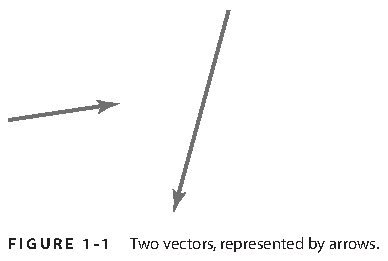
\includegraphics[width=0.92\linewidth,height=0.72\textheight,keepaspectratio]{../assets/figures/fig-1_1-p060.pdf}
\par{\footnotesize\bfseries Рисунок 1-1 (исходная стр. 60)}
\end{center}
\vspace{4bp}
\begin{center}
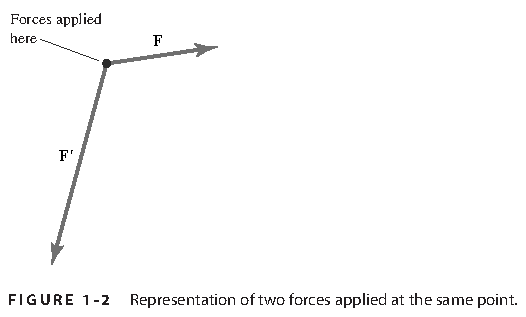
\includegraphics[width=0.92\linewidth,height=0.72\textheight,keepaspectratio]{../assets/figures/fig-1_2-p061.pdf}
\par{\footnotesize\bfseries Рисунок 1-2 (исходная стр. 61)}
\end{center}
\vspace{4bp}
\begin{center}
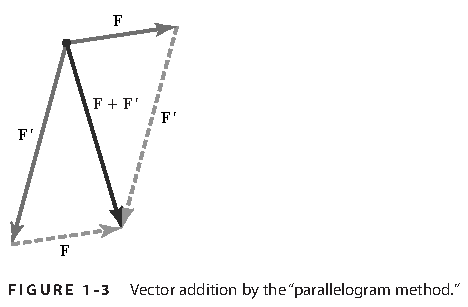
\includegraphics[width=0.92\linewidth,height=0.72\textheight,keepaspectratio]{../assets/figures/fig-1_3-p061.pdf}
\par{\footnotesize\bfseries Рисунок 1-3 (исходная стр. 61)}
\end{center}
\vspace{4bp}
\begin{center}
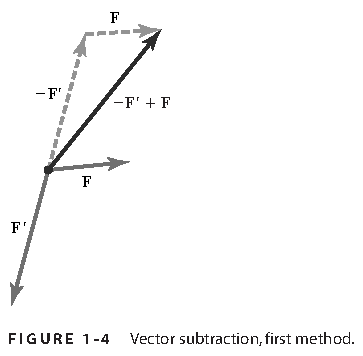
\includegraphics[width=0.92\linewidth,height=0.72\textheight,keepaspectratio]{../assets/figures/fig-1_4-p062.pdf}
\par{\footnotesize\bfseries Рисунок 1-4 (исходная стр. 62)}
\end{center}
\vspace{4bp}
\begin{center}
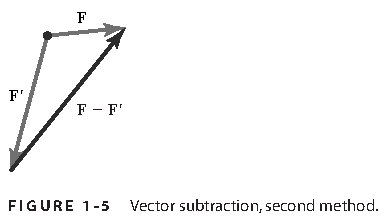
\includegraphics[width=0.92\linewidth,height=0.72\textheight,keepaspectratio]{../assets/figures/fig-1_5-p062.pdf}
\par{\footnotesize\bfseries Рисунок 1-5 (исходная стр. 62)}
\end{center}
\vspace{4bp}
\begin{center}
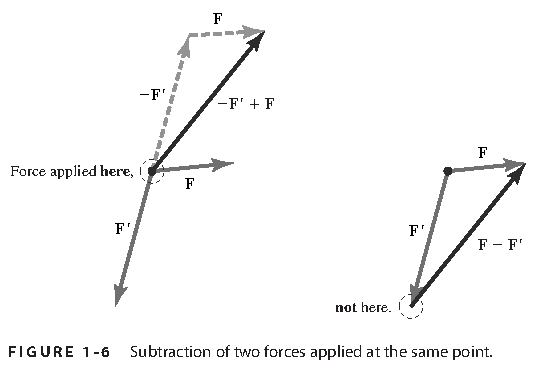
\includegraphics[width=0.92\linewidth,height=0.72\textheight,keepaspectratio]{../assets/figures/fig-1_6-p063.pdf}
\par{\footnotesize\bfseries Рисунок 1-6 (исходная стр. 63)}
\end{center}
\vspace{4bp}
\begin{center}
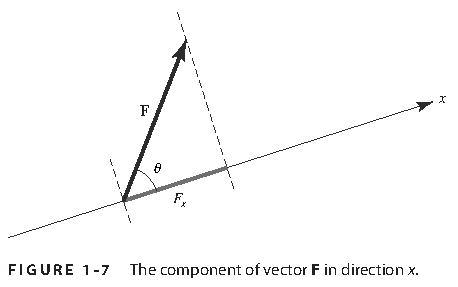
\includegraphics[width=0.92\linewidth,height=0.72\textheight,keepaspectratio]{../assets/figures/fig-1_7-p063.pdf}
\par{\footnotesize\bfseries Рисунок 1-7 (исходная стр. 63)}
\end{center}
\vspace{4bp}
\begin{center}
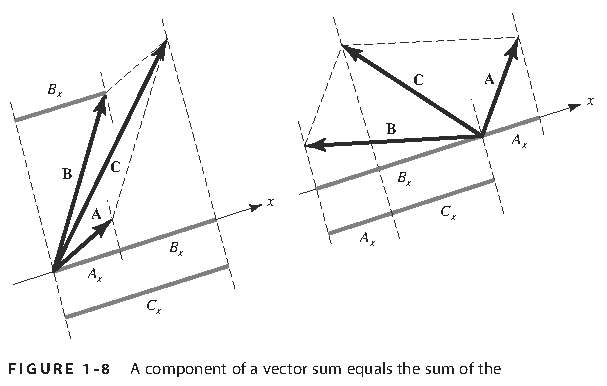
\includegraphics[width=0.92\linewidth,height=0.72\textheight,keepaspectratio]{../assets/figures/fig-1_8-p064.pdf}
\par{\footnotesize\bfseries Рисунок 1-8 (исходная стр. 64)}
\end{center}
\vspace{4bp}
\begin{center}
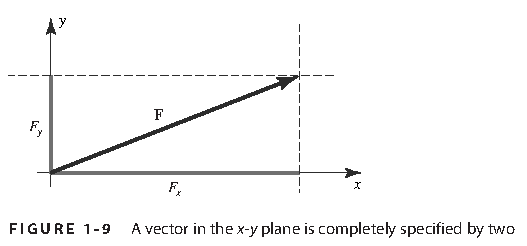
\includegraphics[width=0.92\linewidth,height=0.72\textheight,keepaspectratio]{../assets/figures/fig-1_9-p064.pdf}
\par{\footnotesize\bfseries Рисунок 1-9 (исходная стр. 64)}
\end{center}
\vspace{4bp}
\begin{center}
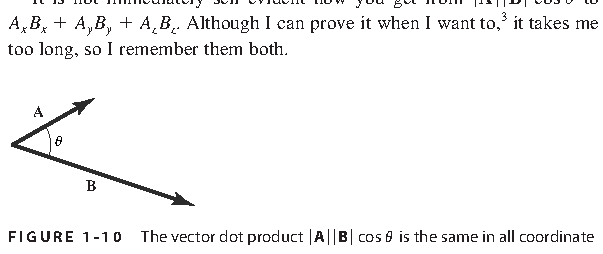
\includegraphics[width=0.92\linewidth,height=0.72\textheight,keepaspectratio]{../assets/figures/fig-1_10-p065.pdf}
\par{\footnotesize\bfseries Рисунок 1-10 (исходная стр. 65)}
\end{center}
\vspace{4bp}
\begin{center}
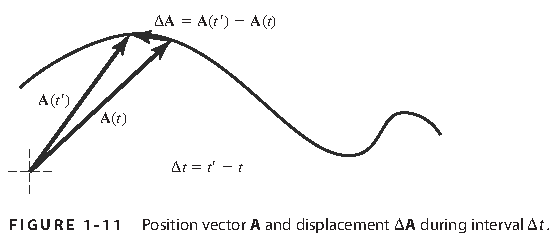
\includegraphics[width=0.92\linewidth,height=0.72\textheight,keepaspectratio]{../assets/figures/fig-1_11-p066.pdf}
\par{\footnotesize\bfseries Рисунок 1-11 (исходная стр. 66)}
\end{center}
\vspace{4bp}
\begin{center}
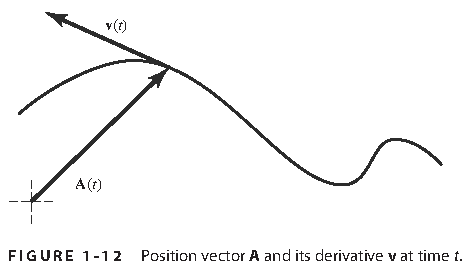
\includegraphics[width=0.92\linewidth,height=0.72\textheight,keepaspectratio]{../assets/figures/fig-1_12-p067.pdf}
\par{\footnotesize\bfseries Рисунок 1-12 (исходная стр. 67)}
\end{center}
\vspace{4bp}
\begin{center}
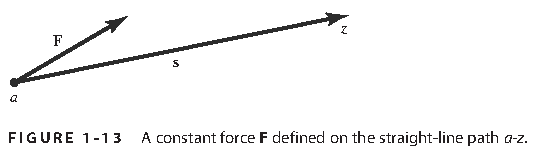
\includegraphics[width=0.92\linewidth,height=0.72\textheight,keepaspectratio]{../assets/figures/fig-1_13-p069.pdf}
\par{\footnotesize\bfseries Рисунок 1-13 (исходная стр. 69)}
\end{center}
\vspace{4bp}
\begin{center}
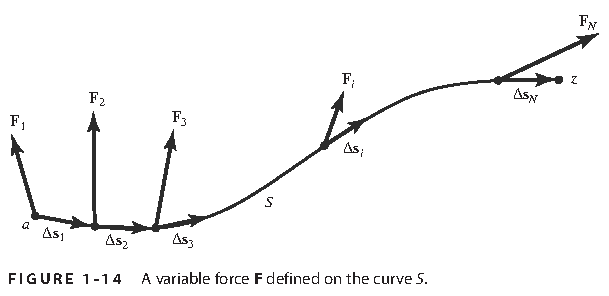
\includegraphics[width=0.92\linewidth,height=0.72\textheight,keepaspectratio]{../assets/figures/fig-1_14-p070.pdf}
\par{\footnotesize\bfseries Рисунок 1-14 (исходная стр. 70)}
\end{center}
\vspace{4bp}
\begin{center}
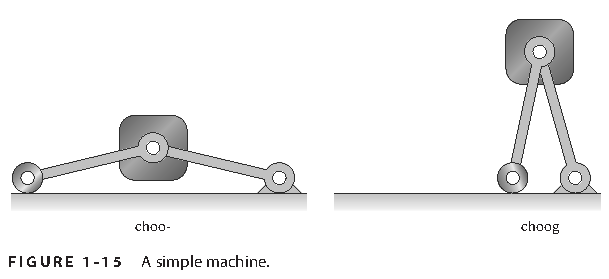
\includegraphics[width=0.92\linewidth,height=0.72\textheight,keepaspectratio]{../assets/figures/fig-1_15-p071.pdf}
\par{\footnotesize\bfseries Рисунок 1-15 (исходная стр. 71)}
\end{center}
\vspace{4bp}
\begin{center}
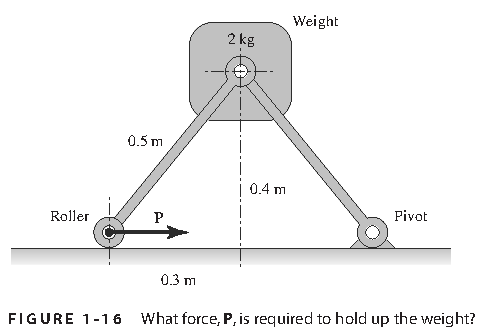
\includegraphics[width=0.92\linewidth,height=0.72\textheight,keepaspectratio]{../assets/figures/fig-1_16-p071.pdf}
\par{\footnotesize\bfseries Рисунок 1-16 (исходная стр. 71)}
\end{center}
\vspace{4bp}
\begin{center}
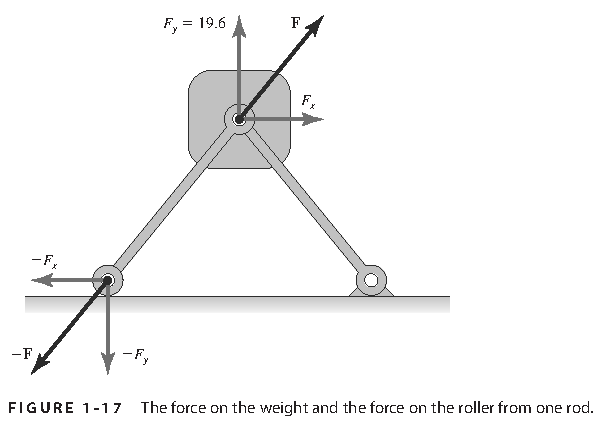
\includegraphics[width=0.92\linewidth,height=0.72\textheight,keepaspectratio]{../assets/figures/fig-1_17-p073.pdf}
\par{\footnotesize\bfseries Рисунок 1-17 (исходная стр. 73)}
\end{center}
\vspace{4bp}
\begin{center}
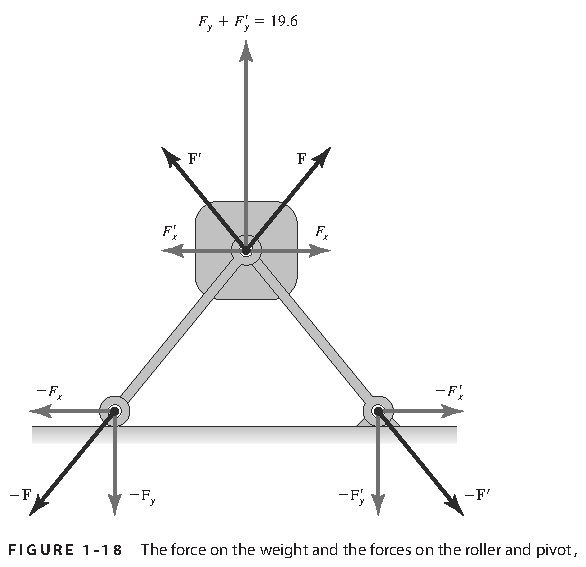
\includegraphics[width=0.92\linewidth,height=0.72\textheight,keepaspectratio]{../assets/figures/fig-1_18-p074.pdf}
\par{\footnotesize\bfseries Рисунок 1-18 (исходная стр. 74)}
\end{center}
\vspace{4bp}
\begin{center}
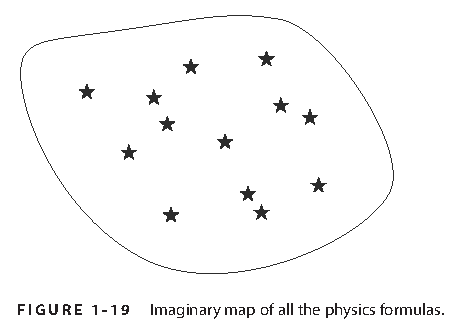
\includegraphics[width=0.92\linewidth,height=0.72\textheight,keepaspectratio]{../assets/figures/fig-1_19-p076.pdf}
\par{\footnotesize\bfseries Рисунок 1-19 (исходная стр. 76)}
\end{center}
\vspace{4bp}
\begin{center}
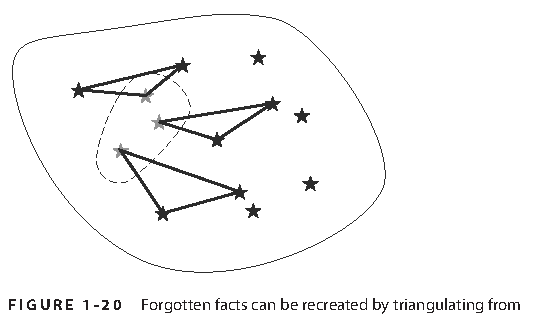
\includegraphics[width=0.92\linewidth,height=0.72\textheight,keepaspectratio]{../assets/figures/fig-1_20-p076.pdf}
\par{\footnotesize\bfseries Рисунок 1-20 (исходная стр. 76)}
\end{center}
\vspace{4bp}
\begin{center}
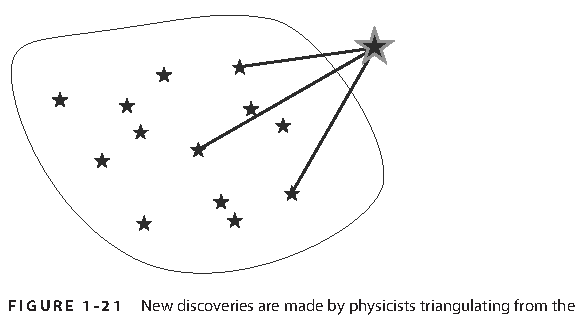
\includegraphics[width=0.92\linewidth,height=0.72\textheight,keepaspectratio]{../assets/figures/fig-1_21-p077.pdf}
\par{\footnotesize\bfseries Рисунок 1-21 (исходная стр. 77)}
\end{center}
\vspace{4bp}
\begin{center}
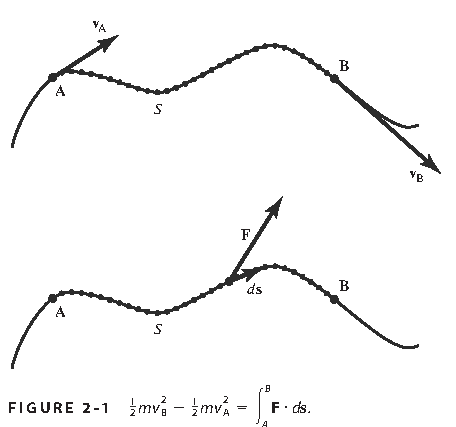
\includegraphics[width=0.92\linewidth,height=0.72\textheight,keepaspectratio]{../assets/figures/fig-2_112-p082.pdf}
\par{\footnotesize\bfseries Рисунок 2-112 (исходная стр. 82)}
\end{center}
\vspace{4bp}
\begin{center}
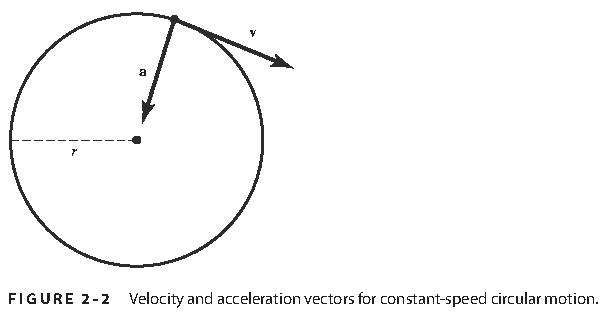
\includegraphics[width=0.92\linewidth,height=0.72\textheight,keepaspectratio]{../assets/figures/fig-2_2-p083.pdf}
\par{\footnotesize\bfseries Рисунок 2-2 (исходная стр. 83)}
\end{center}
\vspace{4bp}
\begin{center}
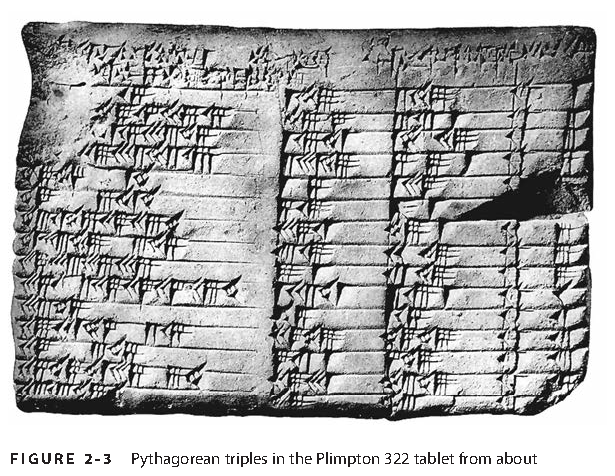
\includegraphics[width=0.92\linewidth,height=0.72\textheight,keepaspectratio]{../assets/figures/fig-2_3-p087.pdf}
\par{\footnotesize\bfseries Рисунок 2-3 (исходная стр. 87)}
\end{center}
\vspace{4bp}
\begin{center}
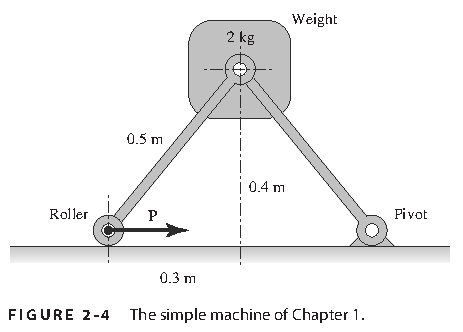
\includegraphics[width=0.92\linewidth,height=0.72\textheight,keepaspectratio]{../assets/figures/fig-2_4-p088.pdf}
\par{\footnotesize\bfseries Рисунок 2-4 (исходная стр. 88)}
\end{center}
\vspace{4bp}
\begin{center}
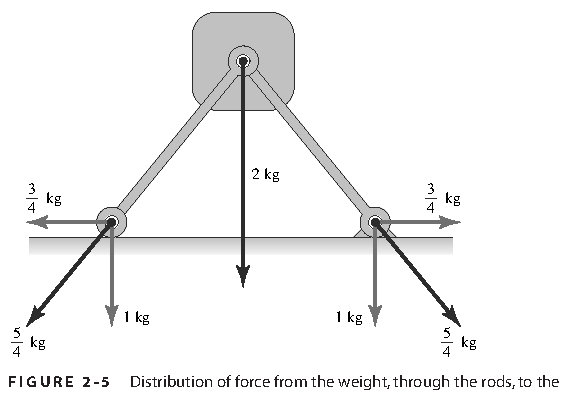
\includegraphics[width=0.92\linewidth,height=0.72\textheight,keepaspectratio]{../assets/figures/fig-2_5-p088.pdf}
\par{\footnotesize\bfseries Рисунок 2-5 (исходная стр. 88)}
\end{center}
\vspace{4bp}
\begin{center}
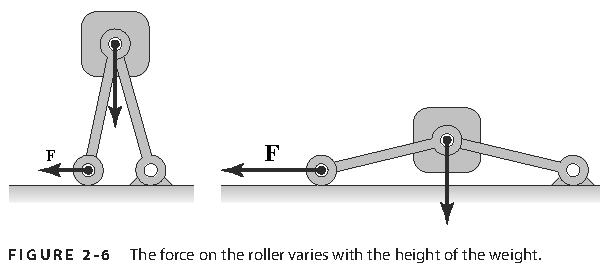
\includegraphics[width=0.92\linewidth,height=0.72\textheight,keepaspectratio]{../assets/figures/fig-2_6-p089.pdf}
\par{\footnotesize\bfseries Рисунок 2-6 (исходная стр. 89)}
\end{center}
\vspace{4bp}
\begin{center}
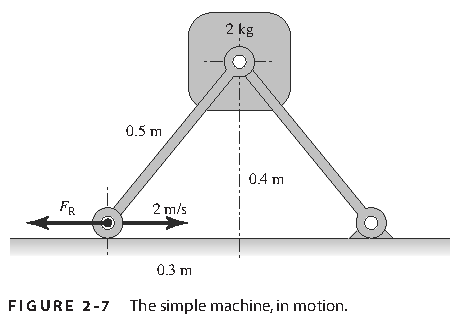
\includegraphics[width=0.92\linewidth,height=0.72\textheight,keepaspectratio]{../assets/figures/fig-2_7-p091.pdf}
\par{\footnotesize\bfseries Рисунок 2-7 (исходная стр. 91)}
\end{center}
\vspace{4bp}
\begin{center}
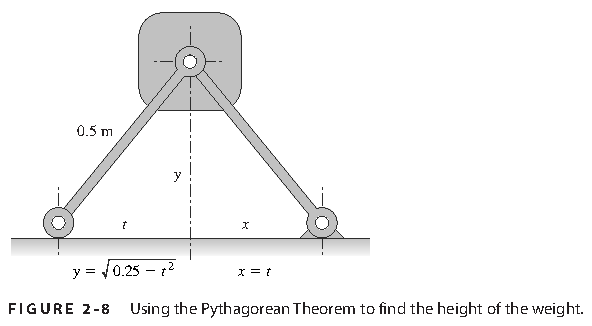
\includegraphics[width=0.92\linewidth,height=0.72\textheight,keepaspectratio]{../assets/figures/fig-2_8-p093.pdf}
\par{\footnotesize\bfseries Рисунок 2-8 (исходная стр. 93)}
\end{center}
\vspace{4bp}
\begin{center}
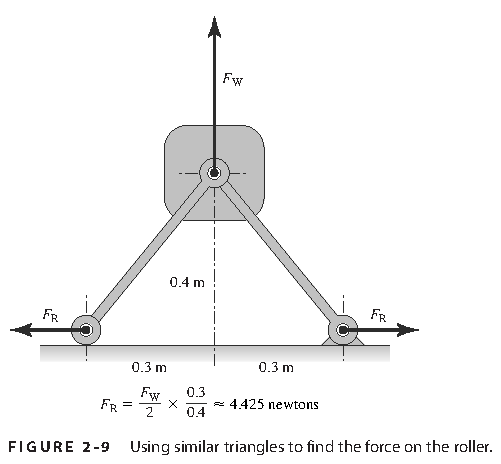
\includegraphics[width=0.92\linewidth,height=0.72\textheight,keepaspectratio]{../assets/figures/fig-2_9-p095.pdf}
\par{\footnotesize\bfseries Рисунок 2-9 (исходная стр. 95)}
\end{center}
\vspace{4bp}
\begin{center}
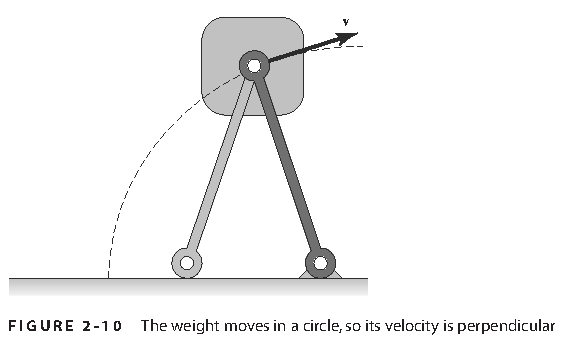
\includegraphics[width=0.92\linewidth,height=0.72\textheight,keepaspectratio]{../assets/figures/fig-2_10-p098.pdf}
\par{\footnotesize\bfseries Рисунок 2-10 (исходная стр. 98)}
\end{center}
\vspace{4bp}
\begin{center}
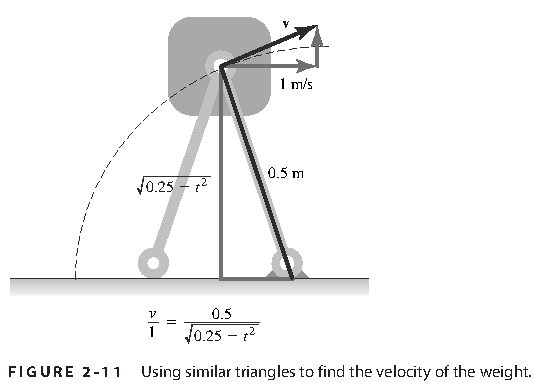
\includegraphics[width=0.92\linewidth,height=0.72\textheight,keepaspectratio]{../assets/figures/fig-2_11-p099.pdf}
\par{\footnotesize\bfseries Рисунок 2-11 (исходная стр. 99)}
\end{center}
\vspace{4bp}
\begin{center}
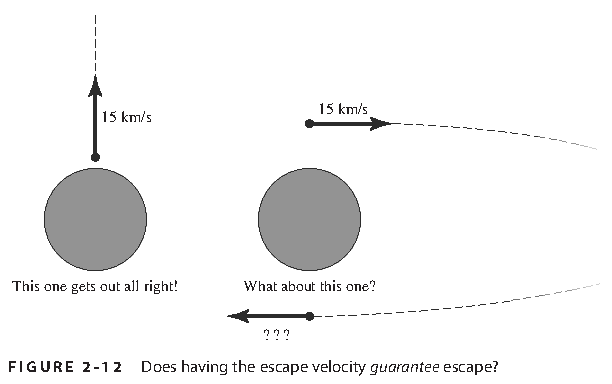
\includegraphics[width=0.92\linewidth,height=0.72\textheight,keepaspectratio]{../assets/figures/fig-2_12-p102.pdf}
\par{\footnotesize\bfseries Рисунок 2-12 (исходная стр. 102)}
\end{center}
\vspace{4bp}
\begin{center}
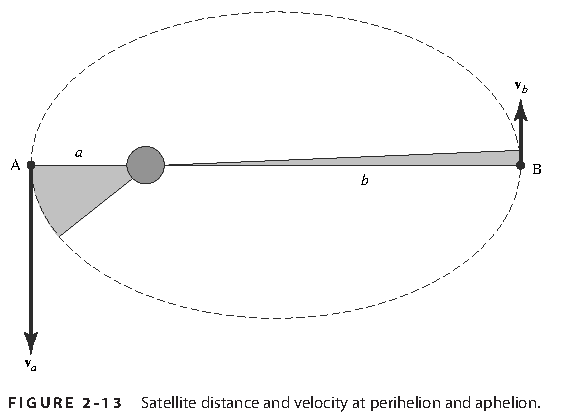
\includegraphics[width=0.92\linewidth,height=0.72\textheight,keepaspectratio]{../assets/figures/fig-2_13-p103.pdf}
\par{\footnotesize\bfseries Рисунок 2-13 (исходная стр. 103)}
\end{center}
\vspace{4bp}
\begin{center}
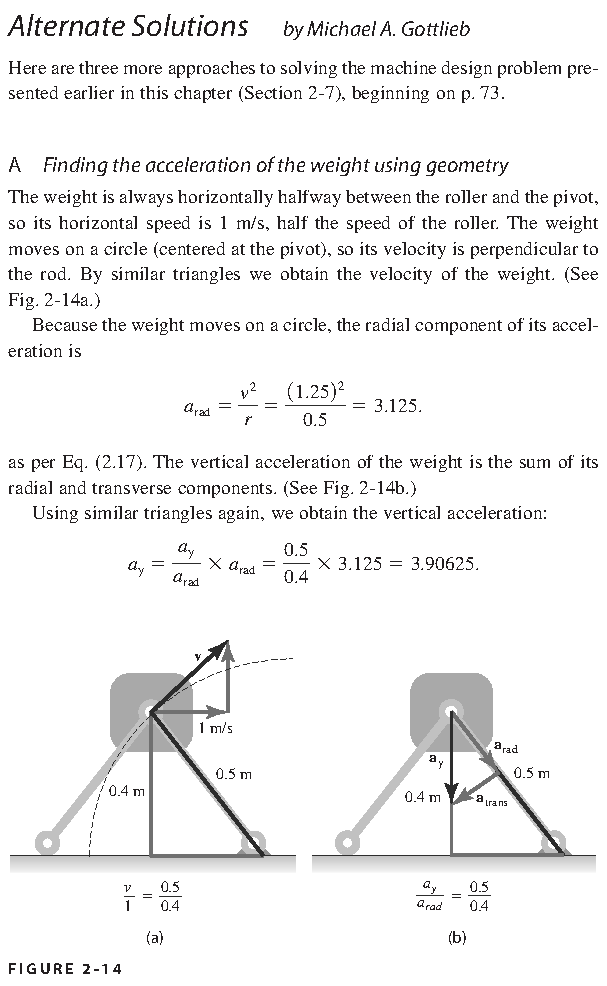
\includegraphics[width=0.92\linewidth,height=0.72\textheight,keepaspectratio]{../assets/figures/fig-2_14-p104.pdf}
\par{\footnotesize\bfseries Рисунок 2-14 (исходная стр. 104)}
\end{center}
\vspace{4bp}
\begin{center}
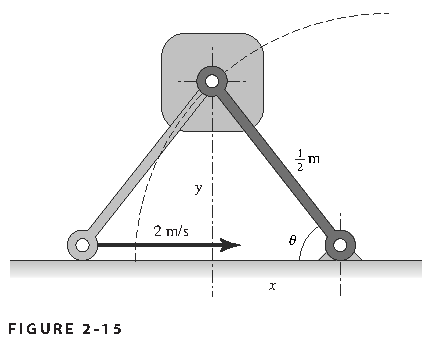
\includegraphics[width=0.92\linewidth,height=0.72\textheight,keepaspectratio]{../assets/figures/fig-2_15-p105.pdf}
\par{\footnotesize\bfseries Рисунок 2-15 (исходная стр. 105)}
\end{center}
\vspace{4bp}
\begin{center}
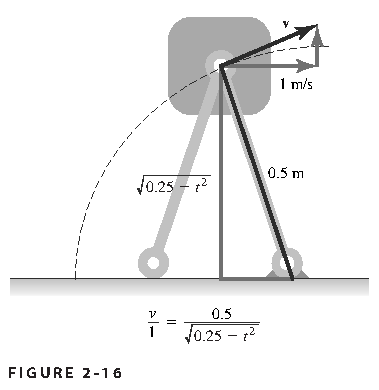
\includegraphics[width=0.92\linewidth,height=0.72\textheight,keepaspectratio]{../assets/figures/fig-2_16-p106.pdf}
\par{\footnotesize\bfseries Рисунок 2-16 (исходная стр. 106)}
\end{center}
\vspace{4bp}
\begin{center}
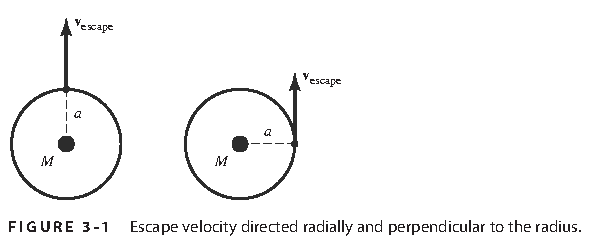
\includegraphics[width=0.92\linewidth,height=0.72\textheight,keepaspectratio]{../assets/figures/fig-3_1-p108.pdf}
\par{\footnotesize\bfseries Рисунок 3-1 (исходная стр. 108)}
\end{center}
\vspace{4bp}
\begin{center}
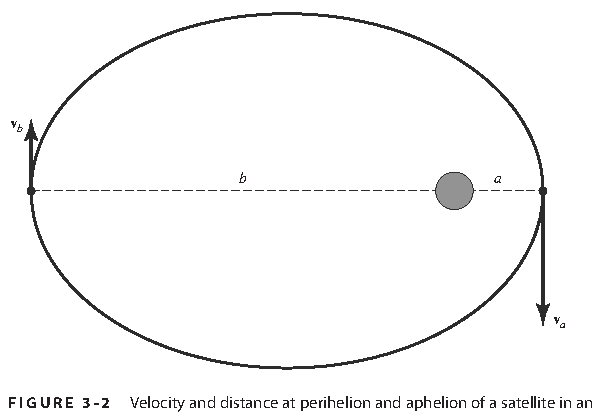
\includegraphics[width=0.92\linewidth,height=0.72\textheight,keepaspectratio]{../assets/figures/fig-3_2-p109.pdf}
\par{\footnotesize\bfseries Рисунок 3-2 (исходная стр. 109)}
\end{center}
\vspace{4bp}
\begin{center}
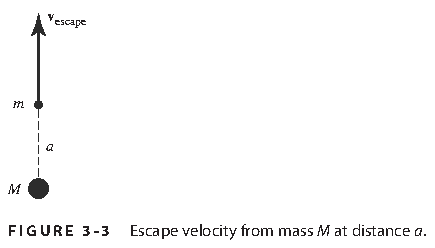
\includegraphics[width=0.92\linewidth,height=0.72\textheight,keepaspectratio]{../assets/figures/fig-3_3-p109.pdf}
\par{\footnotesize\bfseries Рисунок 3-3 (исходная стр. 109)}
\end{center}
\vspace{4bp}
\begin{center}
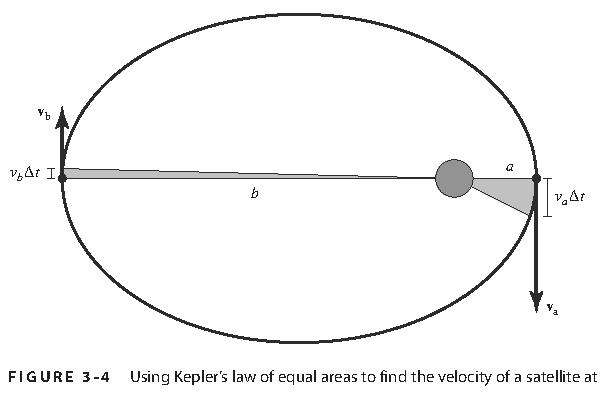
\includegraphics[width=0.92\linewidth,height=0.72\textheight,keepaspectratio]{../assets/figures/fig-3_4-p111.pdf}
\par{\footnotesize\bfseries Рисунок 3-4 (исходная стр. 111)}
\end{center}
\vspace{4bp}
\begin{center}
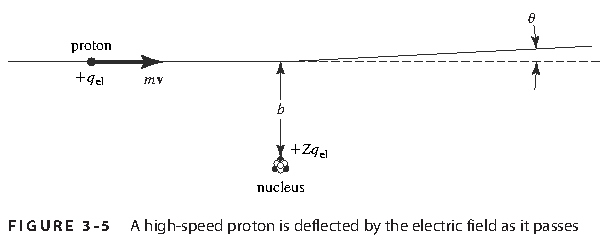
\includegraphics[width=0.92\linewidth,height=0.72\textheight,keepaspectratio]{../assets/figures/fig-3_5-p113.pdf}
\par{\footnotesize\bfseries Рисунок 3-5 (исходная стр. 113)}
\end{center}
\vspace{4bp}
\begin{center}
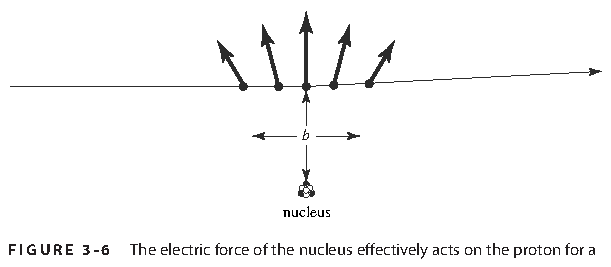
\includegraphics[width=0.92\linewidth,height=0.72\textheight,keepaspectratio]{../assets/figures/fig-3_6-p114.pdf}
\par{\footnotesize\bfseries Рисунок 3-6 (исходная стр. 114)}
\end{center}
\vspace{4bp}
\begin{center}
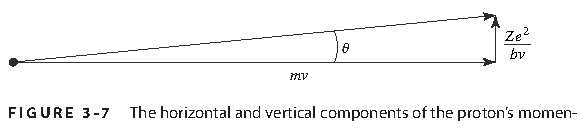
\includegraphics[width=0.92\linewidth,height=0.72\textheight,keepaspectratio]{../assets/figures/fig-3_7-p115.pdf}
\par{\footnotesize\bfseries Рисунок 3-7 (исходная стр. 115)}
\end{center}
\vspace{4bp}
\begin{center}
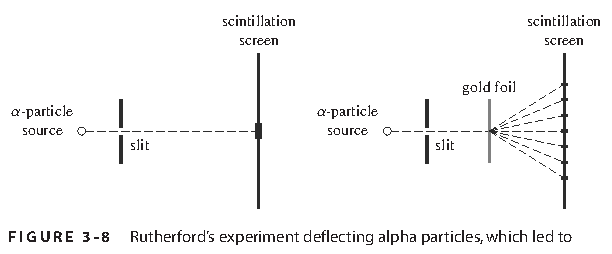
\includegraphics[width=0.92\linewidth,height=0.72\textheight,keepaspectratio]{../assets/figures/fig-3_8-p116.pdf}
\par{\footnotesize\bfseries Рисунок 3-8 (исходная стр. 116)}
\end{center}
\vspace{4bp}
\begin{center}
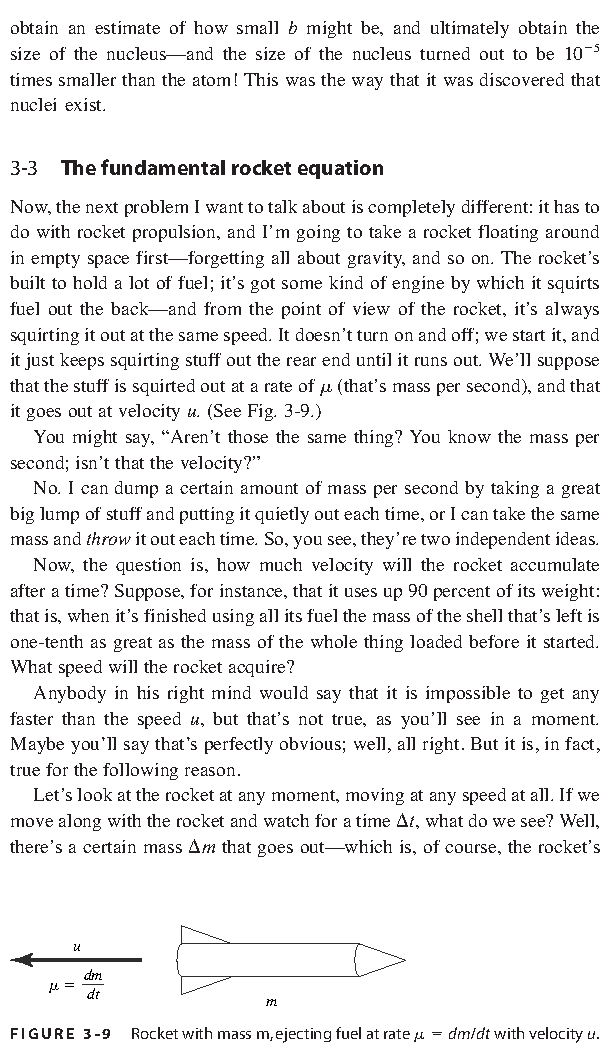
\includegraphics[width=0.92\linewidth,height=0.72\textheight,keepaspectratio]{../assets/figures/fig-3_9-p117.pdf}
\par{\footnotesize\bfseries Рисунок 3-9 (исходная стр. 117)}
\end{center}
\vspace{4bp}
\begin{center}
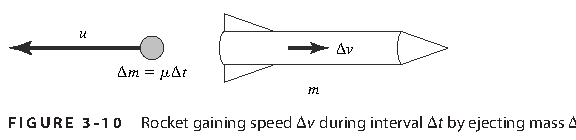
\includegraphics[width=0.92\linewidth,height=0.72\textheight,keepaspectratio]{../assets/figures/fig-3_10-p118.pdf}
\par{\footnotesize\bfseries Рисунок 3-10 (исходная стр. 118)}
\end{center}
\vspace{4bp}
\begin{center}
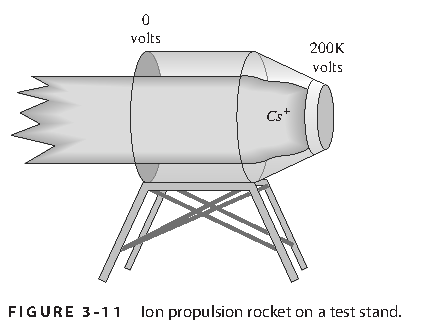
\includegraphics[width=0.92\linewidth,height=0.72\textheight,keepaspectratio]{../assets/figures/fig-3_11-p122.pdf}
\par{\footnotesize\bfseries Рисунок 3-11 (исходная стр. 122)}
\end{center}
\vspace{4bp}
\begin{center}
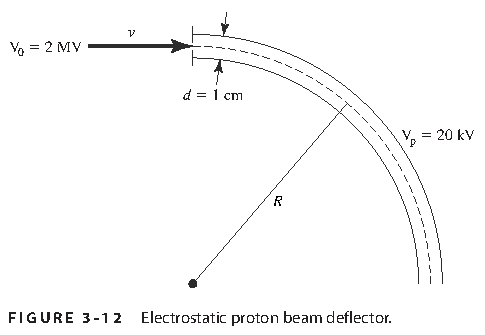
\includegraphics[width=0.92\linewidth,height=0.72\textheight,keepaspectratio]{../assets/figures/fig-3_12-p126.pdf}
\par{\footnotesize\bfseries Рисунок 3-12 (исходная стр. 126)}
\end{center}
\vspace{4bp}
\begin{center}
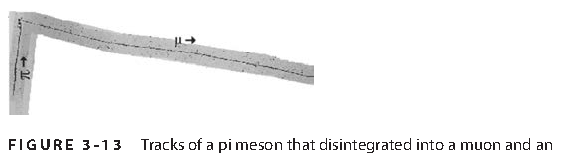
\includegraphics[width=0.92\linewidth,height=0.72\textheight,keepaspectratio]{../assets/figures/fig-3_13-p129.pdf}
\par{\footnotesize\bfseries Рисунок 3-13 (исходная стр. 129)}
\end{center}
\vspace{4bp}
\begin{center}
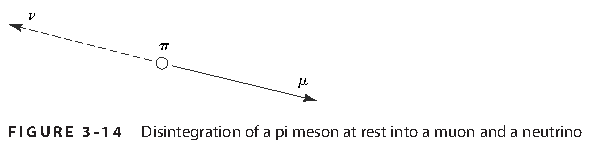
\includegraphics[width=0.92\linewidth,height=0.72\textheight,keepaspectratio]{../assets/figures/fig-3_14-p129.pdf}
\par{\footnotesize\bfseries Рисунок 3-14 (исходная стр. 129)}
\end{center}
\vspace{4bp}
\begin{center}
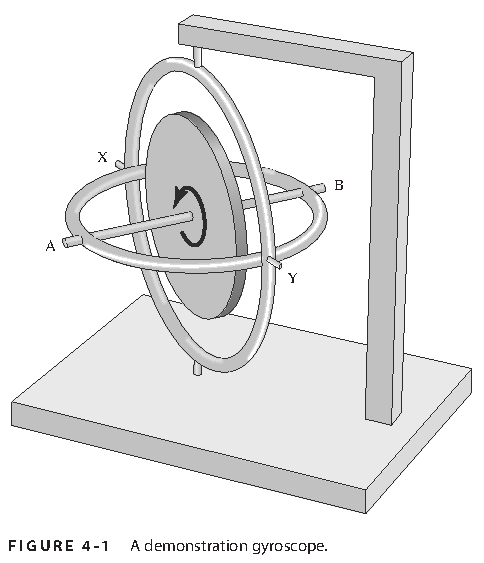
\includegraphics[width=0.92\linewidth,height=0.72\textheight,keepaspectratio]{../assets/figures/fig-4_1-p133.pdf}
\par{\footnotesize\bfseries Рисунок 4-1 (исходная стр. 133)}
\end{center}
\vspace{4bp}
\begin{center}
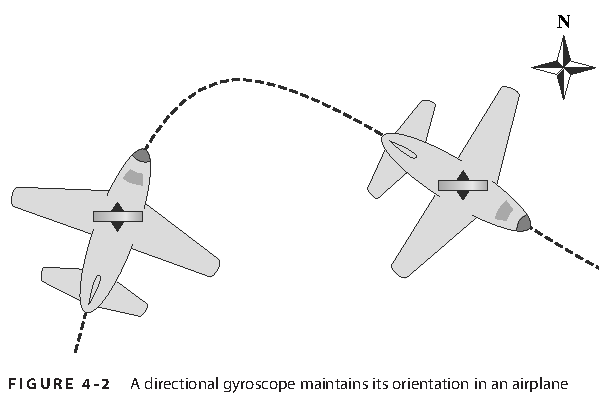
\includegraphics[width=0.92\linewidth,height=0.72\textheight,keepaspectratio]{../assets/figures/fig-4_2-p134.pdf}
\par{\footnotesize\bfseries Рисунок 4-2 (исходная стр. 134)}
\end{center}
\vspace{4bp}
\begin{center}
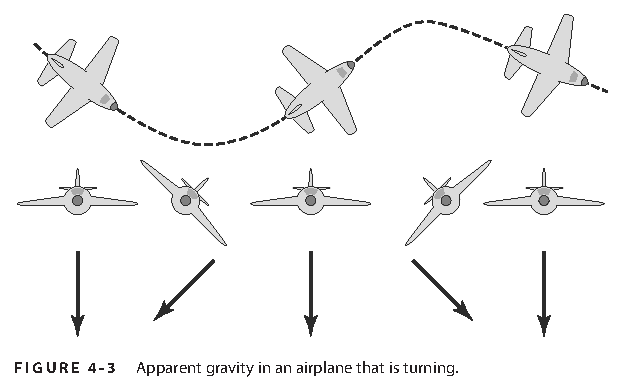
\includegraphics[width=0.92\linewidth,height=0.72\textheight,keepaspectratio]{../assets/figures/fig-4_3-p136.pdf}
\par{\footnotesize\bfseries Рисунок 4-3 (исходная стр. 136)}
\end{center}
\vspace{4bp}
\begin{center}
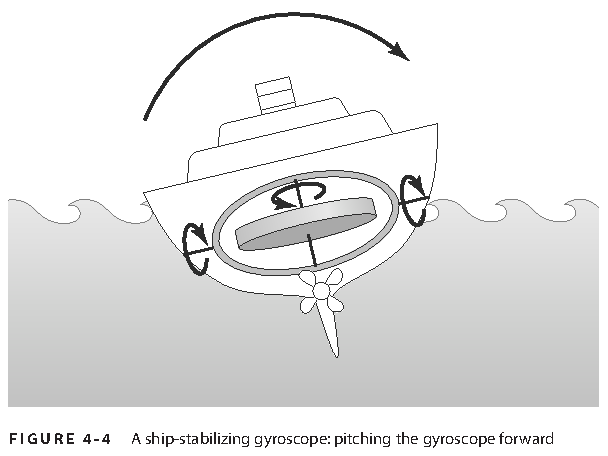
\includegraphics[width=0.92\linewidth,height=0.72\textheight,keepaspectratio]{../assets/figures/fig-4_4-p137.pdf}
\par{\footnotesize\bfseries Рисунок 4-4 (исходная стр. 137)}
\end{center}
\vspace{4bp}
\begin{center}
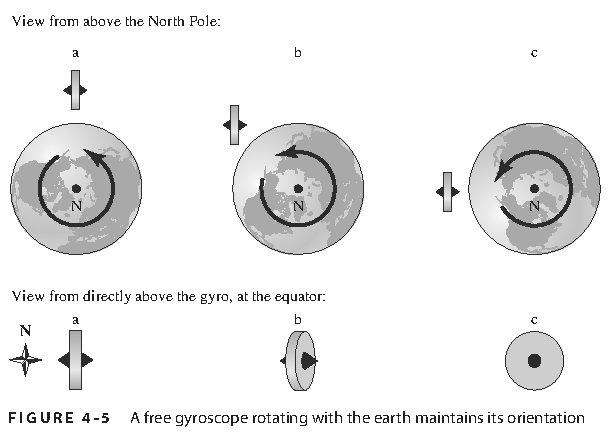
\includegraphics[width=0.92\linewidth,height=0.72\textheight,keepaspectratio]{../assets/figures/fig-4_5-p138.pdf}
\par{\footnotesize\bfseries Рисунок 4-5 (исходная стр. 138)}
\end{center}
\vspace{4bp}
\begin{center}
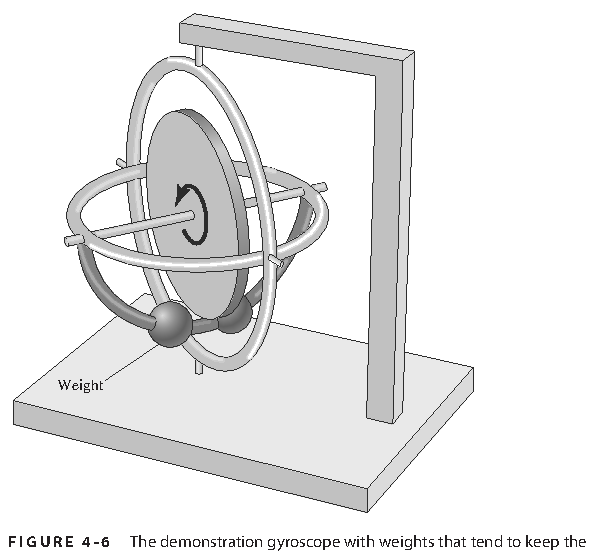
\includegraphics[width=0.92\linewidth,height=0.72\textheight,keepaspectratio]{../assets/figures/fig-4_6-p139.pdf}
\par{\footnotesize\bfseries Рисунок 4-6 (исходная стр. 139)}
\end{center}
\vspace{4bp}
\begin{center}
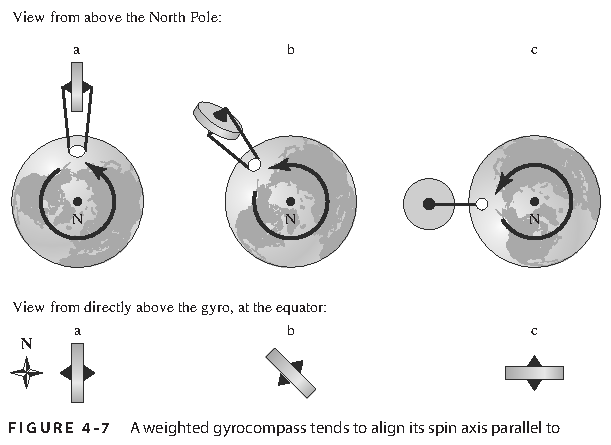
\includegraphics[width=0.92\linewidth,height=0.72\textheight,keepaspectratio]{../assets/figures/fig-4_7-p139.pdf}
\par{\footnotesize\bfseries Рисунок 4-7 (исходная стр. 139)}
\end{center}
\vspace{4bp}
\begin{center}
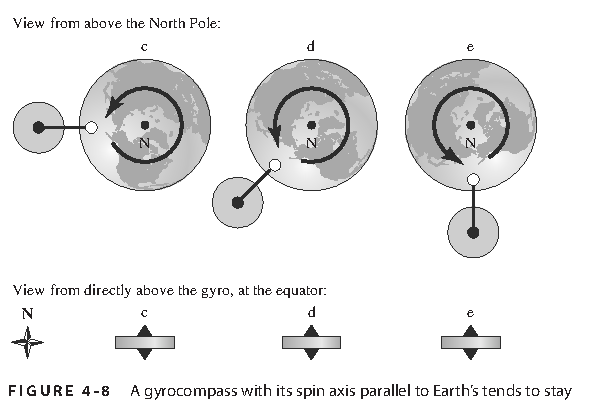
\includegraphics[width=0.92\linewidth,height=0.72\textheight,keepaspectratio]{../assets/figures/fig-4_8-p140.pdf}
\par{\footnotesize\bfseries Рисунок 4-8 (исходная стр. 140)}
\end{center}
\vspace{4bp}
\begin{center}
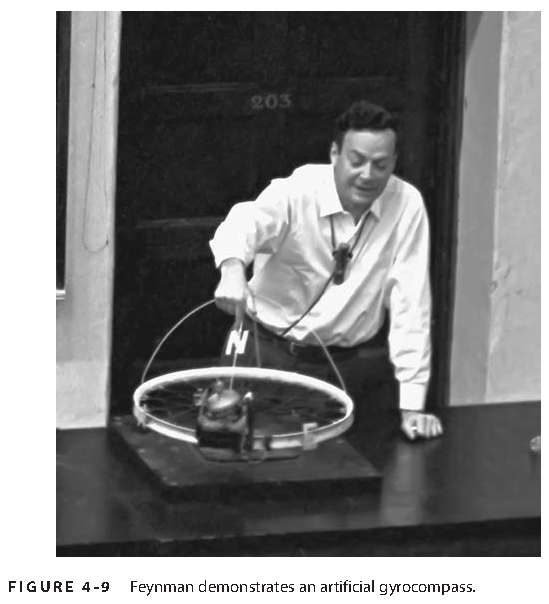
\includegraphics[width=0.92\linewidth,height=0.72\textheight,keepaspectratio]{../assets/figures/fig-4_9-p141.pdf}
\par{\footnotesize\bfseries Рисунок 4-9 (исходная стр. 141)}
\end{center}
\vspace{4bp}
\begin{center}
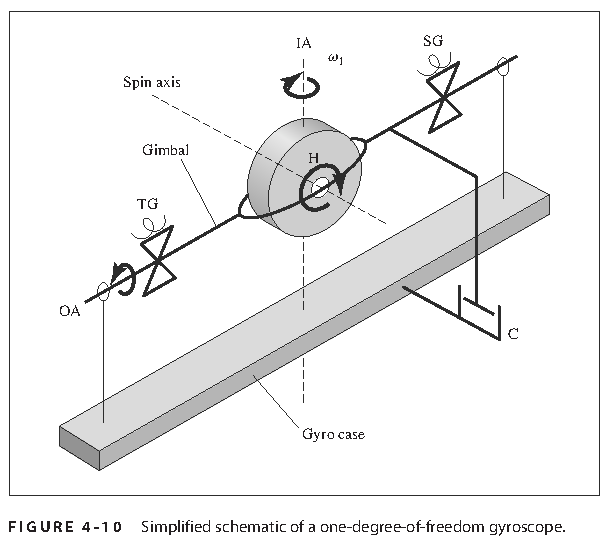
\includegraphics[width=0.92\linewidth,height=0.72\textheight,keepaspectratio]{../assets/figures/fig-4_10-p142.pdf}
\par{\footnotesize\bfseries Рисунок 4-10 (исходная стр. 142)}
\end{center}
\vspace{4bp}
\begin{center}
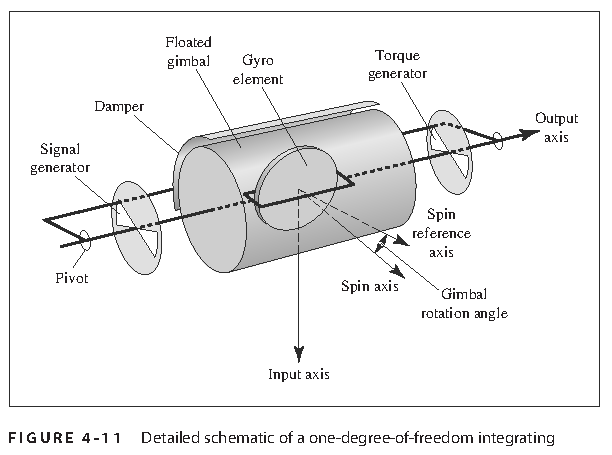
\includegraphics[width=0.92\linewidth,height=0.72\textheight,keepaspectratio]{../assets/figures/fig-4_11-p143.pdf}
\par{\footnotesize\bfseries Рисунок 4-11 (исходная стр. 143)}
\end{center}
\vspace{4bp}
\begin{center}
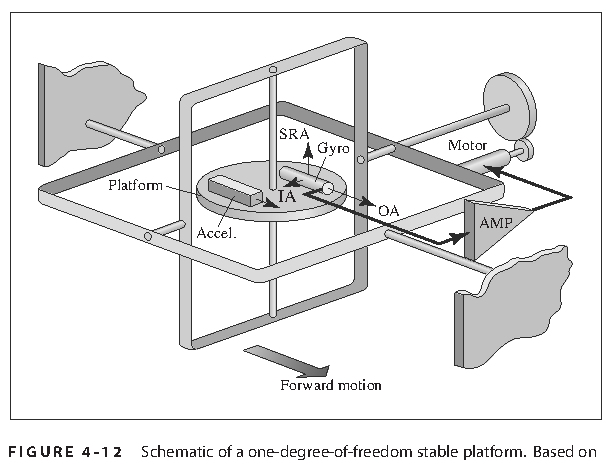
\includegraphics[width=0.92\linewidth,height=0.72\textheight,keepaspectratio]{../assets/figures/fig-4_12-p144.pdf}
\par{\footnotesize\bfseries Рисунок 4-12 (исходная стр. 144)}
\end{center}
\vspace{4bp}
\begin{center}
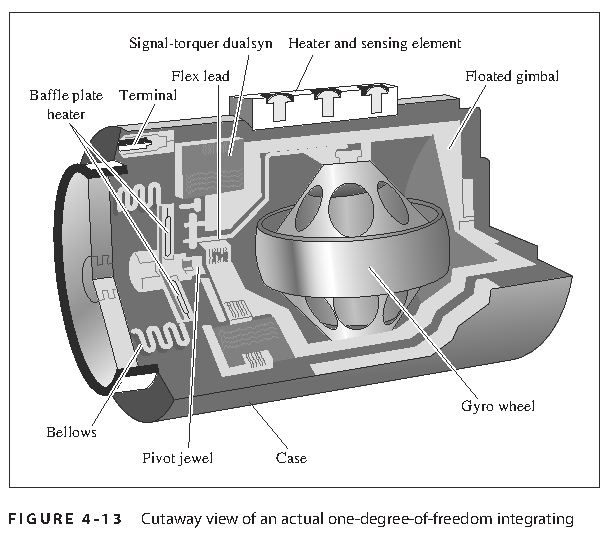
\includegraphics[width=0.92\linewidth,height=0.72\textheight,keepaspectratio]{../assets/figures/fig-4_13-p145.pdf}
\par{\footnotesize\bfseries Рисунок 4-13 (исходная стр. 145)}
\end{center}
\vspace{4bp}
\begin{center}
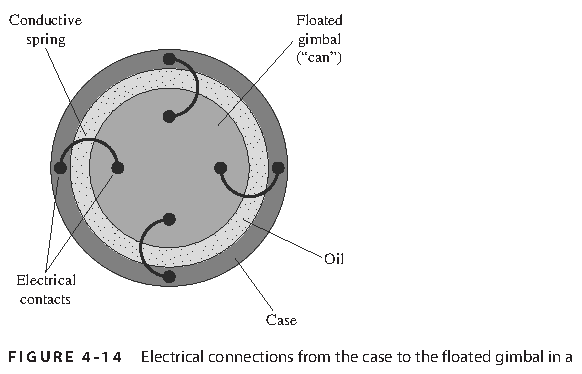
\includegraphics[width=0.92\linewidth,height=0.72\textheight,keepaspectratio]{../assets/figures/fig-4_14-p146.pdf}
\par{\footnotesize\bfseries Рисунок 4-14 (исходная стр. 146)}
\end{center}
\vspace{4bp}
\begin{center}
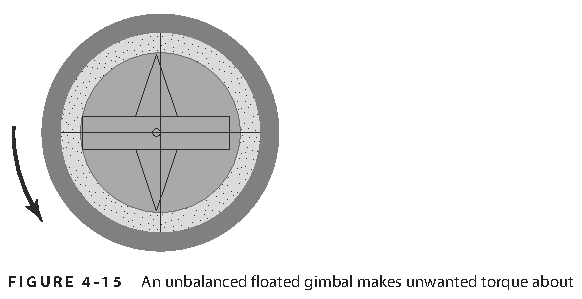
\includegraphics[width=0.92\linewidth,height=0.72\textheight,keepaspectratio]{../assets/figures/fig-4_15-p147.pdf}
\par{\footnotesize\bfseries Рисунок 4-15 (исходная стр. 147)}
\end{center}
\vspace{4bp}
\begin{center}
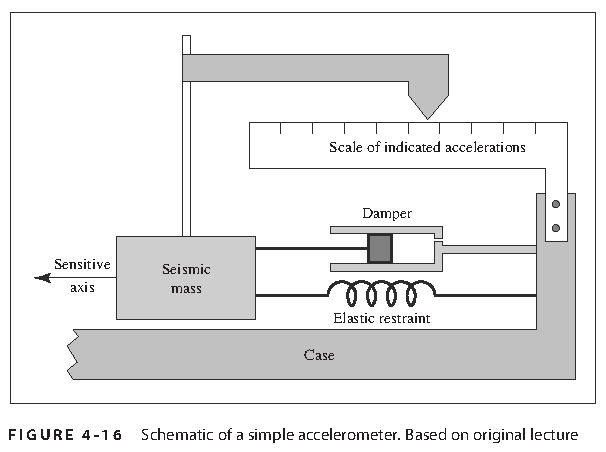
\includegraphics[width=0.92\linewidth,height=0.72\textheight,keepaspectratio]{../assets/figures/fig-4_16-p149.pdf}
\par{\footnotesize\bfseries Рисунок 4-16 (исходная стр. 149)}
\end{center}
\vspace{4bp}
\begin{center}
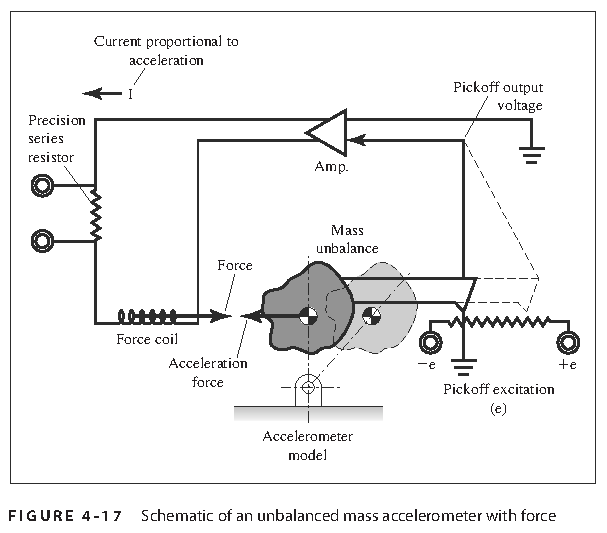
\includegraphics[width=0.92\linewidth,height=0.72\textheight,keepaspectratio]{../assets/figures/fig-4_17-p150.pdf}
\par{\footnotesize\bfseries Рисунок 4-17 (исходная стр. 150)}
\end{center}
\vspace{4bp}
\begin{center}
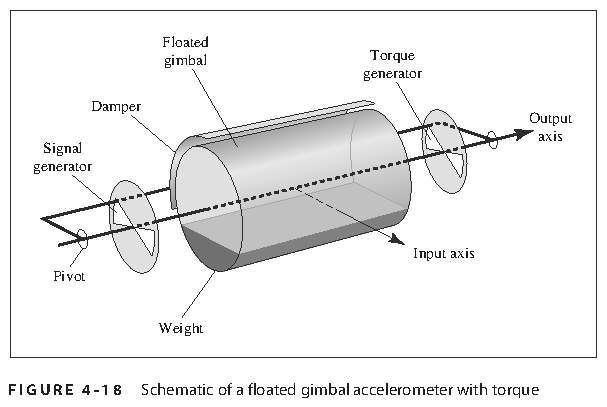
\includegraphics[width=0.92\linewidth,height=0.72\textheight,keepaspectratio]{../assets/figures/fig-4_18-p150.pdf}
\par{\footnotesize\bfseries Рисунок 4-18 (исходная стр. 150)}
\end{center}
\vspace{4bp}
\begin{center}
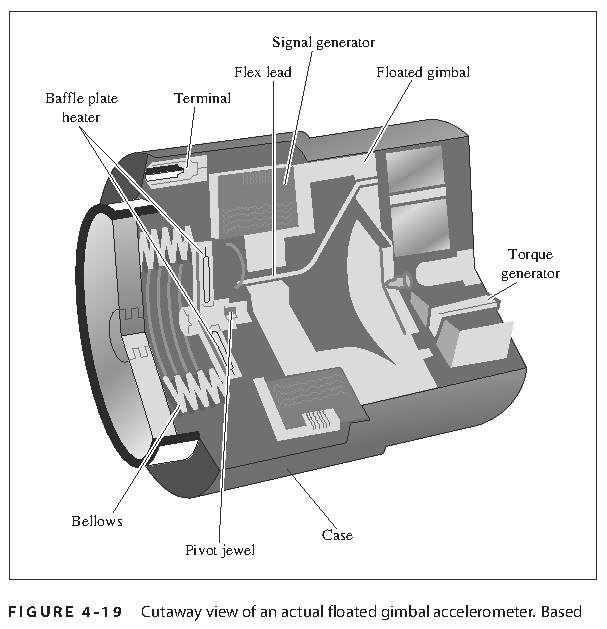
\includegraphics[width=0.92\linewidth,height=0.72\textheight,keepaspectratio]{../assets/figures/fig-4_19-p151.pdf}
\par{\footnotesize\bfseries Рисунок 4-19 (исходная стр. 151)}
\end{center}
\vspace{4bp}
\begin{center}
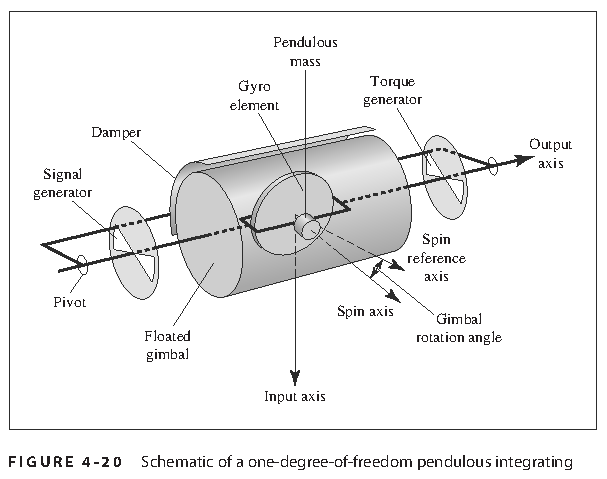
\includegraphics[width=0.92\linewidth,height=0.72\textheight,keepaspectratio]{../assets/figures/fig-4_20-p152.pdf}
\par{\footnotesize\bfseries Рисунок 4-20 (исходная стр. 152)}
\end{center}
\vspace{4bp}
\begin{center}
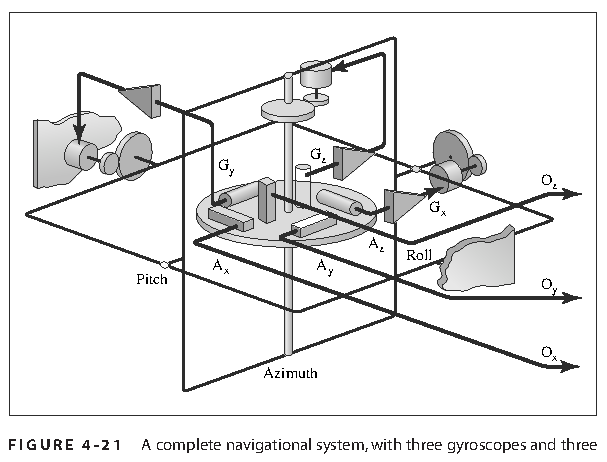
\includegraphics[width=0.92\linewidth,height=0.72\textheight,keepaspectratio]{../assets/figures/fig-4_21-p153.pdf}
\par{\footnotesize\bfseries Рисунок 4-21 (исходная стр. 153)}
\end{center}
\vspace{4bp}
\begin{center}
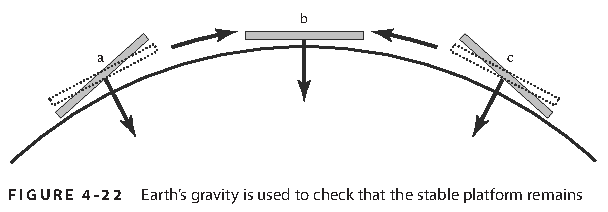
\includegraphics[width=0.92\linewidth,height=0.72\textheight,keepaspectratio]{../assets/figures/fig-4_22-p154.pdf}
\par{\footnotesize\bfseries Рисунок 4-22 (исходная стр. 154)}
\end{center}
\vspace{4bp}
\begin{center}
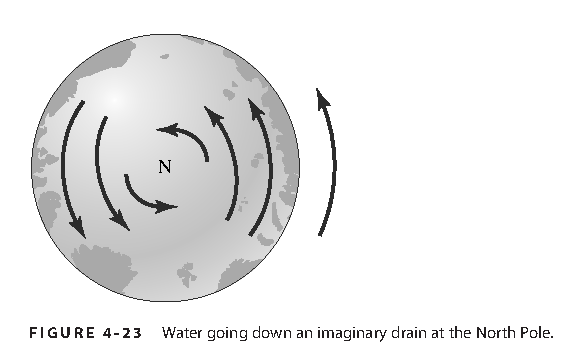
\includegraphics[width=0.92\linewidth,height=0.72\textheight,keepaspectratio]{../assets/figures/fig-4_23-p156.pdf}
\par{\footnotesize\bfseries Рисунок 4-23 (исходная стр. 156)}
\end{center}
\vspace{4bp}
\begin{center}
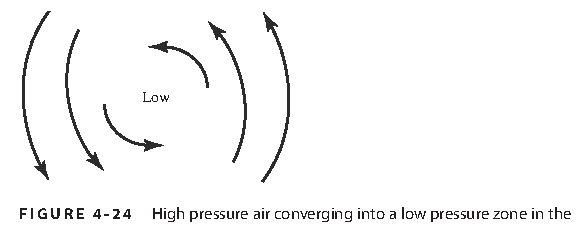
\includegraphics[width=0.92\linewidth,height=0.72\textheight,keepaspectratio]{../assets/figures/fig-4_24-p157.pdf}
\par{\footnotesize\bfseries Рисунок 4-24 (исходная стр. 157)}
\end{center}
\vspace{4bp}
\begin{center}
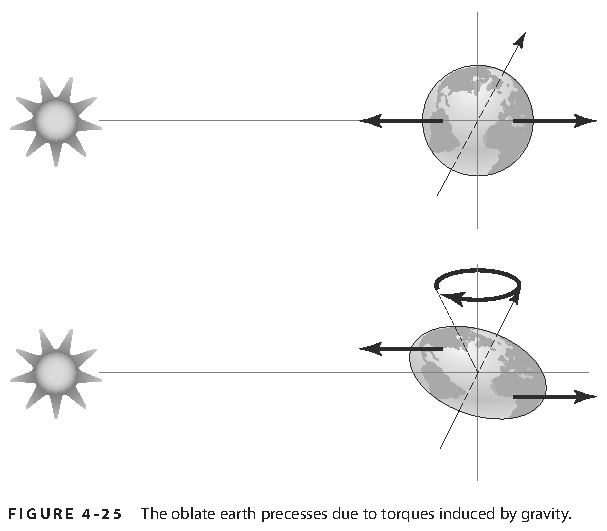
\includegraphics[width=0.92\linewidth,height=0.72\textheight,keepaspectratio]{../assets/figures/fig-4_25-p158.pdf}
\par{\footnotesize\bfseries Рисунок 4-25 (исходная стр. 158)}
\end{center}
\vspace{4bp}
\begin{center}
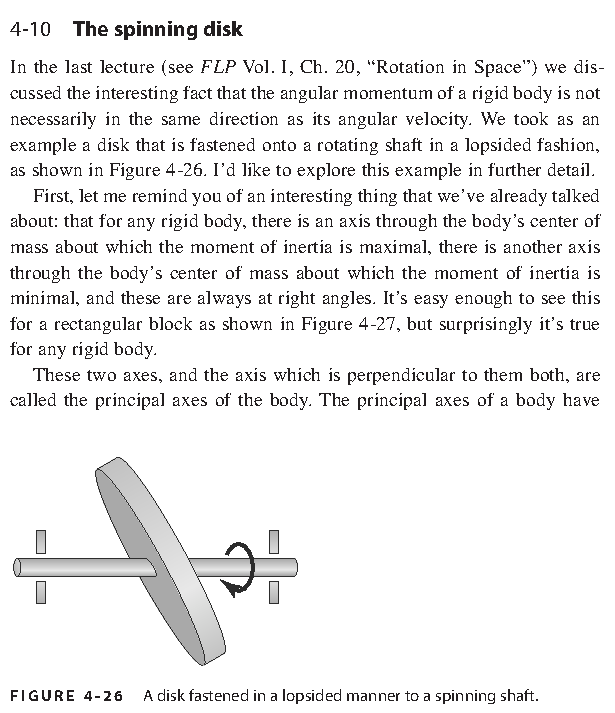
\includegraphics[width=0.92\linewidth,height=0.72\textheight,keepaspectratio]{../assets/figures/fig-4_26-p159.pdf}
\par{\footnotesize\bfseries Рисунок 4-26 (исходная стр. 159)}
\end{center}
\vspace{4bp}
\begin{center}
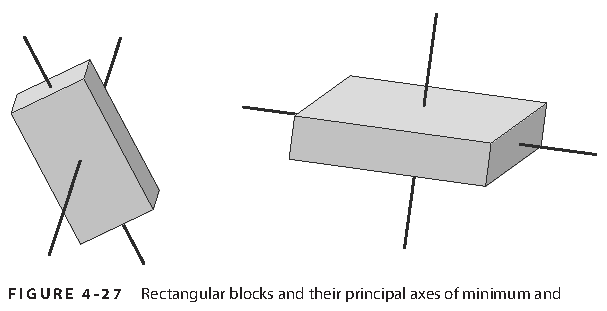
\includegraphics[width=0.92\linewidth,height=0.72\textheight,keepaspectratio]{../assets/figures/fig-4_27-p159.pdf}
\par{\footnotesize\bfseries Рисунок 4-27 (исходная стр. 159)}
\end{center}
\vspace{4bp}
\begin{center}
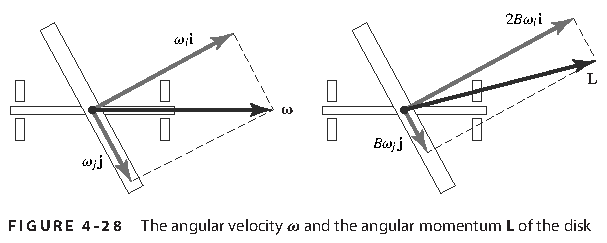
\includegraphics[width=0.92\linewidth,height=0.72\textheight,keepaspectratio]{../assets/figures/fig-4_28-p160.pdf}
\par{\footnotesize\bfseries Рисунок 4-28 (исходная стр. 160)}
\end{center}
\vspace{4bp}
\begin{center}
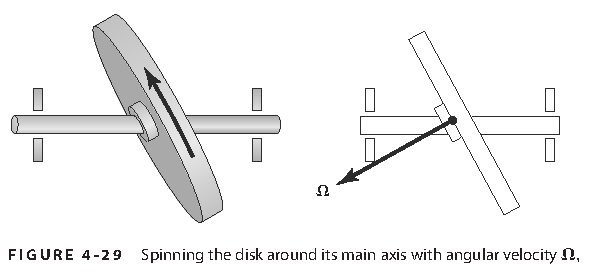
\includegraphics[width=0.92\linewidth,height=0.72\textheight,keepaspectratio]{../assets/figures/fig-4_29-p161.pdf}
\par{\footnotesize\bfseries Рисунок 4-29 (исходная стр. 161)}
\end{center}
\vspace{4bp}
\begin{center}
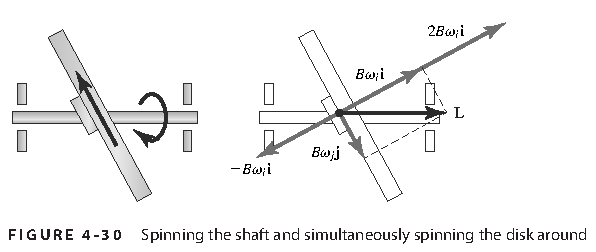
\includegraphics[width=0.92\linewidth,height=0.72\textheight,keepaspectratio]{../assets/figures/fig-4_30-p161.pdf}
\par{\footnotesize\bfseries Рисунок 4-30 (исходная стр. 161)}
\end{center}
\vspace{4bp}
\begin{center}
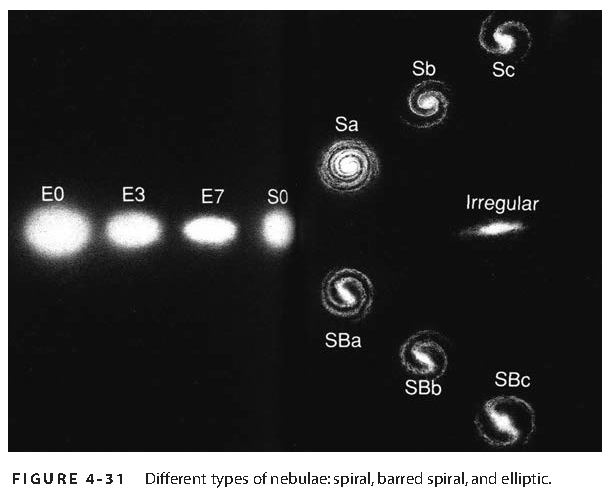
\includegraphics[width=0.92\linewidth,height=0.72\textheight,keepaspectratio]{../assets/figures/fig-4_31-p163.pdf}
\par{\footnotesize\bfseries Рисунок 4-31 (исходная стр. 163)}
\end{center}
\vspace{4bp}
\begin{center}

\includegraphics[width=0.92\linewidth,height=0.72\textheight,keepaspectratio]{../assets/figures/fig-1_1-p172.pdf}
\par{\footnotesize\bfseries Рисунок 1-1 (исходная стр. 172)}
\end{center}
\vspace{4bp}
\begin{center}

\includegraphics[width=0.92\linewidth,height=0.72\textheight,keepaspectratio]{../assets/figures/fig-1_2-p173.pdf}
\par{\footnotesize\bfseries Рисунок 1-2 (исходная стр. 173)}
\end{center}
\vspace{4bp}
\begin{center}

\includegraphics[width=0.92\linewidth,height=0.72\textheight,keepaspectratio]{../assets/figures/fig-1_4-p173.pdf}
\par{\footnotesize\bfseries Рисунок 1-4 (исходная стр. 173)}
\end{center}
\vspace{4bp}
\begin{center}

\includegraphics[width=0.92\linewidth,height=0.72\textheight,keepaspectratio]{../assets/figures/fig-1_3-p173.pdf}
\par{\footnotesize\bfseries Рисунок 1-3 (исходная стр. 173)}
\end{center}
\vspace{4bp}
\begin{center}

\includegraphics[width=0.92\linewidth,height=0.72\textheight,keepaspectratio]{../assets/figures/fig-1_5-p173.pdf}
\par{\footnotesize\bfseries Рисунок 1-5 (исходная стр. 173)}
\end{center}
\vspace{4bp}
\begin{center}

\includegraphics[width=0.92\linewidth,height=0.72\textheight,keepaspectratio]{../assets/figures/fig-1_7-p174.pdf}
\par{\footnotesize\bfseries Рисунок 1-7 (исходная стр. 174)}
\end{center}
\vspace{4bp}
\begin{center}

\includegraphics[width=0.92\linewidth,height=0.72\textheight,keepaspectratio]{../assets/figures/fig-1_6-p174.pdf}
\par{\footnotesize\bfseries Рисунок 1-6 (исходная стр. 174)}
\end{center}
\vspace{4bp}
\begin{center}

\includegraphics[width=0.92\linewidth,height=0.72\textheight,keepaspectratio]{../assets/figures/fig-1_8-p174.pdf}
\par{\footnotesize\bfseries Рисунок 1-8 (исходная стр. 174)}
\end{center}
\vspace{4bp}
\begin{center}

\includegraphics[width=0.92\linewidth,height=0.72\textheight,keepaspectratio]{../assets/figures/fig-1_9-p174.pdf}
\par{\footnotesize\bfseries Рисунок 1-9 (исходная стр. 174)}
\end{center}
\vspace{4bp}
\begin{center}

\includegraphics[width=0.92\linewidth,height=0.72\textheight,keepaspectratio]{../assets/figures/fig-4_1-p176.pdf}
\par{\footnotesize\bfseries Рисунок 4-1 (исходная стр. 176)}
\end{center}
\vspace{4bp}
\begin{center}

\includegraphics[width=0.92\linewidth,height=0.72\textheight,keepaspectratio]{../assets/figures/fig-4_2-p177.pdf}
\par{\footnotesize\bfseries Рисунок 4-2 (исходная стр. 177)}
\end{center}
\vspace{4bp}
\begin{center}

\includegraphics[width=0.92\linewidth,height=0.72\textheight,keepaspectratio]{../assets/figures/fig-4_4-p177.pdf}
\par{\footnotesize\bfseries Рисунок 4-4 (исходная стр. 177)}
\end{center}
\vspace{4bp}
\begin{center}

\includegraphics[width=0.92\linewidth,height=0.72\textheight,keepaspectratio]{../assets/figures/fig-4_3-p177.pdf}
\par{\footnotesize\bfseries Рисунок 4-3 (исходная стр. 177)}
\end{center}
\vspace{4bp}
\begin{center}

\includegraphics[width=0.92\linewidth,height=0.72\textheight,keepaspectratio]{../assets/figures/fig-4_5-p178.pdf}
\par{\footnotesize\bfseries Рисунок 4-5 (исходная стр. 178)}
\end{center}
\vspace{4bp}
\begin{center}

\includegraphics[width=0.92\linewidth,height=0.72\textheight,keepaspectratio]{../assets/figures/fig-5_3-p178.pdf}
\par{\footnotesize\bfseries Рисунок 5-3 (исходная стр. 178)}
\end{center}
\vspace{4bp}
\begin{center}

\includegraphics[width=0.92\linewidth,height=0.72\textheight,keepaspectratio]{../assets/figures/fig-5_4-p179.pdf}
\par{\footnotesize\bfseries Рисунок 5-4 (исходная стр. 179)}
\end{center}
\vspace{4bp}
\begin{center}

\includegraphics[width=0.92\linewidth,height=0.72\textheight,keepaspectratio]{../assets/figures/fig-6_3-p180.pdf}
\par{\footnotesize\bfseries Рисунок 6-3 (исходная стр. 180)}
\end{center}
\vspace{4bp}
\begin{center}

\includegraphics[width=0.92\linewidth,height=0.72\textheight,keepaspectratio]{../assets/figures/fig-8_1-p181.pdf}
\par{\footnotesize\bfseries Рисунок 8-1 (исходная стр. 181)}
\end{center}
\vspace{4bp}
\begin{center}

\includegraphics[width=0.92\linewidth,height=0.72\textheight,keepaspectratio]{../assets/figures/fig-8_4-p182.pdf}
\par{\footnotesize\bfseries Рисунок 8-4 (исходная стр. 182)}
\end{center}
\vspace{4bp}
\begin{center}

\includegraphics[width=0.92\linewidth,height=0.72\textheight,keepaspectratio]{../assets/figures/fig-8_5-p182.pdf}
\par{\footnotesize\bfseries Рисунок 8-5 (исходная стр. 182)}
\end{center}
\vspace{4bp}
\begin{center}

\includegraphics[width=0.92\linewidth,height=0.72\textheight,keepaspectratio]{../assets/figures/fig-9_1-p182.pdf}
\par{\footnotesize\bfseries Рисунок 9-1 (исходная стр. 182)}
\end{center}
\vspace{4bp}
\begin{center}

\includegraphics[width=0.92\linewidth,height=0.72\textheight,keepaspectratio]{../assets/figures/fig-12_3-p185.pdf}
\par{\footnotesize\bfseries Рисунок 12-3 (исходная стр. 185)}
\end{center}
\vspace{4bp}
\begin{center}

\includegraphics[width=0.92\linewidth,height=0.72\textheight,keepaspectratio]{../assets/figures/fig-12_1-p185.pdf}
\par{\footnotesize\bfseries Рисунок 12-1 (исходная стр. 185)}
\end{center}
\vspace{4bp}
\begin{center}

\includegraphics[width=0.92\linewidth,height=0.72\textheight,keepaspectratio]{../assets/figures/fig-12_2-p185.pdf}
\par{\footnotesize\bfseries Рисунок 12-2 (исходная стр. 185)}
\end{center}
\vspace{4bp}
\begin{center}

\includegraphics[width=0.92\linewidth,height=0.72\textheight,keepaspectratio]{../assets/figures/fig-12_5-p185.pdf}
\par{\footnotesize\bfseries Рисунок 12-5 (исходная стр. 185)}
\end{center}
\vspace{4bp}
\begin{center}

\includegraphics[width=0.92\linewidth,height=0.72\textheight,keepaspectratio]{../assets/figures/fig-12_6-p186.pdf}
\par{\footnotesize\bfseries Рисунок 12-6 (исходная стр. 186)}
\end{center}
\vspace{4bp}
\begin{center}

\includegraphics[width=0.92\linewidth,height=0.72\textheight,keepaspectratio]{../assets/figures/fig-13_1-p186.pdf}
\par{\footnotesize\bfseries Рисунок 13-1 (исходная стр. 186)}
\end{center}
\vspace{4bp}
\begin{center}

\includegraphics[width=0.92\linewidth,height=0.72\textheight,keepaspectratio]{../assets/figures/fig-13_2-p186.pdf}
\par{\footnotesize\bfseries Рисунок 13-2 (исходная стр. 186)}
\end{center}
\vspace{4bp}
\begin{center}

\includegraphics[width=0.92\linewidth,height=0.72\textheight,keepaspectratio]{../assets/figures/fig-13_3-p187.pdf}
\par{\footnotesize\bfseries Рисунок 13-3 (исходная стр. 187)}
\end{center}
\vspace{4bp}
\begin{center}

\includegraphics[width=0.92\linewidth,height=0.72\textheight,keepaspectratio]{../assets/figures/fig-13_6-p187.pdf}
\par{\footnotesize\bfseries Рисунок 13-6 (исходная стр. 187)}
\end{center}
\vspace{4bp}
\begin{center}

\includegraphics[width=0.92\linewidth,height=0.72\textheight,keepaspectratio]{../assets/figures/fig-13_8-p188.pdf}
\par{\footnotesize\bfseries Рисунок 13-8 (исходная стр. 188)}
\end{center}
\vspace{4bp}
\begin{center}

\includegraphics[width=0.92\linewidth,height=0.72\textheight,keepaspectratio]{../assets/figures/fig-14_4-p189.pdf}
\par{\footnotesize\bfseries Рисунок 14-4 (исходная стр. 189)}
\end{center}
\vspace{4bp}
\begin{center}

\includegraphics[width=0.92\linewidth,height=0.72\textheight,keepaspectratio]{../assets/figures/fig-14_3-p189.pdf}
\par{\footnotesize\bfseries Рисунок 14-3 (исходная стр. 189)}
\end{center}
\vspace{4bp}
\begin{center}

\includegraphics[width=0.92\linewidth,height=0.72\textheight,keepaspectratio]{../assets/figures/fig-14_5-p189.pdf}
\par{\footnotesize\bfseries Рисунок 14-5 (исходная стр. 189)}
\end{center}
\vspace{4bp}
\begin{center}

\includegraphics[width=0.92\linewidth,height=0.72\textheight,keepaspectratio]{../assets/figures/fig-14_7-p190.pdf}
\par{\footnotesize\bfseries Рисунок 14-7 (исходная стр. 190)}
\end{center}
\vspace{4bp}
\begin{center}

\includegraphics[width=0.92\linewidth,height=0.72\textheight,keepaspectratio]{../assets/figures/fig-14_6-p190.pdf}
\par{\footnotesize\bfseries Рисунок 14-6 (исходная стр. 190)}
\end{center}
\vspace{4bp}
\begin{center}

\includegraphics[width=0.92\linewidth,height=0.72\textheight,keepaspectratio]{../assets/figures/fig-14_8-p191.pdf}
\par{\footnotesize\bfseries Рисунок 14-8 (исходная стр. 191)}
\end{center}
\vspace{4bp}
\end{document}
